\documentclass[USenglish]{ifimaster}  %% ... or USenglish or norsk or nynorsk
\usepackage[utf8]{inputenc}           %% ... or latin1 or applemac
\usepackage[T1]{fontenc,url}
\urlstyle{sf}
\usepackage{babel,textcomp,csquotes,duomasterforside,varioref,graphicx}
\usepackage[backend=biber,style=numeric-comp]{biblatex}
\usepackage[acronym, xindy]{glossaries}
\usepackage[version=3]{mhchem}

\usepackage{array}
\usepackage{parskip}
\usepackage{amsmath}
\usepackage[hidelinks]{hyperref}

\usepackage{emptypage}
\usepackage{fancyhdr}
\pagestyle{fancy}
\fancyhf{}
\fancyhead[LE,RO]{\thepage}
\renewcommand{\sectionmark}[1]{ \markright{\thesection\ #1}{} }
\fancyhead[RE,LO]{\rightmark}

%% Code
\usepackage{listings}
\usepackage{color}
\usepackage[pdftex]{xcolor}
\usepackage{textcomp}
\usepackage[T1]{fontenc}
\usepackage{caption}
\usepackage[hidelinks]{hyperref}
\usepackage{float}

\definecolor{jskeywords}{HTML}{E4D00A}% JavaScript keywords
\definecolor{jsextkeywords}{HTML}{FF6700}% JavaScript extended keywords

\definecolor{identifiers}{HTML}{645452} % identfiers
\definecolor{string}{HTML}{B57281} % string literals
\definecolor{allcomment}{HTML}{808080} % comment

\definecolor{nodejs}{HTML}{629755} % Nodejs keywords
\definecolor{testing}{HTML}{4169E1} % Node.js assert, jasmine
\definecolor{express}{HTML}{FF8C69} % Express.js
\definecolor{linenumber}{HTML}{996515} % line number
\definecolor{apricot}{HTML}{98777B} % numbers
\definecolor{linenofill}{HTML}{BEBEBE} % line number fill color
\definecolor{antiquefuchsia}{HTML}{915C83} % braces
\definecolor{ballblue}{HTML}{21ABCD} % braces

\definecolor{captioncolor}{rgb}{0.39, 0.33, 0.32} % caption color
\captionsetup[lstlisting]{font={color=captioncolor, small,tt}}

\captionsetup[lstlisting]{font={color=captioncolor, small, tt}}
\DeclareCaptionFormat{listing}{\rule{\dimexpr\textwidth+17pt\relax}{0.4pt}\vskip1pt#1#2#3}
\captionsetup[lstlisting]{format=listing,singlelinecheck=false, margin=0pt, font={sf},labelsep=space,labelfont=bf}

\lstdefinelanguage{JavaScript}{
  alsoletter={.},
  keywords={arguments,await,break,case,catch,class,const,continue,debugger,default,delete,do,else,enum,eval,export,extends,false,finally,for,function,if,implements,import,in,instanceof,interface,let,new,null,package,private,protected,public,return,static,super,switch,this,throw,true,try,typeof,var,void,while,with,yield}, % JavaScript ES6 keywords
  keywordstyle=\color{jskeywords}\bfseries,
  ndkeywords={add, apply, args, Array, Array.from, Array.isArray, Array.of , Array.prototype, ArrayBuffer, bind, Boolean, call, charAt, charCodeAt, clear, codePointAt, concat, constructor, copyWithin, DataView, Date, Date.now, Date.parse, Date.prototype, Date.UTC, decodeURI, decodeURIComponent, encodeURI, encodeURIComponent, endsWith, entries, Error, Error.prototype, EvalError, every, false, fill, filter, find, findIndex, Float32Array, Float64Array, forEach, FulfillPromise, Function, Function.length, get, getDate, getDay, getFullYear, getHours, getMilliseconds, getMinutes, getMonth, getSeconds, getTime, getTimezoneOffset, getUTCDate, getUTCDay, getUTCFullYear, getUTCHours, getUTCMilliseconds, getUTCMinutes, getUTCMonth, getUTCSeconds, has,hasInstance, hasOwnProperty, ignoreCase, includes, indexOf, indexOf, Infinity, Int8Array, Int16Array, Int32Array, isConcatSpreadable, isFinite, isNaN, IsPromise, isPrototypeOf, Iterable, iterator, join, JSON, JSON.parse, JSON.stringify, keys, lastIndexOf, lastIndexOf, length, localeCompare, map, Map, match, match, Math, Math.abs , Math.acos, Math.acosh, Math.asin, Math.asinh, Math.atan, Math.atan2, Math.atanh, Math.cbrt, Math.ceil, Math.clz32, Math.cos, Math.cosh,  Math.E, Math.exp, Math.expm1, Math.floor, Math.fround, Math.hypot, Math.imul, Math.LN2, Math.LN10, Math.log, Math.log1p, Math.log2, Math.LOG2E, Math.log10, Math.LOG10E, Math.max, Math.min, Math.PI, Math.pow, Math.random, Math.round, Math.sign, Math.sin, Math.sinh, Math.sqrt, Math.SQRT1_2, Math.SQRT2, Math.tan, Math.tanh, Math.trunc, message, multiline, name, NaN, NewPromiseCapability, next, normalize, null, Number, Number.EPSILON, Number.isFinite, Number.isInteger, Number.isNaN, Number.isSafeInteger, Number.MAX_SAFE_INTEGER, Number.MAX_VALUE, Number.MIN_SAFE_INTEGER, Number.MIN_VALUE, Number.NaN, Number.NEGATIVE_INFINITY, Number.parseFloat, Number.parseInt, Number.POSITIVE_INFINITY, Number.prototype, Object, Object, Object.assign, Object.create, Object.defineProperties, Object.defineProperty, Object.freeze, Object.getOwnPropertyDescriptor, Object.getOwnPropertyNames, Object.getOwnPropertySymbols, Object.getPrototypeOf, Object.is, Object.isExtensible, Object.isFrozen, Object.isSealed, Object.keys, Object.preventExtensions, Object.prototype, Object.seal, Object.setPrototypeOf, of, parseFloat, parseInt, pop, Promise, Promise.all , Promise.race, Promise.reject, Promise.resolve, PromiseReactionJob, propertyIsEnumerable, prototype, Proxy, Proxy.revocable , push, RangeError, reduce, reduceRight, ReferenceError, Reflect, Reflect.apply, Reflect.construct , Reflect.defineProperty, Reflect.deleteProperty, Reflect.enumerate, Reflect.get, Reflect.getOwnPropertyDescriptor, Reflect.getPrototypeOf, Reflect.has, Reflect.isExtensible, Reflect.ownKeys, Reflect.preventExtensions, Reflect.set, Reflect.setPrototypeOf, Reflection, RegExp, RegExp, RegExp.prototype, repeat, replace, replace, reverse, search, search, Set, set, setDate, setFullYear, setHours, setMilliseconds, setMinutes, setMonth, setSeconds, setTime, setUTCDate, setUTCFullYear, setUTCHours, setUTCMilliseconds, setUTCMinutes, setUTCMonth, setUTCSeconds, shift, slice, slice, some, sort, species, splice, split, split, startsWith, String, String.fromCharCode, String.fromCodePoint, String.raw, substring, Symbol, Symbol.for, Symbol.hasInstance, Symbol.isConcatSpreadable, Symbol.iterator, Symbol.keyFor, Symbol.match, Symbol.prototype, Symbol.replace, Symbol.replace, Symbol.search, Symbol.species, Symbol.split, Symbol.toPrimitive, Symbol.toStringTag, Symbol.unscopables, SyntaxError, then, toDateString, toExponential, toFixed, toISOString, toJSON, toLocaleDateString, toLocaleLowerCase, toLocaleString, toLocaleString, toLocaleString, toLocaleString, toLocaleTimeString, toLocaleUpperCase, toLowerCase, toPrecision, toPrimitive, toString, toStringTag, toTimeString, toUpperCase, toUTCString, TriggerPromiseReactions, trim, true, TypeError, Uint8Array, Uint8ClampedArray, Uint16Array, Uint32Array, undefined, unscopables, unshift, URIError, valueOf, WeakMap, WeakSet
  }, % JavaScript extended keywords
  ndkeywordstyle=\color{jsextkeywords}\bfseries,
  identifierstyle=\color{identifiers},
  sensitive=true,
  stringstyle=\color{string}\ttfamily,
  morestring=[b]",
  morestring=[d]',
  morestring=[s][\color{string}\ttfamily]{`}{`},
  commentstyle=\color{red}\itshape,
  morecomment=[l][\color{allcomment}]{//},
  morecomment=[s][\color{allcomment}]{/*}{*/},
  morecomment=[s][\color{allcomment}]{/**}{*/},
  emph={app.all, app.delete, app.disable, app.disabled, app.enable, app.enabled, app.engine, app.get, app.listen, app.locals, app.METHOD, app.mountpath, app.param, app.path, app.post, app.put, app.render, app.route, app.set, app.use, express, express.Router, express.static, req.acceptLanguages, req.accepts, req.acceptsCharsets, req.acceptsEncodings, req.app, req.baseUrl, req.body, req.cookies, req.fresh, req.get, req.hostname, req.ip, req.ips, req.is, req.method, req.originalUrl, req.param, req.params, req.path, req.protocol, req.query, req.range, req.route, req.secure, req.signedCookies, req.stale, req.subdomains, req.xhr, res.app, res.append, res.attachment, res.clearCookie, res.cookies, res.download, res.end, res.format, res.get, res.headersSent, res.json, res.jsonp, res.links, res.locals, res.location, res.redirect, res.render, res.sendFile, res.sendStatus, res.set, res.status, res.type, res.vary, router.all, router.METHOD, router.param, router.route, router.use}, % express keywords
  emph={[2]agent.createConnection, agent.destroy, agent.freeSockets, agent.getName, agent.maxFreeSockets, agent.maxSockets, agent.requests, agent.sockets, certificate.exportChallenge, certificate.exportPublicKey, certificate.verifySpkac, child.channel, child.connected, child.disconnect, child.kill, child.pid, child.send, child.stderr, child.stdin, child.stdio, child.stdout, child_process.exec, child_process.execFile, child_process.execFileSync, child_process.execSync, child_process.fork, child_process.spawn, child_process.spawnSync, cipher.final, cipher.getAuthTag, cipher.setAAD, cipher.setAutoPadding, cipher.update, clearImmediate, clearImmediate, clearInterval, clearInterval, clearTimeout, clearTimeout, console, console.assert, console.dir, console.error, console.info, console.log, console.time, console.timeEnd, console.trace, console.warn, decipher.final, decipher.setAAD, decipher.setAuthTag, decipher.setAutoPadding, decipher.update, dgram.createSocket, dgram.createSocket, diffieHellman.computeSecret, diffieHellman.generateKeys, diffieHellman.getGenerator, diffieHellman.getPrime, diffieHellman.getPrivateKey, diffieHellman.getPublicKey, diffieHellman.setPrivateKey, diffieHellman.setPublicKey, diffieHellman.verifyError, dns.getServers, dns.getServers, dns.lookup, dns.lookup, dns.lookupService, dns.resolve, dns.resolve4, dns.resolve6, dns.resolveCname, dns.resolveMx, dns.resolveNaptr, dns.resolveNs, dns.resolvePtr, dns.resolveSoa, dns.resolveSrv, dns.resolveTxt, dns.reverse, dns.setServers, ecdh.computeSecret, ecdh.generateKeys, ecdh.getPrivateKey, ecdh.getPublicKey, ecdh.setPrivateKey, ecdh.setPublicKey, error.address, error.code, error.errno, error.message, error.path, error.port, error.stack, error.syscall, exports, fs.access, fs.accessSync, fs.appendFile, fs.appendFileSync, fs.chmod, fs.chmodSync, fs.chown, fs.chownSync, fs.close, fs.closeSync, fs.constants, fs.createReadStream, fs.createWriteStream, fs.exists, global, http.createServer, http.get, http.globalAgent, http.request, https.createServer, https.get, https.globalAgent, https.request, message.destroy, message.headers, message.httpVersion, message.method, message.rawHeaders, message.rawTrailers, message.setTimeout, message.socket, message.statusCode, message.statusMessage, message.trailers, message.url, module, module.children, module.exports, module.filename, module.id, module.loaded, module.parent, module.require, os.arch, os.constants, os.cpus, os.endianness, os.EOL, os.freemem, os.homedir, os.hostname, os.loadavg, os.networkInterfaces, os.platform, os.release, os.tmpdir, os.totalmem, os.type, os.uptime, os.userInfo, path.basename, path.delimiter, path.dirname, path.extname, path.format, path.isAbsolute, path.join, path.normalize, path.parse, path.posix, path.relative, path.resolve, path.sep, path.win32, process, process.abort, process.arch, process.argv, process.argv0, process.channel, process.chdir, process.config, process.connected, process.cpuUsage, process.cwd, process.disconnect, process.emitWarning, process.env, process.execArgv, process.execPath, process.exit, process.exitCode, process.getegid, process.geteuid, process.getgid, process.getgroups, process.getuid, process.hrtime, process.initgroups, process.kill, process.mainModule, process.memoryUsage, process.nextTick, process.pid, process.platform, process.release, process.send, process.setegid, process.seteuid, process.setgid, process.setgroups, process.setuid, process.stderr, process.stdin, process.stdout, process.title, process.umask, process.uptime, process.version, process.versions, querystring.escape, querystring.parse, querystring.stringify, querystring.unescape, r.clearLine, readable.pause, readable.pipe, readable.push, readable.push, readable.read, readable.read, readable.resume, readable.setEncoding, readable.unpipe, readable.unshift, readable.wrap, readable._read, readStream.bytesRead, readStream.isRaw, readStream.path, readStream.setRawMode, repl.start, request.abort, request.aborted, request.end, request.flushHeaders, request.setNoDelay, request.setSocketKeepAlive, request.setTimeout, request.write, require, require.cache, require.extensions, response.addTrailers, response.end, response.finished, response.getHeader, response.getHeaderNames, response.getHeaders, response.hasHeader, response.headersSent, response.removeHeader, response.sendDate, response.setHeader, response.setTimeout, response.statusCode, response.statusMessage, response.write, response.writeContinue, response.writeHead, rl.clearScreenDown, rl.close, rl.createInterface, rl.cursorTo, rl.emitKeypressEvents, rl.moveCursor, rl.pause, rl.prompt, rl.question, rl.resume, rl.setPrompt, rl.write, script.runInNewContext, script.runInThisContext, server.addContext, server.address, server.address, server.close, server.close, server.connections, server.getTicketKeys, server.listen, server.listen, server.setTicketKeys, server.setTimeout, server.setTimeout, server.timeout, server.timeout, setImmediate, setInterval, setTimeout, socket.addMembership, socket.address, socket.bind, socket.bind, socket.close, socket.dropMembership, socket.ref, socket.send, socket.setBroadcast, socket.setMulticastLoopback, socket.setMulticastTTL, socket.setTTL, socket.unref, stream.Readable, stringDecoder.end, stringDecoder.write, timeout.ref, timeout.unref, tls.connect, tls.createSecureContext, tls.createServer, tls.getCiphers, tlsSocket.address, tlsSocket.authorizationError, tlsSocket.authorized, tlsSocket.encrypted, tlsSocket.getCipher, tlsSocket.getEphemeralKeyInfo, tlsSocket.getPeerCertificate, tlsSocket.getProtocol, tlsSocket.getSession, tlsSocket.getTLSTicket, tlsSocket.localAddress, tlsSocket.localPort, tlsSocket.remoteAddress, tlsSocket.remoteFamily, tlsSocket.remotePort, tlsSocket.renegotiate, tlsSocket.setMaxSendFragment, transform._flush, transform._transform, util.debuglog, util.deprecate, util.format, util.inherits, util.inspect, v8.getHeapStatistics, v8.setFlagsFromString, vm.createContext, vm.isContext, vm.runInContext, vm.runInDebugContext, vm.runInNewContext, vm.runInThisContext, watcher.close, worker.disconnect, worker.exitedAfterDisconnect, worker.id, worker.isConnected, worker.isDead, worker.kill, worker.process, worker.send, worker.suicide, writable.cork, writable.end, writable.setDefaultEncoding, writable.write, writeStream.bytesWritten, writeStream.columns, writeStream.path, writeStream.rows, zlib, zlib.createGunzip, zlib.createGzip, zlib.createInflate, zlib.createInflateRaw, zlib.createUnzip, zlib.deflate, zlib.deflateRaw, zlib.deflateRawSync, zlib.deflateSync, zlib.gunzip, zlib.gunzipSync, zlib.gzip, zlib.gzipSync, zlib.inflate, zlib.inflateRaw, zlib.inflateRawSync, zlib.inflateSync, zlib.unzip, zlib.unzipSync, __dirname, __filename}, % Node.js keywords
  emph={[3] assert, assert.deepEqual, assert.deepStrictEqual, assert.doesNotThrow, assert.equal, assert.fail, assert.ifError, assert.notDeepEqual, assert.notDeepStrictEqual, assert.notEqual, assert.notStrictEqual, assert.ok, assert.strictEqual, assert.throws, describe, toBe, it, xdescribe, beforeEach, afterEach, beforeAll, afterAll, expect, it, xit, xdiscribe, pending, and.callThrough, and.returnValue, and.returnValues, and.callFake, and.throwError, and.stub, .not, .calls.any, .calls.count, .calls.argsFor, .calls.allArgs, .calls.all, .calls.mostRecent, .calls.first, .calls.reset, jasmine.createSpy, jasmine.createSpyObj, jasmine.any, jasmine.anything, jasmine.objectContaining, jasmine.arrayContaining, jasmine.stringMatching, asymmetricMatch,  jasmine.clock, .not.toBeTruthy, .toBeTruthy, .not.toBeFalsy, .toBeFalsy, .not.toBeDefined .toBeDefined, .not.toBeNull .toBeNull, .not.toEqual .toEqual, .not.toBeCloseTo .toBeCloseTo, .not.toContain, .toContain, .not.toMatch, .toMatch, .not.toBeGreaterThan, .toBeGreaterThan, .not.toBeLessThan, .toBeLessThan, .toThrow, .not.toThrow, .toBeNull, .not.toBeNull, .toBeDefined, .not.toBeDefined}, % Node.js Assert, Jasmine, ... keywords
  }

  \lstset{
   basicstyle=\normalsize\linespread{1.1}\footnotesize\ttfamily,
   language=JavaScript,
   frame=top,frame=bottom,
   breaklines=true,
   showstringspaces=false,
   tabsize=2,
   upquote = true,
   numbers=left,
   numberstyle=\tiny,
   stepnumber=1,
   numbersep=5pt,
   numberblanklines=false,
   xleftmargin=17pt,
   framexleftmargin=17pt,
   framexrightmargin=17pt,
   framexbottommargin=5pt,
   framextopmargin=5pt,
   alsoother={.},
   captionpos=t,
   literate=
            *{\{}{{\textcolor{antiquefuchsia}{\{}}}{1}% punctuators
            {\}}{{\textcolor{antiquefuchsia}{\}}}}{1}%
            {(}{{\textcolor{antiquefuchsia}{(}}}1%
            {)}{{\textcolor{antiquefuchsia}{)}}}1%
            {[}{{\textcolor{antiquefuchsia}{[}}}1%
            {]}{{\textcolor{antiquefuchsia}{]}}}1%
            {...}{{\textcolor{ballblue}{...}}}1%
            {;}{{\textcolor{antiquefuchsia}{;}}}1%
            {,}{{\textcolor{antiquefuchsia}{,}}}1%
            {>}{{\textcolor{ballblue}{>}}}1%
            {<}{{\textcolor{ballblue}{<}}}1%
            {<=}{{\textcolor{ballblue}{<=}}}1%
            {>=}{{\textcolor{ballblue}{>=}}}1%
            {==}{{\textcolor{ballblue}{==}}}1%
            {!=}{{\textcolor{ballblue}{!=}}}1%
            {===}{{\textcolor{ballblue}{===}}}1%
            {!==}{{\textcolor{ballblue}{!==}}}1%
            {+}{{\textcolor{ballblue}{+}}}1%
            {-}{{\textcolor{ballblue}{-}}}1%
            {*}{{\textcolor{ballblue}{*}}}1%
            {\%}{{\textcolor{ballblue}{\%}}}1%
            {++}{{\textcolor{ballblue}{++}}}1%
            {--}{{\textcolor{ballblue}{--}}}1%
            {<<}{{\textcolor{ballblue}{<<}}}1%
            {>>}{{\textcolor{ballblue}{>>}}}1%
            {>>>}{{\textcolor{ballblue}{>>>}}}1%
            {=}{{\textcolor{ballblue}{=}}}1%
            {&}{{\textcolor{ballblue}{&}}}1%
            {|}{{\textcolor{ballblue}{|}}}1%
            {^}{{\textcolor{ballblue}{^}}}1%
            {!}{{\textcolor{ballblue}{!}}}1%
            {~}{{\textcolor{ballblue}{~}}}1%
            {&&}{{\textcolor{ballblue}{&&}}}1%
            {||}{{\textcolor{ballblue}{||}}}1%
            {?}{{\textcolor{ballblue}{?}}}1%
            {:}{{\textcolor{ballblue}{:}}}1%
            {=}{{\textcolor{ballblue}{=}}}1%
            {+=}{{\textcolor{ballblue}{+=}}}1%
            {-=}{{\textcolor{ballblue}{-=}}}1%
            {*=}{{\textcolor{ballblue}{*=}}}1%
            {\%=}{{\textcolor{ballblue}{\%=}}}1%
            {<<=}{{\textcolor{ballblue}{<<=}}}1%
            {>>=}{{\textcolor{ballblue}{>>=}}}1%
            {>>>=}{{\textcolor{ballblue}{>>>=}}}1%
            {&=}{{\textcolor{ballblue}{&=}}}1%
            {|=}{{\textcolor{ballblue}{|=}}}1%
            {^=}{{\textcolor{ballblue}{^=}}}1%
            {=>}{{\textcolor{ballblue}{=>}}}1%
            {\\b}{{\textcolor{ballblue}{\\b}}}1% escape sequences
            {\\t}{{\textcolor{apricot}{\\t}}}{1}%
            {\\n}{{\textcolor{apricot}{\\n}}}{1}%
            {\\v}{{\textcolor{apricot}{\\v}}}{1}%
            {\\f}{{\textcolor{apricot}{\\f}}}{1}%
            {\\r}{{\textcolor{apricot}{\\r}}}{1}%
            {\\"}{{\textcolor{apricot}{\\"}}}{1}%
            {\\'}{{\textcolor{apricot}{\\'}}}{1}%
            {\\}{{\textcolor{apricot}{\\}}}{1}%
            {0}{{\textcolor{apricot}{0}}}{1}% numbers
            {1}{{\textcolor{apricot}{1}}}{1}%
            {2}{{\textcolor{apricot}{2}}}{1}%
            {3}{{\textcolor{apricot}{3}}}{1}%
            {4}{{\textcolor{apricot}{4}}}{1}%
            {5}{{\textcolor{apricot}{5}}}{1}%
            {6}{{\textcolor{apricot}{6}}}{1}%
            {7}{{\textcolor{apricot}{7}}}{1}%
            {8}{{\textcolor{apricot}{8}}}{1}%
            {9}{{\textcolor{apricot}{9}}}{1}%
            {.0}{{\textcolor{apricot}{.0}}}{2}%
            {.1}{{\textcolor{apricot}{.1}}}{2}%
            {.2}{{\textcolor{apricot}{.2}}}{2}%
            {.3}{{\textcolor{apricot}{.3}}}{2}%
            {.4}{{\textcolor{apricot}{.4}}}{2}%
            {.5}{{\textcolor{apricot}{.5}}}{2}%
            {.6}{{\textcolor{apricot}{.6}}}{2}%
            {.7}{{\textcolor{apricot}{.7}}}{2}%
            {.8}{{\textcolor{apricot}{.8}}}{2}%
            {.9}{{\textcolor{apricot}{.9}}}{2},%
   emphstyle={\color{express}}, % express
   emphstyle={[2]\color{nodejs}}, % node.js
   emphstyle={[3]\color{testing}}, % jasmine ...
   numberstyle=\normalfont\tiny\textcolor{linenumber} % line number
}

\makeglossaries{}

\title{\acrlong{nb-iot}}        %% ... or whatever
\subtitle{INTRODUCTION AND INVESTIGATION}         %% ... if any
\author{Henning Håkonsen}             %% ... or whoever

\bibliography{mybib}                  %% Load bib

\loadglsentries[main]{glossary}       %% Load glossary from file
\begin{document}

\duoforside[dept={Department of Informatics},   %% ... or your department
  program={Network and system administration},  %% ... or your programme
  long]                                        %% ... or long

\frontmatter{}
\chapter*{Abstract}                   %% ... or Sammendrag or Samandrag

\tableofcontents

\cleardoublepage
\lstlistoflistings

\cleardoublepage
\listoffigures

\listoftables{}

\chapter*{Preface}                    %% ... or Forord

\mainmatter{}

\chapter{Background}                  %% ... or Bakgrunn
Today there are approximately 30 billion smart devices in the world. The growth forwards will be exponential and analysis predict that there will be 50 billion smart devices by 2020 \cite{online:IoT2020}. There is a demand for a new technology which enables communication with sensors and other low powered devices. We will introduce you to a set of technologies suited for this communication, with an emphasis on \acrfull{nb-iot}. We are at a point where \acrshort{iot} is becoming a part of our society which can enhance our life experience, thus the demand for \acrfull{lpwan} increase.

\section{Goal of the thesis}
The goal of this thesis is to show you how \acrshort{iot} will become a part our lives. We will discuss \acrshort{iot} applications, upcoming \acrshort{iot} technologies and how they differ. The main topic of this thesis is \acrshort{nb-iot} and how it performs concerning its specification. There are several claims to this technology - battery lifetime over 10 years, indoor and underground coverage and low cost. Through a cooperation with Q-Free and Telenor we will be able to get hands on tests of \acrshort{nb-iot}. The interesting part of this thesis is that we are the first to test \acrshort{nb-iot} and this lead us to a motivational process, but also at times frustrating. There are several papers on how \acrshort{nb-iot} has great power saving features, referring to the \acrshort{3gpp} specification, but there are few discussing how they can be achieved in practice. Several factors will influence the power usage, such as environmental changes, downtime in the network, network configurability and software complexity. We will show you how these factors impact the power consumption and try to give an overview of the best practice guidelines.

\section{Motivation}
Easily accessed information, connected to all parts of society is a huge motivator for \acrfull{iot}. In the future all things will be connected to the Internet, enhancing applications. The meaning of \acrshort{iot} is a group of physical devices, for example vehicles, monitoring systems, watches and so forth, forming a network. The complexity and possibilities with this kind of network are incredible. However, the path towards this goal has not been easy. There has been attempts of similar networks, but they usually are to fixed or expensive and the competition has been more of an obstacle than an advantage. With to many poor solutions the growth has been rather low compared to what we now see a start to. With several emerging technologies suited for low powered devices we expect a huge growth. Based on numbers from an article anticipating the growth of the population by The United Nations \cite{online:pop2300}, Cisco has made an illustration of the expected growth of devices towards 2020 \vref{pic:IoT2020}.

\begin{figure}[ht]
  \centering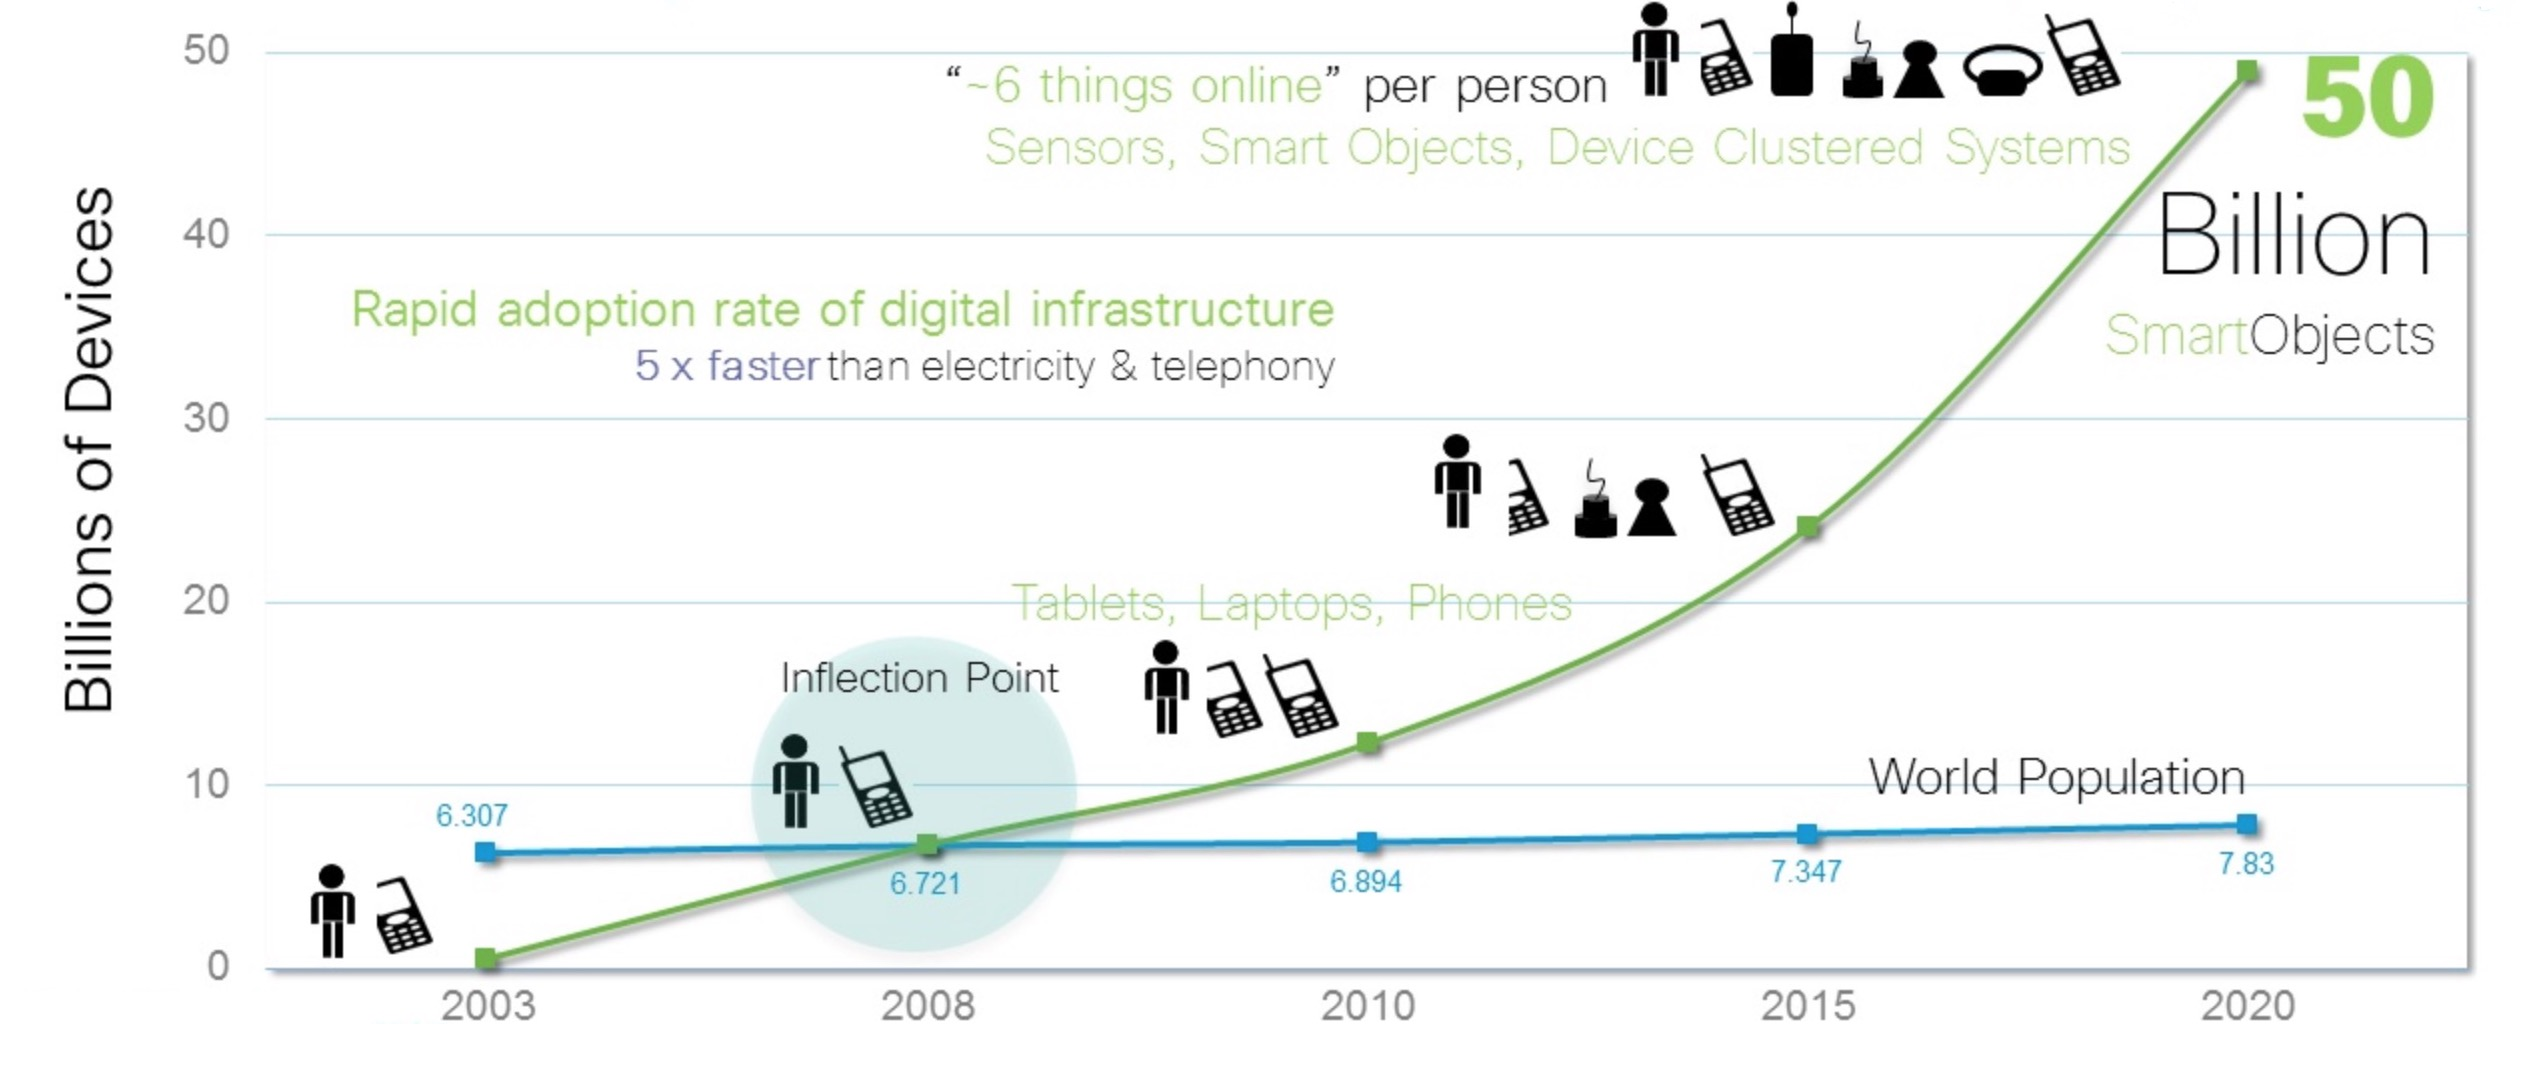
\includegraphics[width=12cm,height=6cm]{/Users/henninghakonsen/Dropbox/Masteroppgave/thesis/latex/images/popTo2300.jpg}
  \caption{\acrshort{iot} Growth \cite{online:IoT2020}}
  \label{pic:IoT2020}
\end{figure}

Currently we are at a point where it all comes down to how these \acrshort{lpwan} perform, which we will have a look at in this thesis. Up until now, \acrshort{iot} devices has communicated directly or indirectly with Internet, but in a rather complicated way. The typical scenario has been that the \acrfull{ue} communicate with a more complex device, often a wireless unit of some kind, and this device communicates with Internet over \acrshort{lte} or a wired connection. While this is an improvement and a step towards a future of connected things - the current mobile technology does not support the expected growth in this area.

The payload sent from \acrshort{iot} devices is usually small, typically 100 bytes or less. However, the load of a \acrshort{lte} device on the current infrastructure, with all the signaling required, is too high. Hence, a simplified technology would allow less signaling and load on the telecoms infrastructure, while also enabling lowered monthly fees as a consequence. Price is always an important factor when choosing a new product. The typical cost of a mobile subscription with \acrshort{lte} and 5-10GB of data per month cost between 30€ and 50€, supporting 50-100 devices. The cost of a subscription over \acrshort{nb-iot} will according to Telenor and Q-Free be around 0.2€. In addition, hardware and installation costs are reduced with \acrshort{nb-iot}. The aim is that an \acrshort{nb-iot} enabled device will cost around 60€. A similar \acrshort{lte} implementation would require a component that does \acrshort{lte} for embedded devices, which costs around 500€. A simple calculation[\ref{equation:ltevslwpa}] of the cost of 300 devices from a parking sensor use case shows that \acrshort{nb-iot} outperforms the current solution. On the left hand side you see \acrshort{lte} specific additions related to installation and montly fees from the \acrshort{lte} embedded device. The montly fees and maintenance comes from the rent of the hardware position. When using the \acrshort{lte} embedded device Q-Free needs to rent a space for it and pay for maintenance and power for that particular place. Note that this is just an outline of one example and certain parameters may change depending on hardware, installation company and network provider.

\begin{table}[H]
\centering
\resizebox{\textwidth}{!}{%
\begin{tabular}{|l|l|l|l|l|l|l|}
\cline{1-2} \cline{4-7}
 &  &  &  & \textbf{NB IoT} & \textbf{LTE} &  \\ \cline{1-2} \cline{4-7}
Sensors per base station (LTE) & 100 &  & \textbf{One time cost} &  &  &  \\ \cline{1-2} \cline{4-7}
Subsciption cost - monthly (LTE) & € 50 &  & Cost of sensor & 60 & 50 &  \\ \cline{1-2} \cline{4-7}
Installation cost - one time (LTE) & € 1 500 &  & Installation cost per sensor & 0 & 5.00 &  \\ \cline{1-2} \cline{4-7}
Montly fees and maintenance (LTE) & € 250 &  &  &  &  &  \\ \cline{1-2} \cline{4-7}
 &  &  &  &  &  &  \\ \cline{1-2} \cline{4-7}
Number of years & 3 &  & \textbf{Montly cost} &  &  &  \\ \cline{1-2} \cline{4-7}
Number of sensors & 300 &  & Subscribtion & 0.2 & 0.50 &  \\ \cline{1-2} \cline{4-7}
 &  &  & Subscribtion 3years & 7.2 & 18.00 &  \\ \cline{1-2} \cline{4-7}
 &  &  & Fees and maintenance & 0.3 & 0.83 &  \\ \cline{1-2} \cline{4-7}
 &  &  & Fees and maintenance 3years & 10.8 & 30.00 &  \\ \cline{1-2} \cline{4-7}
 &  &  &  &  &  &  \\ \cline{1-2} \cline{4-7}
 &  &  & Total cost per sensor & € 78 & € 103 &  \\ \cline{1-2} \cline{4-7}
 &  &  & Total cost 300 sensors & € 23 400 & € 30 900 & +32 \% \\ \cline{1-2} \cline{4-7}
\end{tabular}%
}
\caption{Cost compare of 300 devices. Euro calculated at 9.5 norwegian kroner}
\label{equation:ltevslwpa}
\end{table}

In addition to lower cost and lower complexity there is a demand for increased coverage. Vehicles driving in vast areas, monitoring sensors positioned several meters under ground and devices located in packed cities are dependent of extreme coverage. \acrshort{nb-iot} will add 20 dB to the link margin, giving a huge coverage increase. This will enable such devices to operate while holding the power usage to a minimum.

Another motivator for \acrshort{iot} is the expected easiness of the setup. With todays technology you have to use sensors communicating over bluetooth or Wi-Fi to a common gateway which is connected to the Internet. With a \acrshort{nb-iot} device you will be able to connect directly to Internet, something people without development experience more easily can learn. This will be an additional cause of growth in the number of \acrshort{iot} devices and is yet another reason why we need to properly implement \acrshort{lpwan} to meet the demands.

The idea of some of the new \acrfull{lpwan} is to use the same hardware as \acrshort{lte} and if the customer wants it they will also support software to enable an \acrshort{iot} platform. The most promising technology for sensor networks is \acrfull{nb-iot} and is enabled with a \acrshort{lte} core network as the bearing network. We will discuss how to implement \acrshort{nb-iot} in a \acrshort{lte} network in section, \vref{section:nb-iot-deployment}. This new technology supports an extreme amount of devices as well as them being in a secure environment. Security is a big concern when discussing general network related topics and we will introduce you to some security measurements provided by \acrshort{nb-iot}. Another concern is bandwidth and power consumption as mentioned. The bandwidth is reduced to a minimum and the power consumption is one of the main focuses.

\section{Current status}
\subsection{Internet}
The main idea of the Internet we know today is quite similar to the past, but the scale and reach has outgrown what anyone thought could be achieved. In 2015 Google's data centers achieved high speed transfers up to 1 Petabit. "According to Vahdat, that is enough bandwidth for more than 100.000 servers to exchange data at 10 Gbps each, or transmit all scanned contents of the Library of Congress in under one-tenth of a second"\cite{online:petabitGoogle}. The reason for these data centers is the use of online resources. Offices, as well as home users require more bandwidth and reliability of the services provided from e.g. Google, VPNs, data storage and so forth.
Internet is everywhere and will continue to grow the coming years. As we will discuss in a later section we are seeing signs of a future where literally everything comes online. This includes wearables, industry monitoring and management systems and this will hopefully engage in a smarter and healthier society.

\subsection{Mobile networks}
Norway's GSM network came online in 1993 \cite{online:gsmTelenorNetcom} and Norway has pressured the current technology to reach higher standards from this time. The evolution of wireless radio technology has usually been focused on making it faster, while not prioritizing battery lifetime and simplicity. However, because this technology is used in mobile devices, it is for most users good news. \acrshort{lte} offers high \acrfull{ul} and \acrfull{dl} speeds and good coverage. One problem with \acrshort{lte} and older wireless technologies is that it consumes a lot of power. People are experiencing high speed transfers to their mobile devices, but at a cost draining their batteries. In the future, power efficiency has to be one of the main features of networks established. This is especially the case for sensor networks as these devices need to be connected to a mobile network. Such sensors are often established in remote locations without steady power. Using \acrshort{lte} or some other standard solution would give these devices short lifetime.

\subsection{A closer look at \acrshort{lte}} \label{ssection:lte}
\acrfull{lte} networks consists of some particular nodes for the network to connect to \acrfull{ue} and Internet. We call this structure \acrfull{epc} \cite{online:epc}. In this section we will get a better look at some of the attributes of \acrshort{lte} and the parts which make the \acrshort{epc} network. We really need to understand the underlying network to get a grasp of \acrshort{nb-iot}. Some of the standards we will mention are using proprietary solutions, but most of them are using \acrshort{lte} as the main infrastructure. \acrshort{lte} was introduced in release 8 of the \acrshort{3gpp} in 2008. In a summation by Ericsson they state some facts about \acrshort{lte} from the initial release. \acrshort{lte} from release 8 supported 100Mbps \acrshort{dl} and 50Mbps \acrshort{ul}(Not peak speeds), reduced latency(down to 10ms) and was cost-effective to set up\cite{online:lteIntroduction}. As of release 10 by \acrshort{3gpp}(year 2011) the speeds were at astonishing 1 Gbps \acrshort{dl} and 500Mbps \acrshort{ul}, however the network is not suited for low powered devices.

\subsection{\acrshort{epc}}
\acrshort{lte} is composed by 5 components which interact with each other. \acrshort{mme}, \acrshort{hss}, \acrshort{s-gw} and \acrshort{p-gw} constitutes \acrfull{epc}. See outline of \acrshort{lte} topology in figure, \vref{online:lteTopology}. In this section we will give a short introduction to the key features of each component.

\begin{figure}[H]
  \centering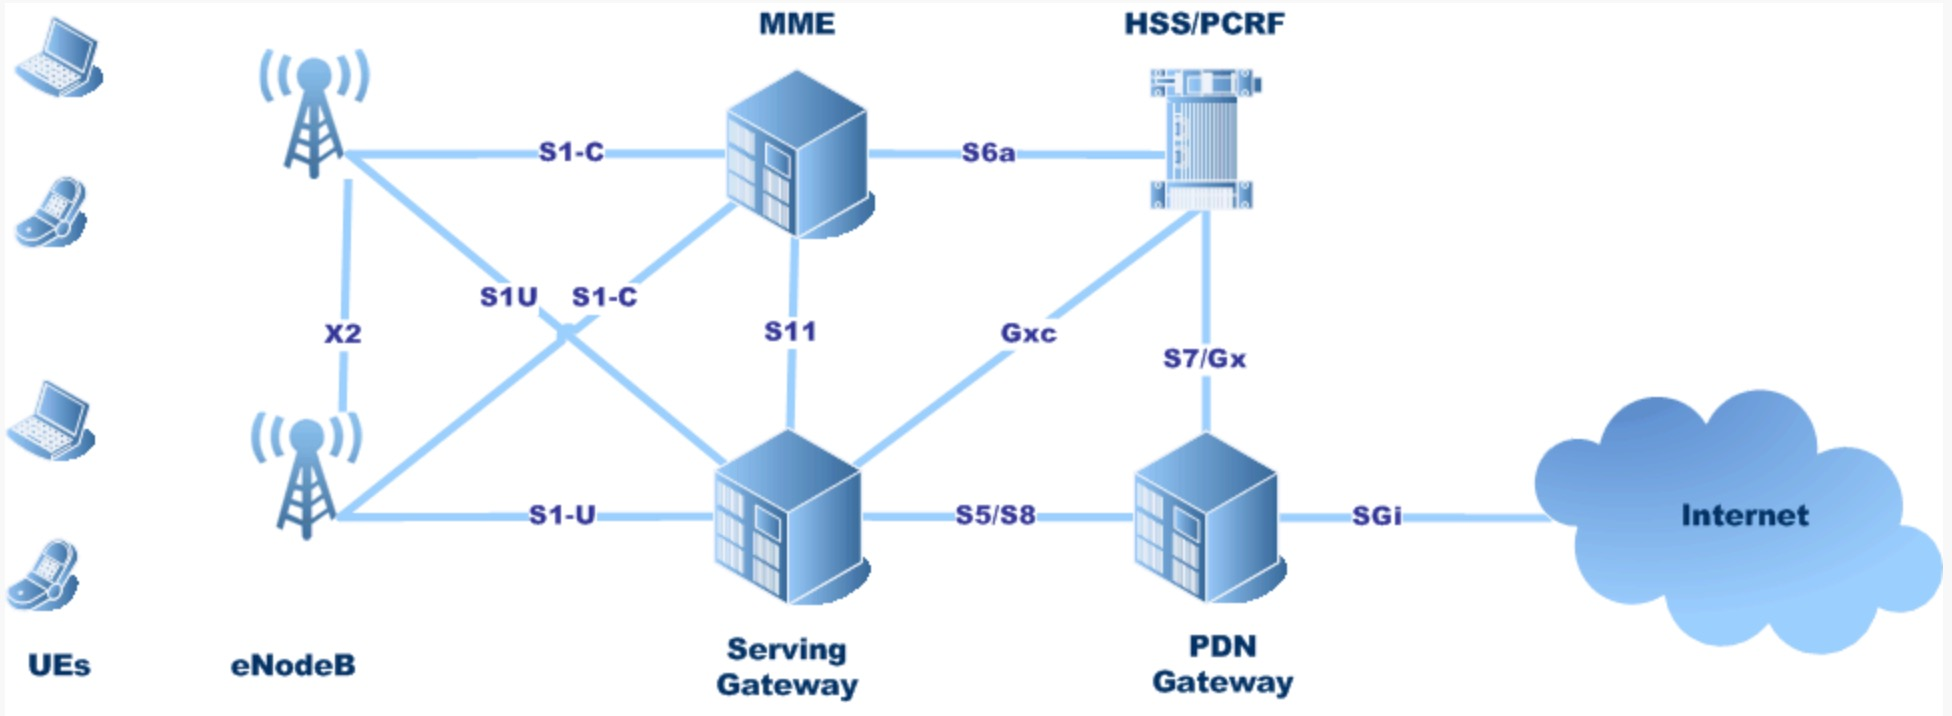
\includegraphics[width=12cm,height=6cm]{/Users/henninghakonsen/Dropbox/Masteroppgave/thesis/latex/images/epc.jpg}
  \caption{\acrlong{epc} \cite{online:lteTopology}}
  \label{online:lteTopology}
\end{figure}
%%http://www.3gpp.org/technologies/keywords-acronyms/100-the-evolved-packet-core
%%http://www.radio-electronics.com/info/cellulartelecomms/lte-long-term-evolution/sae-system-architecture-evolution-network.php

\subsubsection{\acrshort{mme}}
\acrfull{mme} is the main provider of signaling in \acrshort{lte}. \acrshort{mme} is connected to \acrshort{enb}, \acrshort{hss} and \acrshort{s-gw}, through S1-MME, S6 and S11 interfaces. It is in charge of authentication in cooperation with \acrshort{hss} which contains subscriber information, terminal-to-network negotiation and is a part of transition from LTE to 2G/3G.

\subsubsection{\acrshort{hss}}
\acrfull{hss} is the main database for information in the networks. It is a joint service originating from \acrfull{hlr} and \acrfull{auc}. \acrshort{hss} keeps information about subscriber information, that being user identification, addressing and profiles for a subscriber. Profiles describe how the network should perform for this special user and may include parameters like \acrshort{qos}(bandwidth and traffic class) and special modes, or states for a subscriber.
\newline
\acrshort{hss} also holds information about authentication between network and \acrshort{ue}s.

\subsubsection{\acrshort{s-gw} and \acrshort{p-gw}}
\acrfull{s-gw} and \acrfull{p-gw} deal with the user data plane and transports IP packets from \acrshort{epc} to external networks. The \acrshort{s-gw} maintains paths from \acrshort{enb}s to \acrshort{p-gw}s.

The \acrshort{p-gw} is responsible for the communication between the mobile intra network towards the Internet.

\section{Future - mobile networks} \label{section:futureapplications}
For the past ten years we have seen a rise in sensor activity. In the evolution of \acrshort{iot} devices, some has ported to \acrshort{lpwan}. However, as stated in the motivation, \acrshort{iot} devices rely on good coverage and stability. Many people think of home electronics when discussing \acrshort{iot}, but this is not the main goal of \acrshort{lpwan} devices. Oslo's public transport operator(Ruter) has payment cards communicating with activation boxes over RFID, which in turn communicate with Internet. The Norwegian transport agency uses RFID in their tolling stations to communicate with cars. We also see smarter ways to implement these solutions. In the following sections we will give examples of application usage related to future mobile networks. In section, \vref{section:wirelesstech}, we will discuss how to approach technical solutions of future applications.

\subsection{Applications} \label{ssection:applications}
Sensors used for applications are not new. Already back in 2009 a forum called \acrfull{oecd} discussed ways to take advantage of sensors to support a green growth \cite{online:industryApplications}. This forum has members from all over the world, including Norway. The idea is that sensors can surveil and monitor emission numbers as well as act upon them. \acrshort{oecd} came up with a group of applications which were important to investigate. Some of them are smart grids and energy control systems, smart buildings, transport and logistics, agriculture and other general industrial applications. Together these fields combines most of the energy use today and with smarter systems we can reduce power consumption.

With this in mind we can clearly see that many of the fields \acrshort{oecd} discussed has been implemented, or is in the deployment stage. However the current status of industry activities related to these fields are running over 2G/3G/\acrshort{lte} networks. These networks provides average coverage, cost and power consumption, hence with billions of devices enrolling, this is not a sustainable model.

\acrfull{gsma} has made an overview of the most applicable areas of use. In figure, \vref{pic:lpwan}, some bullet points are presented for each area and in the next section we will point out use cases for some of the areas.

\begin{figure}[ht]
  \centering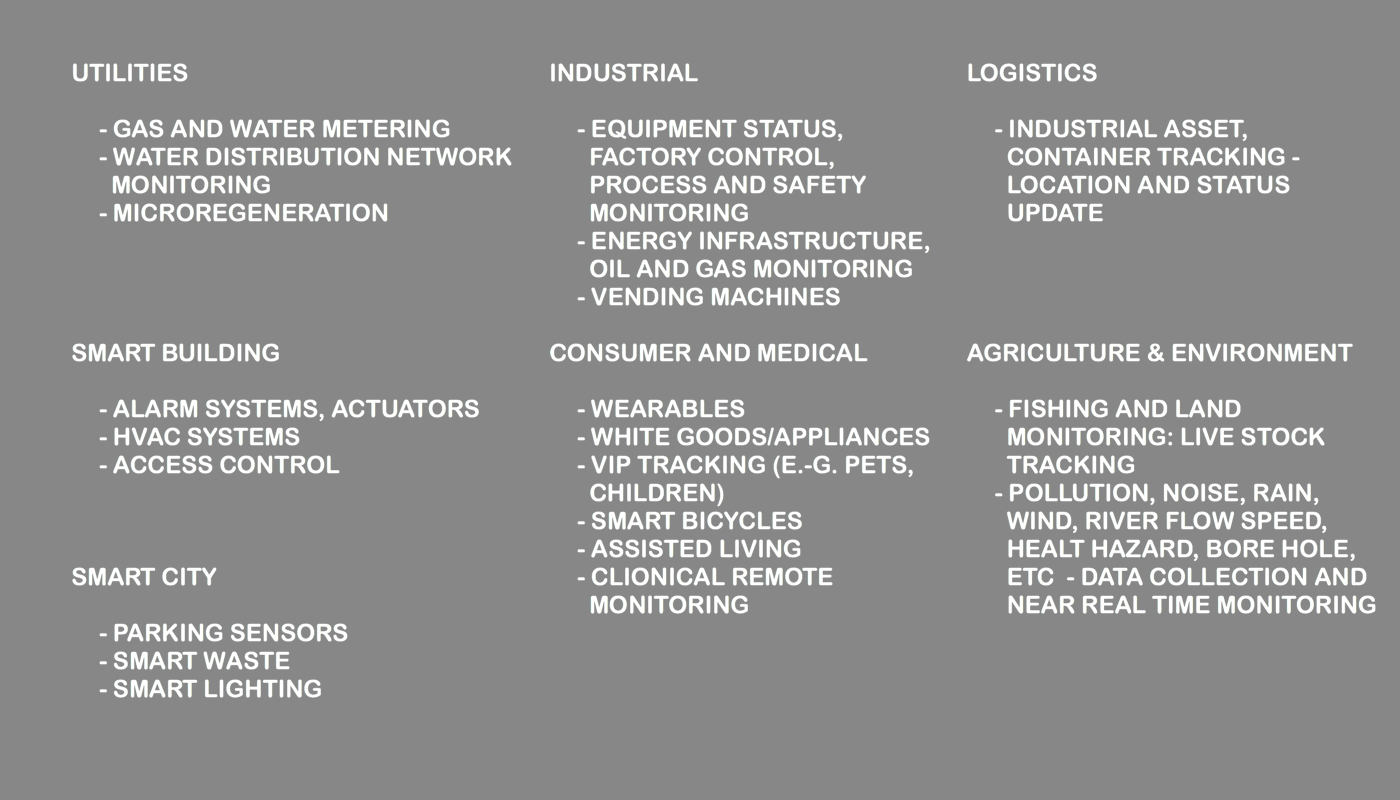
\includegraphics[width=\textwidth,height=8cm]{/Users/henninghakonsen/Dropbox/Masteroppgave/thesis/latex/images/lpwaArea.jpg}
  \caption{\acrshort{lpwan} example applications \cite{online:lpwaFuture}}
  \label{pic:lpwan}
\end{figure}

\subsubsection{Utilities and smart cities}
This domain resolves to what we are investigating in this thesis. Cities are getting smarter by the day and \acrshort{lpwan} can give us the stable network to deploy a large sensor network for monitoring and manage cities. \acrfull{its} is an initiative to control and manage traffic. The system provides communication between cars, trucks and sensors. The sensors are mounted in traffic lights, signs and other objects known in the transport field. The connected devices can adopt to the environment and help the society in several ways. Emergency units can set a route to an accident and the overlaying \acrshort{its} system will clear the way remotely to enable the emergency unit to quickly arrive at the location.

Other usage areas of sensors in cities are e.g. waste areas, power monitoring and \ce{CO2} monitoring. Operations can heavily benefit from more information, as well as automated procedures. There are many use cases where monitoring can be difficult and costly. With simple and cheap devices one could monitor hundreds of different things. As a result the work effort could decrease and the processes can be more efficient. A good example is garbage disposal. If garbage containers were fitted with measuring sensors, the control system can be notified when it is time to empty the garbage. The use case for this will probably be bigger companies and industrial sites, however it might be used for private residents as well.

These devices need to be cost efficient since they will be deployed in large scale. In 2014 a power supplier in Norway called Lyse began installing smart power meters in over 140 000 households \cite{online:lyseAMS}. These devices communicate with the mobile network in the area over a proprietary standard. While it is important to explore new solutions, this is one of many examples where standardized solutions will greatly outperform proprietary solutions.

\paragraph{Parking - a realistic use case} \label{paragraph:sensoroutline}
Big cities are investing in smart parking even though cars may be banned from the cities in some cities. We know that many people will still prioritize traveling with car and facilitating for parking at a nearby location in these cases is crucial. These parking lots can be managed with sensors communicating over \acrshort{lpwan}. For Q-Free next generation parking sensor, they are mainly focusing \acrshort{nb-iot}. The sensor is housed in by a small plastic case which will be leveled with the ground. It withstands extreme forces and detects cars by magnetometer and pulsed Doppler radar. The housing is the most expensive part of the sensor, being able to withstand rough conditions for over 10 years. The idea is that the sensor is drilled into the ground, and will communicate over \acrshort{nb-iot}. The \acrshort{ue} will send status of the occupancy of the parking spot with a fixed interval, as well as reporting parking events when they occur. See \ref{pic:parkingsensor} for a photo of the parking sensor from Q-Free.

As of 2016 the parking sensors communicated to a common gateway(\acrshort{lte} embedded device), a device which communicates with the sensors using a proprietary narrowband communication technology in the ISM band, and to the Internet over \acrshort{lte}. This works fine, but as you might realized, the cost of the devices themselves and managing them are lowered significantly with \acrshort{lpwan} like \acrshort{nb-iot}. Q-Free has chosen to go with \acrshort{nb-iot} since this is the most promising technology providing the necessary requirements for their application. The communication between the sensor and the server is outlined in figure \vref{pic:sensorcommunication}. The sensor sends data to the eNB which in turn sends the data to the \acrshort{iot} platform. If a server has been authenticated within the platform the message is sent to the server. The server receives the packet and can display the message however necessary.

\begin{figure}[H]
  \centering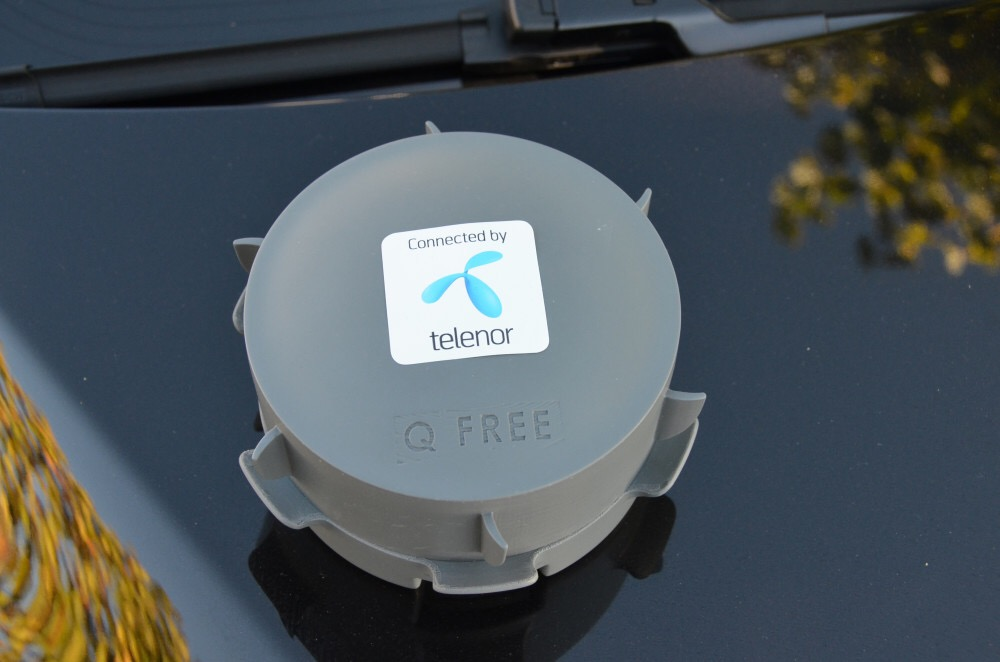
\includegraphics[width=12cm,height=8cm]{/Users/henninghakonsen/Dropbox/Masteroppgave/thesis/latex/images/parkingsensor.jpg}
  \caption{Parking sensor  \cite{person:ola}}
  \label{pic:parkingsensor}
\end{figure}

\begin{figure}[H]
  \centering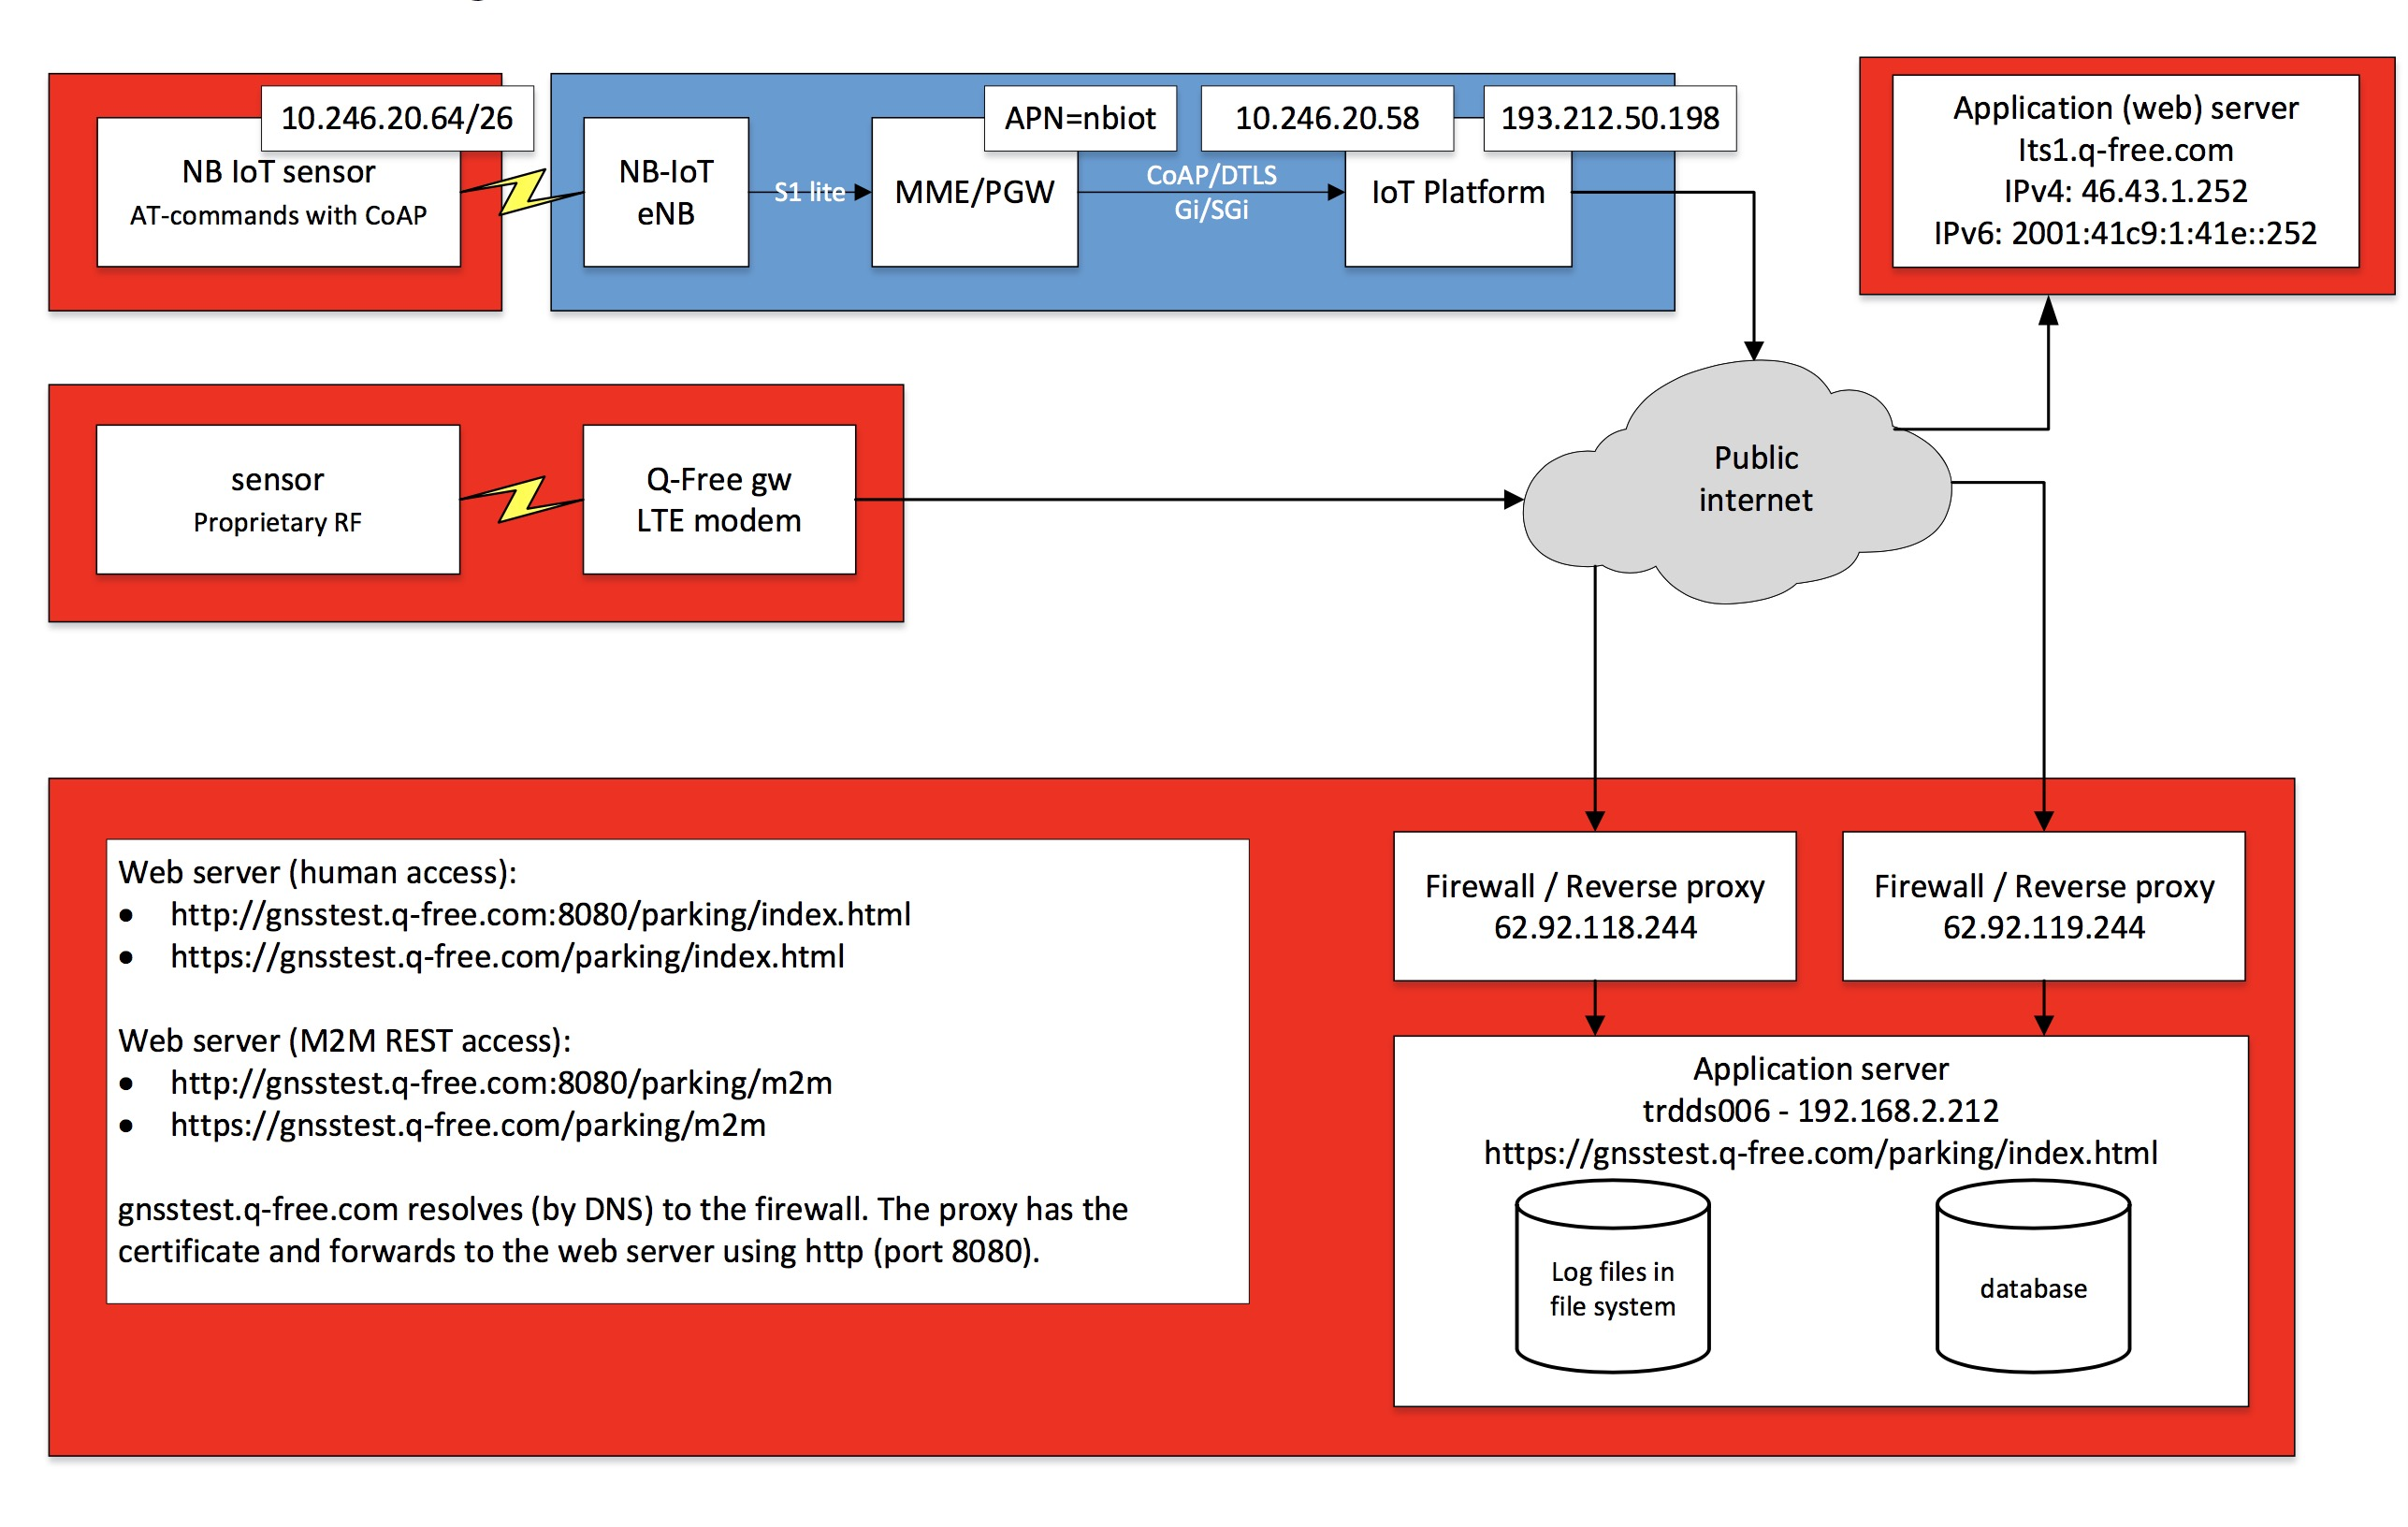
\includegraphics[width=12cm,height=8cm]{/Users/henninghakonsen/Dropbox/Masteroppgave/thesis/latex/images/sensorcommunication.jpg}
  \caption{Outline of sensor communication \cite{person:ola}}
  \label{pic:sensorcommunication}
\end{figure}

\subsubsection{Logistics}
Today parcel tracking is a huge success and some companies are using sensors in their trucks and parcels for real time tracking. Using \acrshort{lpwan} networks will reduce cost of the devices and with long battery lifetime the sensors can be reused. In addition, the coverage for tracing the parcels will have to be great. However, for trucks it might be a better idea to wire the sensor to the trucks power outage. If you want real time, or near real time tracking, the sensor would have to send position data often and this will drain the battery substantially. There are some pros to use \acrshort{lpwan} networks for information collection, but this is probably not the biggest \acrshort{iot} area.

\subsubsection{Industrial}
Industry is a wide area and covers sites like gas stations, construction sites and factories. \acrshort{gsma} also includes vending machines in this category \cite{online:lpwaFuture}. With sensors communicating over \acrshort{lpwan} industry stations can be more automated and it is easier to surveil the systems. Downtime on such systems means lost revenue and efficiency. Low cost sensors which are wireless will hopefully have good coverage and uptime so that these systems run better. This is probably one of the areas where these sensors will be used more frequently since these systems needs realtime monitoring. Another problem solver \acrshort{lpwan} could be for industry use is the excellent coverage. As mentioned good coverage would prevent downtime, but it is also important to notice where some of these sensors will be placed. Factories, sub-sea and underground are some of the locations where industry is often located and therefore coverage is especially important for industry usage.

\subsubsection{Consumer}
Many people think of consumer products when talking about \acrshort{iot}. We are seeing growth in smart watches and smart wearables. The biggest problem with these devices today is the battery life and this is due to the extreme cost of communicating either with your mobile telephone over bluetooth or over \acrshort{lte}. It will be interesting when these watches will use \acrshort{lpwan}. Some wearables, such as your watch may use a standard with higher bandwidth than e.g. \acrshort{nb-iot}. For normal use, one would probably prefer \acrshort{catm} which offers bandwidth up to 1\acrshort{mbit} and could possibly provide music playback and phone calls.

Another interesting use case is smart homes. We have seen a move towards smarter homes for a long time, with better alarms, water and gas metering, light control and so forth. While this usually has communicated over Wi-Fi, there is a potential market where tradition Wi-Fi is not possible or preferable, hence \acrshort{lpwan} can be used.

\subsubsection{Medical}
A potential step into a healthier society is for medical clinics to be able to monitor and give realtime consulting to their patients. The patients device could automatically uploaded real time data to their doctor, enabling them to uncover symptoms or deceases at an early stage and by this increase the average lifetime. One can also collect a lot of data for patients with a special decease and research for a cure. For this to be realistic we really need \acrshort{lpwan} since these sensors will have to be cheap and the stability has to be good.

In Norway we are going into an era where the number of elderly will increase heavily. We should seize the opportunity to use this technology to take care of the elderly. A person which needs attention, but can live alone, would prefer a device which communicates with the care center. The person could also raise an alarm with this system to alert the care takers. In this way the person will probably have a better life and the cost will stay lower.

\section{Developing wireless technologies} \label{section:wirelesstech}
\subsection{The general idea}
As mentioned in the motivation the general idea of new wireless technologies is to reuse the current infrastructure. The new networks will use some combination of \acrshort{lte} and all its components as discussed in section \vref{ssection:lte}. One may also use \acrshort{gsm}, as the current advantage of this network is that the coverage is better at the moment. In a couple of years \acrshort{lte} will be deployed at all locations which GSM covers and we will probably see an increase in coverage as well. Coverage and power consumption are key features of developing wireless technologies and in combination with easiness it is the reason why some technologies stick while others fade away. Easiness is a requirement for \acrshort{lpwan} since the amount of data per packet is relatively small. For some of the technologies, guarantied delivery is not important, but it is important to acknowledge that we may need fast delivery for some applications which uses real time monitoring.
\acrshort{nb-iot} will not suffice for these applications and we need to consider using technologies in parallel or speed up the transmission for e.g. \acrshort{nb-iot}. In the future this may not be a problem considering the pace of wireless evolution, but never the less it is important to not suppress the issue. We know from earlier research that if a user of a platform has to choose between multiple technologies the easiness of the platform impedes.

In the following sub sections we will introduce you to the current comtenders in the competition of concurring the \acrshort{lpwan} market.

\subsection{eMTC/LTE-M and \acrshort{nb-iot}}
\acrfull{emtc} was standardized in the 12th release of \acrshort{3gpp} and updated with \acrshort{nb-iot} in the 13th release. It is meant as an high bandwidth alternative to \acrshort{nb-iot} and is often referred to as \acrshort{lte-m1}.

Both standards are implemented using the current \acrshort{lte} infrastructure, but they differ in coverage, bandwidth and the number of bands used in a cell tower. We see in figure \vref{figure:legacyWire} that \acrshort{lte-m1} provides bandwidth up to 1\acrshort{mbit} while \acrshort{nb-iot} peakes at around 200\acrshort{kbit}(rates from the release they were standardized). The coupling loss of \acrshort{lte-m1} is said to be around seven times better than \acrshort{lte}, and \acrshort{nb-iot} ten times better. We will cover the details about how \acrshort{nb-iot} uses the current infrastructure in section \vref{section:nb-iot}. \acrshort{lte-m1} can be used in the same matter.

\subsection{LoRa \cite{online:LoRa}}
\acrshort{lora} is the most popular non standard solution for enabling \acrshort{iot} devices. It is currently deployed in many cities and uses a proprietary solution. The devices which has a \acrshort{lora} chip uses RF or WiFi to communicate with a common gateway, typically a "cell" tower. The current range is up to 15km, but in dense areas the range only covers 2-5km. The bandwidth is low, but in light of the messages being passed to the gateway that is fine. In figure \vref{figure:LoRa} we see the overlaying infrastructure of a \acrshort{lora} network. It uses many of the same features as we mentioned in the motivation where the devices communicate with a middle box(concentrator/gateway), which in turn communicates with Internet over 3G or ethernet.

\begin{figure}[ht]
  \centering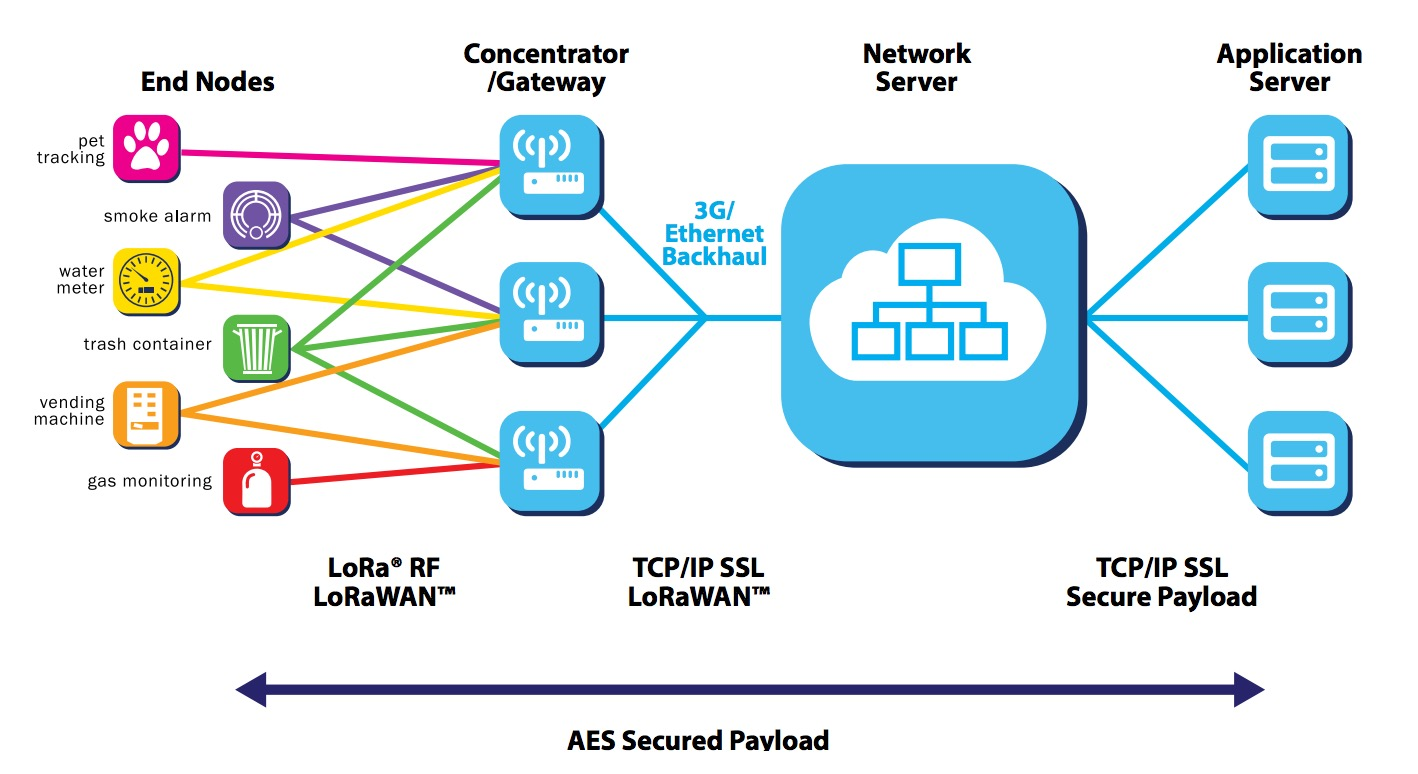
\includegraphics[width=\textwidth,height=8cm]{/Users/henninghakonsen/Dropbox/Masteroppgave/thesis/latex/images/lora.jpg}
  \caption{\acrshort{lora} infrastructure \cite{online:LoRa}}
  \label{figure:LoRa}
\end{figure}

The \acrshort{lora} solution provides an \acrshort{lpwan} at relatively low cost and gives average coverage compared to \acrshort{nb-iot} and \acrshort{lte-m1}. However, \acrshort{lte} is being deployed globally and if the coverage is good enough it will be more costly to provide \acrshort{lora} networks as well as \acrshort{nb-iot} or \acrshort{lte-m1} networks.

\begin{figure}[ht]
  \centering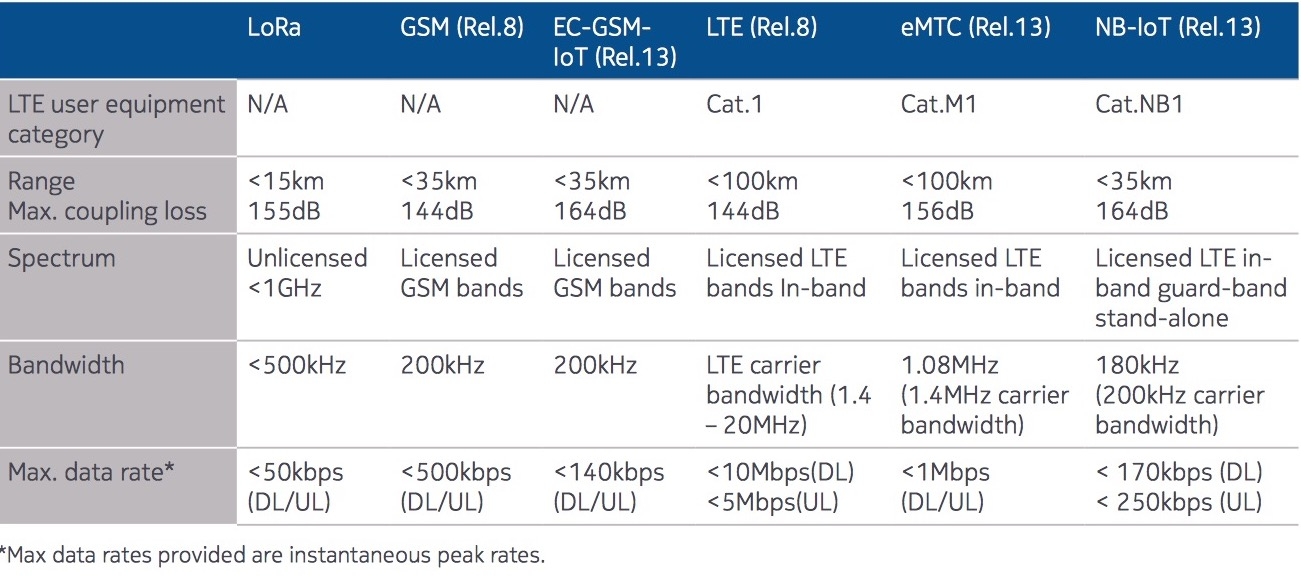
\includegraphics[width=\textwidth,height=8cm]{/Users/henninghakonsen/Dropbox/Masteroppgave/thesis/latex/images/lpwaKeyFeatures.jpg}
  \caption{\acrshort{lpwan} emerging solutions \cite{online:legacyWire}}
  \label{figure:legacyWire}
\end{figure}

\chapter{A dive into NarrowBand IoT} \label{section:nb-iot}
We will focus on a general approach towards \acrshort{nb-iot} as technology and will test both Telenor and Telia's solution. In section, \vref{section:testing}, we will discuss how and where we did the tests as well as giving you examples and results.

Telenor started their \acrshort{nb-iot} network test late 2016, with hardware mainly from Huawei. The goal of the test was to set up a \acrshort{nb-iot} network and test the communication with Q-Free's parking sensors, and run own tests before releasing the network to the public. At the same time Telia had just announced that they had deployed their \acrshort{nb-iot} network, but it was not yet production ready. At the time of delivering this thesis neither Telenor or Telia had \acrshort{nb-iot} in production. Without any specific date they could say that the network would be deployed within a short period of time which indicates that the networks were not in production at the time of our tests, but at a stable state.

\acrfull{nb} \acrfull{iot} is the most promising \acrshort{lpwan} solution and the focusing technology in this thesis. The standard is made by \acrfull{3gpp} and \acrfull{etsi}, and was launched late summer of 2016 with the 13th release of the The Mobile Broadband Standard. The technology takes advantage of the current \acrshort{lte} infrastructure in a very sufficient way. The deployment requires no extra hardware, so the software necessary can be implemented into current hardware. In the following sections we will introduce you to the structure of \acrshort{nb-iot} and the design requirements. We have not emphasized security in this thesis and will only be mentioned in the appropriate sections.

\section{System design}
In a system design process it is important to analyze the use of the new technology. It is crucial to understand how people and the industry will take use of \acrshort{nb-iot}. A good example of a standard which is causing problems today is \acrshort{ipv4}. When this standard was introduced, no one could predict the growth of online devices and for this reason \acrshort{nb-iot} has some specific system design features which hopefully will cover its use for foreseeable years ahead. In the next section we will briefly introduce the system requirements.

\begin{itemize}
  \item Link budget improvement \newline
  The sensors and devices in mind when deploying \acrshort{nb-iot} need better coverage than the average phone or \acrshort{lte} modem. As mentioned these sensors will be used in vast areas, underground and indoors. It is therefor important that the coverage is suited for this use. The goal is to reach 20dB extended coverage compared to \acrshort{lte}. Not only does this extend the range that these devices can be deployed, but they can emit transmissions with lower power, and hence use less power.

  \item Density \newline
  In the article from Cisco \cite{online:IoT2020}, they predict the growth of \acrshort{iot} devices. The prediction is that each household has on average 4 devices. According to Oslo council there are approximately 332 568 households per 1.1.2016 \cite{online:husholdningstatistikk}. This means that if we were to calculate the device pool today it would be around 1.3 million devices only for house holds. Taking into account that these devices will be broadly used by the industry as well, the device density will be very high. To put this into perspective we can investigate the device density of \acrshort{gsm}. For each \acrshort{gsm} cannel (200 KHz) there are 8 time slots, giving 8 concurrently connected devices. In one cell tower there are approximately 8 channels, and they are often split between mobile providers. If we assume that all of them belong to one provider, one cell tower can support up to 64 devices concurrently. One \acrshort{gsm} cell tower will provide coverage for the surrounding 1km, and since cell towers to close to each other will cause interference only one cell tower can provide coverage for 1km in radius. \acrshort{lte} has much more resources and can provide coverage for more devices, using time and wave division multiplexing.

  There is however a presumption to why \acrshort{nb-iot} can support so many devices per carrier. In the specifications one \acrshort{nb-iot} channel can support more than 50 thousand devices and keep in mind that \acrshort{nb-iot} can be deployed in one \acrshort{gsm} channel, which only supported 8 devices. The way this is supposed to work is due to the infrequent updates from the devices. One device might send a message every second hour and another might even send messages only once every day. One scenario where this might cause problems is if every programmer/company sends updates on specific times. Typically one would want updates at the hour marker(ie. 14:00, or 15:00). If thousands of devices do this at the same time, congestion and latency will definitively effect the experience for the devices.

  \item Low complexity \newline %%low cost
  A key feature for the devices supporting \acrshort{nb-iot} is that the complexity level is low. The new standard is less intricate than ordinary \acrshort{lte} which means that the devices can be less complex, resulting in cheaper hardware. This is an important factor for success since these devices need to be cheap to be broadly deployed. The complexity in this technology resides in the core mobile network for it to support many devices. Other than this, the technology supports average speed and average latency, perfect for monitoring purposes.

  \item Low power \newline
  The power consumption of the communication needed for \acrshort{lpwan} need to be low for the estimated battery lifetime of a device to be kept. The goal is over 10 years of lifetime, and since these devices probably will be very cheap, it might be cheaper to change the device instead of changing the battery.

  Low complexity and better coverage will help the device to consume less power, but it will not enable the device to operate for 10 years. The system design includes a special operation mode, called \acrlong{psm}. We will elaborate how this key feature will work in section \vref{ssection:psm}.

  \item Latency \newline
  For most applications applied to this new technology, latency is not key feature. We would like the device to send frequent, or infrequent message to a server or another device, but the time used is not important. However, what is actually a long time? A ping request on a normal wired connection today uses around 5-100ms, and even less for fiber connections. On mobile networks like \acrshort{lte}, the usual ping time is on average higher than on a wired connection, but usually it does not exceed 100ms. \acrshort{nb-iot} aims at a peak latency of 10 seconds. In comparison that is 100 times longer than a normal \acrshort{wan} connection, but it should suffice for most applications using \acrshort{lpwan}. The latency could probably be lowered, but it might interfere other design features, such as device density.

  \item Security \newline
  A big issue in Internet today is security, specially \acrshort{ddos} attacks. These attacks are more frequent and is an attack form which enables thousands of machines to continually spam one or several IP addresses, which in practice disables the application. In the fall of 2016, the DNS service provider "Dyn" was down because of a \acrshort{ddos} attack. Being a big DNS server, Dyn's downtime impacted major Internet platforms in both USA and Europe \cite{online:ddosAttack}. Since an attack like this needs a huge device pool it is likely to think that \acrshort{iot} devices are a potential tool for hackers. If hackers could access millions of devices with Internet access, they could easily perform global \acrshort{ddos} attacks which would halt our infrastructure, in turn disabling many of us to do our jobs.

  With this in mind, the engineers and designers of \acrshort{nb-iot} needed to consider security issues like this. We mentioned the \acrshort{iot} platform when discussing the deployment in section \ref{section:nb-iot-deployment}. This platform is the glue of \acrshort{nb-iot} and also a huge contributor of security measures in cooperation with \acrshort{mme} and \acrshort{hss}. The system requirement of \acrshort{nb-iot} is that no one should be able to directly access a \acrshort{nb-iot} device. One additional security feature in general with mobile networks is SIM cards. Like cell phones, \acrshort{nb-iot} devices will be fitted with a SIM card, which will enable the core network to authenticate the device, and visa versa. The SIM card has a subscription connected to the service provider, hence making a strong authentication scheme.
\end{itemize}

\section{Deployment} \label{section:nb-iot-deployment} %% Done, but might be nice to add HH legge til info om deployment i et LTE nett
In figure \vref{online:lteTopology} we saw the current infrastructure of \acrshort{lte}. To manage security issues and new features, a solution is to introduce a new term called \acrfull{iot-platform}. This platform will keep track of communication between outside applications and inside nodes. In theory the communication would suffice without this platform, but due to the extreme security issues regarding sensors we need a way to authenticate traffic. Many \acrshort{iot} devices are easy to hack and can be used for \acrfull{ddos} attacks. We have seen many service struggling with downtime due to overloading of their servers because of \acrshort{ddos} attacks. The platform ensures that traffic between two entities is secure, where one being the sensor and the other being the application server. For an application to receive traffic from a sensor, it will have to negotiate with the \acrshort{iot-platform} to gain access. After the setup procedure the \acrshort{iot-platform} acts as a \acrshort{nat} device, as well as matching correct application to correct user group, often called subscription. We might see other solutions for securing the internal network without negotiations.

\acrshort{iot-platform} is just one way to solve these issues. This software is in fact just an application proxy, or a firewall. Either way it can be implemented in the current hardware, but it is also possible to provide an extra rack mounted device to deal with this. In Telenor's test case, spring 2017, all the servers/hardware required was located at one location and the \acrshort{iot-platform} was running on private hardware from Huawei.

\subsection{Operation modes} \label{ssection:operationmodes}
\acrshort{nb-iot} occupies 180kHz bandwidth and there are currently three ways to integrate \acrshort{nb-iot} with \acrshort{lte}. The available operation modes are standalone, in-band and guard-band - see figure \vref{figure:nbiot-operationmodes} for illustrative definition. Standalone operation uses a dedicated GSM/\acrshort{lte} channel, utilizing the ability to deploy \acrshort{nb-iot} in \acrshort{gsm} as well as \acrshort{lte}. In figure \vref{figure:nbiot-operationmodes} we illustrate this operation mode to point out that \acrshort{nb-iot} can be deloyed in \acrshort{gsm}, even though this is not for the long run.

In-band operation utilizes bandwidth within one \acrshort{lte} carrier. This is the most technical and advanced solution and requires more work by the network provider. The reason for this is because of interference between the \acrshort{lte} and \acrshort{nb-iot} sections in the carrier. When deploying in-band \acrshort{nb-iot} allocates three resource blocks of an \acrshort{lte} channel.

Guard-band operation makes use of the bands not in use by \acrshort{lte} due to interference between \acrshort{lte} carriers. This in-between section is called a guard band and guards the carries for interfering with each other. This band can be used by \acrshort{nb-iot} and is a solution where one would want to utilize all resources of a cell tower.

\begin{figure}[ht]
  \centering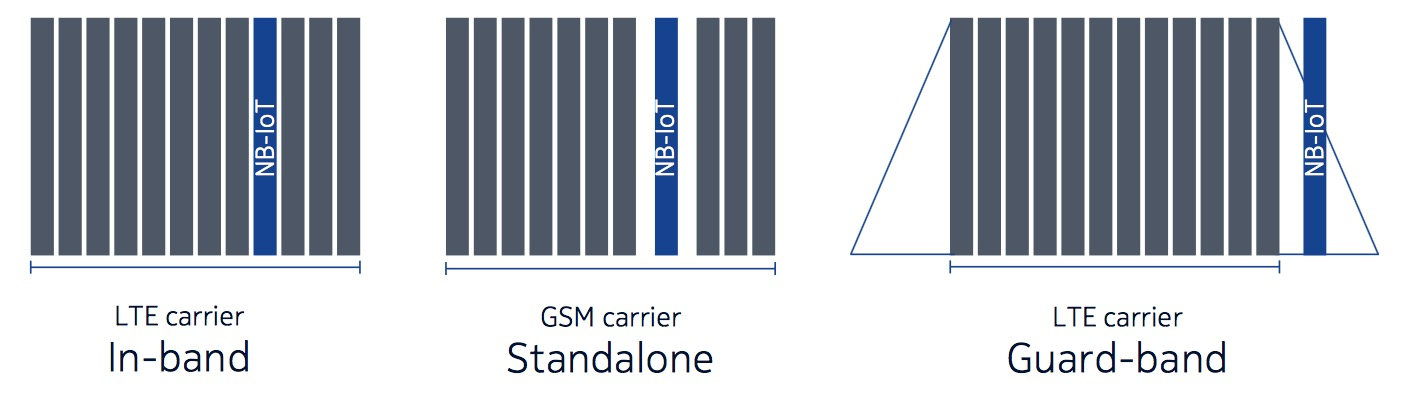
\includegraphics[width=12cm,height=4cm]{/Users/henninghakonsen/Dropbox/Masteroppgave/thesis/latex/images/nbiot-operationmodes.jpg}
  \caption{\acrshort{nb-iot} operation modes \cite{online:legacyWire}}
  \label{figure:nbiot-operationmodes}
\end{figure}

\section{Introduction to energy saving} \label{section:energysaving}
Power saving is an important part of mobile communications for sensors. Several techniques are used to reduce power consumption, and \acrfull{drx} and \acrfull{psm} are two of them. \acrshort{drx} has existed for 20 years and is implemented in \acrshort{lte}, while \acrshort{psm} was introduced with the development of \acrshort{lpwan}. These two modes, together with paging\ref{ssection:paging} introduces an improved network, especially suited for sensors. In figure \vref{figure:nb-iot-timeconverge} you can see an outline of the communication process for a device. RRC Connected mode is the mode where the device actually can communicate with the network. The following procedures shows a possible time convergence graph for a device. We will explain the techniques used, as well as the specific time periods of the figure in the next sections.

\begin{figure}[ht]
  \centering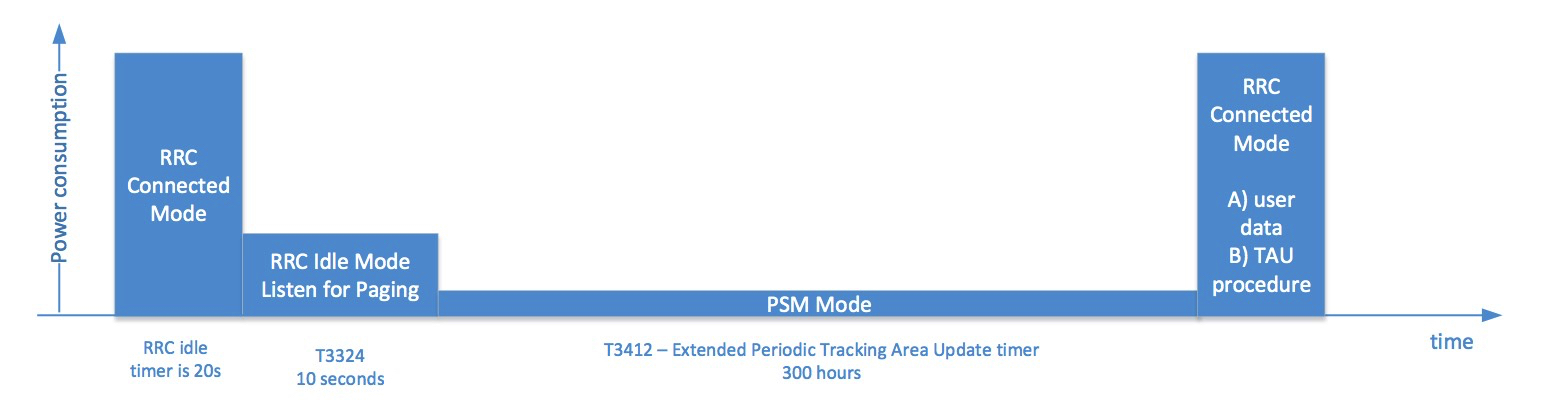
\includegraphics[width=12cm,height=6cm]{/Users/henninghakonsen/Dropbox/Masteroppgave/thesis/latex/images/nb-iot-timeconverge.jpg}
  \caption{\acrshort{nb-iot} time convergence \cite{person:ola}}
  \label{figure:nb-iot-timeconverge}
\end{figure}

\subparagraph{Prerequisites}
To get a good understanding of the results we need to closely look at the outcome of the results and understand the meaning. In the following sections will describe details about how \acrshort{nb-iot} works and what the specifications are saying. As stated we will be mostly focus our tests on coverage and power usage, which relates closely. Coverage is measured in \acrfull{dbm} and provides a relation between the distance between the base station and the \acrshort{ue}, and the transmit power of the \acrshort{ue}. In theory a device will transmit with the relative strength according to the coverage, so that the signal is received at the base station. Depending on the coverage of the device it will adjust the transmit power.

With this in mind we can convert coverage and transmit levels to output power. In worst case scenarios the device will transmit data with ${+23\acrshort{dbm}}$, which under normal circumstances is converted to ${230 \acrshort{ma}}$ \cite{datasheet:ubloxchip}. We can convert \acrshort{dbm} to \acrshort{mw} by calculating ${10^{x \acrshort{dbm} / 10}}$. Keeping ${+23 \acrshort{dbm}}$ in mind gives us ${10^{23 / 10} = ~200 \acrfull{mw}}$. We can also convert from \acrshort{ma} to \acrshort{mwh} by multiplying \acrshort{ma} with the voltage of the chip at 3.3 volts, gives us ${230\acrfull{ma} * 3.3V = 759 \acrshort{mwh}}$.

\acrshort{nb-iot} operates between ${-40 \acrshort{dbm}}$ and ${+23 \acrshort{dbm}}$, where ${-40 \acrshort{dbm}}$ equals ${10^{-4} = 0.0001 \acrshort{mw}}$ and ${+23 \acrshort{dbm}}$ equals ${10^{2.3} = 200 \acrshort{mw}}$. We will see how this will influence the power usage in the tests and we will also touch on the subject in the following section.

\subsection{RRC connected mode} \label{ssection:rrc}
This mode is used when the device wants to communicate with the network, either \acrshort{ul} or \acrshort{dl}. The time spent in RRC connected mode can vary, but the default \acrshort{nb-iot} timer is 20 seconds. In this mode the device will use a lot more power, hence we want to move away from this mode as soon as we are finished transmitting or receiving data. When the chip is in active/connected mode it uses ${6 \acrshort{ma} = 0.006 \acrshort{a} * 3.3V = 0.0000198 \acrshort{mwh}}$.

When the transmit operation is finished the chip will stay in connected mode until the time period ends. There is an optional flag, "release assistance indicator", in the AT send command which puts the device into \acrshort{psm} directly after the transmit operation. The network needs to support this action to give the \acrshort{ue} permission to sleep. It is the network which decides what the \acrshort{ue} should do according to the network and the devices status. Given that the network supports release assistance indicator the battery life would be extended, since we only send data for a short period rather than waiting for downlink data which in many applications is not needed.

The calculated numbers in this section are based on specifications from the manual of the \acrshort{nb-iot} chip\cite{datasheet:ubloxchip}. We will try to test and verify these numbers in section, \vref{section:detailedtest}.

\subsection{RRC idle mode}
After ending RRC connected mode the device enters RRC idle mode listening for paging, using approximately 1mA. The default \acrshort{nb-iot} time is 10 seconds and in this mode the device can receive data from the network with a paging request, meaning that there is data for the device in the network. If there is more data in the network the device will re enter RRC connected mode and try to receive data from the network. If there is no more data for the device it can enter \acrshort{psm} or \acrshort{edrx}

\subsection{\acrfull{edrx}} \label{ssection:edrx}
\acrfull{drx} is a way in \acrshort{lte} to keep the device connected, but reducing the power usage by only checking for new data(paging) on time slots. After a sequence of communication the device goes into a \acrshort{drx} state where it periodically checks if the network has new information for the device. If there is information for the device, the device enters RRC connected mode where it can receive and send data. In the figure the \acrshort{drx} time(\acrfull{T3324}) is set to 10 seconds, after a period of 20 seconds in RRC idle mode.

When designing \acrshort{nb-iot}, \acrshort{drx} had to be implemented. However if the device always checks for paging the battery would decrease at a high rate. \acrshort{edrx} is therefor an outcome of the idea of \acrshort{drx} in the special case of sensor networks. It is a new way to handle communication for sensors which needs to wake up for certain events or messages from the network. In an article about \acrshort{edrx} and \acrshort{psm} for \acrshort{lte-m1} we find a great figure showing \acrshort{edrx} \vref{figure:edrx}. Even though this is for \acrshort{lte-m1} it applies for \acrshort{nb-iot} as well. After a device has communicated, either sending or receiving packets over the network, we want it to use as little power as possible. By default the device will enter \acrshort{drx} mode for a network-specified time and if configured go into \acrshort{psm} mode after the given time. As mentioned, for some applications we want the device to be able to receive packets without waking it self up.

The device will then go into \acrshort{edrx} instead of \acrshort{psm} mode. This means that for the most of the time the device will sleep, but periodically it will check for new information(paging). The period where the device sleeps is configurable in the network. Since the internal clocks in the devices often are unreliable, and the time between these syncs may be long(typically 1-2 hours), we need to first sync the clock and information between the device and the network. We call this operation sync guard. We have to do this due to communication based on time(time slots/\acrlong{tdma}). After this process the device will operate in normal \acrshort{drx} mode for a certain period(~10 seconds) and go to sleep after that period. This is a very power efficient way to keep the device more synchronized with the network, but it raises some practical problems. (either remove the last sentence or discuss it later). In the parking use case we only need to send information, hence we don't need to activate \acrshort{edrx} mode.

\begin{figure}[ht]
  \centering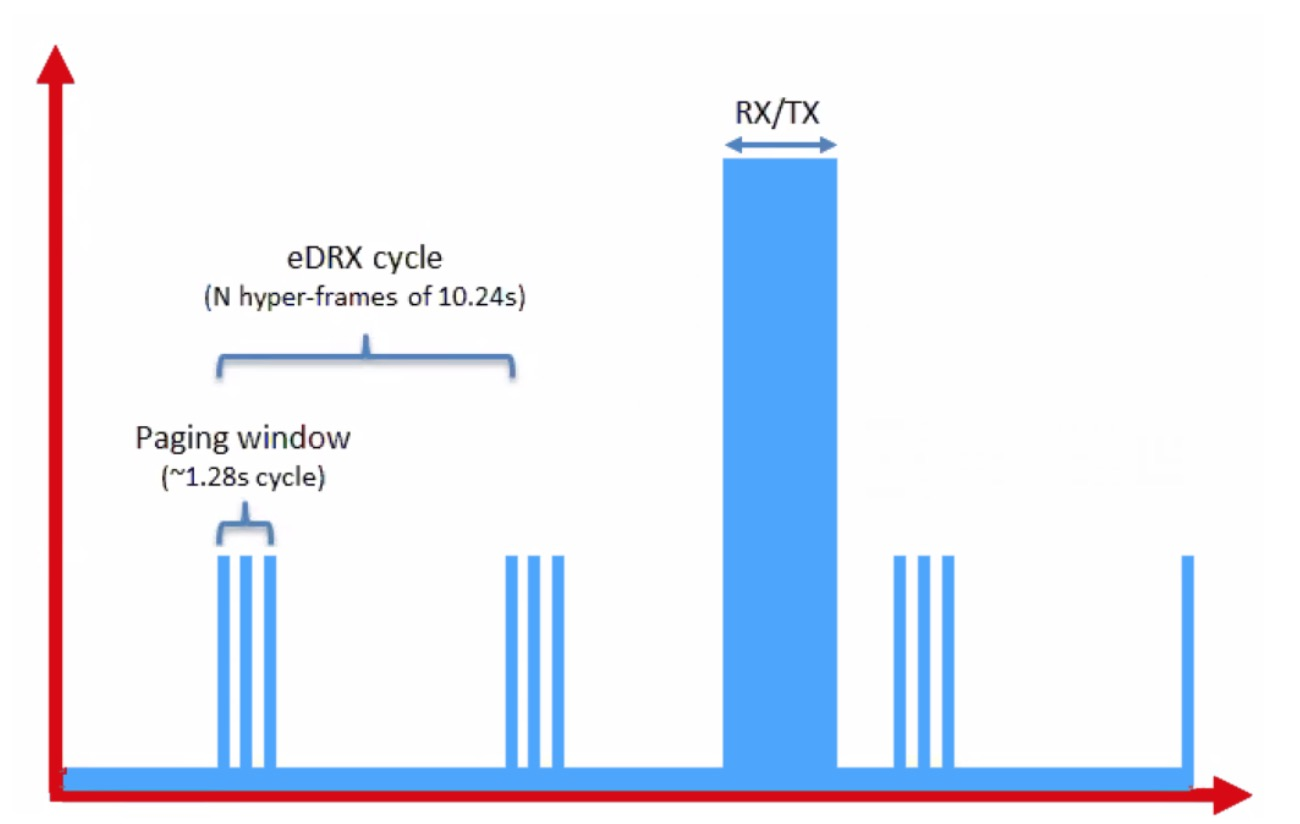
\includegraphics[width=12cm,height=6cm]{/Users/henninghakonsen/Dropbox/Masteroppgave/thesis/latex/images/edrx.jpg}
  \caption{\acrshort{edrx} operation mode \cite{online:edrxpsm}}
  \label{figure:edrx}
\end{figure}

\acrshort{edrx} has a set of configurable parameters which define how the \acrshort{ue} behave when entering \acrshort{edrx} mode. In short terms we want to specify \acrshort{edrx} cycle length and paging time window. The cycle length is the length of an \acrshort{edrx} cycle. This means the time from start of a period to the start of the next period. The cycle length can vary from 5 to 2621 seconds. The paging time window can be set to 0 to 20 seconds, where the value 0 means that paging is not in use. In section, \vref{ssection:paging}, we describe what paging is.

\subsection{\acrfull{psm}} \label{ssection:psm}
\acrshort{psm} is the core of power saving in \acrshort{nb-iot}, as well as many other \acrshort{lpwan}. The idea of almost all \acrshort{lpwan} is that the devices send information periodically, while sleeping 99\% the rest of the time. After a typical connected period we want to enter a sleeping mode where very little power is drawn, usually by an internal clock. This mode is called \acrshort{psm} and enables the device to sleep for a network configured time period. In our test case this time(\acrfull{T3412}) is set to 300 hours, almost two weeks. That means that the device will be removed from all meta data in the \acrshort{mme} after 300 hours if there is no communication. This technique is foremost for the devices which only sends information to a server. The way it works is that the device goes from connected mode, to \acrshort{drx} mode listening for information from the network. After this the device enters \acrshort{psm} mode if activated. When in \acrshort{psm} mode the only thing going on in the device is an internal clock which can start the system at a specific time. This is necessary since we want the device to wake up at a specific time and perform POST/SEND operations towards a server.

In \acrshort{psm} the chips power usage will be as low as 3$\mu$A, which is extremely low and the main reason why we can expect these types of sensors to achieve 10 years of battery lifetime.

%%http://www.link-labs.com/blog/lte-e-drx-psm-explained-for-lte-m1
\subsection{Paging} \label{ssection:paging}
Paging is a procedure to initiate communication from the network. If paging is enabled the \acrshort{ue} will listen for data from the network at given time intervals within a RRC idle or \acrshort{edrx} period. If the serve wants to communicate with the sensor it sends a message over the network and it will be stored at the IoT Platform until the device is paged in.

\subsection{ECL} \label{ssection:ecl}
As mentioned in section, \vref{ssection:rrc}, the \acrshort{ue}s will enter different coverage modes based on their signal strength towards the base station. There are three levels of \acrfull{ecl}. At which coverage level devices switch over to the different levels is decided by the network. Telia uses ${-105 \acrshort{dbm}}$ for \acrshort{ecl}1 and ${-115 \acrshort{dbm}}$ for \acrshort{ecl}2 \cite{mail:teliaMailThread}, coverage better than this resolves to \acrshort{ecl}0. OML Telenor?

\acrshort{ecl} is not important by itself, but an application fetching the \acrshort{ecl} of the device will gain a lot of information about the reception, hence it might reconfigure the setup of the transmit process for example. Because, based on the signal strength the device will retransmit data to improve \acrfull{tsr} towards the application server. In \acrshort{ecl}0 the device will transmit the data once, and in level 1 and 2 the \acrshort{ue} will retransmit the data to ensure delivery of the packet. In section, \vref{ssection:ecltest}, we will give you insight in the transmit process of two transmits, one with \acrshort{ecl}0 and one with \acrshort{ecl}2. The difference is big and will definitely affect the battery lifetime of the device.

\subsection{The transmit procedure} \label{ssection:transmitprocedure}
We have looked at several techniques for \acrshort{nb-iot} and the specifications looks very good when the \acrshort{ue} has good coverage. In good coverage areas devices will transmit data with ${-40 \acrshort{dbm}}$, with an average actual transmit time of ~200ms. However in worst case situations, the sensor will boost the signal up to ${+23 \acrshort{dbm}}$, which in terms of power usage is two million times as high, ${(10^{2,3}) / (10^{-4}) = ~2 000 000}$. In addition, as stated, a sensor with bad reception will try to retransmit data. Depending on the coverage the device will enter different coverage modes, described in section \vref{ssection:ecl}. Given that the sensor has bad coverage, and is operating in \acrshort{ecl}2 mode the transmit time might be as long as 5 seconds for a single data transmit. The actual power usage increases rapidly and the chip would use 200\acrshort{mwh} for 5 seconds, resulting in a power usage of ${((200 \acrshort{mwh} / 60 / 60) * 5S = 0.27 \acrshort{mwh}}$, which actually is 50 million times increase in power usage compared to optimal conditions. However, as we will see in our tests, ${-40 \acrshort{dbm}}$ is normally not possible to achieve.

In the following figure, \vref{figure:ecl_dbm}, we see an outline of how the device chooses \acrshort{ecl} mode dependent on the signal quality. In theory the device should lower its transmit power equally to the signal strength. The graph represent the theory behind the adjustment of the transmit power and you will see how this actually works in section, \vref{section:testing}.

%%https://cdn.rohde-schwarz.com/pws/dl_downloads/dl_application/application_notes/1ma266/1MA266_0e_NB_IoT.pdf

\begin{figure}[H]
  \centering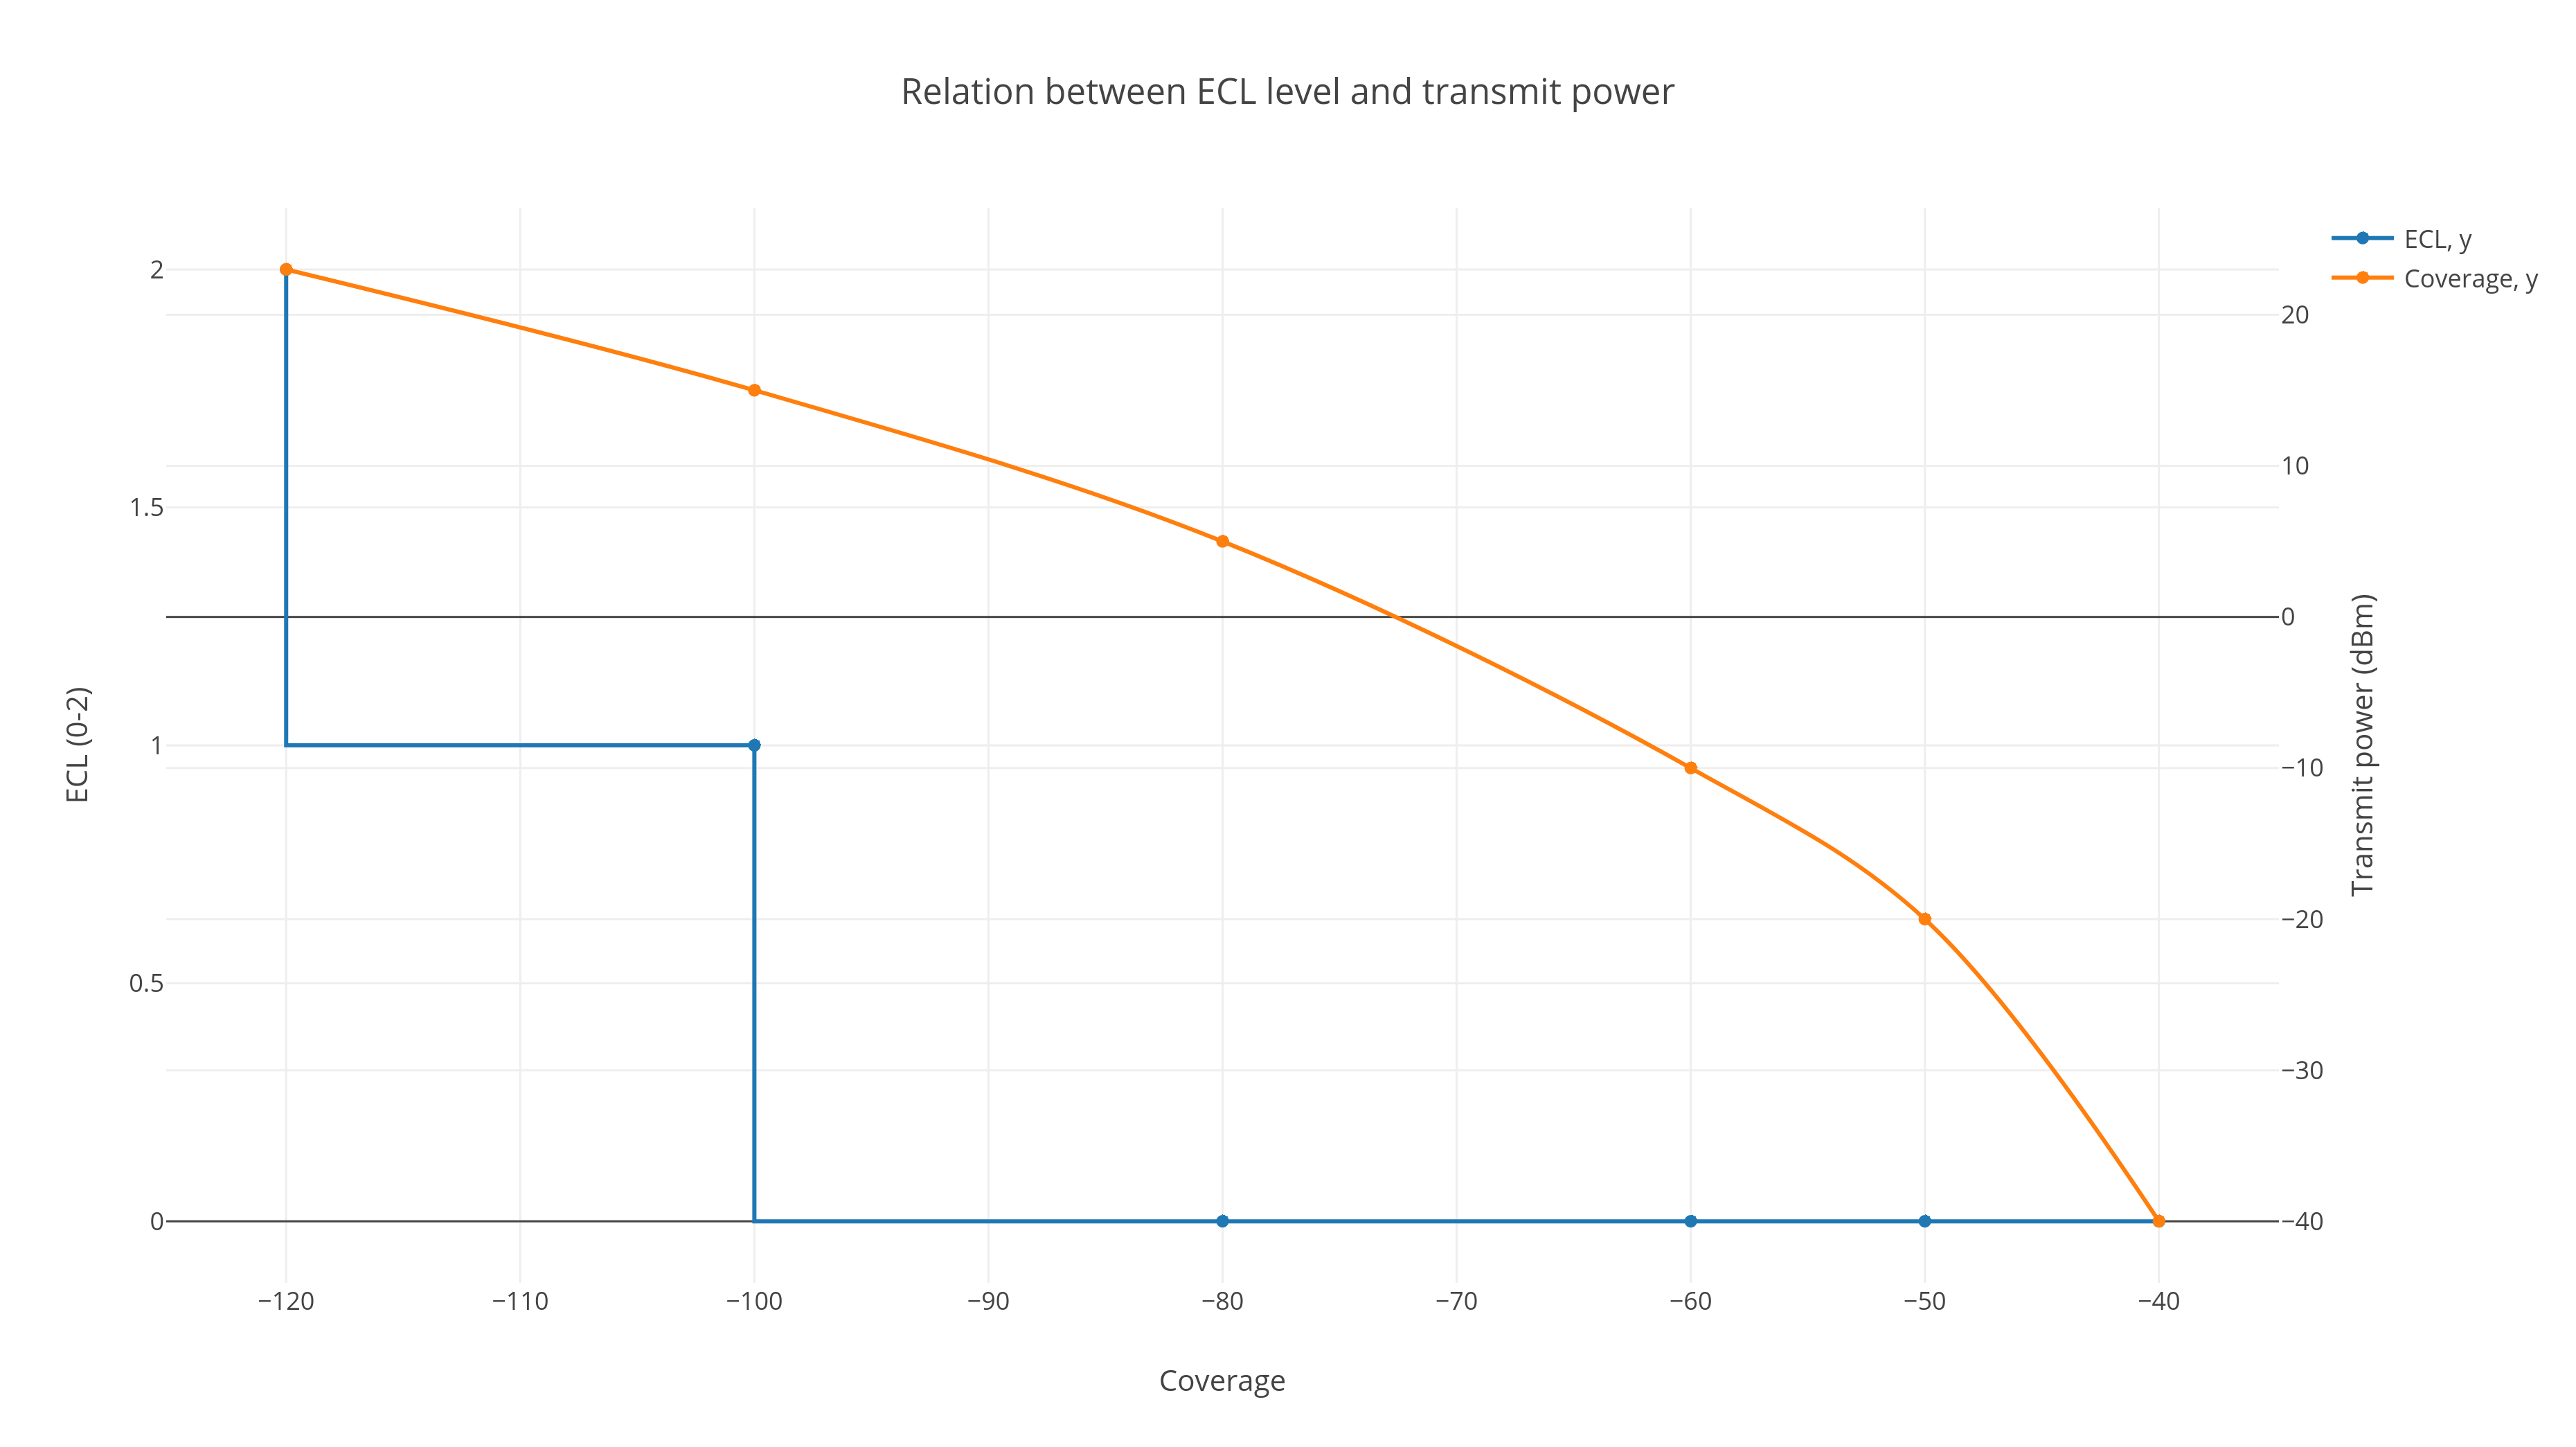
\includegraphics[width=\textwidth,height=9cm]{/Users/henninghakonsen/Dropbox/Masteroppgave/thesis/latex/images/ecl_tx_power_relation.png}
  \caption{\acrshort{ecl} and \acrshort{dbm}}
  \label{figure:ecl_dbm}
\end{figure}

\section{The current market and deployment strategies} \label{section:market}
We have discussed several applications which suit \acrshort{lpwan} and there is a demand for chips which implement \acrshort{nb-iot} or \acrshort{lte-m1}. In this section we will give you a brief introduction to the key firms involved with \acrshort{lpwan} and how the market looks like early 2018.

\subsection{Manufacturers and stakeholders} \label{ssection:manufacture}
There are many companies which manufacture hardware for the mobile industry. Historically Neul(UK), HiSilicon(China) and Qualcom(USA) has been the main chipset producers. Neul and HiSilicon is owned by Huawei which makes them one of the biggest producers at the moment. In addition there are three companies, Ublox, Telit and Quecktel, which have been using "Huawei" chipsets, only adding their custom software. At the moment the agreement towards Huawei has expired and the three software companies will need to fetch hardware from another manufacturer, which will most likely be Qualcom.

Currently there is a problem surfacing in USA which stresses the market. In Europe GSM/GPRS has been the only alternative, while in USA there has been three network technologies, GSM/GPRS, IS95 and TDMA. Because of the different technologies the process of developing chipsets has been difficult and they have now decided to take down IS95 and TDMA. Most users have gone over to LTE, but there are many companies which use IS95 and TDMA for low powered devices which now has no good alternative. The solution is to move over to another \acrshort{lpwan}, which for most companies will resolve to \acrshort{lte-m1} because of the opportunities and spread of applications this technology provides.
Because of the stress in the market and the increased demand for general \acrshort{lpwan}, all chipset manufacturers began their work on \acrshort{nb-iot} and \acrshort{lte-m1} chipsets. Most of the companies did however reuse their \acrshort{lte} chips to produce a \acrshort{lpwan} chipsets. The chip we will be using is produced by Neul, with software from Ublox, and suffers from the process of reusing hardware originally developed for \acrshort{lte}. In section, \vref{section:thechip}, we will give you a detailed introduction to how we used the chip, but it is worth noting that the chip was not production ready.

Other companies have seen the development of this market and started to take up the fight against the biggest companies. Nordic Semiconductor is one of these companies, and originally has produced chips for other technologies like bluetooth. According to a talk they gave, they have used 1.000.000 working hours on chips with \acrshort{lte-m1} and \acrshort{nb-iot}, which is developed from scratch focusing on \acrshort{lpwan} technology. They have seen the stressed market in USA and will begin production of \acrshort{lte-m1} chips this year, followed by \acrshort{nb-iot} in 2019 \cite{person:ola}.

Based on the research done in this thesis it will be interesting to see the next generation \acrshort{nb-iot} chipsets. These will hopefully be more stable with an even bigger emphasis on power management. In the tests we have performed the results are very promising given the prerequisites.

\subsection{Deployment}
In section, \vref{ssection:operationmodes}, we looked at the three different deployment strategies in the current \acrshort{lte} frequency spectrum. The choice between in-band, guard-band and standalone operation is based on the network providers frequency budget and often a tradeoff between satisfying mobile customers or low powered devices often deployed by companies. In addition to the operation mode the network providers offer an \acrshort{iot} platform, which we discussed briefly in section, \vref{section:nb-iot-deployment}. In this subsection we will introduce you to which operation mode Telenor and Telia has used and explain what an \acrshort{iot} platform gives to the two parts of the technology stack, the customer and the network provider.

\paragraph{Telenor} has deployed their \acrshort{nb-iot} network in stand-alone operation mode, which means that they are using one dedicated \acrshort{lte} channel\cite{person:ola}, hence the network does not suffer from noise from \acrshort{lte}. However, it occupies a large frequency area for which other users could use. In our results we saw that the stability of the network was good and performed close to what the specification dictates.

\paragraph{Telia} has deployed their \acrshort{nb-iot} network in in-band operation mode which means they occupy three resource blocks in an existing \acrshort{lte} channel. As discussed earlier this results in potential more frequent interference between \acrshort{nb-iot} and \acrshort{lte} devices. In our results using Telia's network we saw a slightly more unstable behavior which might be related to the fact that they are using in-band operation mode. On the other side, this setup is closer to what we expect the situation to be in a production network with other users, hence the performance difference is arguably logical.

\paragraph{\acrshort{iot} platform} can be rewarding for both customer and network provider. As stated in section, \vref{section:nb-iot-deployment}, and according to the network providers, an \acrshort{iot} platform may enhance the security of the communication. However, in order to utilize the full potential of an \acrshort{iot} platform the network provider will have to open the content of the data and do a repacking of the data. In our opinion this is not as secure as an end to end transmission. And another motivation for a network provider to promote the \acrshort{iot} platform is that if they have access to the customers data they can perform analysis on it and give customer based subscriptions or potentially sell your information. A good example of usage of these kinds of data is the possibility to stream music for free, which was enabled by Telenor and Telia in 2018. The networks has to view the data to know that the data is related to music, ie Spotify, Tidal, to give the customer this data for free. Like wise the network providers will have access to the data in the \acrshort{iot} platform which is not preferable for many customers. However, if your application sends non confidential information and you want the application up and running quickly the \acrshort{iot} platform might enhance your application. There are always tradeoffs to using an abstract implementation, like high order programming languages or something like an \acrshort{iot} platform.

\section{Challenges} \label{section:challenges}
There are limitations to \acrshort{nb-iot} which are imminent that the customers and the developers understand. With the kind of bandwidth we have todays there are less concern with the amount of data transmitted. \acrshort{nb-iot} introduces developers to a new kind of applications which should be provident and fully operate for potentially ten years - this introduces difficult programmatic problems. We have stumbled upon some of these issues and we have included a set of best practice guidelines based on the experience we got from the tests in section, \vref{section:guidelines}.

The following part of the thesis will cover the project related to the thesis - the testing phase. This part was obviously the most demanding part of the thesis and we have tried to stress the network in ways not intended. In addition because of the pre-released hardware and software[\ref{ssection:manufacture}] we need to state that the results, especially for the long term test, should be considered as base results and will change as hardware and software evolves. We will test both Telenor and Telia as they provide \acrshort{nb-iot} in Oslo, and it is important to note that we are trying to give an objective statement about \acrshort{nb-iot} and not compare the two network providers.

\part{The project}
To get accurate and meaningful results we had a long planning phase. First of all we needed to decide how and what to test. We decided to set up a server, which can receive data from a \acrshort{nb-iot} chip. In addition, this server will be able to analyze the data and display the results in a meaningful way. We also needed a way to send data over \acrshort{nb-iot} to the to the server. We were so lucky to borrow a development kit for \acrshort{nb-iot} from Q-Free which enabled us to connect to the network. We also borrowed a SIM-card from Q-Free which used Telenor network. We also managed to get a SIM-card from Telia so that we could try to do some comparison between the two network providers. In section, \vref{section:detailedtest}, we will go into further detail about how the setup was and why we did the different tests.

With this in mind, we will describe and give you an introduction to the different parts of the setup and show you how they are tied together.

\chapter{Where, why and how?} \label{chapter:wherewhynhow}
\section{Testing environment}
The project was performed in Oslo and the test were executed several locations - UiO, at my apartment at Lambertseter(Avstikkeren 7) and at Q-Free's office by Solli Plass. With three locations and two network providers we could collect more information, hence we got a better understanding of the results.

Not all base stations in these areas are \acrshort{nb-iot} enabled, but you will see that different coverage levels will affect the results and we can compare the results to a "perfect world"/specification setup. The coverage of the chip is related to the supplied antenna and the direction of this. With the \acrshort{nb-iot} development kit there was an antenna and we could position it the way with the best result. See pictures, \vref{pic:uio_nbiot_setup} and \vref{pic:antenna_position}, to see the setup at UiO. In section, \vref{ssection:mapsndistances}, you can see the distances between the different test sites. Unfortunately we have not been able to get the location of Telenor's base station at UiO, but it is likely that it is located at the same place since there are many cells at the location of Telia's cells.

\begin{figure}[H]
  \centering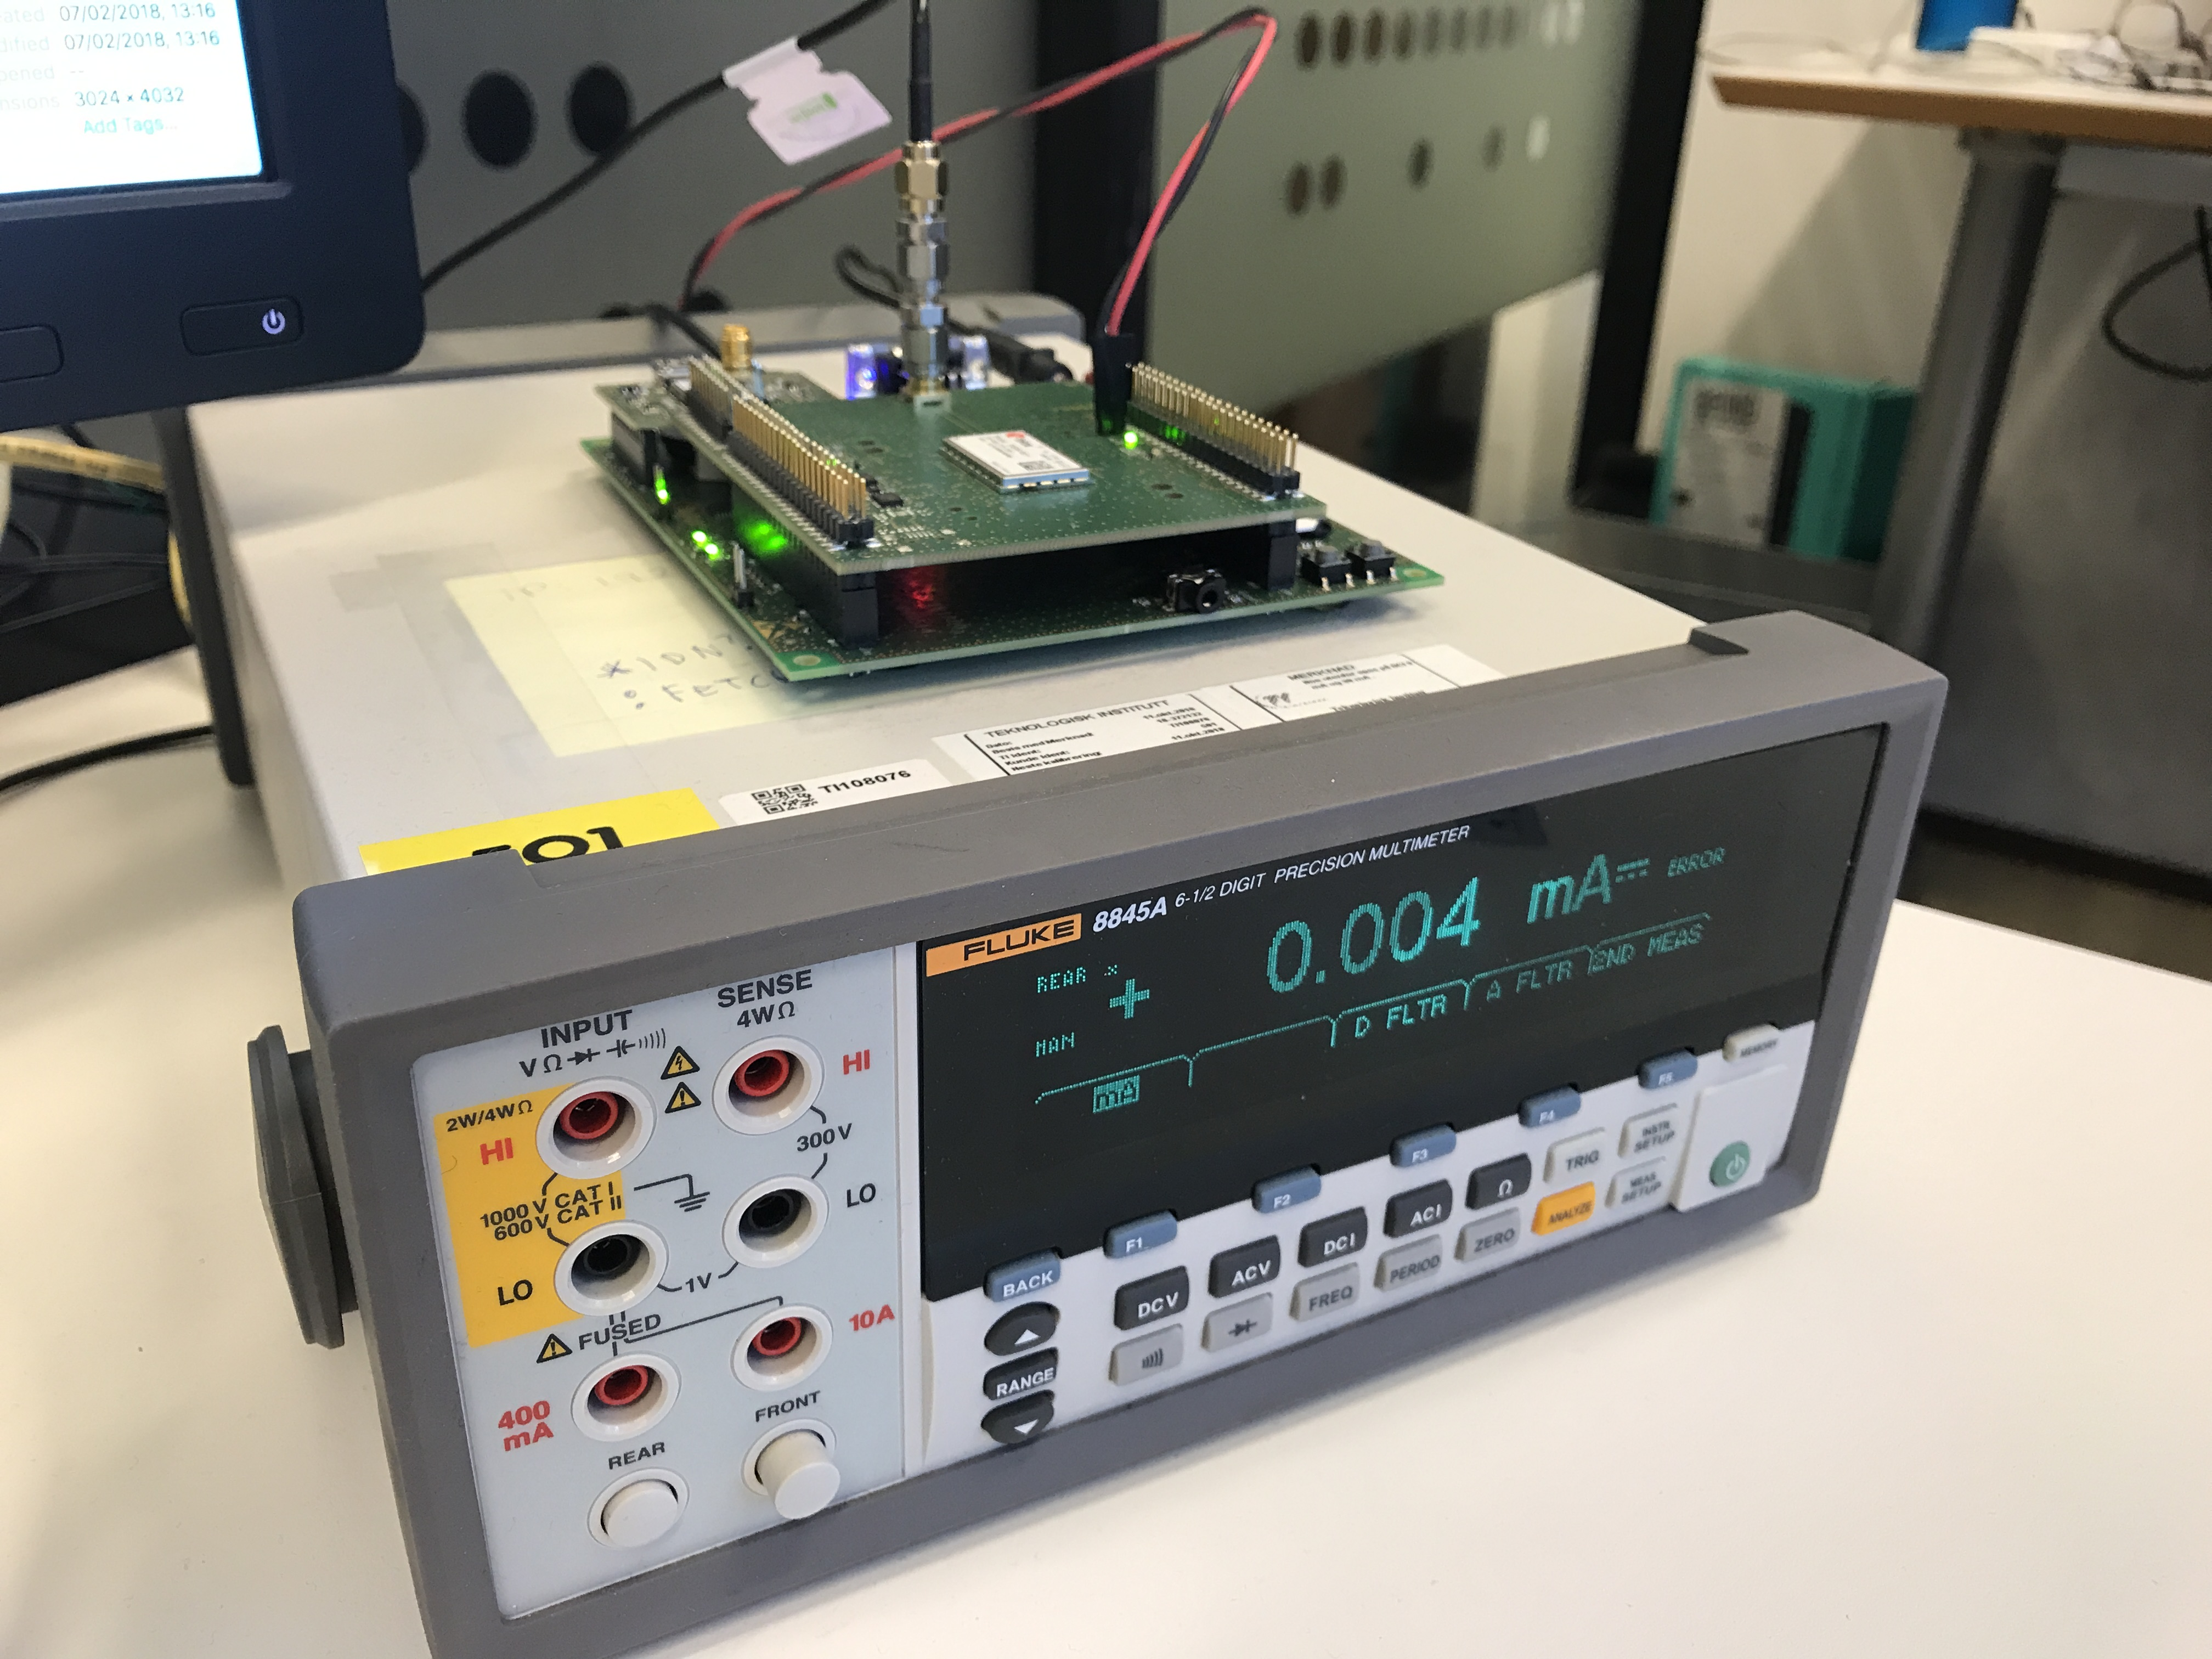
\includegraphics[width=12cm,height=8cm]{/Users/henninghakonsen/Dropbox/Masteroppgave/thesis/latex/images/uio_nbiot_setup.jpg}
  \caption{\acrshort{nb-iot} and multimeter setup}
  \label{pic:uio_nbiot_setup}
\end{figure}

\begin{figure}[H]
  \centering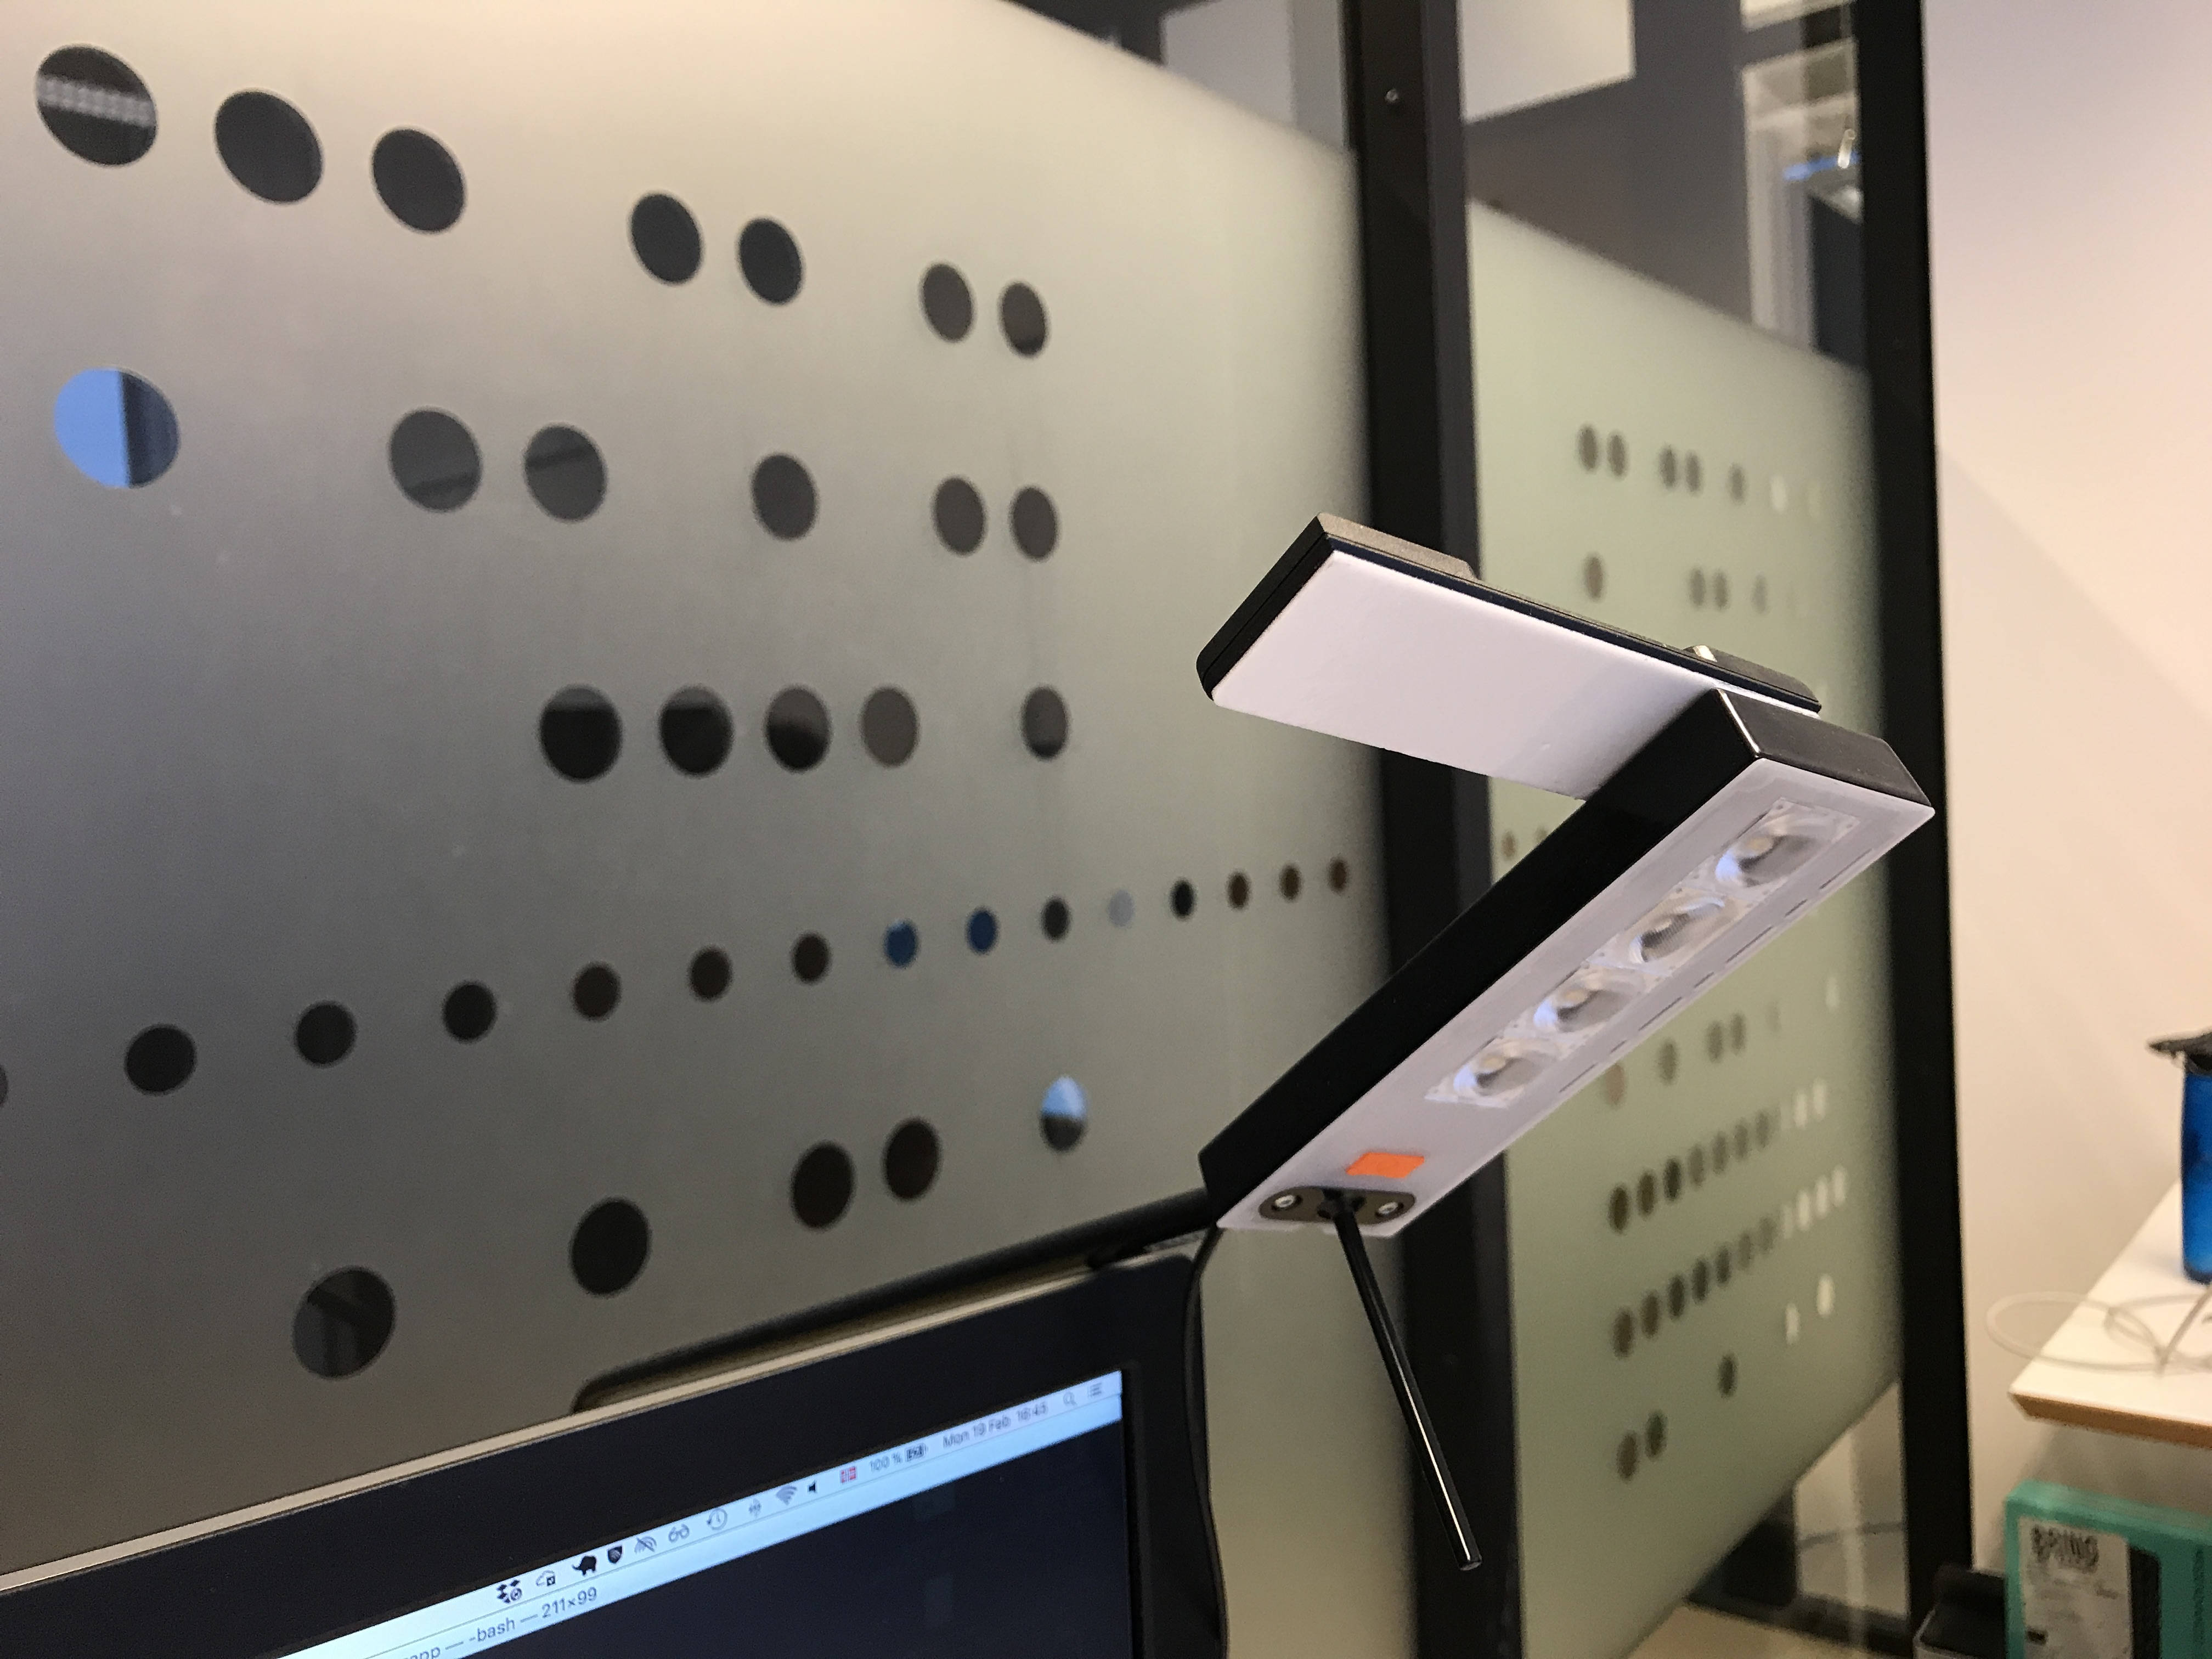
\includegraphics[width=12cm,height=8cm]{/Users/henninghakonsen/Dropbox/Masteroppgave/thesis/latex/images/antenna_position.jpg}
  \caption{\acrshort{nb-iot} antenna position}
  \label{pic:antenna_position}
\end{figure}

\subsection{Maps and distances} \label{ssection:mapsndistances}
\begin{figure}[H]
  \centering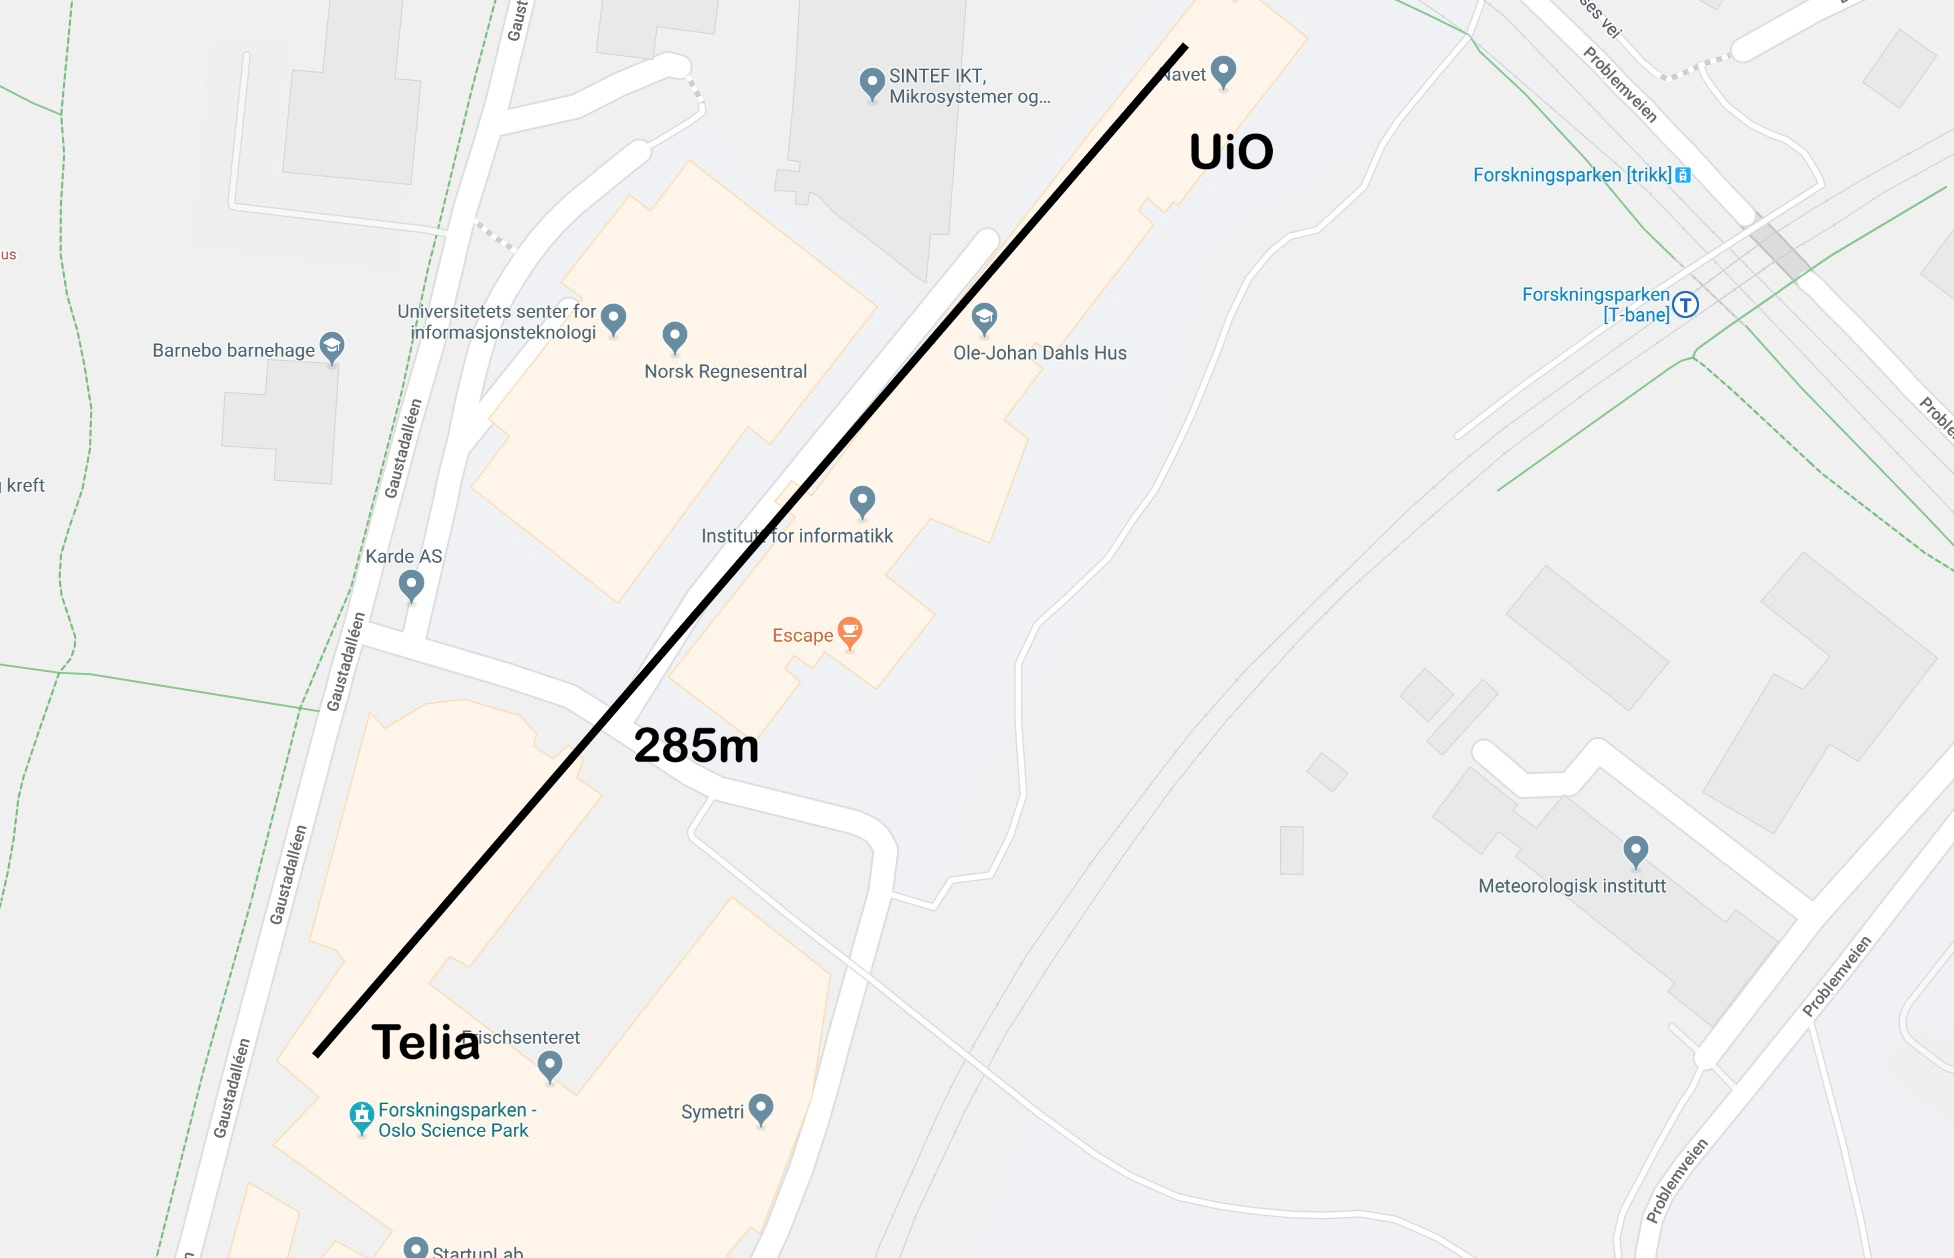
\includegraphics[width=\textwidth,height=0.4\textheight]{/Users/henninghakonsen/Dropbox/Masteroppgave/thesis/latex/images/map_uio}
  \caption{Map over IFI, UiO. We believe Telenor's cells are located close to Telia's. \cite{online:finnsenderen}}
  \label{figure:map_uio}
\end{figure}

\begin{figure}[H]
  \centering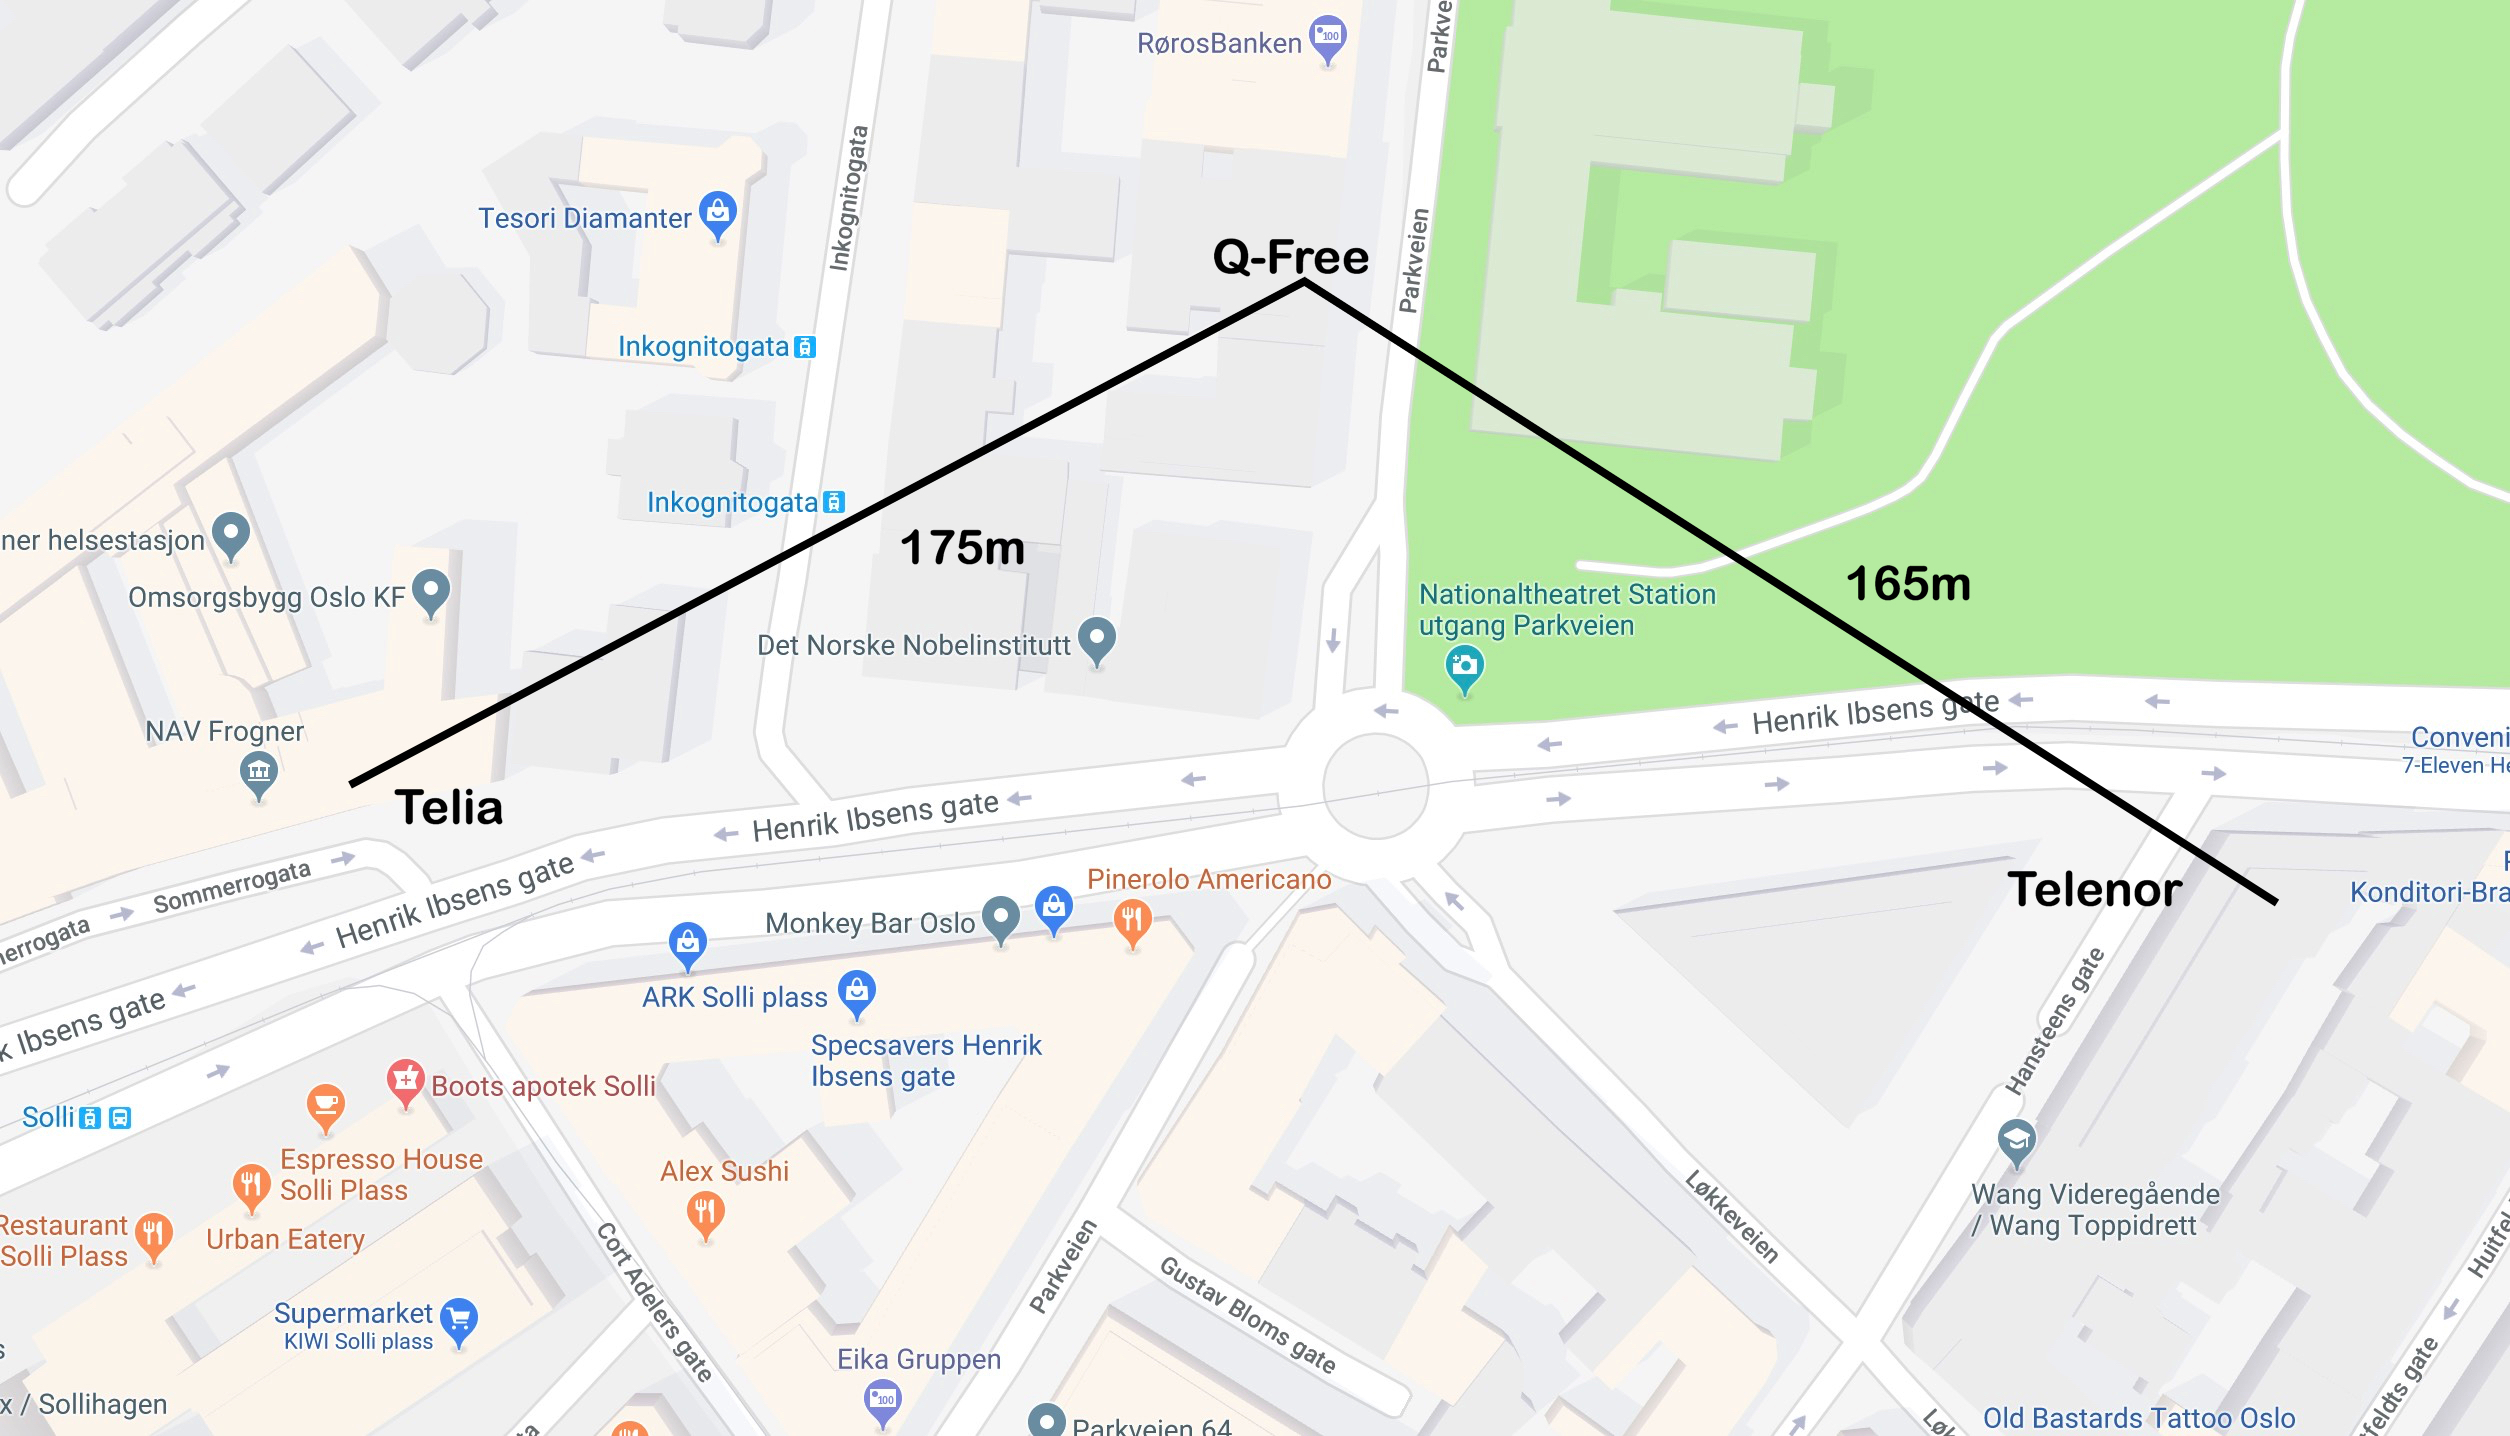
\includegraphics[width=\textwidth,height=0.4\textheight]{/Users/henninghakonsen/Dropbox/Masteroppgave/thesis/latex/images/map_qfree}
  \caption{Map over Q-Free.}
  \label{figure:map_qfree}
\end{figure}

\begin{figure}[H]
  \centering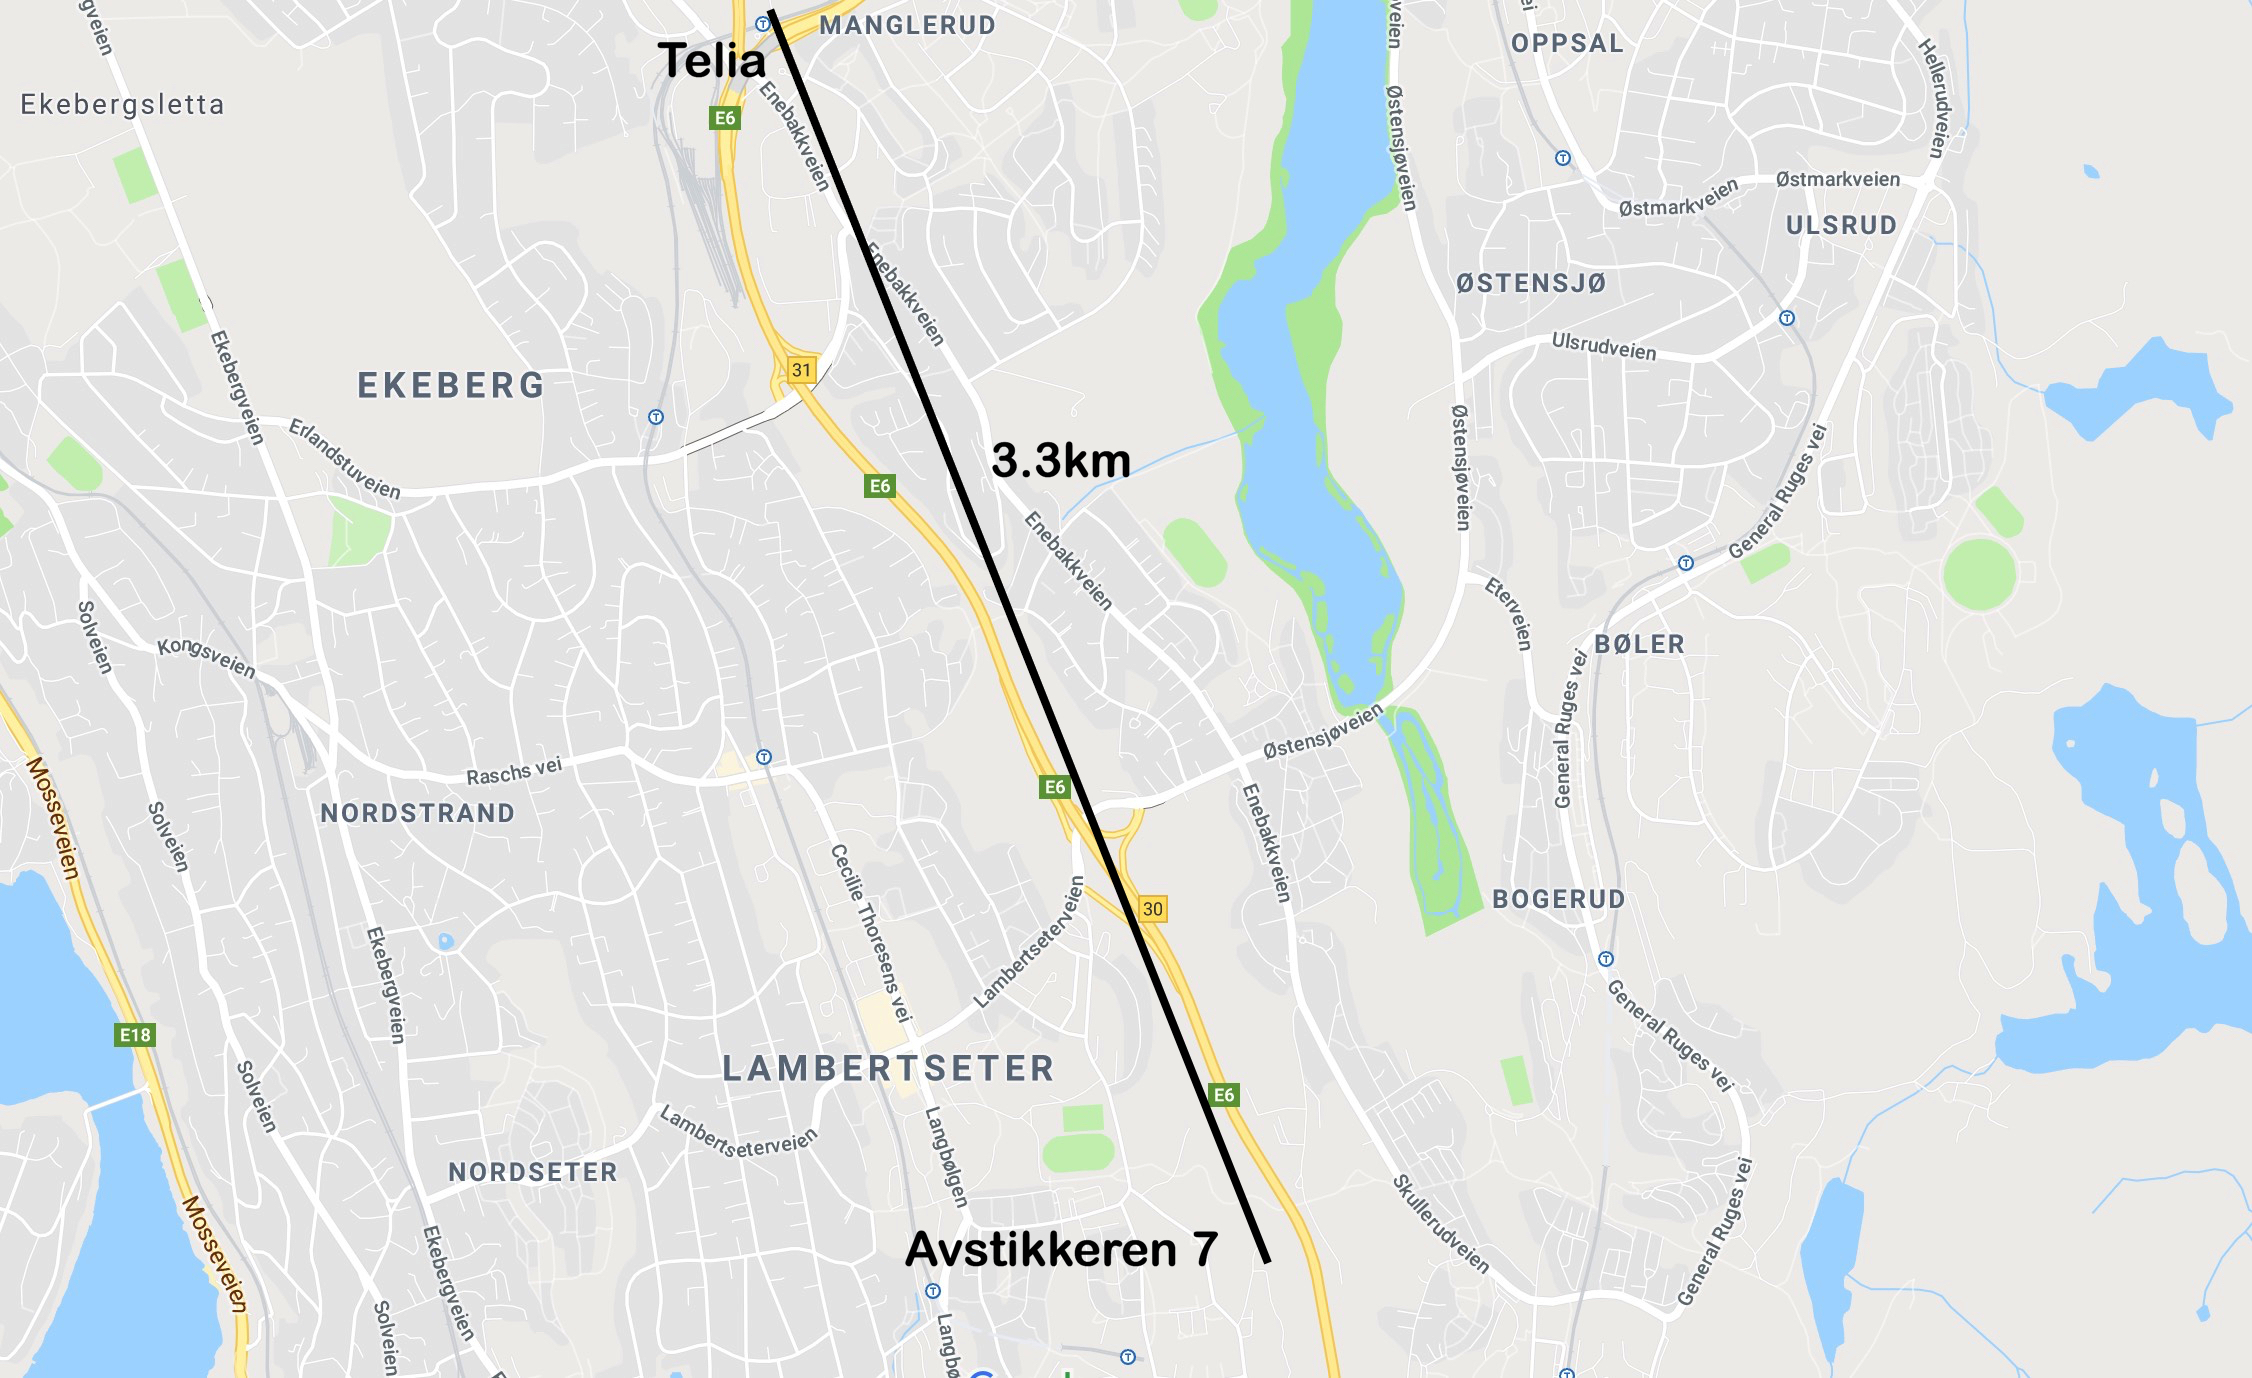
\includegraphics[width=\textwidth,height=0.4\textheight]{/Users/henninghakonsen/Dropbox/Masteroppgave/thesis/latex/images/map_avstikkeren}
  \caption{Map over Avstikkeren. The device did not manage to connect to Telenor's network at this location.}
  \label{figure:map_avstikkeren}
\end{figure}

\section{Devices} \label{ssection:devices}
We have used a set of devices to achieve the results and in the following subsections we will give you an introduction to the devices used and why they were necessary for our tests.

\subsection{Server}
To host our web application we applied for a server at UH-IaaS, which hosts servers for university projects. We received a well suited server with the necessary specifications suited for our appication. The server was at times unstable due to power outages, but no results were damaged due to the downtime. In section, \vref{chapter:webapp}, we will give a detailed description of the web application.

\subsection{\acrshort{nb-iot} development kit}
Q-Free received early 2018 a development kit for \acrshort{nb-iot} from the software company Ublox. This is a kit with a \acrshort{nb-iot} chip called SARA N2 from Neul and software from Ublox, see picture \vref{pic:nbiotdevkit}. The development kit enabled us to easily develop software for our tests which was crucial. The development kit was connected to a computer over USB and allowed us to send and receive data through the serial port of the chip. We used this setup for all our tests, which includes packet size, coverage, latency and general behavior of the network. We also used this setup for longer tests where we continuously send messages with a more practical frequency to the server. The computer will run different python programs to test the different features and for our long term tests we will send \textbf{AT+NUESTATS} to the application server so that we can process the information. In many cases we will also log test runs on the computer for detailed graphs of the behavior of the chip. The following subsection will give a detailed introduction to the chip we used.

\begin{figure}[ht]
  \centering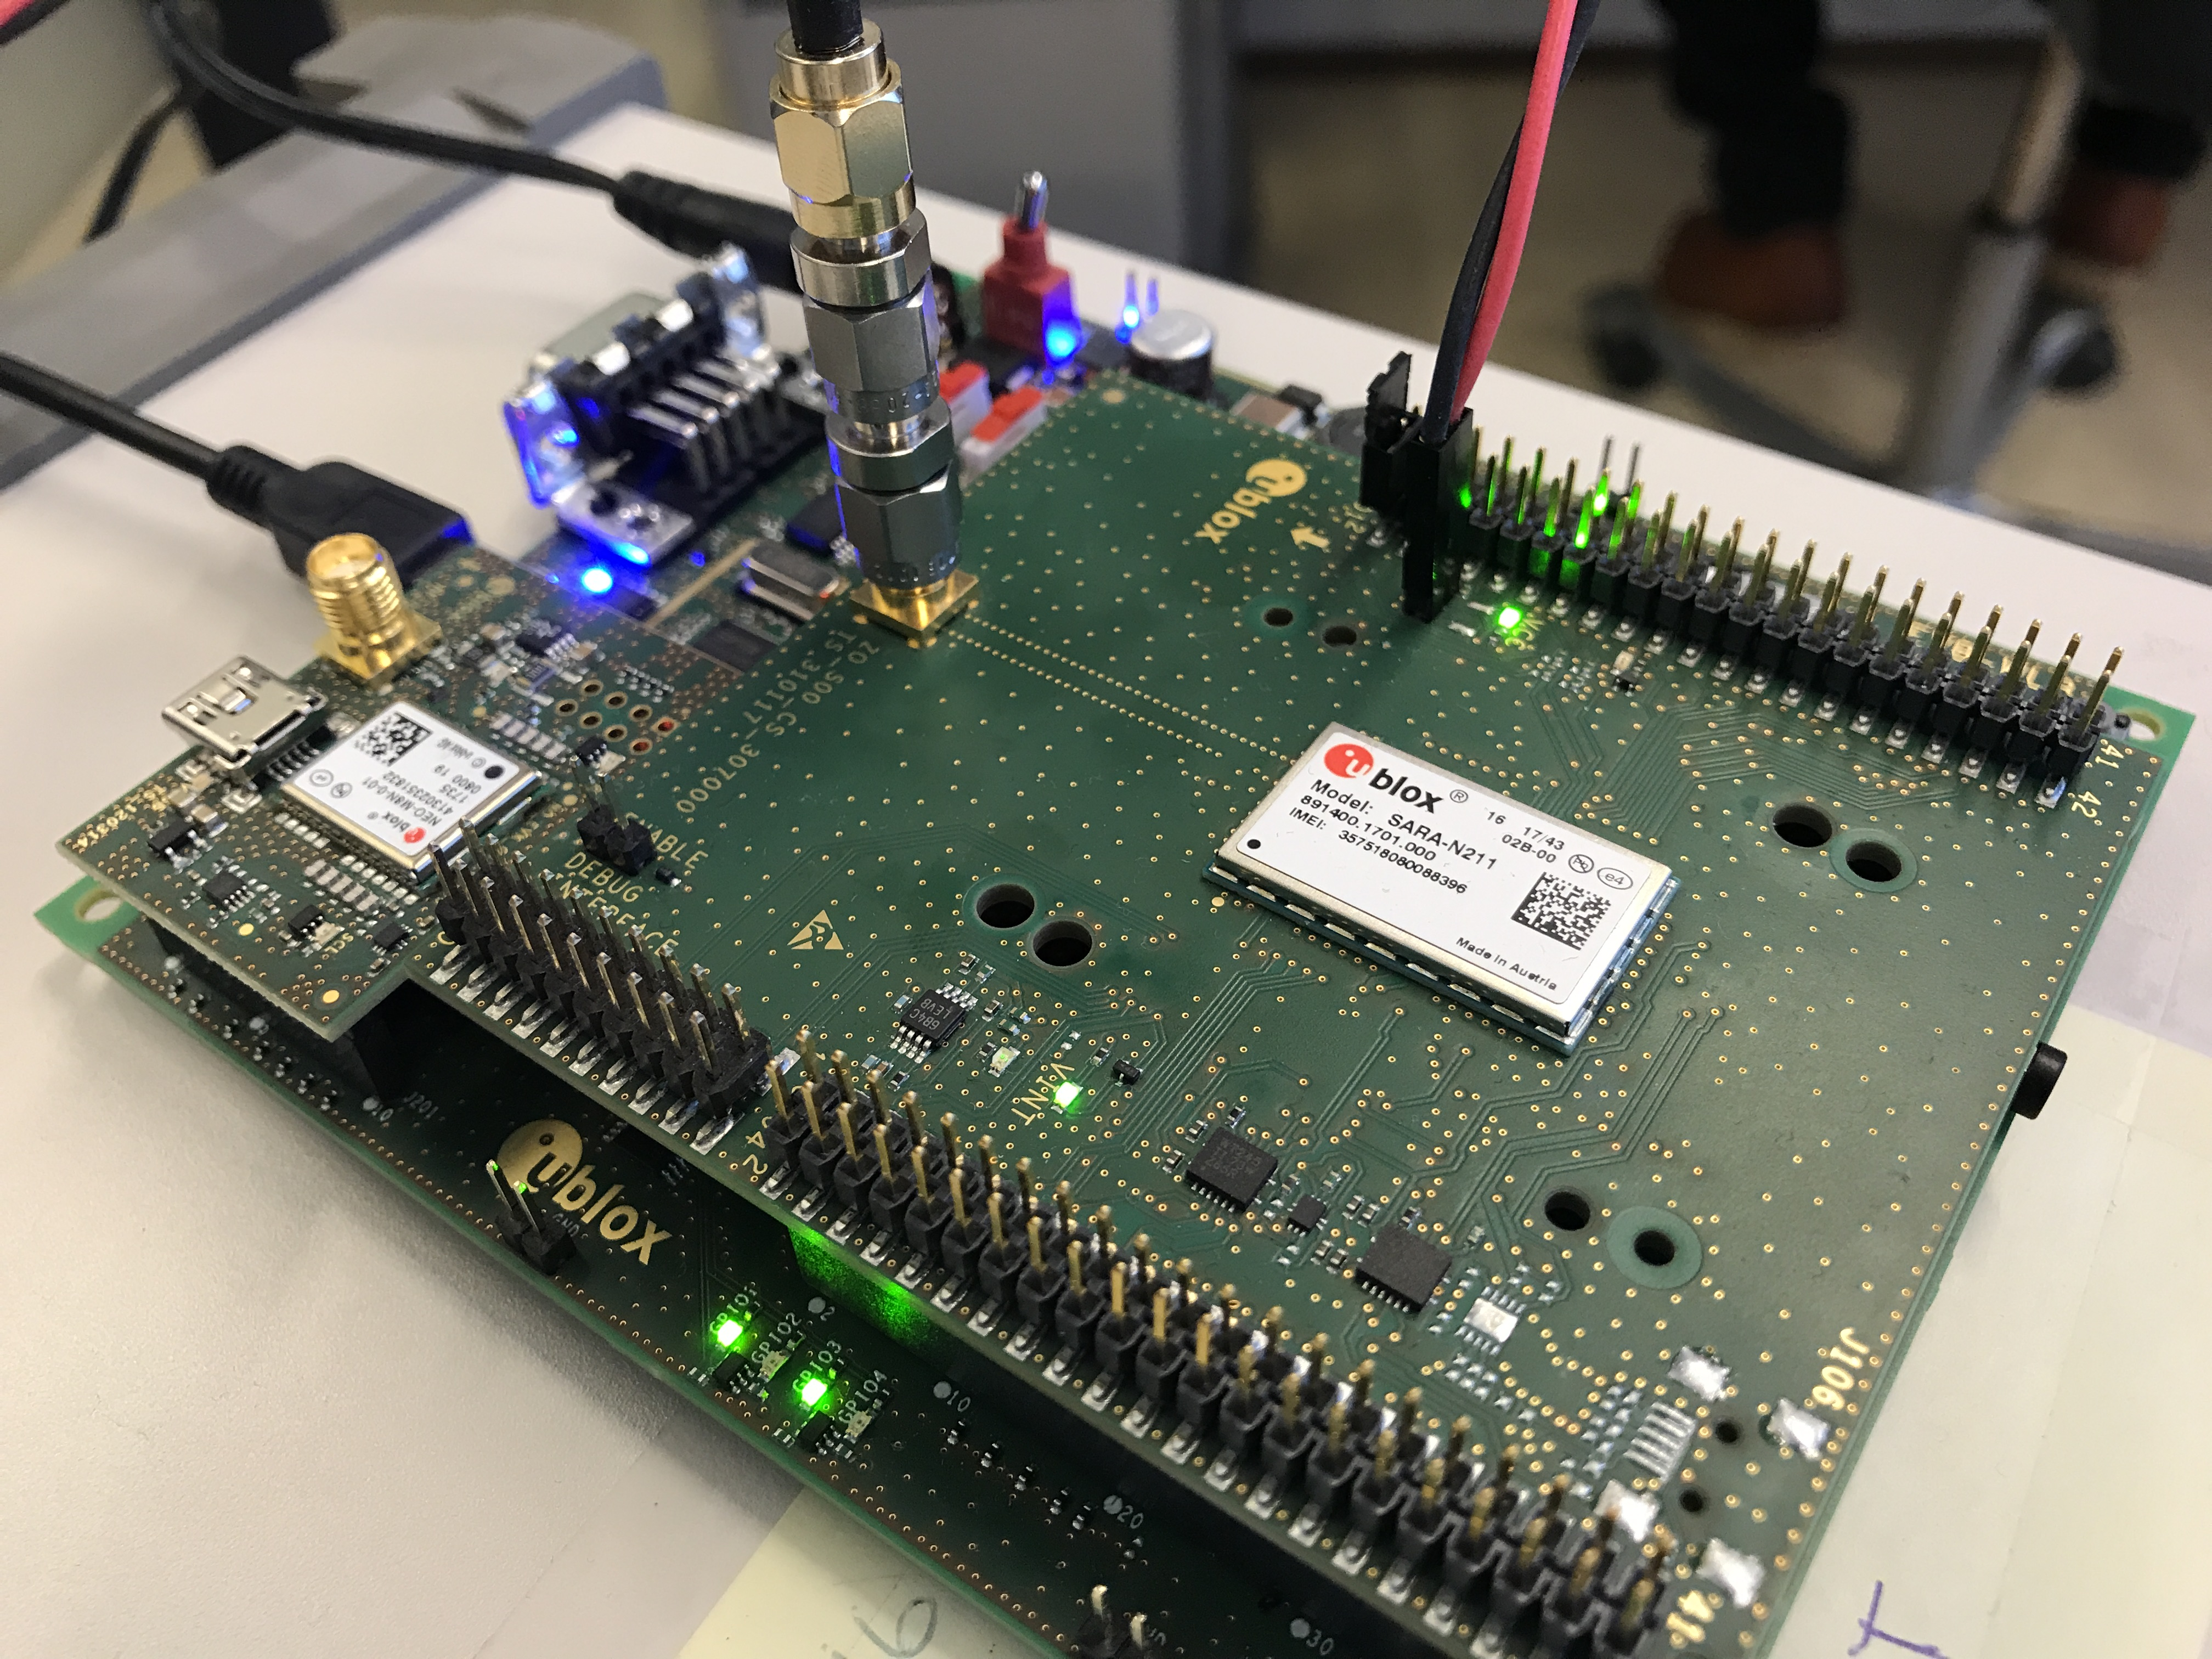
\includegraphics[width=12cm,height=8cm]{/Users/henninghakonsen/Dropbox/Masteroppgave/thesis/latex/images/nbiot_devkit.jpg}
  \caption{Ublox \acrshort{nb-iot} development kit. Here with both attenuators, which is a total of ${-30\acrshort{dbm}}$ signal loss.}
  \label{pic:nbiotdevkit}
\end{figure}

\subsubsection{Sara N2 Ublox chip} \label{section:thechip}
In section, \vref{paragraph:sensoroutline}, we looked at Q-Free's parking sensor, which houses an identical \acrshort{nb-iot} Ublox chip which will use for our tests. In this section we will look at the most essential modem commands for the \acrshort{nb-iot} chip. Modem commands are often referred to as AT-commands and we will use this notation throughout this paper. As mentioned in section, \vref{section:energysaving}, there are configurable timers in the network, as well as flags to keep in mind while developing software for low powered sensors. These parameters can be configured with AT-commands and has proven to give good results when taking power usage into consideration\footnote{We have only used the default timers in this paper}. In addition we will show you the AT-command for sending data, and how we intend to structure the data being sent.

In the following subsections we will give a brief introduction to the most important AT-commands taken from the AT Commands Manual for the \acrshort{nb-iot} chip \cite{atcommand:ubloxchip}.

\subsubsection{Monitoring - NUESTATS}
Monitoring is an important part of developing and a way to verify that your software is running as optimal as possible. In our case we wanted a way to monitor the performance of the \acrshort{nb-iot} chip, hence we wanted to take advantage of the precise statistics given from the command \textbf{AT+NUESTATS}. According to the specifications of \acrshort{nb-iot}, there are a number of interesting thresholds and \textbf{AT+NUESTATS} will give us most of this information. In table, \vref{table:nuestats}, you can see the output of the command.

\begin{table}[H]
\centering
\resizebox{\textwidth}{!}{%
\begin{tabular}{|l|m{10cm}|}
  \hline
  \textbf{Property} & \textbf{Description} \\ \hline
  Power & NB-IoT signal power expressed in tenth of dBm \\ \hline
  Total power & Total power within received bandwidth expressed in tenth of dBm \\ \hline
  Tx power & Transmit power expressed in tenth of dBm \\ \hline
  Tx time & Elapsed transmit time since last power on event expressed in milliseconds \\ \hline
  Rx time & Elapsed receive time since last power on event expressed in milliseconds \\ \hline
  Cell id & Physical ID of the cell providing service to the module \\ \hline
  \acrshort{ecl} & Last \acrshort{ecl} value \\ \hline
  \acrshort{snr} & Last \acrfull{snr} value \\ \hline
  \acrshort{earfcn} & Last \acrfull{earfcn} value \\ \hline
  \acrshort{pci} & Last \acrfull{pci} value \\ \hline
  \acrshort{rsrq} & Last \acrfull{rsrq} value \\ \hline
\end{tabular}%
}
\caption{\textbf{NUESTATS} command}
\label{table:nuestats}
\end{table}

We believe that using \textbf{AT+NUESTATS} will give us accurate results. In addition we will use a high precision multimeter to monitor the current through the \acrshort{nb-iot} chip.

\subsubsection{Time - CCLK}
Time is another tool we often use for developing software. We want to know how long a process endures, and in our case we want to monitor the latency of a send operation from the sensor to the server. With the AT-command \textbf{AT+CCLK?} we can read the time from the chip. This time is kept in sync with the network and stored in the \acrshort{mt}. The read operation returns a string with the time in the following format "yy/MM/dd,hh:mm:ss+TZ", where the characters represent, year, month, day, hours, minutes, seconds and time zone. However, we soon realised that the internal clock wsa not very good and after the device had been operational for a day the internal clock would be skewed and the latency results were not accurate. We will elaborate in more detail about this problem in section, \vref{section:deviations}, but our suspicion is that the clock is not updated very often and with an imprecise internal clock the time will be wrong. As we were perfoming all tests with a computer connected to the development kit we started using the clock of the machine connected to the kit and send this timestamp to the server. This did not only give us a more updated clock, but the timestamp also included milliseconds which gave the result higher precision.

\subsubsection{\acrshort{edrx} settings - CEDRXS}
In section, \vref{ssection:edrx}, we explained how \acrshort{edrx} works and how we can configure the \acrshort{ue}. With the AT-command \textbf{AT+CEDRXS} we are able to define how \acrshort{edrx} is performed on the \acrshort{ue}. We can for example issue this AT-command, \textbf{AT+CEDRXS: 1, 5, "0101"}, to put the \acrshort{ue} into \acrshort{edrx} mode with cycle length of 163.84 seconds\footnote{This is the factory-programmed \acrshort{edrx} timer for SARA N2 chip}.

\subsubsection{\acrshort{psm} settings - CPSMS}
We can also define how \acrshort{psm} is used on the \acrshort{ue}. We can enable \acrshort{psm}, and set the timer \acrfull{T3412}\footnote{The factory-programmed value of \acrshort{T3412} is 54 m.\cite{atcommand:ubloxchip}} with this command. If \acrshort{psm} is enabled, the device will enter deep sleep after expiry of the timer \acrfull{T3324}\footnote{The factory-programmed value of \acrshort{T3324} is 60 s.\cite{atcommand:ubloxchip}}.

\subsubsection{Create socket - NSOCR}
Opens a port on the \acrshort{ue}, which enables data transfer on the given port. In our application we will open an \acrshort{udp} socket on a port. The port used can be a number between 0-65535, except for 5683 since this is used by the chip to send \acrshort{coap} messages. The command returns a socket number which will be used for trailing send(NSOSTF) commands.

\subsubsection{Send command with flags - NSOSTF}
This AT-command is used to send \acrshort{udp} packets on a given port with a specified flag. The command takes a set of parameters and the data in hexadecimal format. The parameters are, socket number(given by the AT-command NSOCR), remote IP address, remote port, flag, data length and actual data. The flag can be used to specify the behavior of the \acrshort{ue} after the data has been transmitted, see table, \vref{table:flag}, for details.

\begin{table}[H]
\centering
\resizebox{\textwidth}{!}{%
\begin{tabular}{|l|m{10cm}|}
  \hline
  \textbf{Mode} & \textbf{Description} \\ \hline
  0 & No flags are set \\ \hline
  1 & Send message with high priority \\ \hline
  2 & Indicates \acrshort{rai}. This mode will put the \acrshort{ue} into \acrshort{psm} mode directly after transmitting data. Meaning less time in power heavy modes. \\ \hline
  3 & Indicate release after next message has been replied to. \\ \hline
\end{tabular}%
}
\caption{Transmit flags}
\label{table:flag}
\end{table}

The data we transmit towards our server adds an additional \acrshort{coap} header followed by the actual data. We decided to do this to reduce logic on the server and create the environment similar to a real world application.

\subsubsection{Signaling connection status - CSCON}
We can verify the connection status of the \acrshort{ue} with the command \textbf{AT+CSCON?}. If the reply is 1 this means that the \acrshort{ue} is in RRC connected mode and is able to send and receive packets. If the reply is 0 this means that the \acrshort{ue} is in idle mode, hence the device is inactive. Note that this does not mean that the device is in \acrshort{psm} mode. This only occours after the configured \acrshort{T3324} timer expires.

\subsubsection{Network registration status - CEREG}
We can verify the network registration status of the \acrshort{ue} with the command AT+CEREG. This command is a very useful command for any application which wants to check if the \acrshort{ue} is still connected to the network.

\subsubsection{\acrshort{psm} status - NPSMR}
Gives us the status of \acrshort{psm} on the device. It will return \textbf{1,1} if the device is in \acrshort{psm} mode which means that the power usage is very low \footnote{${~3\mu A}$ in deep sleep mode}.

\subsection{Fluke precision multimeter}
Q-Free owns a precision multimeter which we used to measure the current through the \acrshort{nb-iot} chip. With the multimeter we managed to pinpoint different stages of the chip. In addition we added corresponding statistics from \textbf{AT+NUESTATS} which increased the precision. As sketched in figure, \vref{figure:labsetup}, we connected the multimeter to the computer using an ethernet cable, enabling us to fetch readings from the device.
Depending on the selected precision of the measurements we collected between 30-300 samples per second. The most detailed tests required high sample rate, while we used lower precision measurements on longer tests. The device responded on commands much like a \acrfull{repl}, where you issue a request with a command and the device will respond with an answer. In table, \vref{table:fluke_commands}, you can see the commands we used and a short description related to them.

\begin{table}[H]
\centering
\resizebox{\textwidth}{!}{%
\begin{tabular}{|l|m{10cm}|}
  \hline
  \textbf{Command} & \textbf{Description} \\ \hline
  :INIT & Clears old readings \\ \hline
  :FETCH? & Fetches all readings from the device. The response is a long string with numbers divided with "," \\ \hline
\end{tabular}%
}
\caption{Fluke commands}
\label{table:fluke_commands}
\end{table}

\section{Software}
Writing software which should produce a set of results is hard, particularly when you don't know the expected results. We developed many test programs with a specific setup(see figure, \vref{figure:labsetup}, for an overview) as well as an web application to give us the knowledge and experience to give a precise report about the status of \acrshort{nb-iot} the spring of 2018. A thing we learned during the testing phase is that the output format often changed and since our programs outputs data which is already processed it meant that we needed to reperform some tests. In hindsight it would be better to capture the raw data and develop a program which generated graphs based on the data. However, we are satisfied with the end result and you will see many of the generated graphs in section, \vref{section:testing}.

\begin{figure}[ht]
  \centering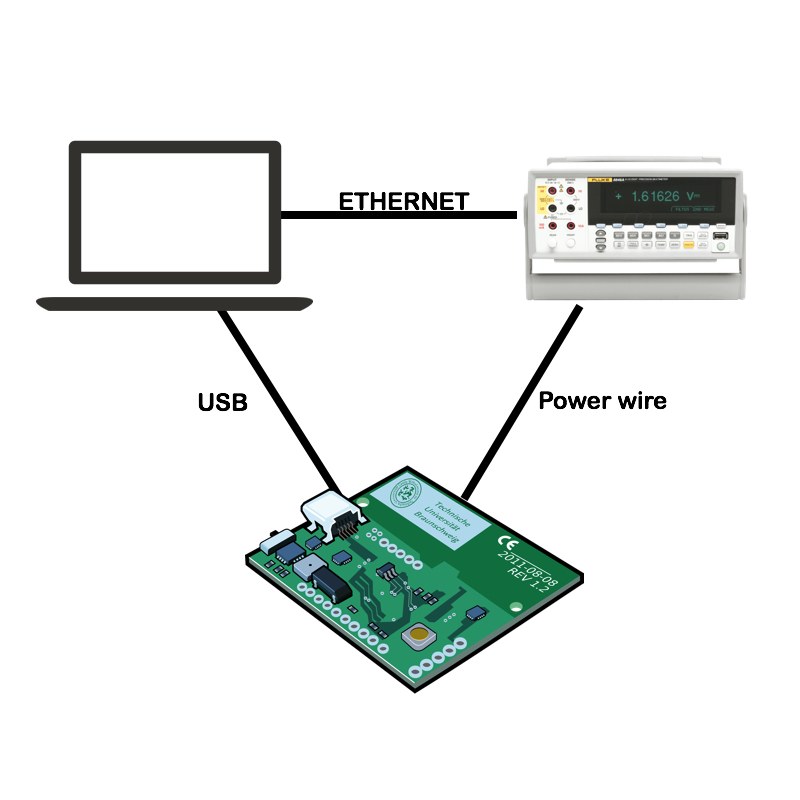
\includegraphics[width=10cm,height=10cm]{/Users/henninghakonsen/Dropbox/Masteroppgave/thesis/latex/images/labsetup.jpg}
  \caption{Lab setup \cite{pcpng35052:online} \cite{fluke88435:online} \cite{ingagrue31:online}}
  \label{figure:labsetup}
\end{figure}

We wrote test features for the development kit using python with a connection between the program and the serial port. We configured the device to make sure that everything is according to our setup, see code \vref{code:modem}.

\begin{lstlisting}[caption={Development kit initiation},label={code:modem},language=Python]
  uart_modem = serial.Serial(<serial port>, 9600, timeout = 0)
  uart_modem.close()
  uart_modem.open()
  uart_modem.flushInput()
  uart_modem.flushOutput()
\end{lstlisting}

We started experimenting with different AT commands and created small programs to test the functionality of the chip and the connection towards the server. We created a simple program which sent \textbf{AT+NUESTATS} to the application server and went on transforming this program to helper methods we could use later on. A sample packet with a COAP header would look something like the example, \vref{samplecommand}, where the payload is converted to hexadecimal. We used some time creating the correct COAP packet for the server to accept it as a COAP packet. If you don't want to use COAP you can simply fill the payload with data without the COAP header, but this means that you are missing the features of COAP which could be beneficial for your application. Dropping the COAP header means that you are sending a pure \acrshort{udp} packet through the network and it is harder to verify the packet when it is received on an eventual application server.

\begin{lstlisting}[caption={Sample transmit 158.39.77.97:5683, 88 bytes},label={samplecommand},language=Python]
  AT+NSOSTF=0,"158.39.77.97",5683,0x0,88,"500230
  30B131112AFF2D313039365F2D313034325F3233305F39
  3732315F37363838305F33343433393435325F315F3132
  335F363235325F39385F2D3130385F31382F30322F3139
  2C31363A31363A35362B30305F31325F"
\end{lstlisting}

We proceeded working on communication towards the multimeter, which was quite easy. The multimeter was given an \acrshort{ip} address which was related to the \acrshort{ip} address of the connected machine. Creating a socket to this IP address in python and connecting to it was simple. The test programs starts off by clearing all buffers with \textbf{:INIT} and then fetch for data on a regular interval with \textbf{:FETCH?; :INIT}. With each reading we converted the string into a list of numbers which we appended to a global list of readings. We found that fetching for new data every 5th second was a good tradeoff between fetching all the time and very rare. We added these functions to the helper file, \textbf{nbiot\_labtest\_helpers.py}, and went on writing a couple of programs to monitor the behavior of the chip.

In the following sub section we have included some documentation on the most essential test programs. In the following chapter, \vref{chapter:webapp}, we will describe the web application.

\subsection{Test programs}
\paragraph{\textbf{at\_command\_test.py}} is a program well suited for testing different AT commands which is necessary to explore and research how the device handles different features. The program is like a \acrshort{repl} and requests an optional message and a command. If a message is supplied the program assumes that the request is a send command. If not the command is handled and the respons is printed in the terminal. Note that this program is written in python2 while the other programs expect python3 to execute. See \href{https://github.com/henninghaakonsen/thesis/blob/master/code/at_command_test.py}{AT command \acrshort{repl}}\cite{code:atcommand} for complete code.

\paragraph{\textbf{nbiot\_labtest.py}} continuously transmits packets over \acrshort{nb-iot} - either status packets towards the server or random data of different sizes. It enabled us to test different scenarios and log the results in a representable way with graphs. The program takes in a list of parameters described in table, \vref{table:labtestparameters}.

\begin{table}[H]
\centering
\resizebox{\textwidth}{!}{%
\begin{tabular}{|l|m{10cm}|}
  \hline
  \textbf{Parameter} & \textbf{Description} \\ \hline
  -id & ID which you want to POST towards the server. Default: 0 \\ \hline
  -gn & Output graph name. The supplied name will lead the heading, followed by a list of the rest of the parameters. \\ \hline
  -d & Set the desired delay between each iteration. Default: 5 \\ \hline
  -i & Set the desired iterations. Default: -1 which means that the program will loop until the user presses ctrl+c \\ \hline
  -b & Set the desired length of the payload in bytes. If 0 is requested, statistics from \textbf{NUESTATS} will be sent to server. Default: 100 \\ \hline
  -r & Set \acrshort{rai}. Default: false \\ \hline
  -l & Set device logging. Default: false \\ \hline
  -rb & Set test to reboot \acrshort{nb-iot} chip directly after execution. Default: false \\ \hline
\end{tabular}%
}
\caption{\textbf{nbiot\_labtest.py} parameters. See \href{https://github.com/henninghaakonsen/thesis/blob/master/code/nbiot_labtest.py}{\acrshort{nb-iot} labtest}\cite{code:nbiotlabtest} for complete code}
\label{table:labtestparameters}
\end{table}

To get more stable tests and to automate the process we added logic to perform a set of tests when starting the program. If byte size is not given to the program the execution will perform 4 tests on 50, 100, 200 and 512 bytes. Those 4 tests are a combination of logging and \acrshort{rai}.

For each iteration the program sends a message towards the server, followed by a period of logging. If logging is enabled the program fetches information from the chip with \textbf{NUESTATS} and three other commands - \textbf{AT+NPSMR?}, \textbf{AT+CSCON?} and \textbf{AT+CEREG?}. From \textbf{NUESTATS} we retrieve information about transmit and receive time, transmit power, \acrshort{ecl} level and signal power. We choose these parameters because they give us good information by themselves, as well as they combined gives a good indication of what the chip is doing at any time. These results were logged approximately four times per second - limited to the speed of the serial bus between the computer and the development kit. Every fifth second we also fetch stored information from the precision multimeter. Depending on the configured precision of the multimeter we logged 50-400 samples per second which we in turn could correlate to the logged information from the chip. With all results the program produces a set of graphs which we will use for analysis of the network and the chip.

Because we were not able to collect the timestamp of each measurement of the multimeter we had to flatten the result and apply a timestamp to each measurement. This means that we assume that the interval is equal. When looking at the figures in section, \vref{section:detailedtest}, the power graphs are mostly linked to the results created from \textbf{NUESTATS}, but often one or two seconds subsequent of the other graphs.

\textbf{Graphs generated:}
\begin{itemize}
  \item Receive: Shows the percentage of how much time the device were receiving compared to the actual interval.
  \item Transmit: Shows the percentage of how much time the device were transmitting compared to the actual interval. Both receive and transmit scales are incorrect, and should actually be multiplied with 100, so that 1 actually is 100\%.
  \item Transmit power: Shows the transmit power of the device.
  \item Coverage: Shows the coverage of the device.
  \item \acrshort{ecl} level: shows which coverage mode the device is currently in.
  \item \acrshort{psm}: Shows the status of \acrshort{psm}.
  \item RRC state: Shows the RRC state.
  \item Registration status: Shows the registration status of the chip. 1 is connected, 4 is unknown and 5 is searching for network.
  \item Power usage: Shows the current through the chip in \acrshort{ma}.
\end{itemize}

Based on the average current over the time of the test we can also calculate total power usage. With the average current we can convert this to \acrshort{mwh} and convert this to \acrshort{mws} and multiply the result with the time of the test. This is an example from \href{http://158.39.77.97:9000/\#/results/UiO\_TELIA\_5.02\_precision\_2018-03-16\_1\_0x2\_60\_1\_512}{webapp} \cite{webapp:powerexample}: ${( (9.2089 \acrshort{ma} * 3.3V) / 60 / 60 ) * 60 = ~0.5064 \acrshort{mwh}}$. With this information we can show the difference in power usage with different scenarios and try to use the results to outline the lifetime of a device under different kinds of environments.

\paragraph{\textbf{power\_calculator.py}} calculates the power consumption over a given period from one of the test results from the short term tests. We needed this tool to figure out how much power specific parts of the transmit used. It extracts all power measurements, in \acrshort{ma}, between two timestamps and calculates the average current, multiplying this with the time delta between the two timestamps supplied. The program takes in a list of parameters described in table, \vref{table:powercalculator}.

\begin{table}[H]
\centering
\resizebox{\textwidth}{!}{%
\begin{tabular}{|l|m{10cm}|}
  \hline
  \textbf{Parameter} & \textbf{Description} \\ \hline
  -f & File name. Must be from short term test and have .html format \\ \hline
  -s & Start time \\ \hline
  -e & End time \\ \hline
\end{tabular}%
}
\caption{\textbf{power\_calculator.py} parameters. See \href{https://github.com/henninghaakonsen/thesis/blob/master/code/power_calculator.py}{power calculator}\cite{code:powercalc} for complete code}
\label{table:powercalculator}
\end{table}

\paragraph{\textbf{nbiot\_labtest\_details.py}} tests different packet sizes. The program transmits 6 packets with different packet sizes\footnote{25, 50, 100, 200, 400 and 512 bytes} a given number of times. After the given iterations are processed the program produces two graphs, one with all recordings and one with normalized data\footnote{We have choosen to include average, sum, min and max values for each packet size}. The program takes in a list of parameters described in table, \vref{table:nbiotdetails}.

\begin{table}[H]
\centering
\resizebox{\textwidth}{!}{%
\begin{tabular}{|l|m{10cm}|}
  \hline
  \textbf{Parameter} & \textbf{Description} \\ \hline
  -id & ID which you want to POST towards the server. Default: 0 \\ \hline
  -gn & Output graph name. The supplied name will lead the heading, followed by a list of the rest of the parameters. \\ \hline
  -d & Set the desired delay between each iteration. Default: 5 \\ \hline
  -i & Set the desired iterations. Default: 1 \\ \hline
  -r & Set \acrshort{rai}. Default: false \\ \hline
\end{tabular}%
}
\caption{\textbf{nbiot\_labtest\_details.py} parameters. See \href{https://github.com/henninghaakonsen/thesis/blob/master/code/nbiot_labtest_details.py}{\acrshort{nb-iot} details}\cite{code:nbiotdetails} for complete code}
\label{table:nbiotdetails}
\end{table}

\chapter{The web application} \label{chapter:webapp}
In order to collect data we needed a web server and we needed to consider a few things, what should be included in the server, which platform should the server run on and where should the server be located. At the same time it was important to think about how the data would be used. The simple solution would be to collect the data and import it into an excel document for analysis. However, there are approximately eighteen thousand elements in the database, and maintaining and keeping track of this data in an excel document would not suffice for an effective analyzation of the data after the test. We decided to implement a web app to display information about the sensors. This web app can display latency, coverage and power related data about each sensor as well. In section, \vref{section:challenges}, we mentioned that we gained most knowledge from the short term test. However, we gained most of the practical knowledge from results coming into the web application and we would not perform the kind of tests which gave the most interesting results without the web application.

In the following sections we will discuss the implementation of the server and the web app.

\section{Backend: Node.js}
We decided to use node.js for what would become the backend of the server. Node.js is a new and modern way to create simple REST APIs. A REST API follows a set of rules to make it robust and stateless. It also should include all CRUD operations(create, read, update and delete) and should use the appropriate request method, such as POST, GET, PUT and DELETE. A big difference from standard backend programming is that Node.js uses javascript as programming language. Even though javascript is not the cleanest programming language it is efficient and the codebase is kept low. In addition node.js takes advantage of using \acrfull{npm}. \acrshort{npm} offers packages for all applications, both frontend and backend, and we will discuss some of the packages used in the server.

The server hosts multiple API endpoints. The most important are of course collecting data and retrieving data. The database contains a lot of data collected from different tests and it would require a lot of rendering to do analysis on the client side. We decided to analyze the data at specific intervals so that the client would simple display the data. We will describe the analysis and data which is displayed in section, \vref{ssection:analysis}.

\subsection{The database}
There are multiple ways to store data and there is always a trade off when choosing the platform. PostgreSQL is a great example of a database which is fast and reliable, but it can be complicated to set up and it is SQL driven which means all data has to fit into a pre-defined configuration. Since this project is small and the data could potentially changed during the test phase, we choose to use a NoSQL database. There are many good tools for storing data in a NoSQL database. ArangoDB and MongoDB are the most commonly used databases and both works well with Node.js. ArangoDB is often used for geo specific tasks and mongoDB was a bit easier to use, so we decided to use mongoDB for our data storage. In subsection, \vref{subparagraph:mongodb}, we will explain how we used mongoDB for our implementation.

\section{JavaScript packages for the server}
We used different packages from \acrfull{npm} to include certain features on our web server. By including quality packages our servers logic and size is kept low and we can focus on the data. In the following subsections we will give a short introduction to the most important packages used when developing the web server.

\subsubsection{Express}
Express is a fast and robust package for handling routes and offers nice APIs for listening on specific ports and so forth. In the following code example, \ref{code:express}, you can see the base setup for making your server handle requests. The port is set with a combination of the processes port and user specific port selection. The reason why this might be useful is if your server is hosted on a payed server which might be deployed on different IP and port for each deploy. With this implementation you won't need to consider this. In the example you can see a GET for a specific path, however you can also redirect all routes to a separate file for cleaner code. The last thing we need to do is to listen for incoming requests on the specific port. Now express will handle all request with an event loop.

\begin{lstlisting}[caption={Base express setup},label={code:express},language=JavaScript]
// express setup
const server = express();
const port = process.env.PORT || 8020;

server.get('/', function (req, res) {
  res.send('Hello World')
})

server.listen(port, () => {
  console.log(`app started on`, port);
});
\end{lstlisting}

\subparagraph{\acrfull{coap}} is a simple network protocol and offers request like HTTP, but without all the overhead. Coap is designed for low powered devices and will be used for our tests. I have used node-coap package for including \acrshort{coap} support on the server. Since the protocol is simple, we need to handle the request a bit different. The following code example, \vref{code:coap}, shows a simple node-coap setup.

\begin{lstlisting}[caption={Base \acrshort{coap} setup},label={code:coap},language=JavaScript]
var coap = require('coap')
var coap_server = coap.createServer()

coap_server.listen(port, () => {
    logger.log("info", `Worker ${process.pid} started coap server on ` + port);
})

// All request is handled by this function. It is not possible to request a specific url path
coap_server.on('request', function(req, res) {
    // Payload of the request is a byte stream. Parse the stream and handle the data
    var data = JSON.parse(req.payload.toString());
})
\end{lstlisting}

\subsection{Cluster}
With this simple setup all request will be handled by one thread by express as Node.js is single threaded. However with a package called cluster we can handle several request asynchronous. It is based on web workers which are an abstraction for processes in Node.js.
The following code example, \vref{code:cluster}, shows how you can enable multiple processes to handle your request to improve efficiency on your server. The cluster package offers a set of functions, so the first thing we do is to verify which worker is master. The master then forks a number of processes which then will request the path '/' and listen on the specified port. To avoid that all workers handle every request, cluster passes request in turn to the workers, normally in round robin fashion where worker 1 gets the first request, worker 2 the next and this goes on in a loop. Since the server will run over a long time, we need to handle workers which dies. The master process will pickup workers which die and respawn processes so that the server can continue processing requests.

Since the server basically puts everything on hold while analyzing the data we needed a way to handle request at the same time. The cluster package enables the server to handle incoming request as the analysis is ongoing.

\begin{lstlisting}[caption={Express setup with cluster},label={code:cluster},language=JavaScript]
const server = express();
const port = process.env.PORT || 8020;

const cluster = require('cluster');
const numCPUs = require('os').cpus().length;

if (cluster.isMaster) {
    console.log(`Master ${process.pid} is running`);

    // Fork workers.
    for (let i = 0; i < numCPUs; i++) {
      cluster.fork();
    }

    // Respawn workers on exit
    cluster.on('exit', (worker, code, signal) => {
      console.log(`worker ${worker.process.pid} died`);
      cluster.fork();
    });
} else {
    server.get('/', function (req, res) {
      res.send('Hello World')
    })

    server.listen(port, () => {
      console.log(`app started on`, port);
    });
}
\end{lstlisting}

\subsection{Webworker-threads}
Webworker-threads is an additional safety feature to prevent degraded latency results. Web workers enables our application to run background threads without delaying the event loop of Node.js. I use webworkers when getting requests to run analysis on demand.

\subsection{MongoDB} \label{subparagraph:mongodb}
Storing data is key in any server and we use the MongoDB package for our server. The package includes a nice API for MongoDB storage and is simple, but highly effective. In contrast to SQL, NoSQL databases uses different key words to describe data. MongoDB can consists of several databases, and each database can contain several collections. Within each collection we call each entry a document and the document can contain data with any size and information. As with SQL one has to setup the MongoDB server so that applications can connect to it. On linux it is as simple as "sudo apt get mongodb". The install process creates a service, mongodb.service, and this service starts up at boot time and is ready for incoming connections.

The following code example, \vref{code:mongodb}, shows how to set connect to the db and insert a simple document in a collection with an API call.

\begin{lstlisting}[caption={MongoDB setup and insertion},label={code:mongodb},language=JavaScript]
const MongoClient = require('mongodb').MongoClient;

MongoClient.connect('mongodb://localhost:27017/db', (err, db) => {
    if (err) return err

    server.post(api + '/nodes', (req, res) => {
        const data = req.body;
        db.collection('nodes').insert(data, (err, result) => {
          if (err) {
            logger.log("error", "insert failed: " + err);
            res.send({ 'error': 'An error has occurred' });
          } else {
            res.send(result.ops[0]);
          }
        });
    });
}
\end{lstlisting}

\subsection{Moment}
Storing data with MongoDB is easy, but deciding the format of the contents can be difficult. A normal problem on server applications is server time, versus client/sensor time. A common approach is to use UTC time everywhere and moment.js for npm is a great tool to keep track of time. The following code, \vref{code:moment}, takes in a timestamp and creates a moment object in UTC time. This original timestamp is not converted, so the sensor also needs to send the timestamp as UTC time. The conversion of timestamps happens in the web application.

\begin{lstlisting}[caption={Simple moment example},label={code:moment},language=JavaScript]
server.post(api + '/nodes/:id', (req, res) => {
    let data = req.body;
    let timestamp = moment.utc(data.timestamp);

    ...
}
\end{lstlisting}

\section{Frontend: React}
With a solid backend in Node.js we went with React for our web app. We will not go in detail on the different packages used for the web app, since this is not related to the thesis. However, we will give a brief introduction on how to use the app and what kind of analysis you can do with it.

\subsection{Layout} \label{sssection:layout}
The web app is used for hosting data related to long term tests and how the device performs on a more abstract level than with the detailed tests in section, \vref{section:detailedtest}. The home page contains a short paragraph about the thesis and links to the latests version of the thesis, source code related to the project and results from the detailed tests, see screenshot \vref{pic:homepage}. Further more you can select nodes on the left which includes data from different sites and network providers. In some of the intersections there might be data from other network providers, hence we can disregard data which looks completely different from the rest of the data related to that node, see screenshot \vref{pic:nodepage1} and \vref{pic:nodepage2}.

By default the graphs will display data one day backwards from the latest data entry. So if the day you visit the page is 20.07.18, and the latest data entry is 02.03.18, you will see data from 1-2 March of 2018. The time range is stored across nodes, so please double click on one of the graphs to display all data. You can also inspect certain areas by selecting an area of one of the graphs and the other graphs will adjust. In a production version of the web app we would apply some logic to separate x axis range between selected nodes.

\begin{figure}[H]
  \centering
  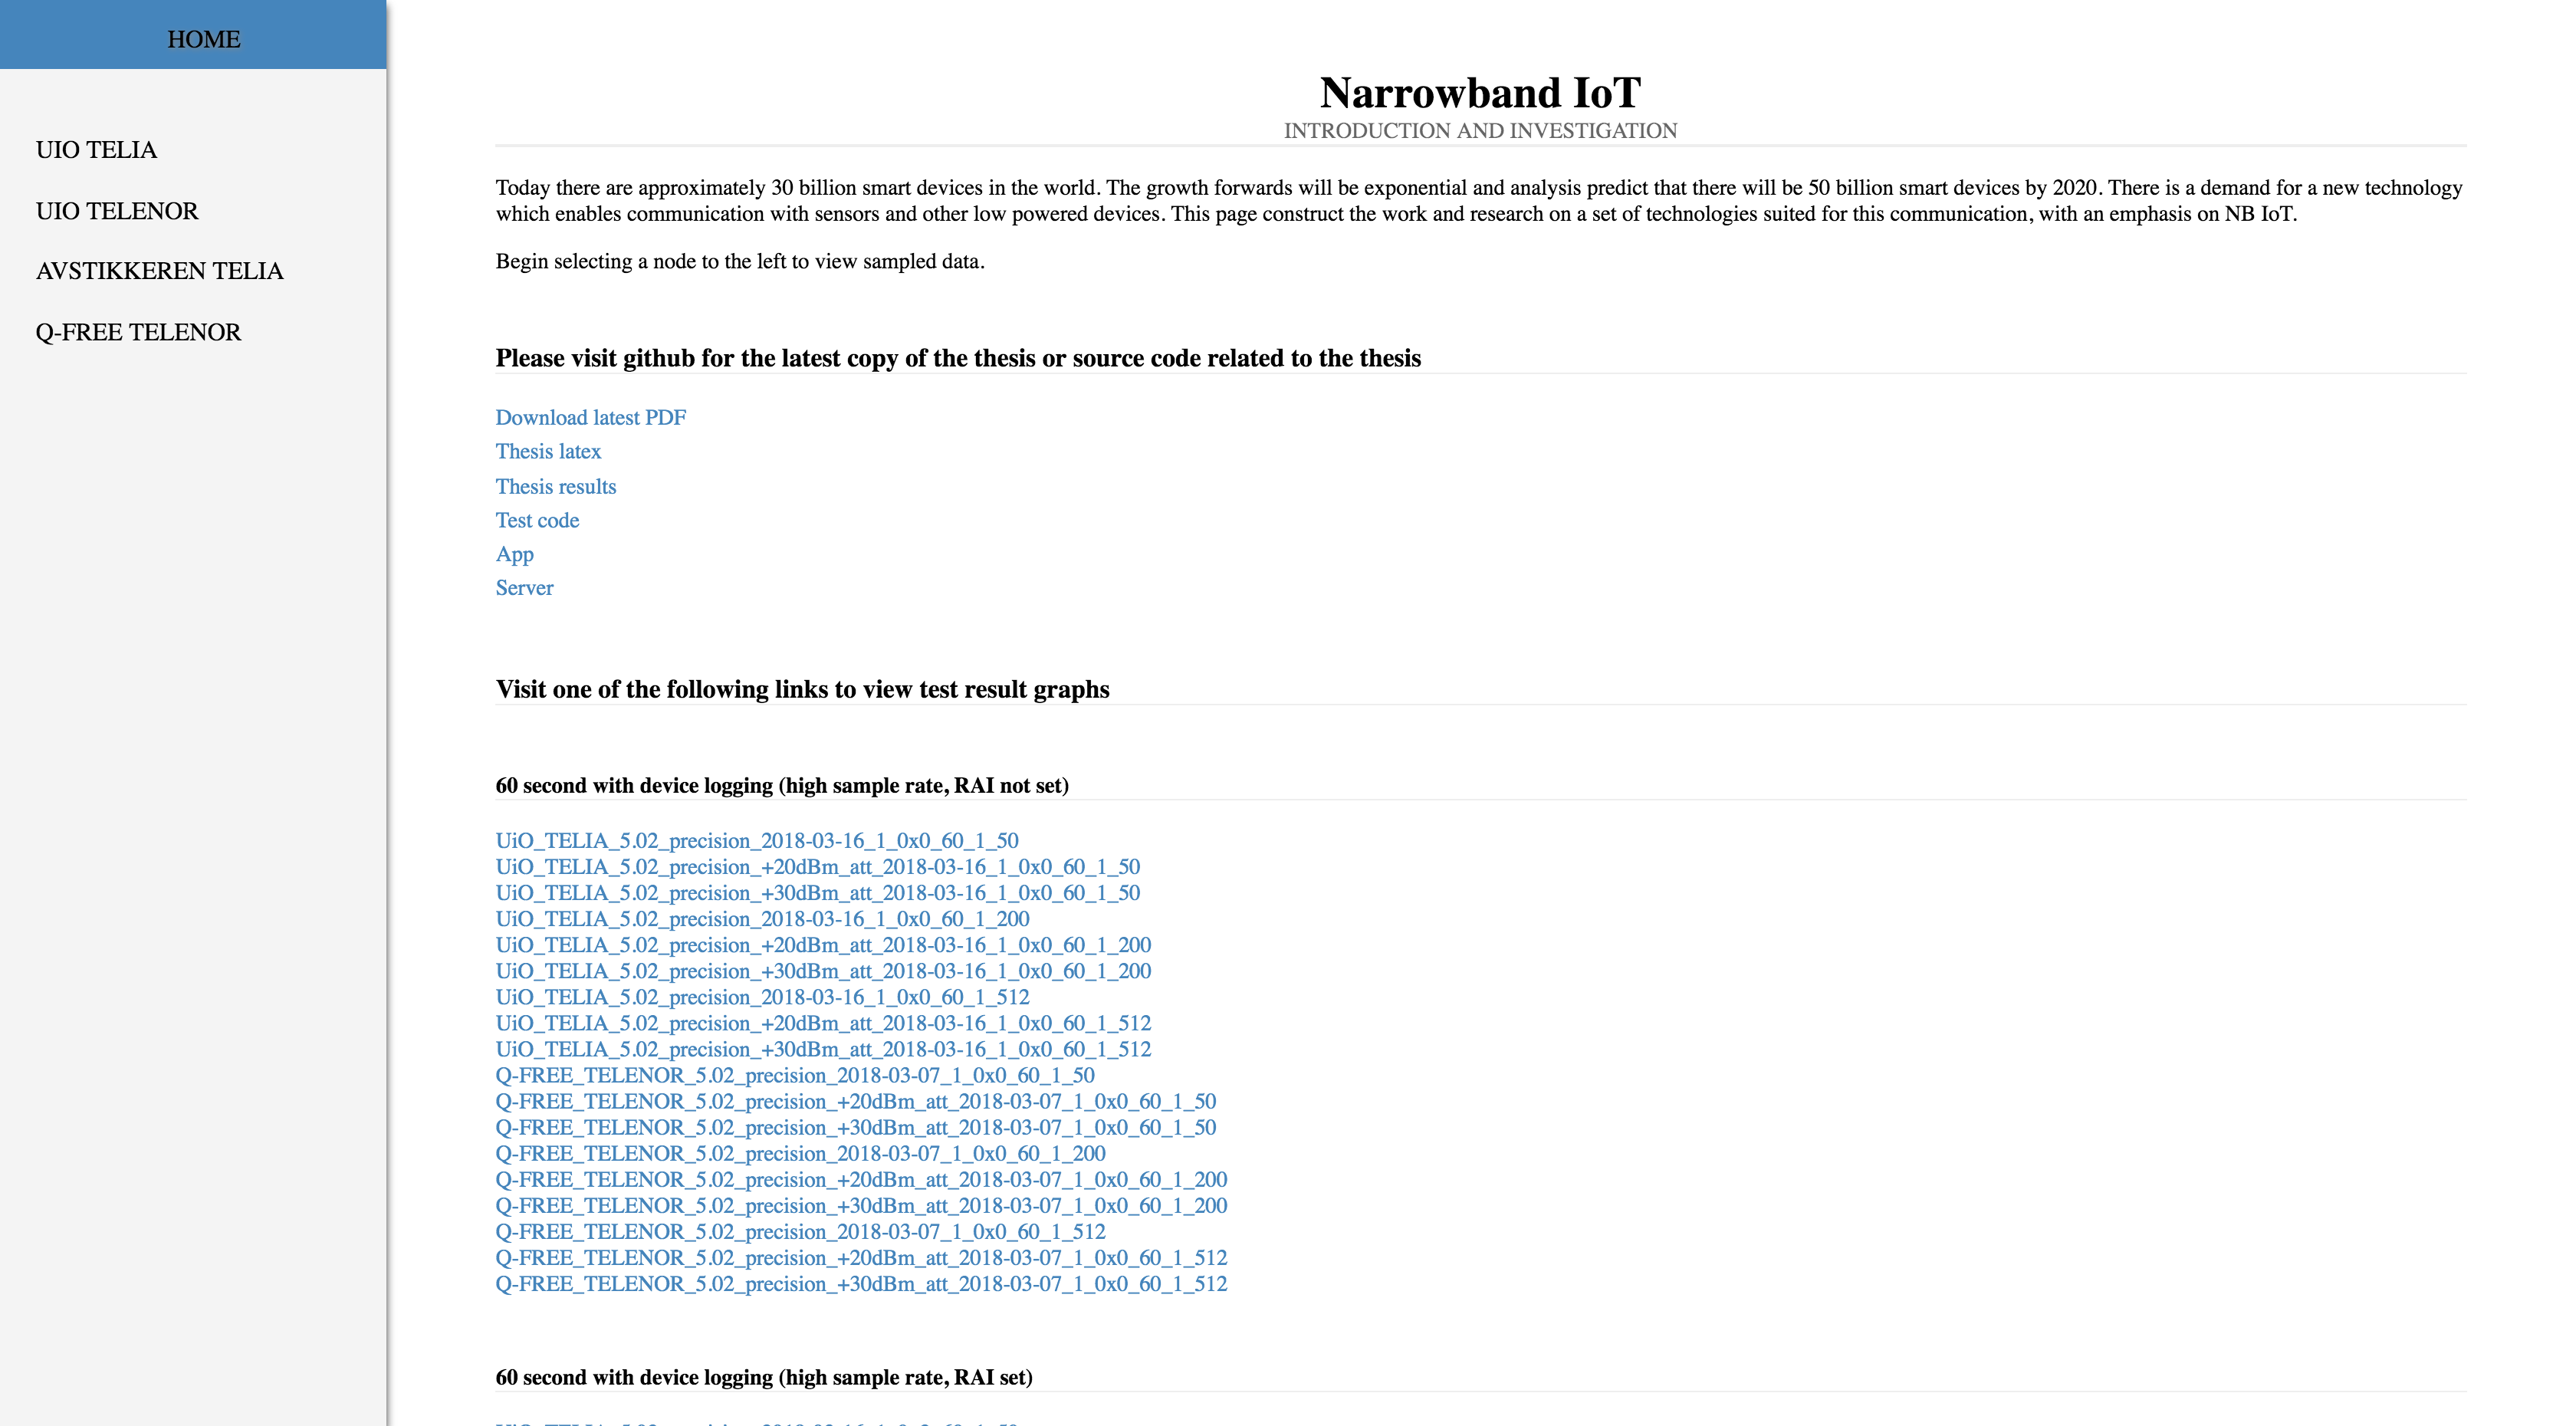
\includegraphics[width=\textwidth,height=9cm]{/Users/henninghakonsen/Dropbox/Masteroppgave/thesis/webapp/homepage.png}
  \caption{SensorApp homepage}
  \label{pic:homepage}
\end{figure}

\begin{figure}[H]
  \centering
  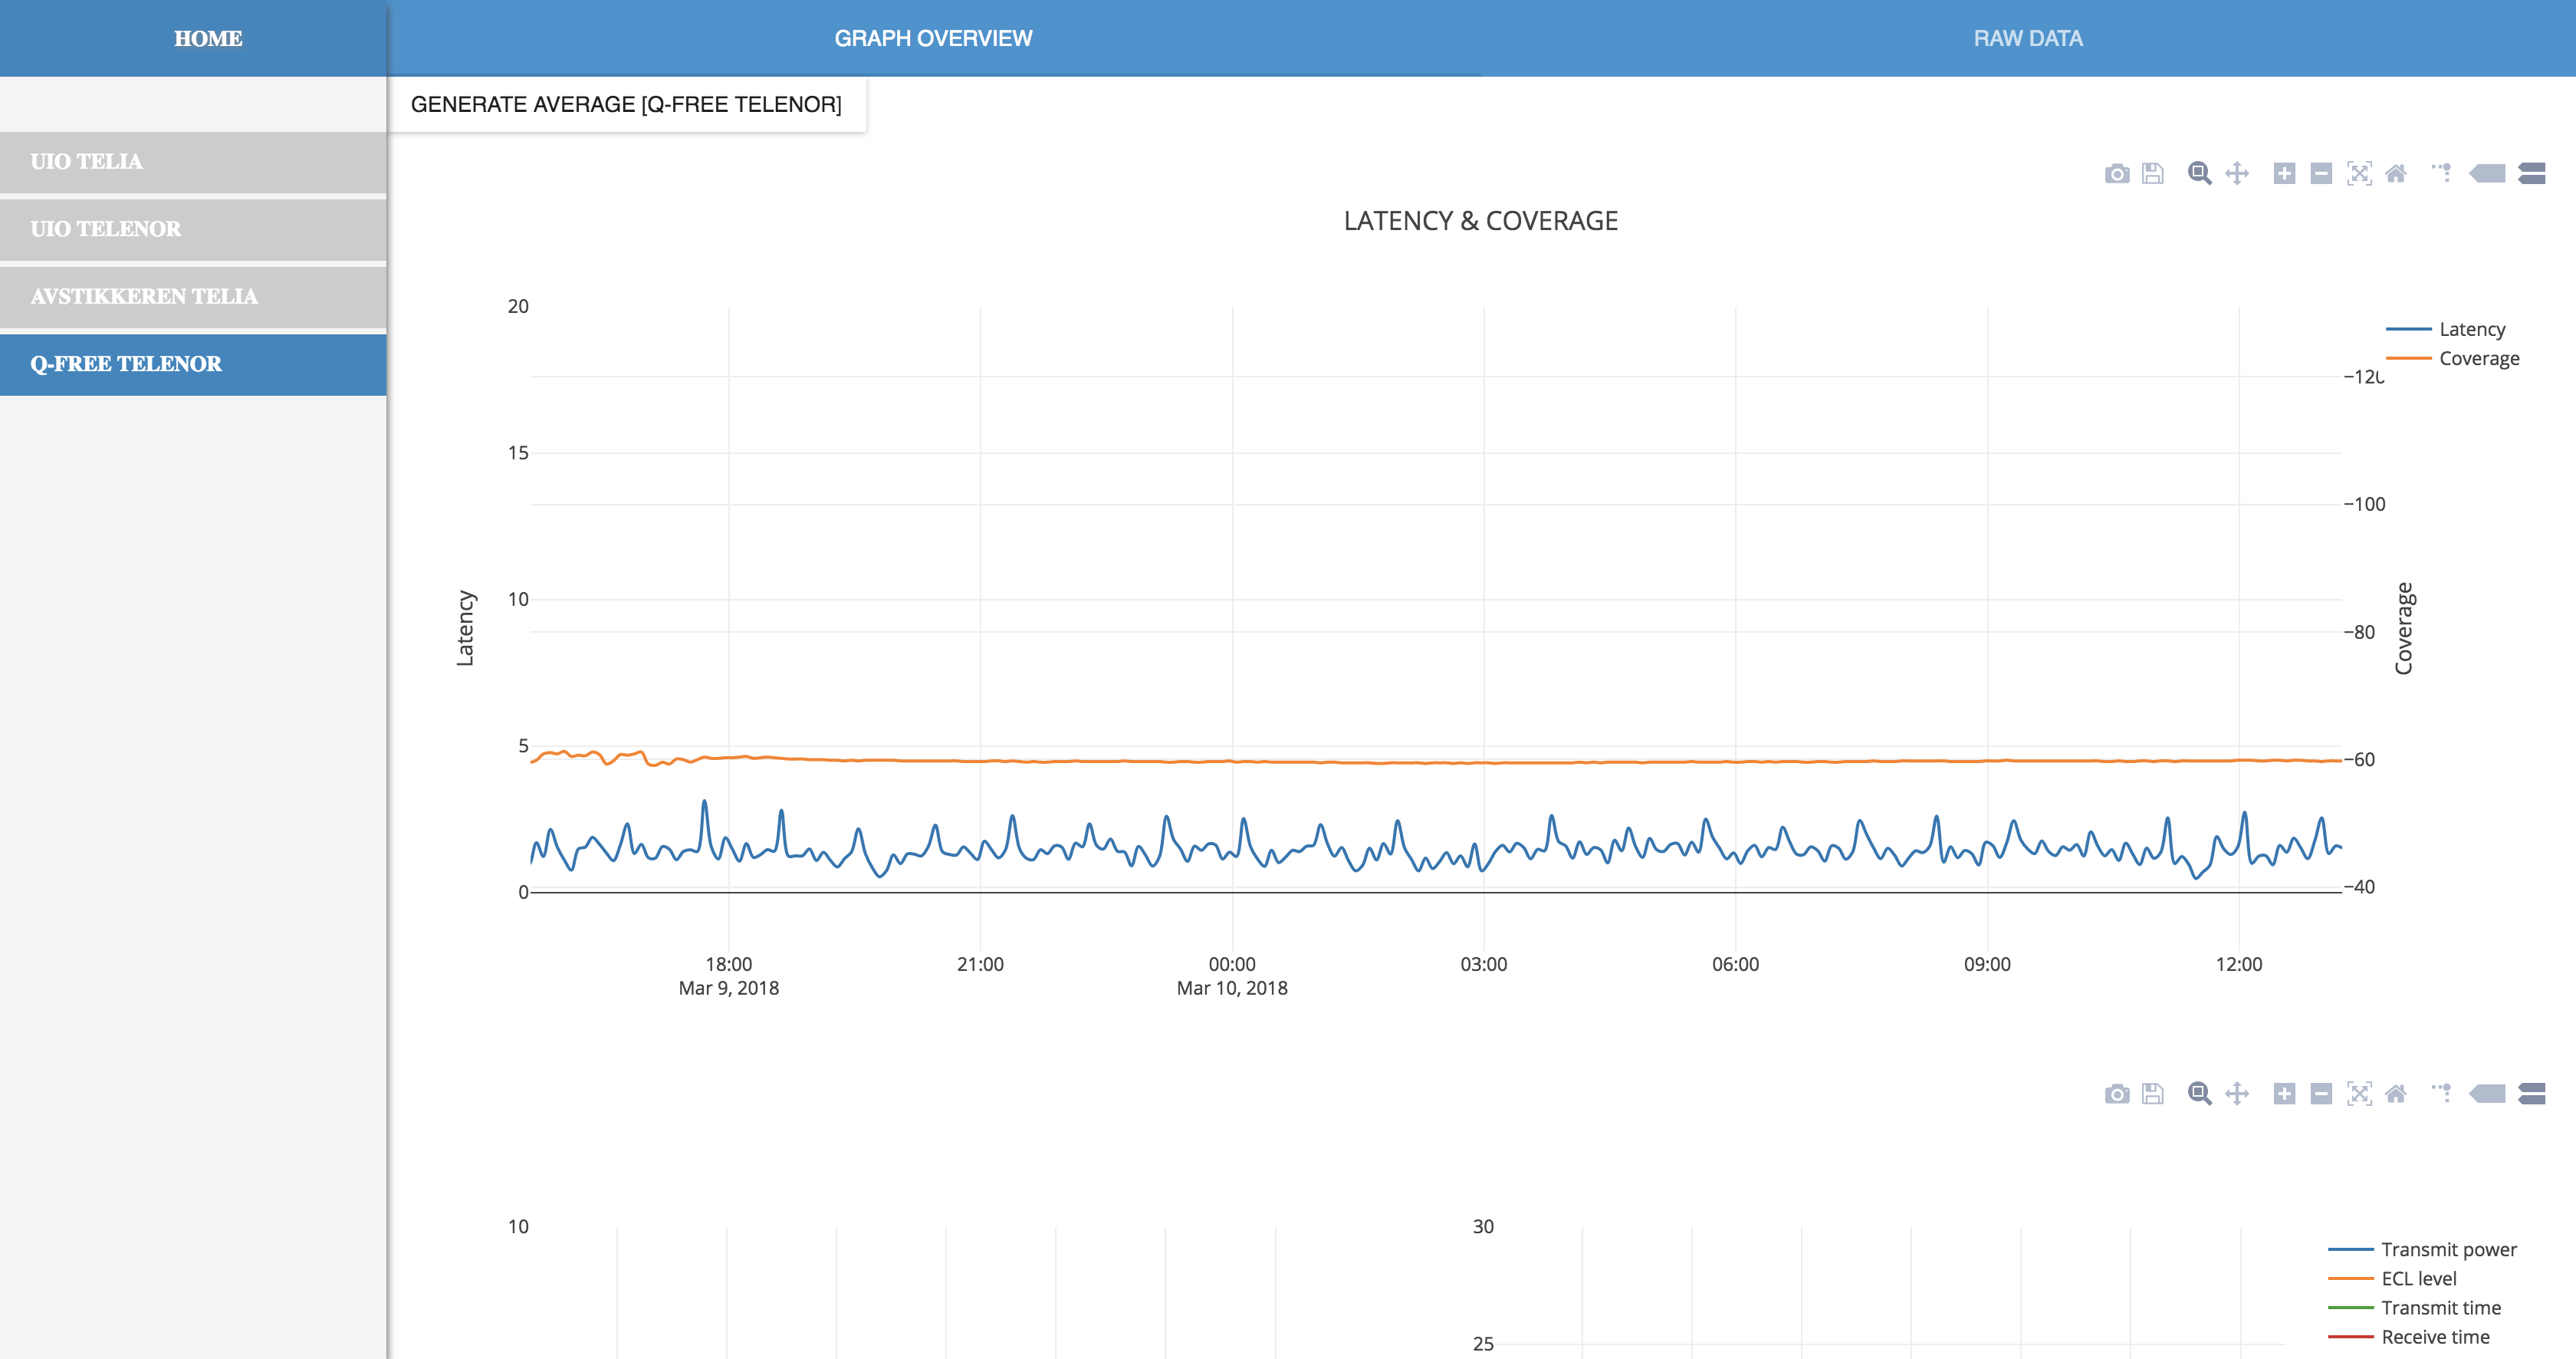
\includegraphics[width=\textwidth,height=9cm]{/Users/henninghakonsen/Dropbox/Masteroppgave/thesis/webapp/nodepage_1.png}
  \caption{SensorApp nodepage part 1}
  \label{pic:nodepage1}
\end{figure}

\begin{figure}[H]
  \centering
  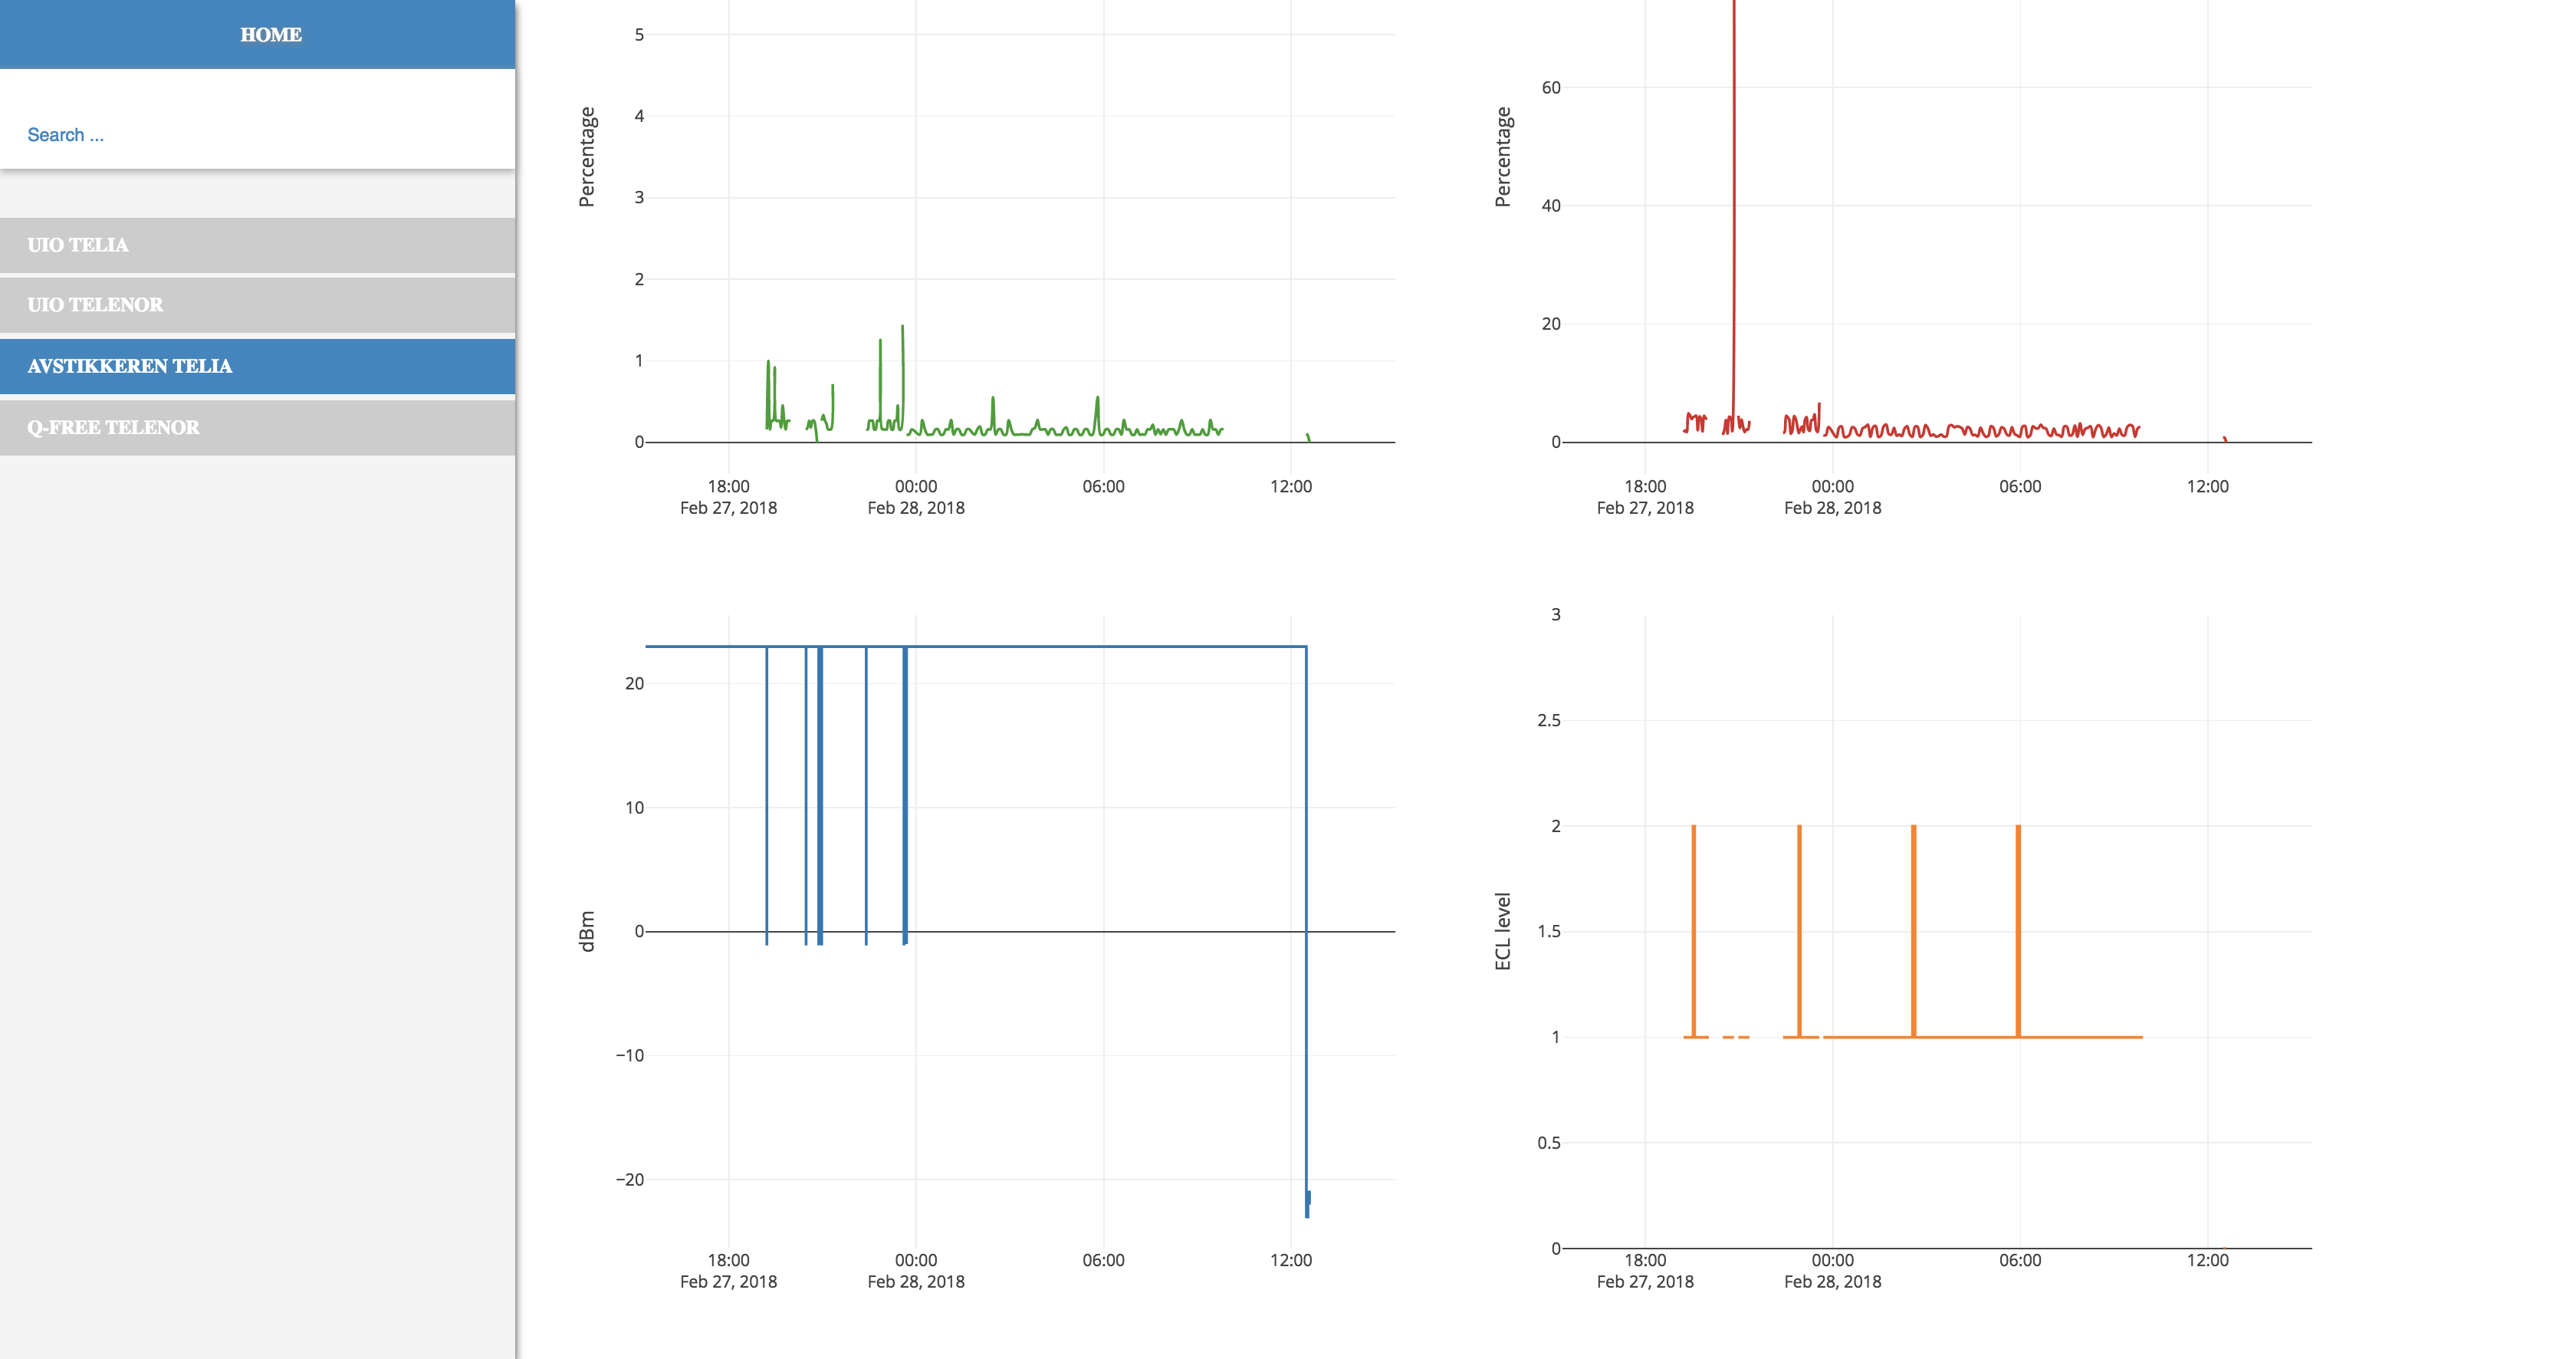
\includegraphics[width=\textwidth,height=9cm]{/Users/henninghakonsen/Dropbox/Masteroppgave/thesis/webapp/nodepage_2.png}
  \caption{SensorApp nodepage part 2}
  \label{pic:nodepage2}
\end{figure}

\subsection{Analysis} \label{ssection:analysis}
When selecting a node to explore you can explore the different graphs and we think this is a good way to display statistical data. The graphs data represents the output of the analysis on the server and we will try to describe what the graphs present and why we chose the different aspects of the behavior of the network.
In the following subsections we will introduce you to a set of features we will include in our analysis. Remember that the data is mostly produced by \textbf{AT+NUESTATS}, so read, \vref{section:deviations}, for any deviations.

\subsubsection{Coverage and Latency}
One of the main features of \acrshort{nb-iot} is coverage, hence we wanted to display coverage statistics over time. One interesting point of coverage is that it is closely related to the power usage of the device. The latency of \acrshort{nb-iot} is not a key feature, but the desired latency is under ten seconds according to the specifications\cite{datasheet:ubloxchip} and by displaying the latency in the same graph as coverage we can clearly see how the different coverage levels inflict latency in the network. The output of coverage and latency is directly from the output of \textbf{AT+NUESTATS}. To give a clearer understanding of coverage we have classified the coverage level into categories, see table \vref{table:coverage_cat}.

\begin{table}[H]
\centering
\resizebox{\textwidth}{!}{%
\begin{tabular}{|l|m{10cm}|}
  \hline
  \textbf{Coverage level(\acrshort{dbm})} & \textbf{Category} \\ \hline
  -40 to -60 & Excellent reception \\ \hline
  -60 to -80 & Good reception \\ \hline
  -80 to -100 & Quite good reception \\ \hline
  -100 to -110 & Bad reception \\ \hline
  -110 to -130 & Very bad reception \\ \hline
\end{tabular}%
}
\caption{Coverage categories}
\label{table:coverage_cat}
\end{table}

\subsubsection{Recieve and transmit time}
The output from \textbf{AT+NUESTATS} gives us a counter from receive and transmit time in milliseconds. We used the value between each entry to calculate how much time the receive and transmit time. The analysis produces a percentage which relates to how much time the device was in receive or transmit state in one interval. This is also closely related to the coverage of the device and also the \acrshort{ecl} level which indicates the number of retransmits per packet sent. The reason why we would like to monitor this data is because the device will mostly use power in these periods, so if the device is active for longer periods in either receive or transmit state we know that the expected lifetime is degraded. Most of the time the active percentage will be low due to usage of \acrfull{rai} and \acrshort{psm} mode, however if the transmit frequency is low the device will more frequently be in some kind of active state, hence the transmit and receive time will increase.

\subsubsection{\acrshort{ecl}}
The coverage mode is also closely related to the power usage of the device and an important factor we could monitor. You can clearly see that the power usage increases when the device enters \acrshort{ecl} mode 1 and 2 in the testing section, \vref{section:testing}. The output of \acrshort{ecl} level directly from the output of \textbf{AT+NUESTATS}.

\subsubsection{Transmit power} \label{paragraph:txpower}
The amount of power used for transmit is decided by software and is key to power usage. The output we get from \textbf{AT+NUESTATS} show us the latest transmit power level of the device. Sometimes the device will send a \acrfull{nack}, which is always sent with ${+23 \acrshort{dbm}}$ signal strength and is what \textbf{AT+NUESTATS} sometimes picks up as the latest transmit power level\cite{email:nack}. In the long term tests with graphs from the web app the logging of transmit power might not be correct related to what transmit power level the device actually used for transmitting the packet. However in the section on detailed tests, \vref{section:detailedtest}, we will log the status of the device up to ten times a second which will give a better understanding of what is happening with the transmit power level. In addition we will monitor the actual power usage with a multimeter, giving us more accurate test results.

\chapter{Testing} \label{section:testing}
In this part we will discuss the tests we performed. We will describe why and how we did each test and give you a detailed explanation of the results. In addition you will be presented an overview of the testing environments, devices and parameters that effected the tests. We have tried to include as many tests as possible and throughout this part we will analyze the results and at the end we will give a summary of the current \acrshort{nb-iot} situation.

The test phase began early January and was completed late March. The reason for the late test phase was due to a number of things. First of all, the hardware and software related to \acrshort{nb-iot} was not available on a stable platform until late 2017, and Telenor and Telia had limited \acrshort{nb-iot} enabled base stations. Even at the beginning of 2018 the devices we used were not production ready, but at that stage the error rate was very low. Because of the early adaption we encountered some interesting results, giving us an indication of the state of the technology. Given the hypothesis we needed to test the chip and the networks with good equipment and at several locations. In chapter, \vref{chapter:wherewhynhow}, we gave you an overview of the testing premises and the devices used.

In section, \vref{section:guidelines}, we will introduce a set of best practice guidelines to \acrshort{nb-iot} and we will include the results from the testing phase to so that you will see why the guidelines are as described.

\section{Short term tests} \label{section:detailedtest}
In this section we will investigate details about how the \acrshort{nb-iot} chip handles normal usage and edge cases where non default behavior is activated. What defines normal behavior? Normal operation of the \acrshort{ue} is when \acrshort{ecl} level is 0 and coverage better than -100dBm. When the \acrshort{ue} has bad reception it may retransmit packets and operation like this over longer periods is not sustainable. With normal operation we also expect the \acrshort{ue} to transmit packets with \acrshort{rai} set and \acrshort{psm} activated. According to the specifications the device will enter deep sleep mode trailing a each transmit.

We define short term tests as a logging sequence over a short period with frequent data points. The duration of the tests are under ten minutes and the sample rate is high, over 300 samples per second for some tests. These tests will show you how the device performs on a detailed level and will give a good understanding og the transmit process. The reason for including these tests are related to the actual power usage over a short period. By defining power usage statistics for different kinds of transmit we will be able to normalize the data and give an estimation of expected lifetime based on our tests. The detailed tests also will show us if the network providers follow the specifications. It is very interesting to follow \acrshort{psm}, connection status, coverage and power usage over a short period and see how the device handles different scenarios.

We have sectioned the results into categories and we will refer to a set of graphs located after the section. In this way you will be presented with one problem at a time while pointing to the same graphs. To explore the full potential of the graphs you may also visit the thesis web page\cite{url:thesispage}, which is supplied in the caption of each figure.

\subsection{General} \label{ssection:generaltest}
Most of our short term tests were performed with an emphasis on power usage, rather than coverage and latency. It is however clear that high power usage is a side effect of bad coverage. All our tests show that better reception gives lower latency and power usage. However, in the case of our test with Telia at Q-Free we saw that even with good reception we got poor and weird results. Looking at figure, \vref{figure:2x150_QFREE_TELIA_SHORT}, we see that the device is having trouble entering \acrshort{psm} mode even though the expired 120 seconds has elapsed. We saw that the device does not leave RRC connected mode, hence the power usage will increase. The reception of the device at this location was good and the \acrshort{snr} values was much like Telenor's at the same location. In this test we did not use the \acrshort{rai} so the expected behavior would be transmit at the beginning of the program, following a period of 20 seconds in RRC mode. After this the device should enter \acrshort{edrx} mode, only receiving data on a set interval, normally 2-25 seconds, with a number of receive transactions within each \acrshort{edrx} period. After this period the device should enter \acrshort{psm} mode if it is enabled by software. However, in this test it looks like the device is performing \acrshort{drx} and polling for data from the network very frequent. Looking at the network connection graph you see that the device does not leave this state until it suddenly indicates loss of connection and rapidly reestablishing connection and transmits the last packet. Directly before the last transmit we see a short period of frequent receive transactions. This might be related to the loss of connection, presuming that the \acrshort{ecl} level is delayed until connection is restored. An alternative is that due to the bad configuration the time of the paging window negotiation is longer than expected, resulting in a period of constantly trying to receive data from the network. If we continue looking at the time of the last transmit we see something interesting with the transmit power. After renegotiating the connection towards the network the transmit power is adjusted from around ${+6 \acrshort{dbm}}$ to ${+23 \acrshort{dbm}}$ even though the signal power is kept at the same level. At this location most of the tests showed some kind of flaw in the network, either related to packets being dropped, long transmit times or trouble following the normal transmit procedure. It would be interesting to investigate what happened of the network side of this setup. The network becomes a black box and when the network performs out of the ordinary it is hard to debug.

\begin{figure}[H]
  \centering
  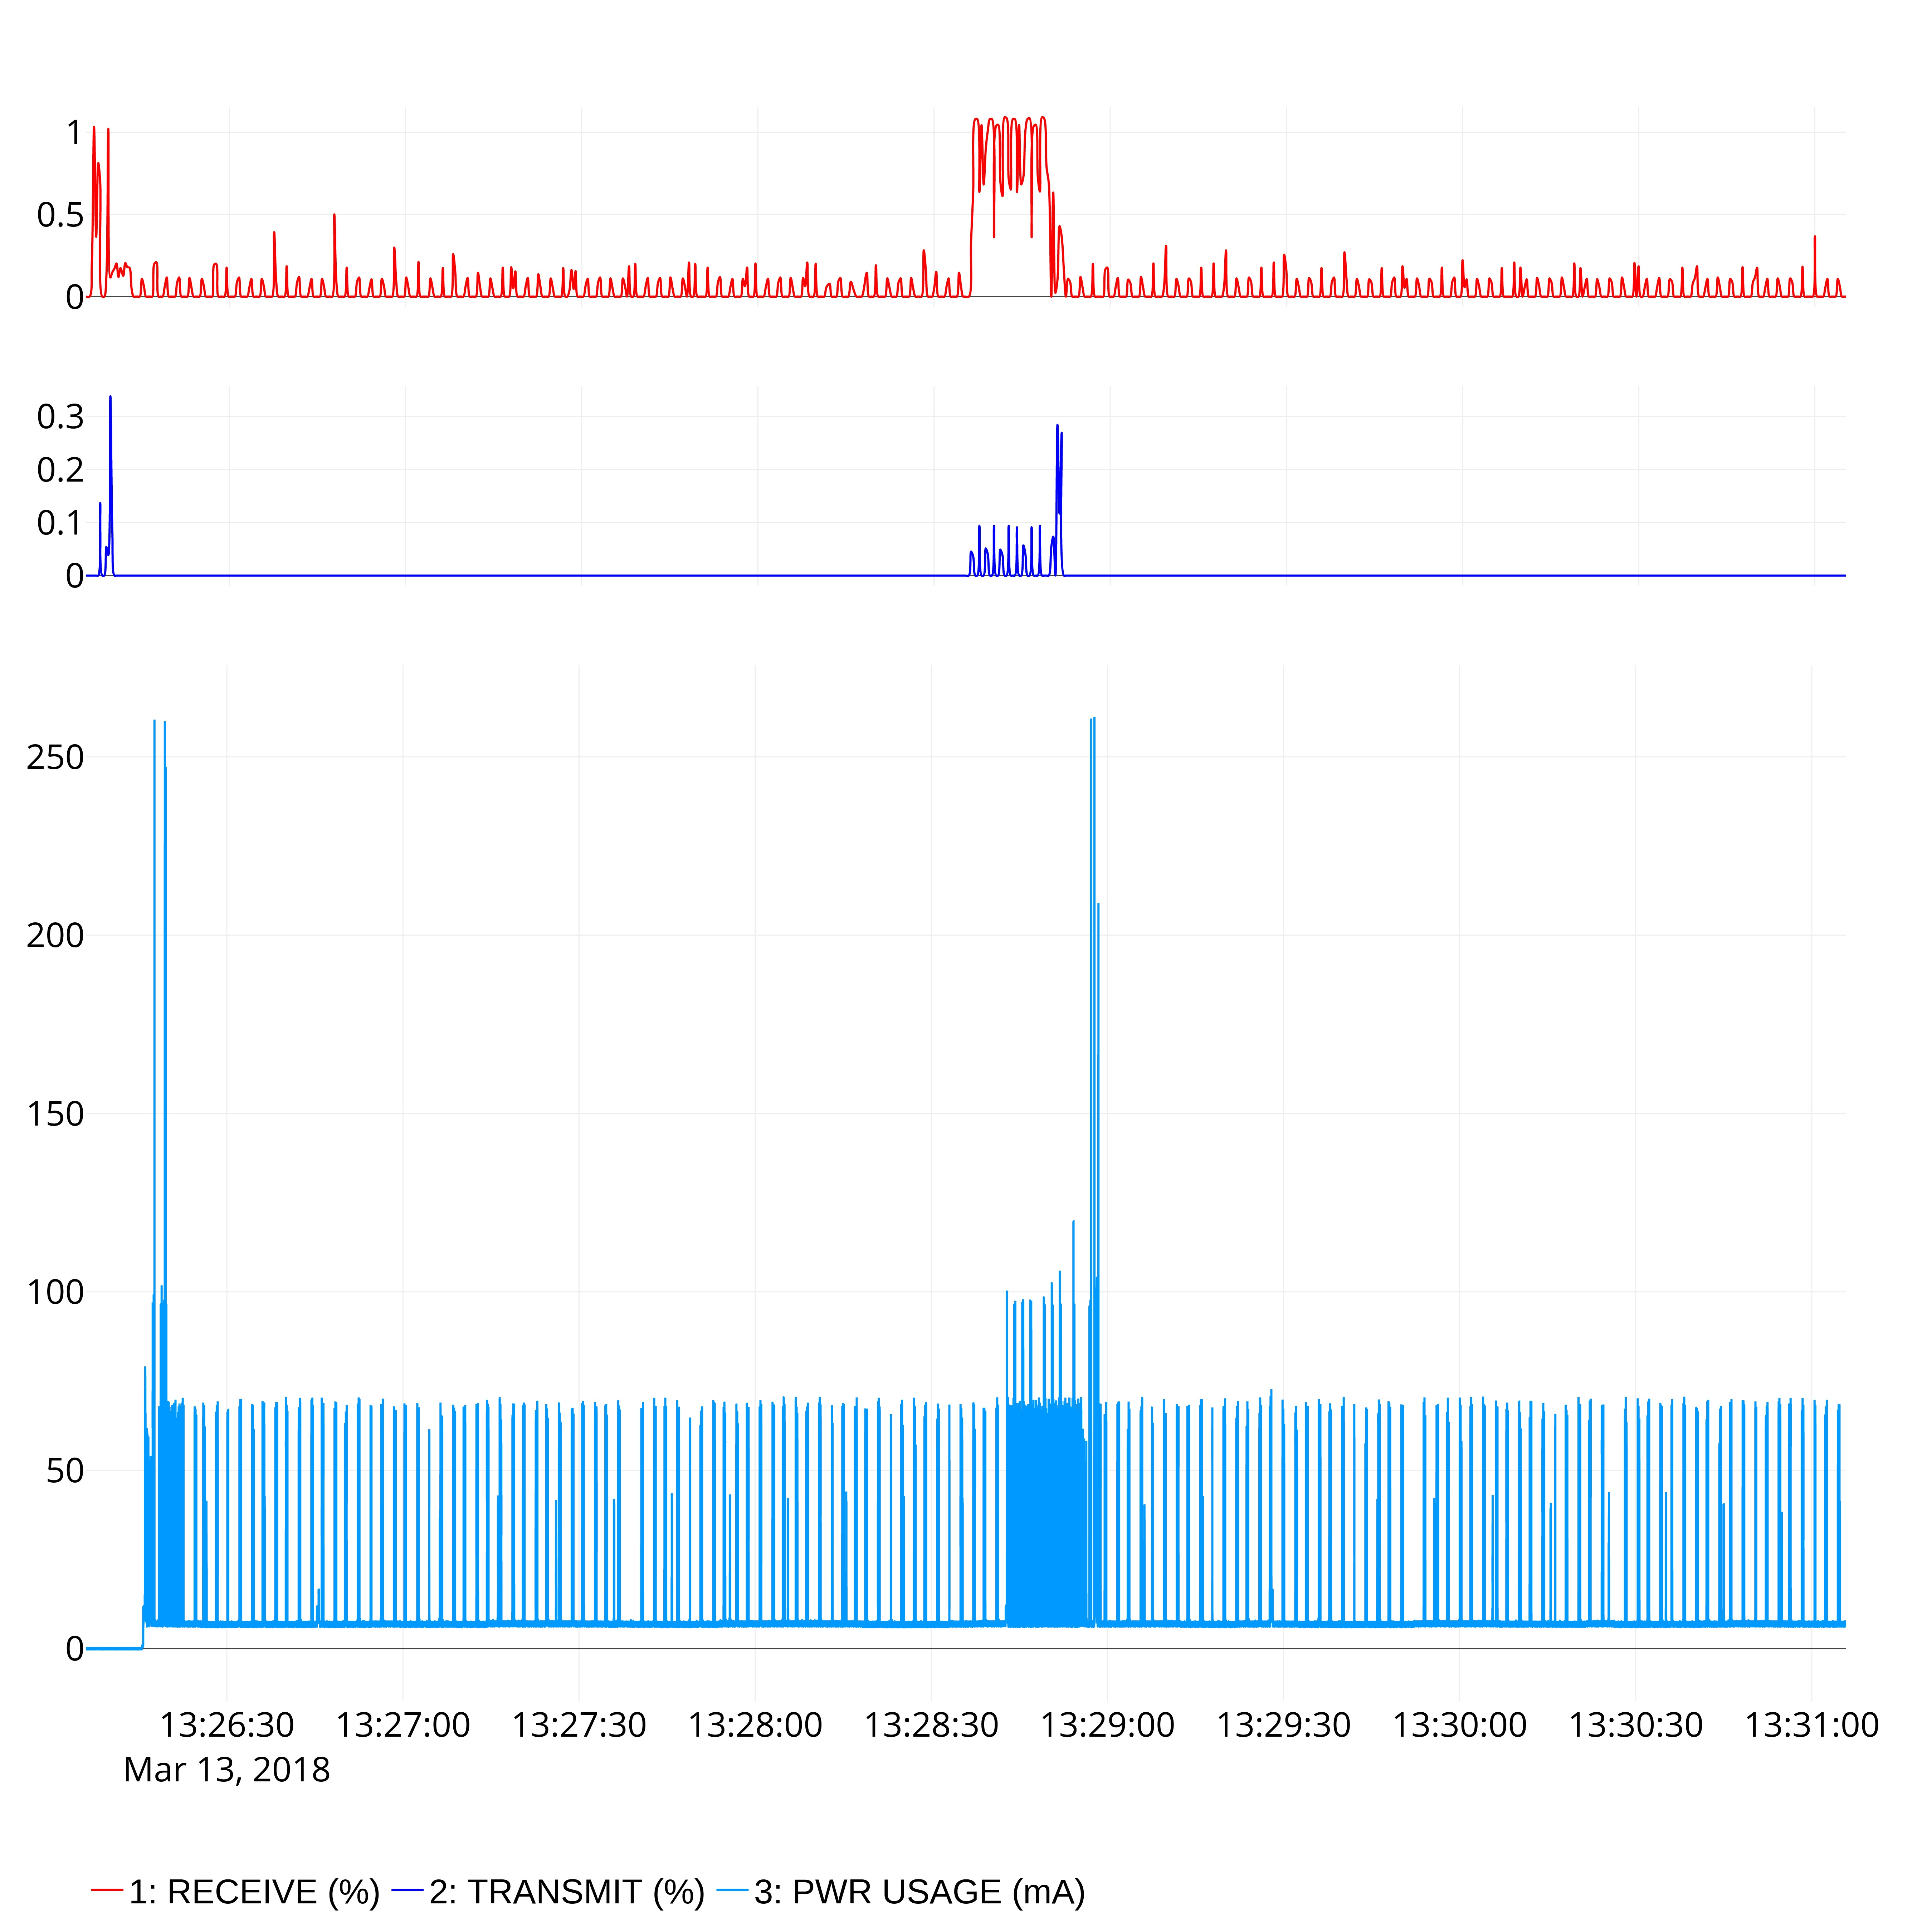
\includegraphics[width=\textwidth, height=0.4\textheight]{/Users/henninghakonsen/Dropbox/Masteroppgave/thesis/latex/images/short_Q-FREE_TELIA_5_02_precision_2018-03-13_1_0x0_150_2_100.jpeg}
  \caption{Weird behavior, Telia. See figure, \vref{figure:2x150_QFREE_TELIA}, or visit, \href{http://158.39.77.97:9000/\#/results/Q-FREE\_TELIA\_5.02\_precision\_2018-03-13\_1\_0x0\_150\_2\_100}{webapp} \cite{online:result0}, for more details.}
  \label{figure:2x150_QFREE_TELIA_SHORT}
\end{figure}

With this in mind we will show a similar presentation of a proper transmit procedure, form Telia and Telenor, followed by a walkthrough of the same process only without device logging. Looking at figure, \vref{figure:2x150_UIO_TELIA_SHORT} and \vref{figure:2x150_QFREE_TELENOR_SHORT}, the process is totally different and is looking more like a graph representation of the specifications. Looking first at the graphs from UiO with Telia we see two transmit periods of around 20 seconds. Following a period of \acrshort{edrx} and then \acrshort{psm}. We were not using the \acrshort{rai} in this test either, hence the RRC period of 20 seconds. Notice that the device is not pulling for data all the time within the RRC period. It usually receives a lot of data when initiating the uplink transmit, but after the transmit it only pulls for data around 20\% of the time, hence reducing the power usage. When asking Telia about this they state that this is most likely related to \acrshort{drx} process which kicks in because there are not any data to receive\cite{email:telia}. However, we did not manage to figure out why the device performed this way when connected to Telia and not Telenor.
It is also worth noting that when the device is not in RRC mode the statistics from \textbf{NUESTATS} become stale. This is an indication of deep sleep mode, and in \acrshort{edrx} the device should sleep between each \acrshort{edrx} period. We can see that after two \acrshort{edrx} periods the device enters \acrshort{psm} with permission from the network.

Moving focus over to Telenor we can also see some distinct differences from Telia's transmit process. The first thing we noticed was that Telenor is pulling for data close to 100\% of the time spent in RRC mode. This results in an increase of 5 in terms of pure power usage compared to Telia's solution. We can see that the current at this stage is comparable, at around ${60-70 \acrshort{ma}}$, a little higher than Ublox specification on page 16\cite{datasheet:ubloxchip}. If you look at the graphs from the website you are able to zoom in on these periods, revealing that Telia's RRC period is mostly using ${6-7 \acrshort{ma}}$, only flickering up to ${60-70 \acrshort{dbm}}$ when actually receiving. Telenor's RRC period however is mostly at ${50-60 \acrshort{ma}}$. It is clear that there are different configurations in the networks resulting in actual receive time. A part from this, the graphs have the same characteristics. One thing worth noticing is the adjusted transmit power because of the excellent reception at Q-Free. The device has ${-55 \acrshort{dbm}}$ signal power resulting in ${-24 \acrshort{dbm}}$ transmit power, almost minimum. This is clearly reflected in the power usage graph where Telenor only uses at most ${70 \acrshort{ma}}$ when transmitting, while Telia at ${+9 \acrshort{dbm}}$ transmit power is reaching ${110 \acrshort{ma}}$ at transmit time. Notice that this is close to what Ublox self is stating in their specifications. It is however lower than our calculations and we will discuss this in section about deviations, \vref{section:deviations}.

\begin{figure}[H]
  \centering
  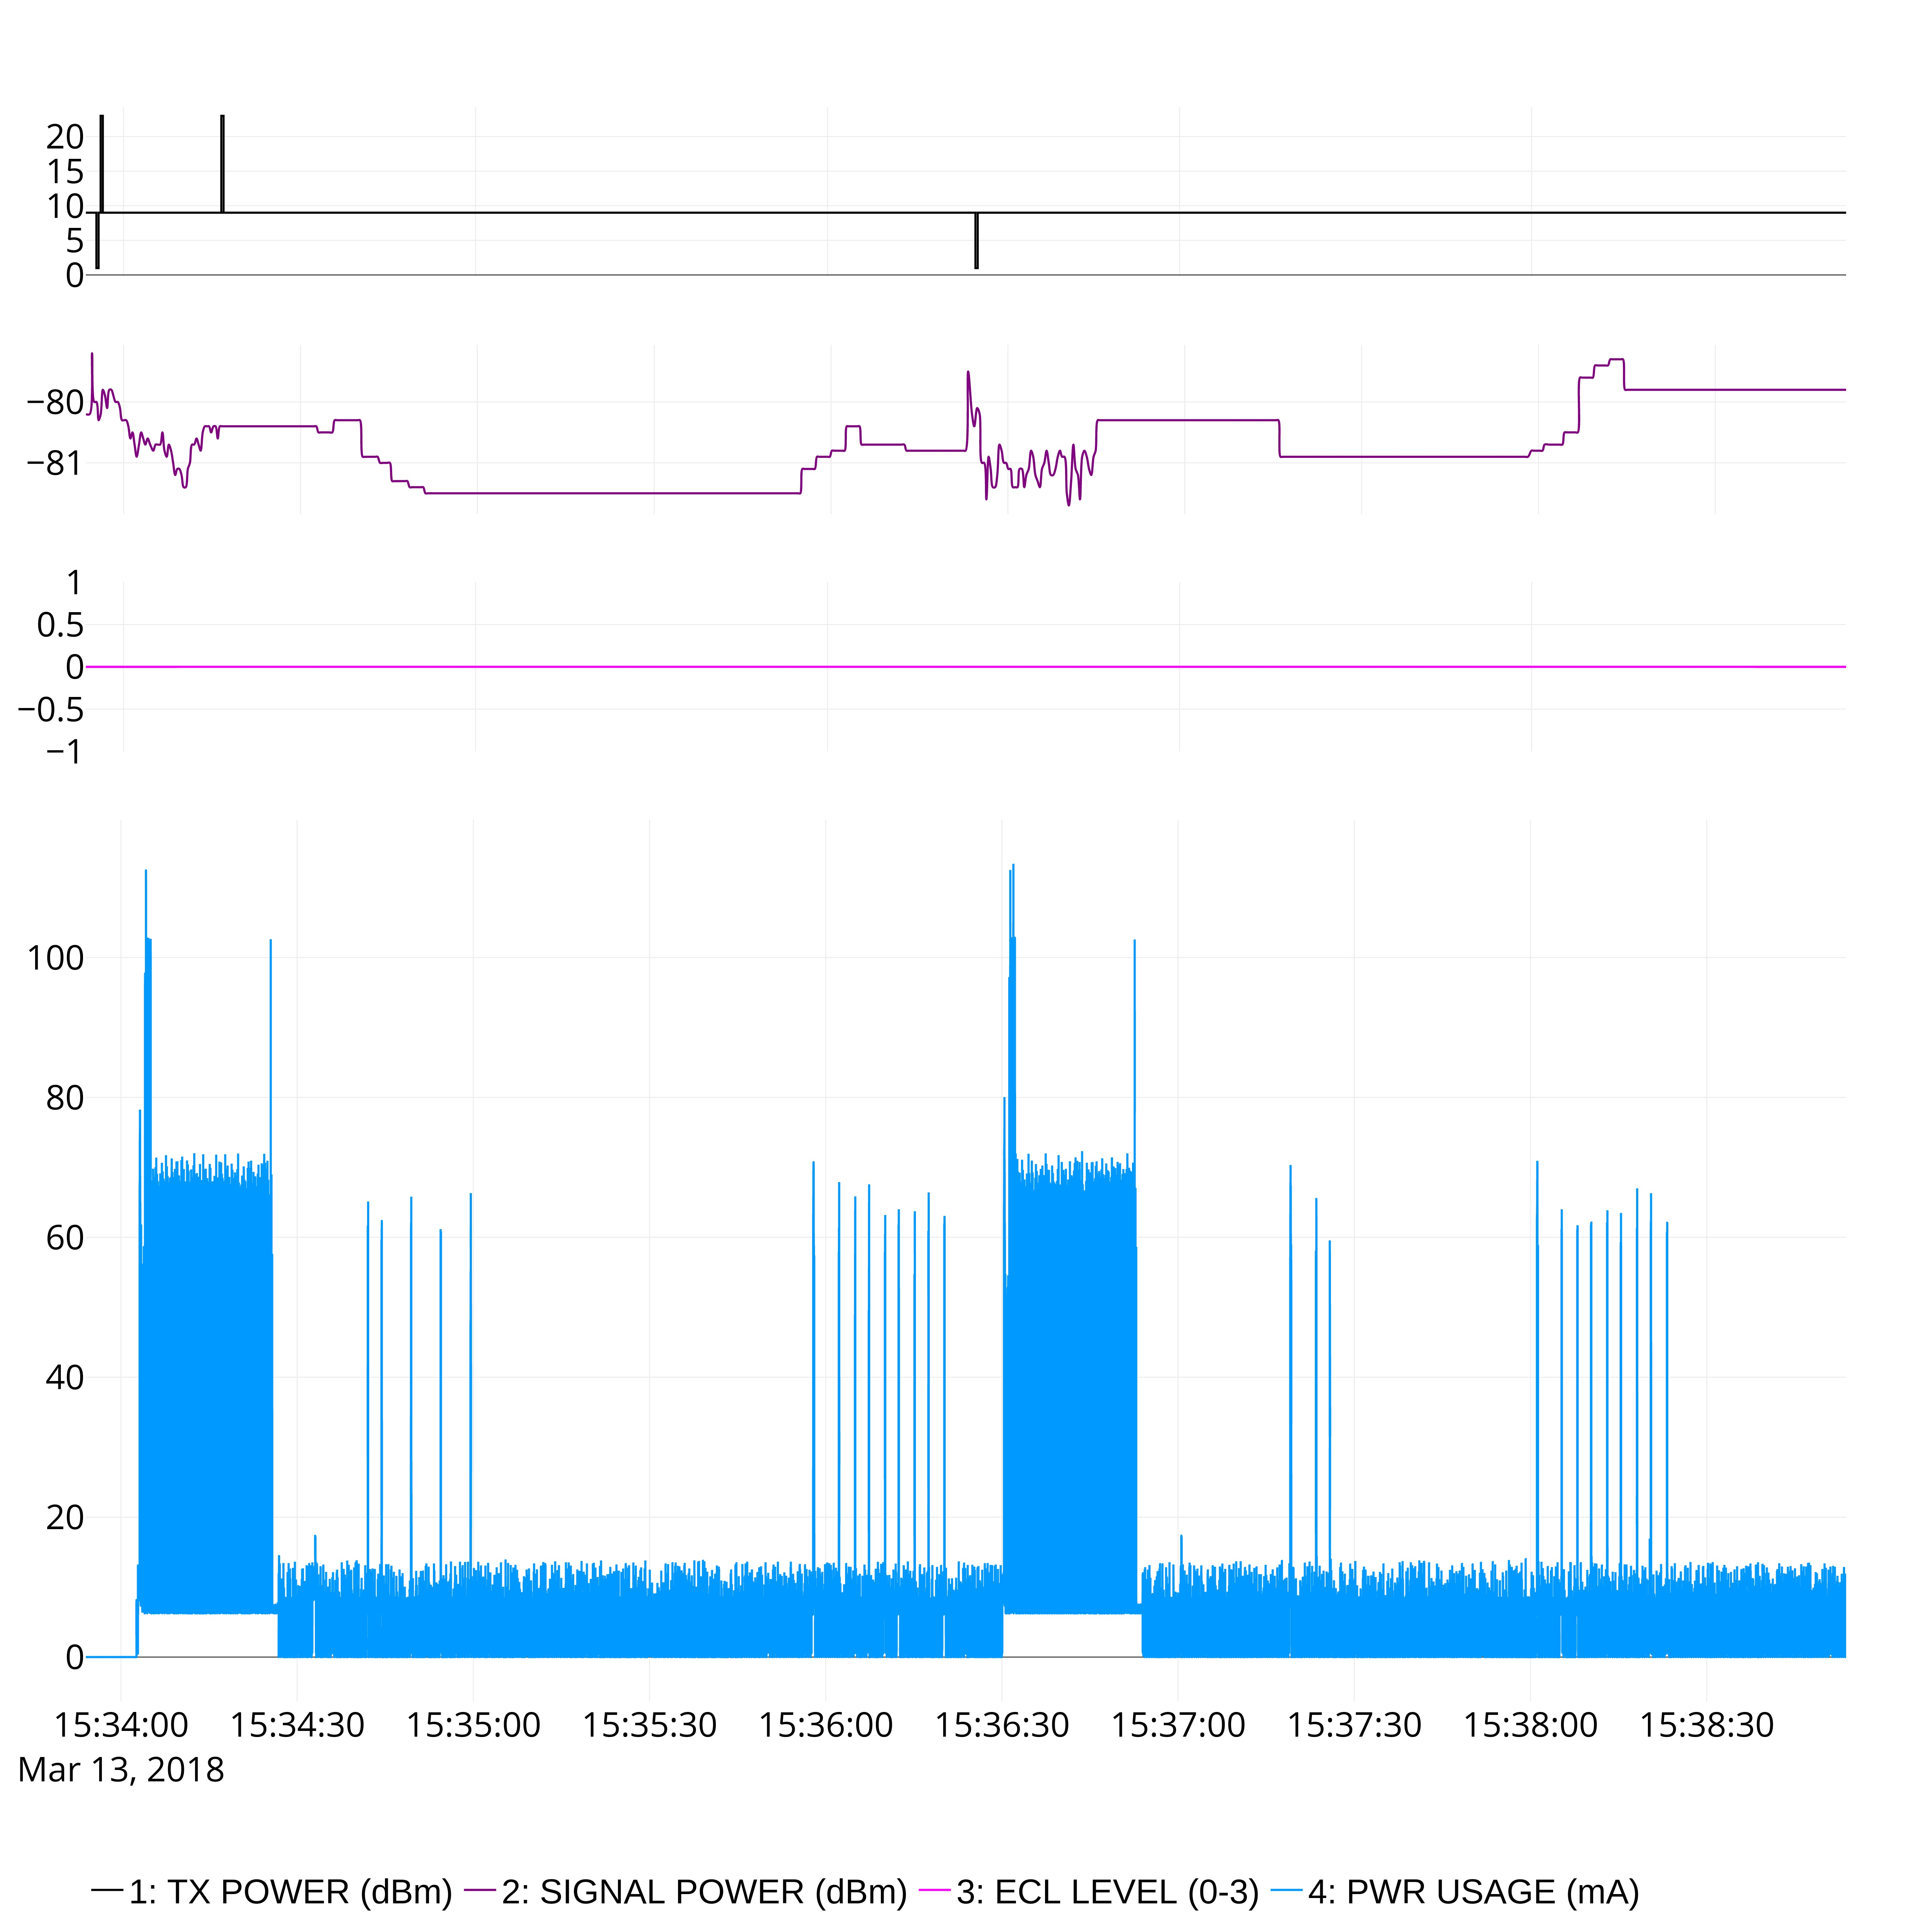
\includegraphics[width=\textwidth, height=0.4\textheight]{/Users/henninghakonsen/Dropbox/Masteroppgave/thesis/latex/images/short_UiO_TELIA_5_02_precision_2018-03-13_1_0x0_150_2_100.jpeg}
  \caption{Normal behavior, 2 x 150 UiO, Telia. See figure, \vref{figure:2x150_UIO_TELIA}, or visit, \href{http://158.39.77.97:9000/\#/results/Q-FREE\_TELENOR\_2018-02-28\_1\_0x0\_150\_2\_100}{webapp} \cite{online:result1}, for more details.}
  \label{figure:2x150_UIO_TELIA_SHORT}
\end{figure}

\begin{figure}[H]
  \centering
  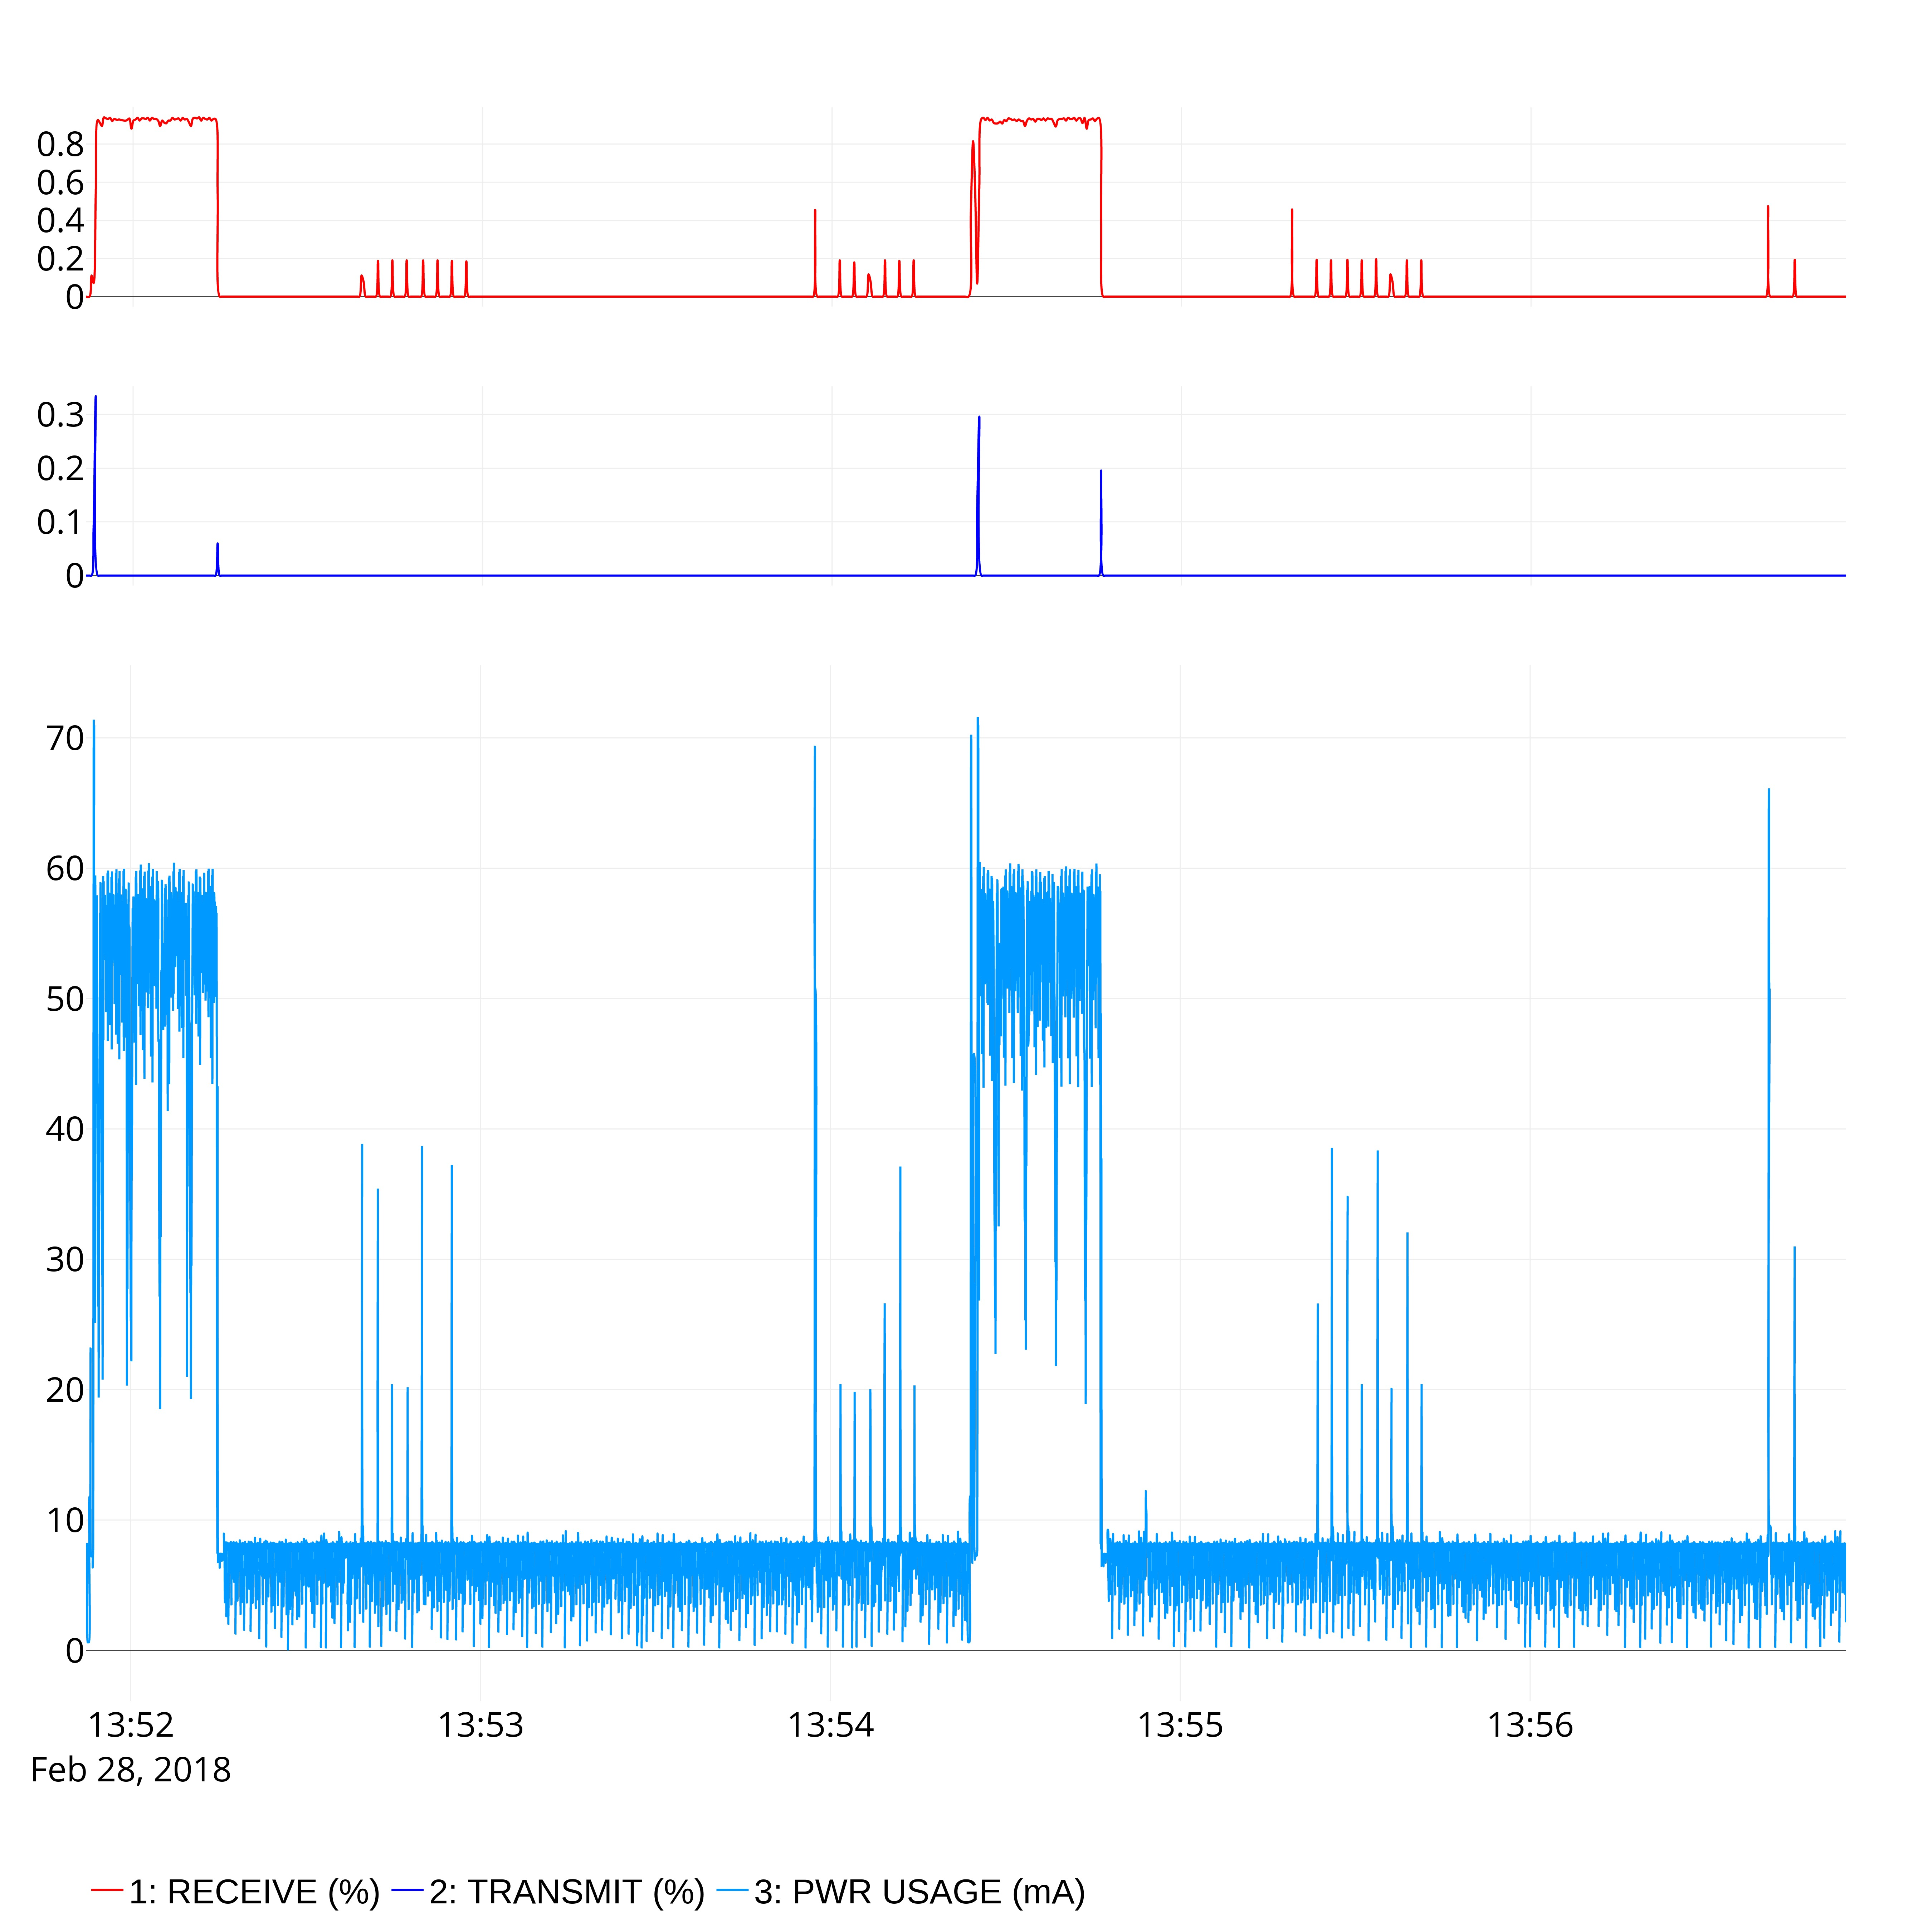
\includegraphics[width=\textwidth, height=0.4\textheight]{/Users/henninghakonsen/Dropbox/Masteroppgave/thesis/latex/images/short_Q-FREE_TELENOR_2018-02-28_1_0x0_150_2_100.jpeg}
  \caption{Normal behavior, 2 x 150 Q-FREE, Telenor. See figure, \vref{figure:2x150_QFREE_TELENOR}, or visit, \href{http://158.39.77.97:9000/\#/results/Q-FREE\_TELENOR\_5.02\_2018-03-07\_0\_0x0\_40\_1\_200}{webapp} \cite{online:result2}, for more details.}
  \label{figure:2x150_QFREE_TELENOR_SHORT}
\end{figure}

\subsection{Transmit power spike}
Disregarding coverage level, one thing we noticed while doing most of the tests was that there was often a spike of power usage up to ${230 \acrshort{ma}}$. We have not included all graphs in this paper, but visiting \url{henninghaakonsen.me} you can view results tagged with 60x1 for Telenor for example. You will see this spike in many of the graphs and it is an interesting fund we would probably not find without the precision multimeter. The context of the occurrences is when the device is in RRC mode, hence in active communication with the network - either \acrshort{ul} or \acrshort{dl}. As explained in paragraph, \vref{paragraph:txpower}, a \acrshort{nack} is sent with ${+23 \acrshort{dbm}}$ transmit power, hence we have reason to believe that this is what is happening at these spikes. This behavior is not mentioned in the specification, and at the moment of the tests there were instances of this behavior than without. We also saw this behavior with Telia's network, so it is likely that this is normal procedure in a transmit process. It is however somewhat strange that this happens with transmits when the signal power is excellent, we would presume that this practice would only be in case of bad reception and signaling faults.

\subsection{Loss of connection prior to transmit} \label{ssection:ecl_255}
We performed some tests on Telenor's network at Q-Free with interval at 40 seconds with and without \acrshort{rai}. At many of these transmits we saw that the device indicated network disconnection directly before transmitting the packet. This results in a period with \acrshort{ecl} level at 255 and higher power usage for a short period where the device reconnected to the network. We have included two figures in section, \vref{figure:1x40_QFREE_TELENOR_0LOG_SHORT} and \vref{figure:1x40_QFREE_TELENOR_1LOG_SHORT}, representing this behavior. In both these tests, there is a period of reconnection to the network, followed by the actual transmit process. This pre-procedure of reconnecting to the network operates at a current of ${45-55 \acrshort{ma}}$ and is comparable to a RRC period or transmitting with very good reception.
In these tests the reconnection time has been rather low, but you will see in the long term tests, \vref{section:longtermtest}, that this is not always the case. This behavior is regardless of the \acrshort{rai} flag, hence the power usage is a lot higher compared to the actual transmit process when using the \acrshort{rai} flag. This is a root problem users and developers would have a hard time finding, and could cause battery lifetime issues. We estimate that this 5 second period uses ${(50 \acrshort{ma} / 60 / 60 ) * 5S = 0.069\acrshort{mwh}}$, which is actually twice as much as a normal transmit(see \href{http://158.39.77.97:9000/\#/results/Q-FREE_TELENOR_SHORT_TEST_2018-02-28_0_0x2_5_1_100}{webapp} \cite{online:result11}) with \acrshort{rai} set and excellent signal power.

\begin{figure}[H]
  \centering
  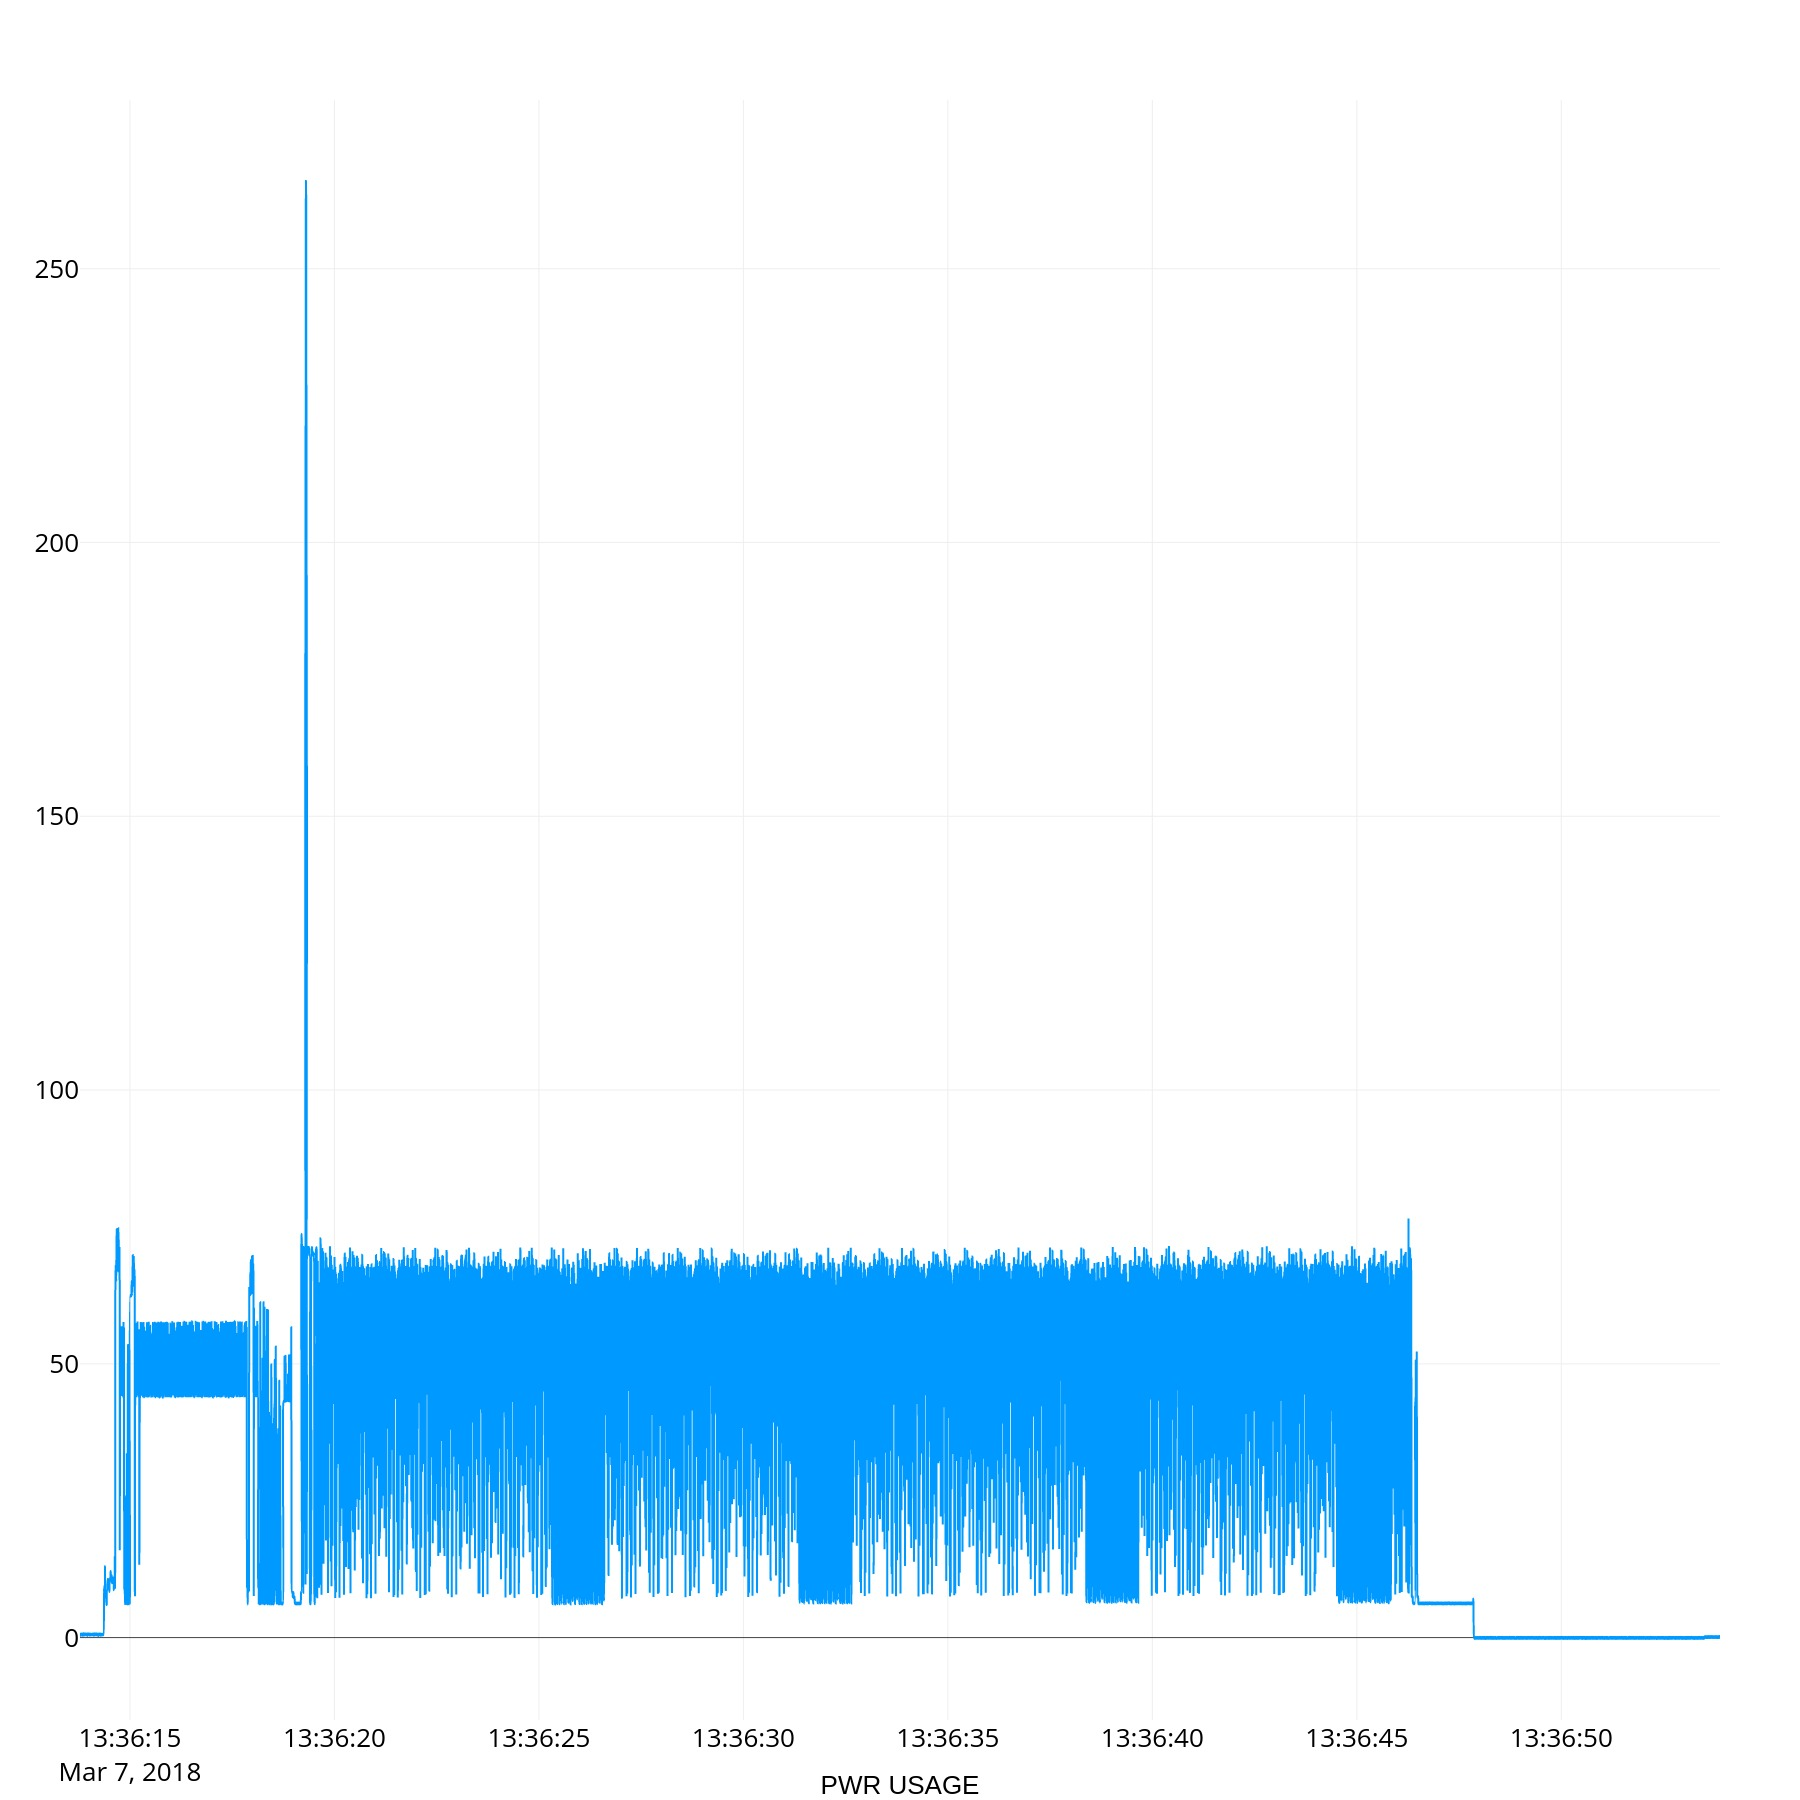
\includegraphics[width=0.9\textwidth, height=0.4\textheight]{/Users/henninghakonsen/Dropbox/Masteroppgave/thesis/latex/images/short_Q-FREE_TELENOR_5_02_2018-03-07_0_0x0_40_1_200.jpeg}
  \caption{1 x 40 Q-FREE, Telenor - no device logging. Visit, \href{http://158.39.77.97:9000/\#/results/Q-FREE_TELENOR\_5.02\_2018-03-07\_0\_0x0\_40\_1\_200}{webapp} \cite{online:result3}, for more details.}
  \label{figure:1x40_QFREE_TELENOR_0LOG_SHORT}
\end{figure}

\begin{figure}[H]
  \centering
  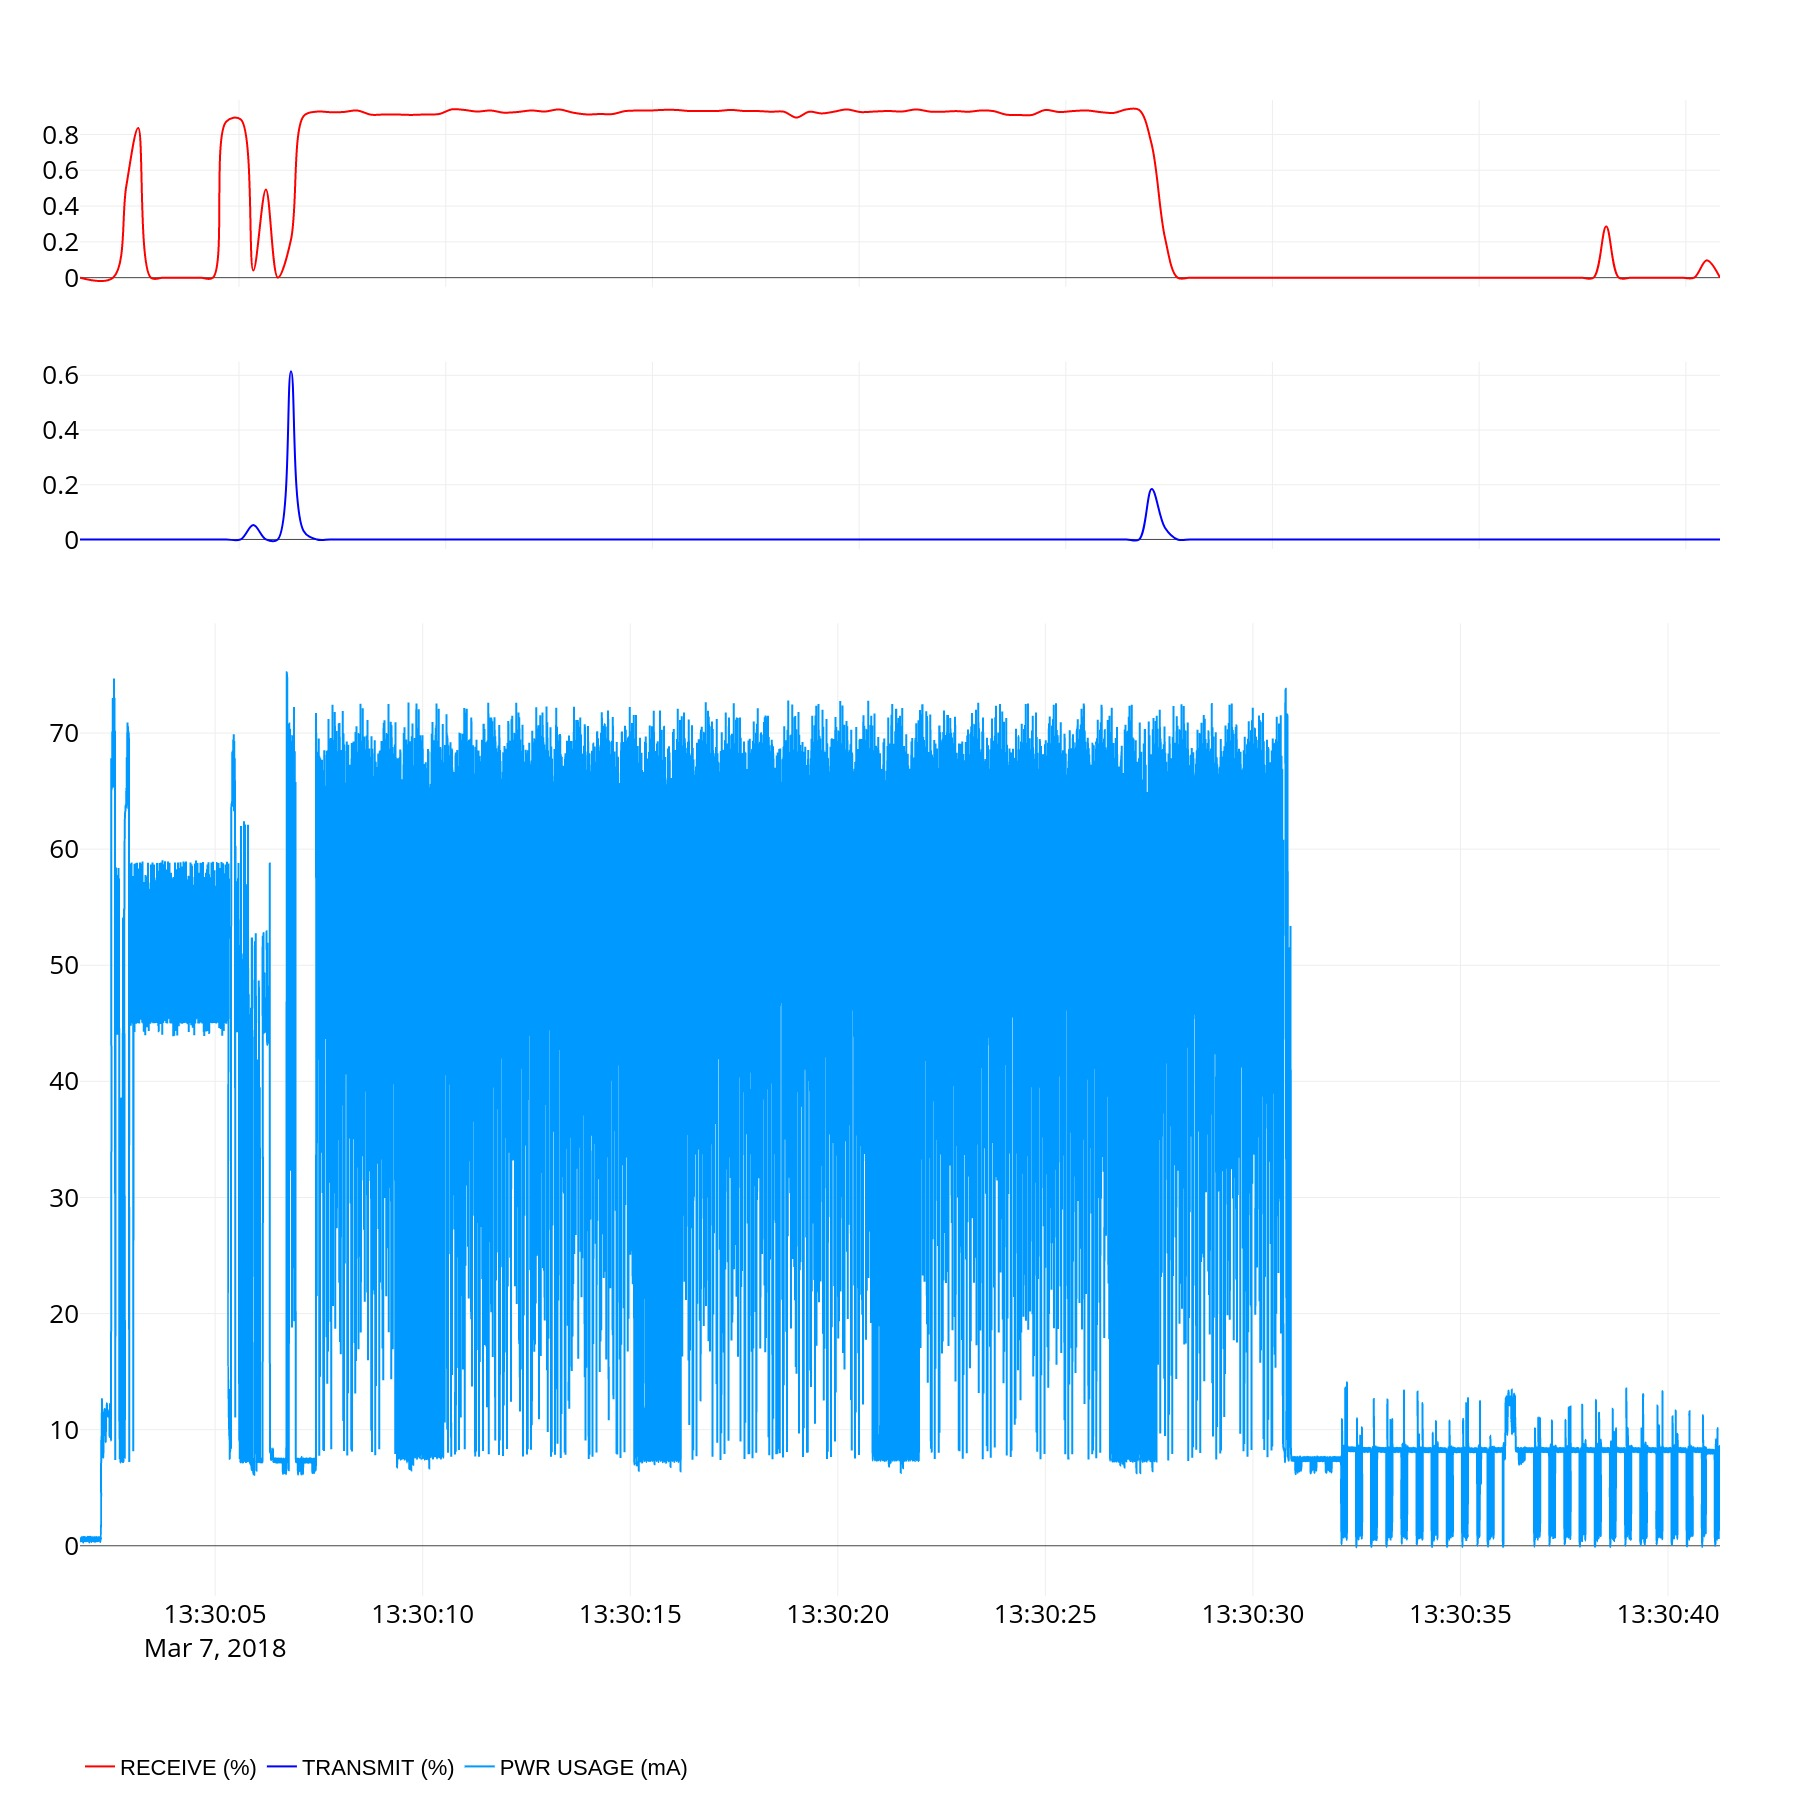
\includegraphics[width=0.9\textwidth, height=0.4\textheight]{/Users/henninghakonsen/Dropbox/Masteroppgave/thesis/latex/images/short_Q-FREE_TELENOR_5_02_2018-03-07_1_0x0_40_1_200.jpeg}
  \caption{1 x 40 Q-FREE, Telenor - device logging. See figure, \vref{figure:1x40_QFREE_TELENOR_1LOG}, or visit, \href{http://158.39.77.97:9000/\#/results/Q-FREE\_TELENOR\_5.02\_2018-03-07\_1\_0x0\_40\_1\_200}{webapp} \cite{online:result4}, for more details.}
  \label{figure:1x40_QFREE_TELENOR_1LOG_SHORT}
\end{figure}

Because of this bug we had some problems related to the long term tests so we had to investigate what actually happens when doing a longer test. The device would indicate network disconnection and reconnection, resulting in \acrshort{ecl} being 255 and receive/transmit counters were reset. We looked into the issue by monitoring the transmit process towards the server and most of the time the device did not try to reconnect to the network. The behavior is not expected and is most likely related to the hardware and software of the development kit. We conclude that the bug does introduce reconnection some times, but we believe it is hardware and software related and not network related. This is based on what we talked about in section, \vref{section:market}, that the chips produced at the point of the tests were not production ready, but good enough for us to test the networks.

\subsection{Coverage and \acrshort{ecl} level} \label{ssection:ecltest}
Depending on the devices signal power the \acrshort{ecl} level should adjust accordingly. As discussed in section, \acrshort{ecl} - \vref{ssection:ecl}, the network provider configures thresholds for \acrshort{ecl} levels and our results have mostly followed these thresholds as expected. We have included two figures to describe the behavior of different \acrshort{ecl} levels, \vref{figure:1x60_UIO_TELIA_ECL_0_SHORT} and \vref{figure:1x60_UIO_TELIA_ECL_2_SHORT}.
The two figures are showing results from one transmit of 50 bytes over a period of 60 with \acrshort{rai} set. You should focus on the two tops at the beginning of the figures, please visit the webapp(link is supplied in the figures) to zoom into the specific periods. If we begin looking at the first figure we can see that the signal power is good, but at transmit the power is bumped up from ${+9 \acrshort{dbm}}$ to ${+23 \acrshort{dbm}}$, maybe because of a \acrshort{nack}. Looking at the transmit graph we can see that the transmit process is relatively short, only covering approximately 1.5 seconds.
In addition we see that the device was actually only active for 15-20\% of that time, resulting in actual transmit time of \~0.3 seconds. We have used the program \textbf{power\_calculator.py} to calculate the power usage for the transmits and the following equation, \vref{equation:ecl0}, shows us the power usage of the transmit with \acrshort{ecl} level 0.

\begin{equation*} \label{equation:ecl0}
\begin{aligned}
From: 2018-03-16 12:35:55.901531 \\
To: 2018-03-16 12:35:57.543329 \\
((24.7694923857868\acrshort{ma} * 3.3V / 60 / 60 ) * 1.641798S) = 0.037278\acrshort{mwh} \\
\end{aligned}
\end{equation*}

This next figure is showing a transmit where the signal power is poor, hence the \acrshort{ecl} level is 2. Not surprisingly the transmit power is at ${+23 \acrshort{dbm}}$ and we can see a clear difference in this result compared to the previous. First of all the transmit process endures longer, around 5 seconds, hence the device is retransmitting the packet to ensure that it will be received at the \acrshort{enb}. The following equation, \vref{equation:ecl2}, shows us the power usage of the transmit with \acrshort{ecl} level 2.

\begin{equation*} \label{equation:ecl2}
\begin{aligned}
From: 2018-03-16 13:13:42.283327 \\
To: 2018-03-16 13:13:47.912613 \\
((80.83920204978038\acrshort{ma} * 3.3V / 60 / 60 ) * 5.629286S) = 0.417145\acrshort{mwh} \\
\end{aligned}
\end{equation*}

If we compare the two transmit operations we see that the second transmit uses \~11.2 times as much power as the first. In our experience the first transmit is the most accurate towards what actually is going on most of the time, but if the \acrshort{ue} has bad reception the battery lifetime will be heavily damaged. In section, \vref{ssection:transmitprocedure}, we described the theoretical disadvantage of different \acrshort{ecl} levels, however we think that this comparison is more accurate towards normal behavior. We have only included results from Telia for this observation since the results were very similar. We did not see the expected increase with very good reception at Q-Free with Telenor either, hence in practice the difference in power usage with "normal" reception is not millions of times higher.

\begin{figure}[H]
  \centering
  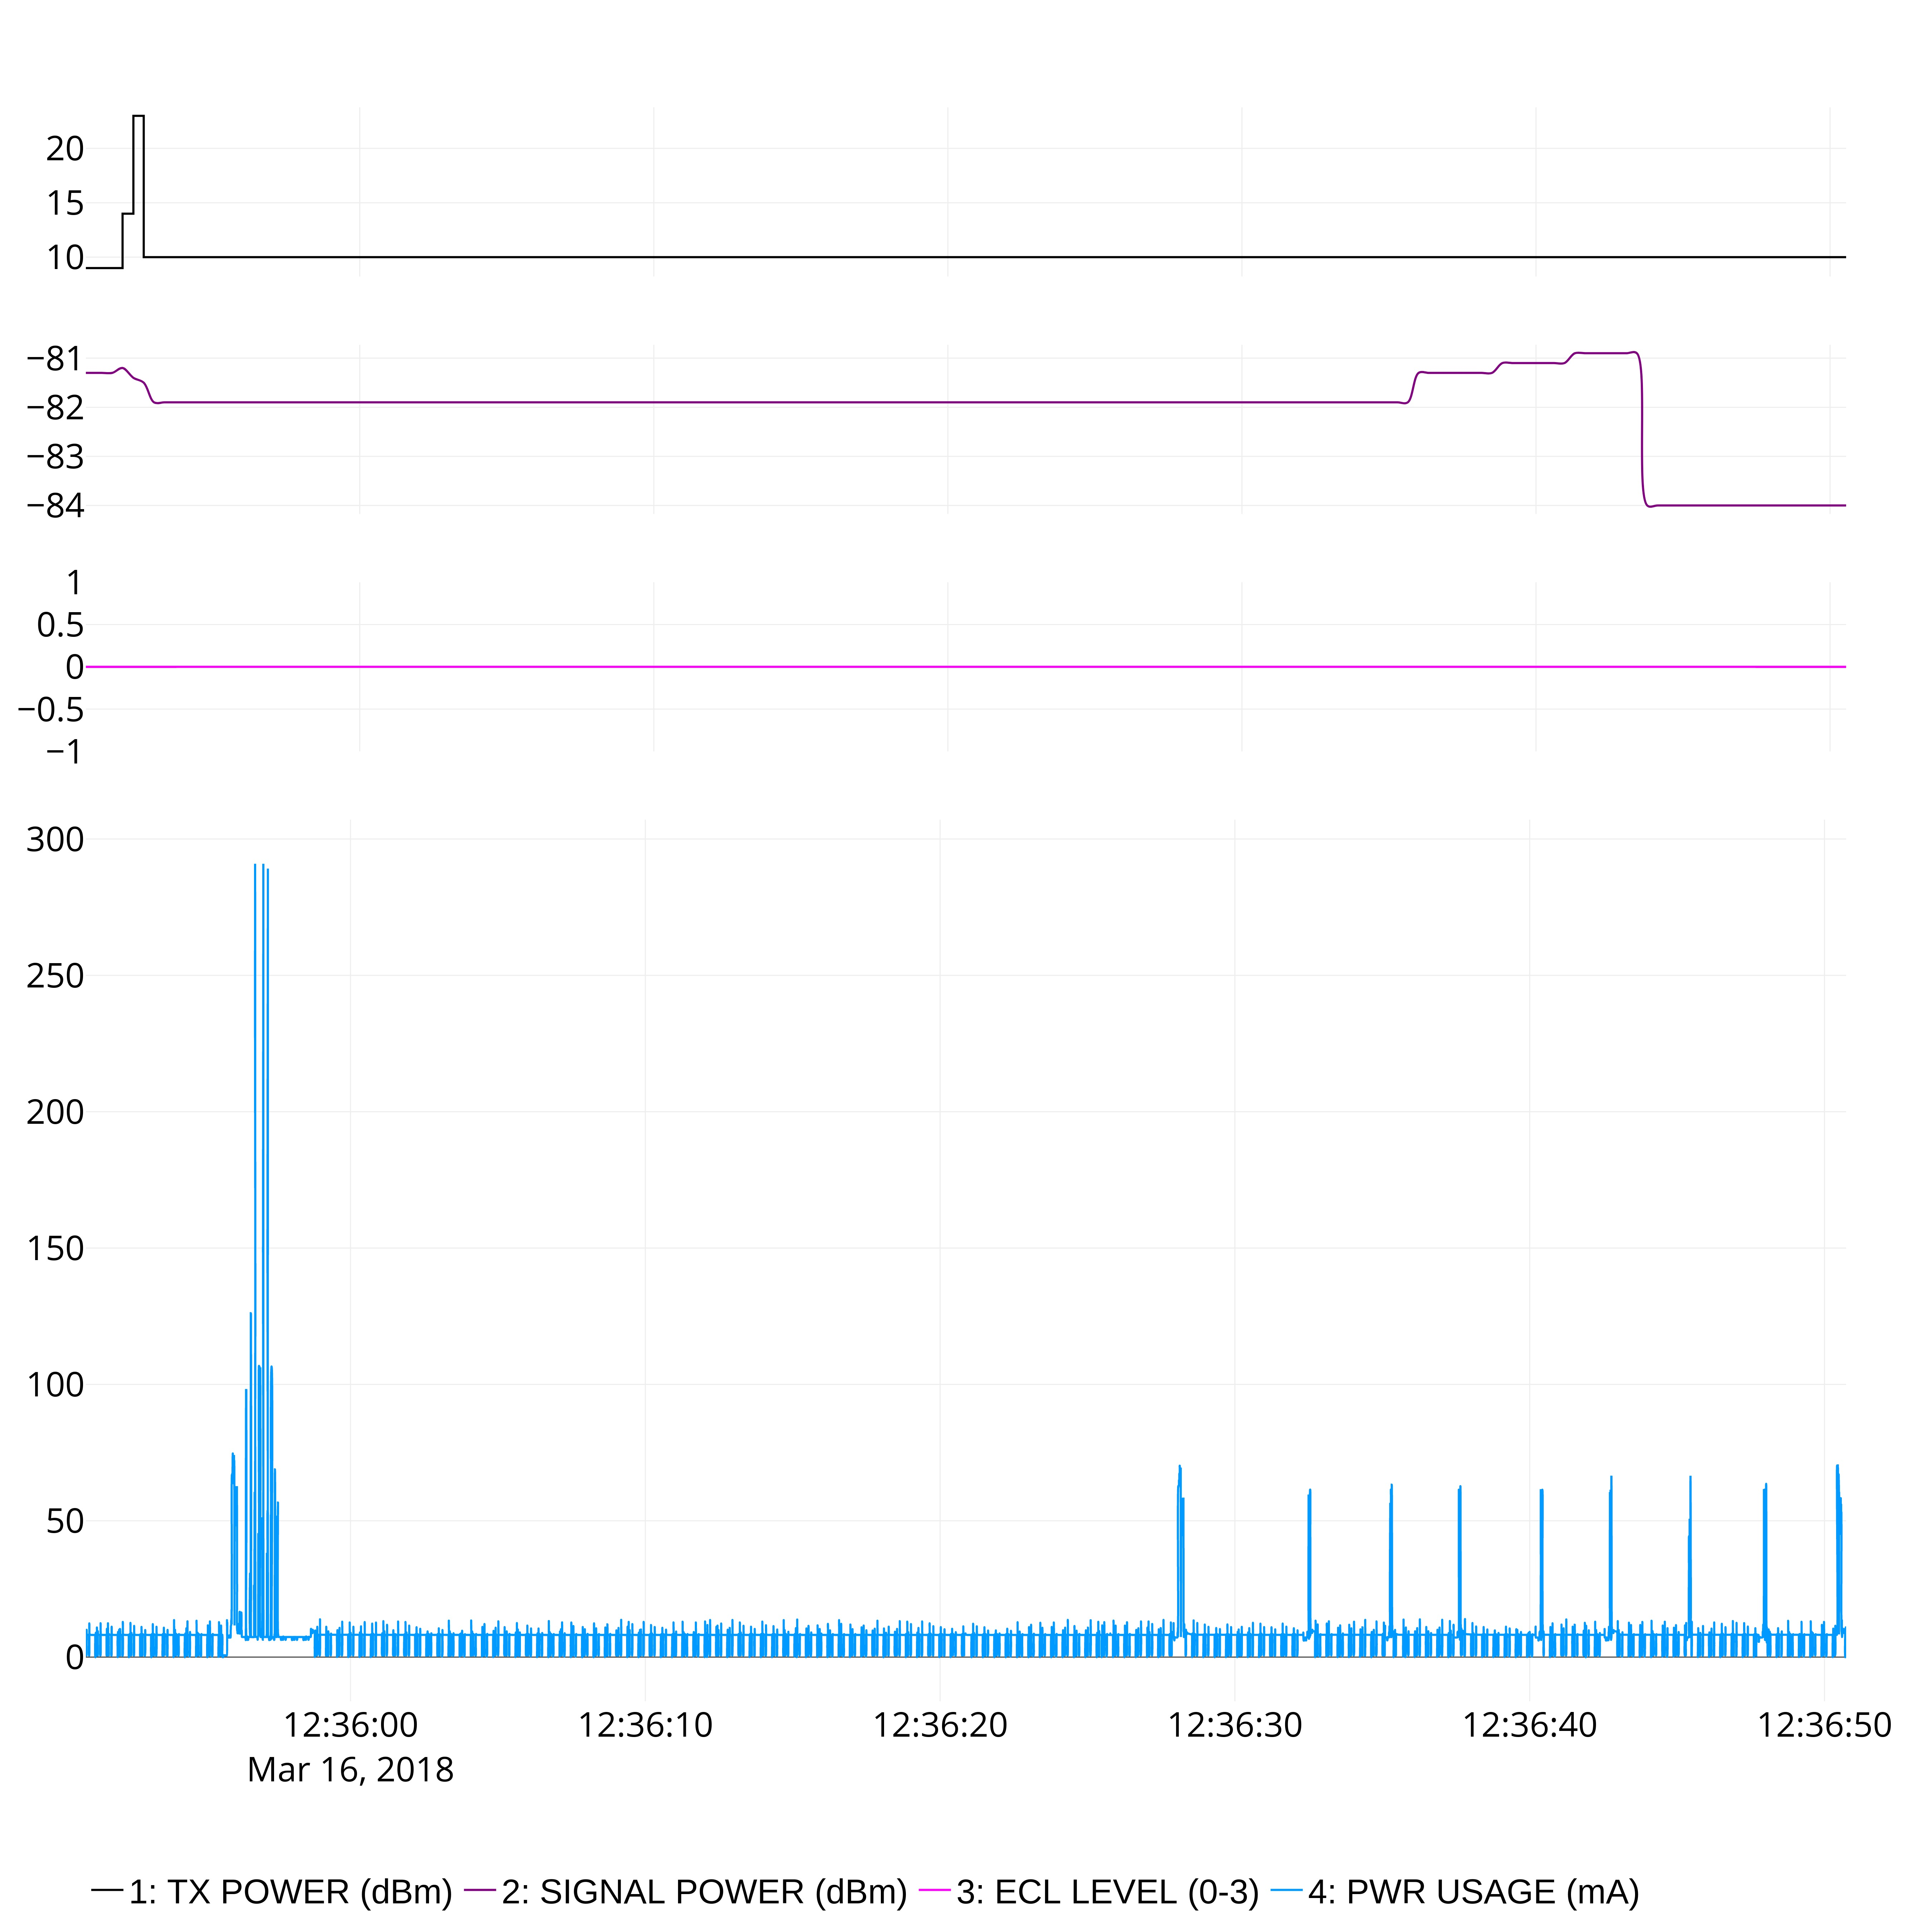
\includegraphics[width=0.9\textwidth, height=0.4\textheight]{/Users/henninghakonsen/Dropbox/Masteroppgave/thesis/latex/images/short_UiO_TELIA_5_02_precision_2018-03-16_1_0x2_60_1_50.jpeg}
  \caption{1 x 60 UiO, Telia - \acrshort{ecl} 0. See figure, \vref{figure:1x60_UIO_TELIA_ECL_0}, or visit, \href{http://158.39.77.97:9000/\#/results/UiO\_TELIA\_5.02\_precision\_2018-03-16\_1\_0x2\_60\_1\_50}{webapp} \cite{online:result5}, for more details.}
  \label{figure:1x60_UIO_TELIA_ECL_0_SHORT}
\end{figure}

\begin{figure}[H]
  \centering
  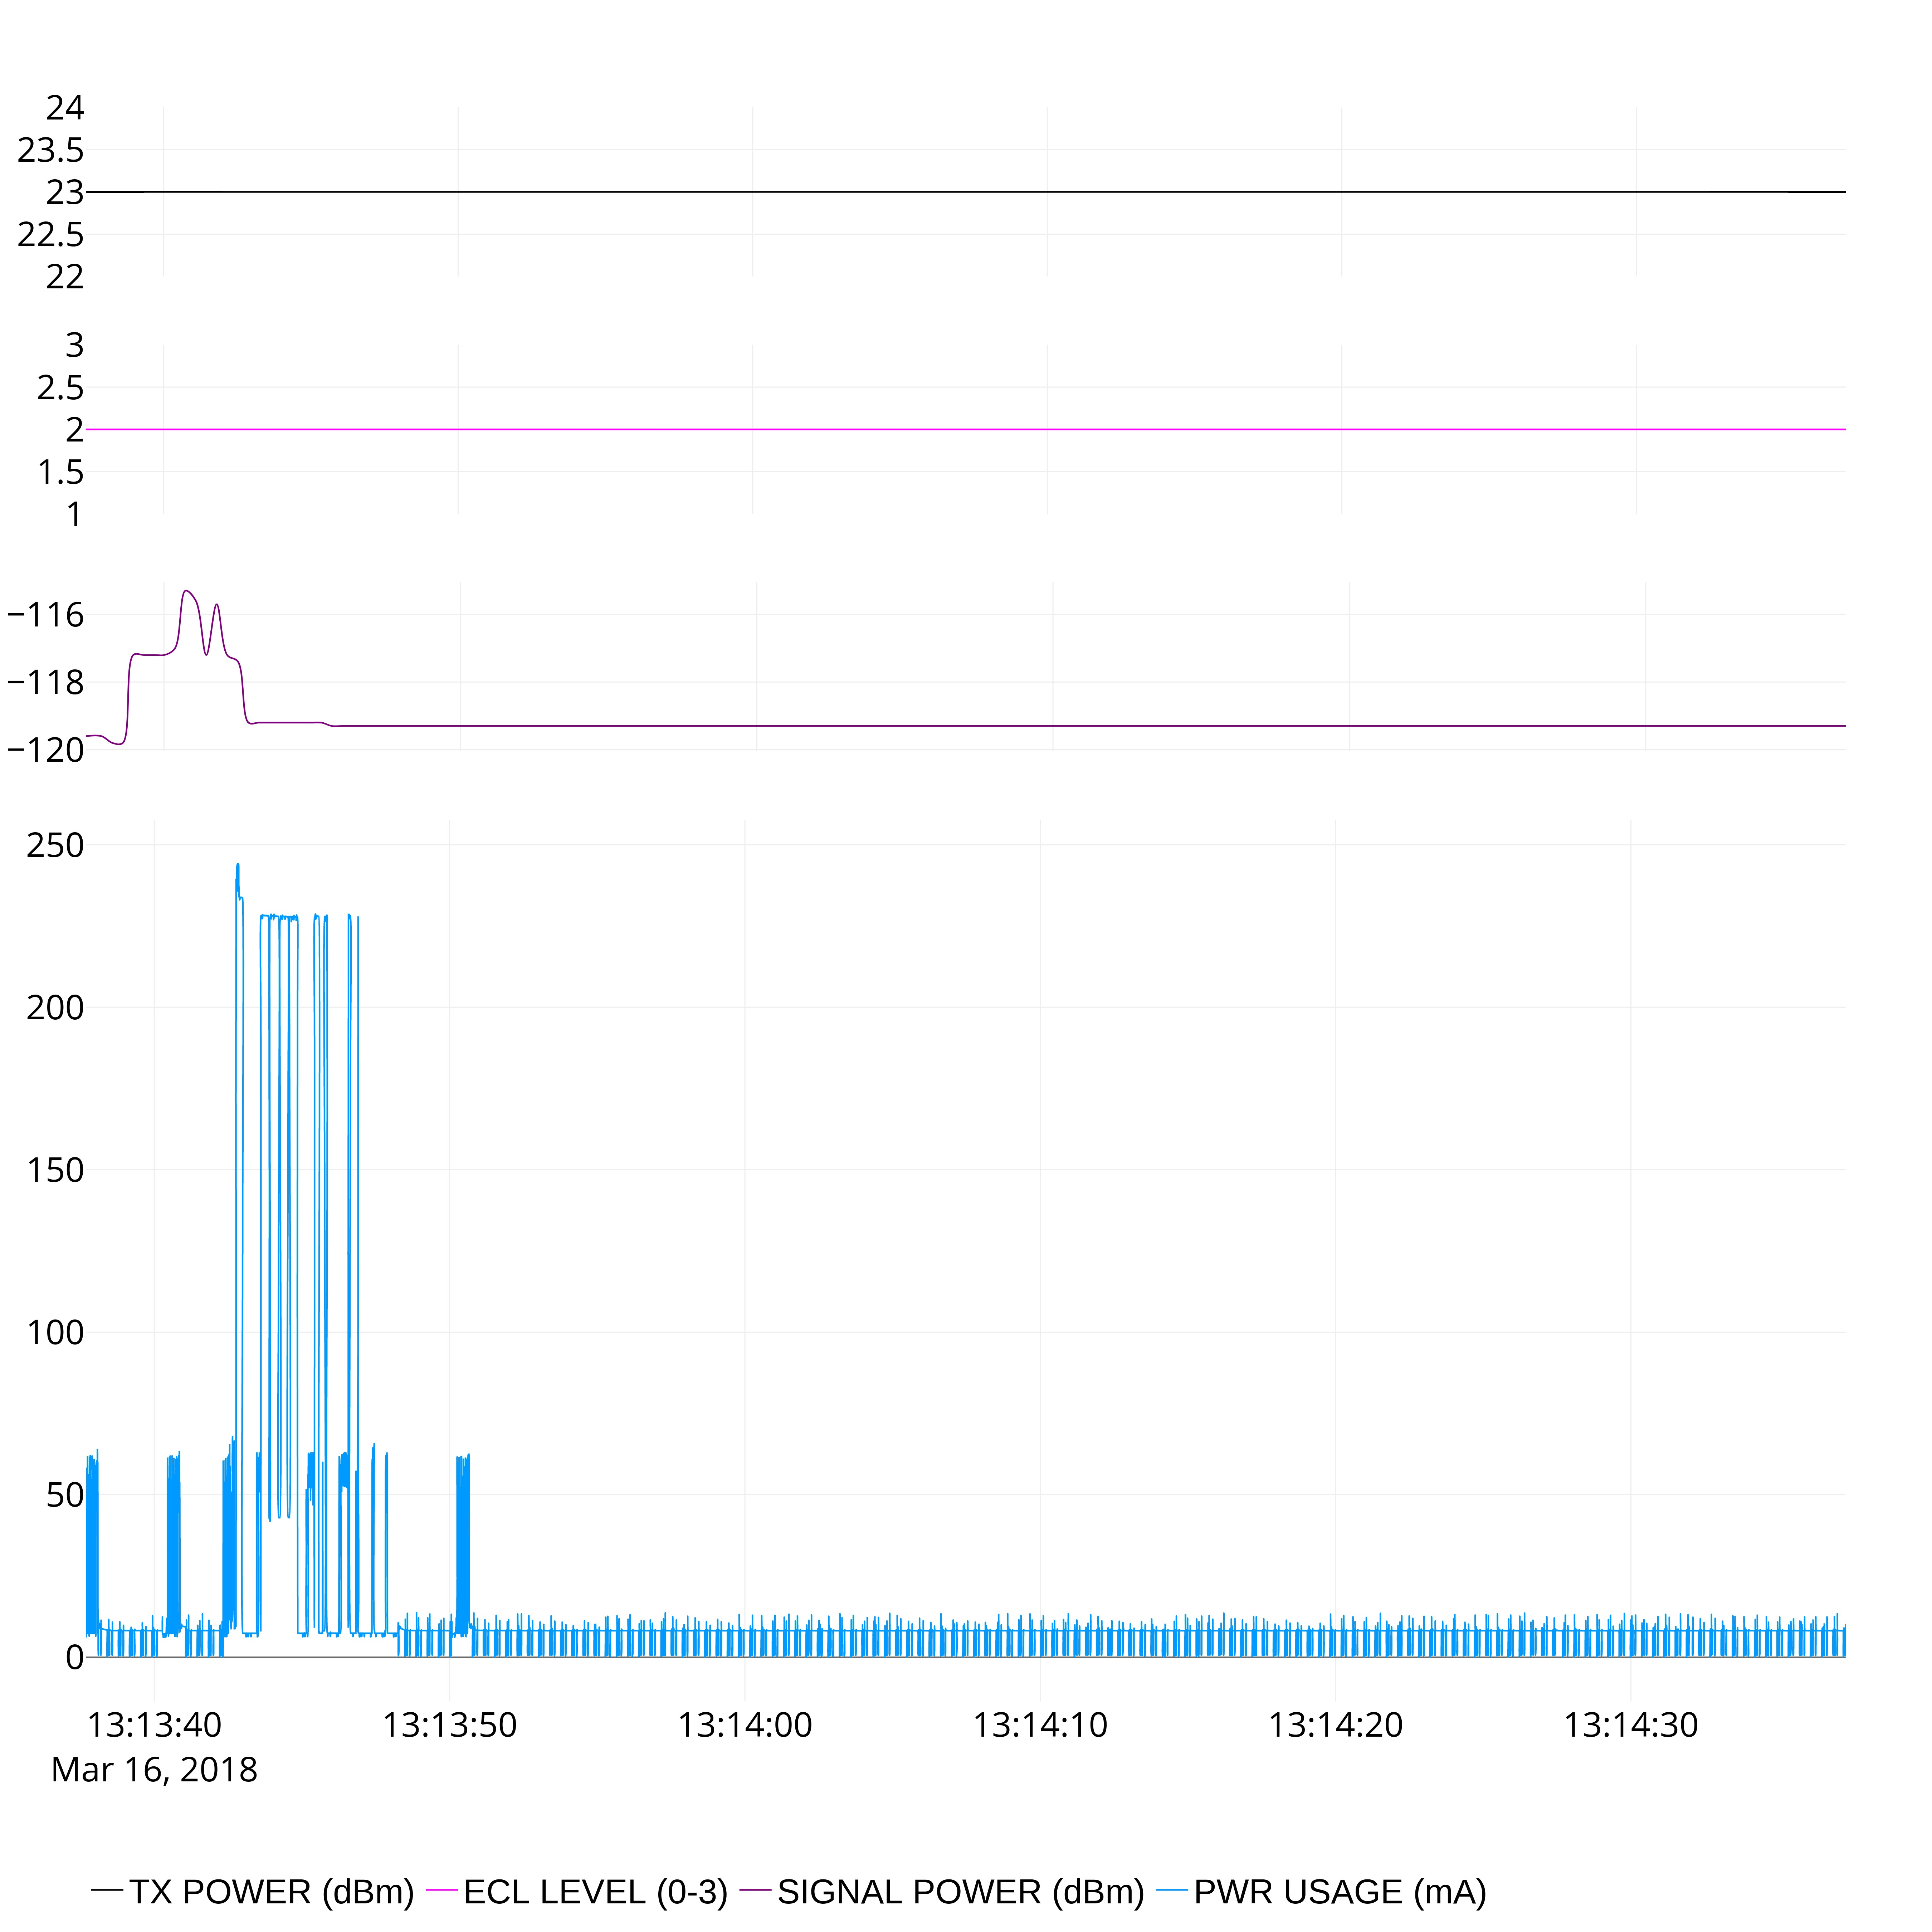
\includegraphics[width=0.9\textwidth, height=0.4\textheight]{/Users/henninghakonsen/Dropbox/Masteroppgave/thesis/latex/images/short_UiO_TELIA_5_02_precision_+30dBm_att_2018-03-16_1_0x2_60_1_50.jpeg}
  \caption{1 x 60 UiO, Telia - \acrshort{ecl} 2. See figure, \vref{figure:1x60_UIO_TELIA_ECL_2}, or visit, \href{http://158.39.77.97:9000/\#/results/UiO\_TELIA\_5.02\_precision\_+30dBm\_att\_2018-03-16\_1\_0x2\_60\_1\_50}{webapp} \cite{online:result6}, for more details.}
  \label{figure:1x60_UIO_TELIA_ECL_2_SHORT}
\end{figure}

\subsection{Transmit comparison}
We did a test where we sent packets from Q-Free's office towards Telia and Telenor with different packets sizes and at different coverage levels. This was a good opportunity to collect the results and compare the results in a chart. All transmits used the same setup and the signal power was altered using attenuators. One thing to note is that since the tests were performed at Q-Free where the signal power of Telenor's network is exceptional, the device never entered \acrshort{ecl} level 1 or 2 with Telenor's network. There was however an interesting result and we will begin looking at the results from the transmits without \acrshort{rai} set, \vref{figure:transmit_comparison_0}.

There are a few things to notice in this chart. First of all there are two groupings, one with Telenor's transmits and another with Telia's. As we have seen before Telia's transmits use less time in RRC mode, hence lowering the power usage. We see that Telia uses around 50\% less power at the first two transmits, regardless of byte size. It is not until the last transmit where Telia's transmits uses more power, and this is because the device has entered \acrshort{ecl} level 2 and retransmits occurs.
We will look closer into packet size in the next section, \vref{ssection:packetsize}, but we can see indications that packet sizes does influence the power usage to some degree.

Moving over to the chart with transmits with \acrshort{rai} set we see that the results are more similar between the two network providers when the device is in \acrshort{ecl} level 0. If we look closely at the first transmits from Telia we can see a bigger gap between packet sizes, and this is mainly because the RRC period is not influencing the results and we get more information about the actual transmit process.
You can view the actual transmit graphs at \url{henninghaakonsen.me} where they are tagged with \textbf{60\_1}.

\begin{figure}[H]
  \centering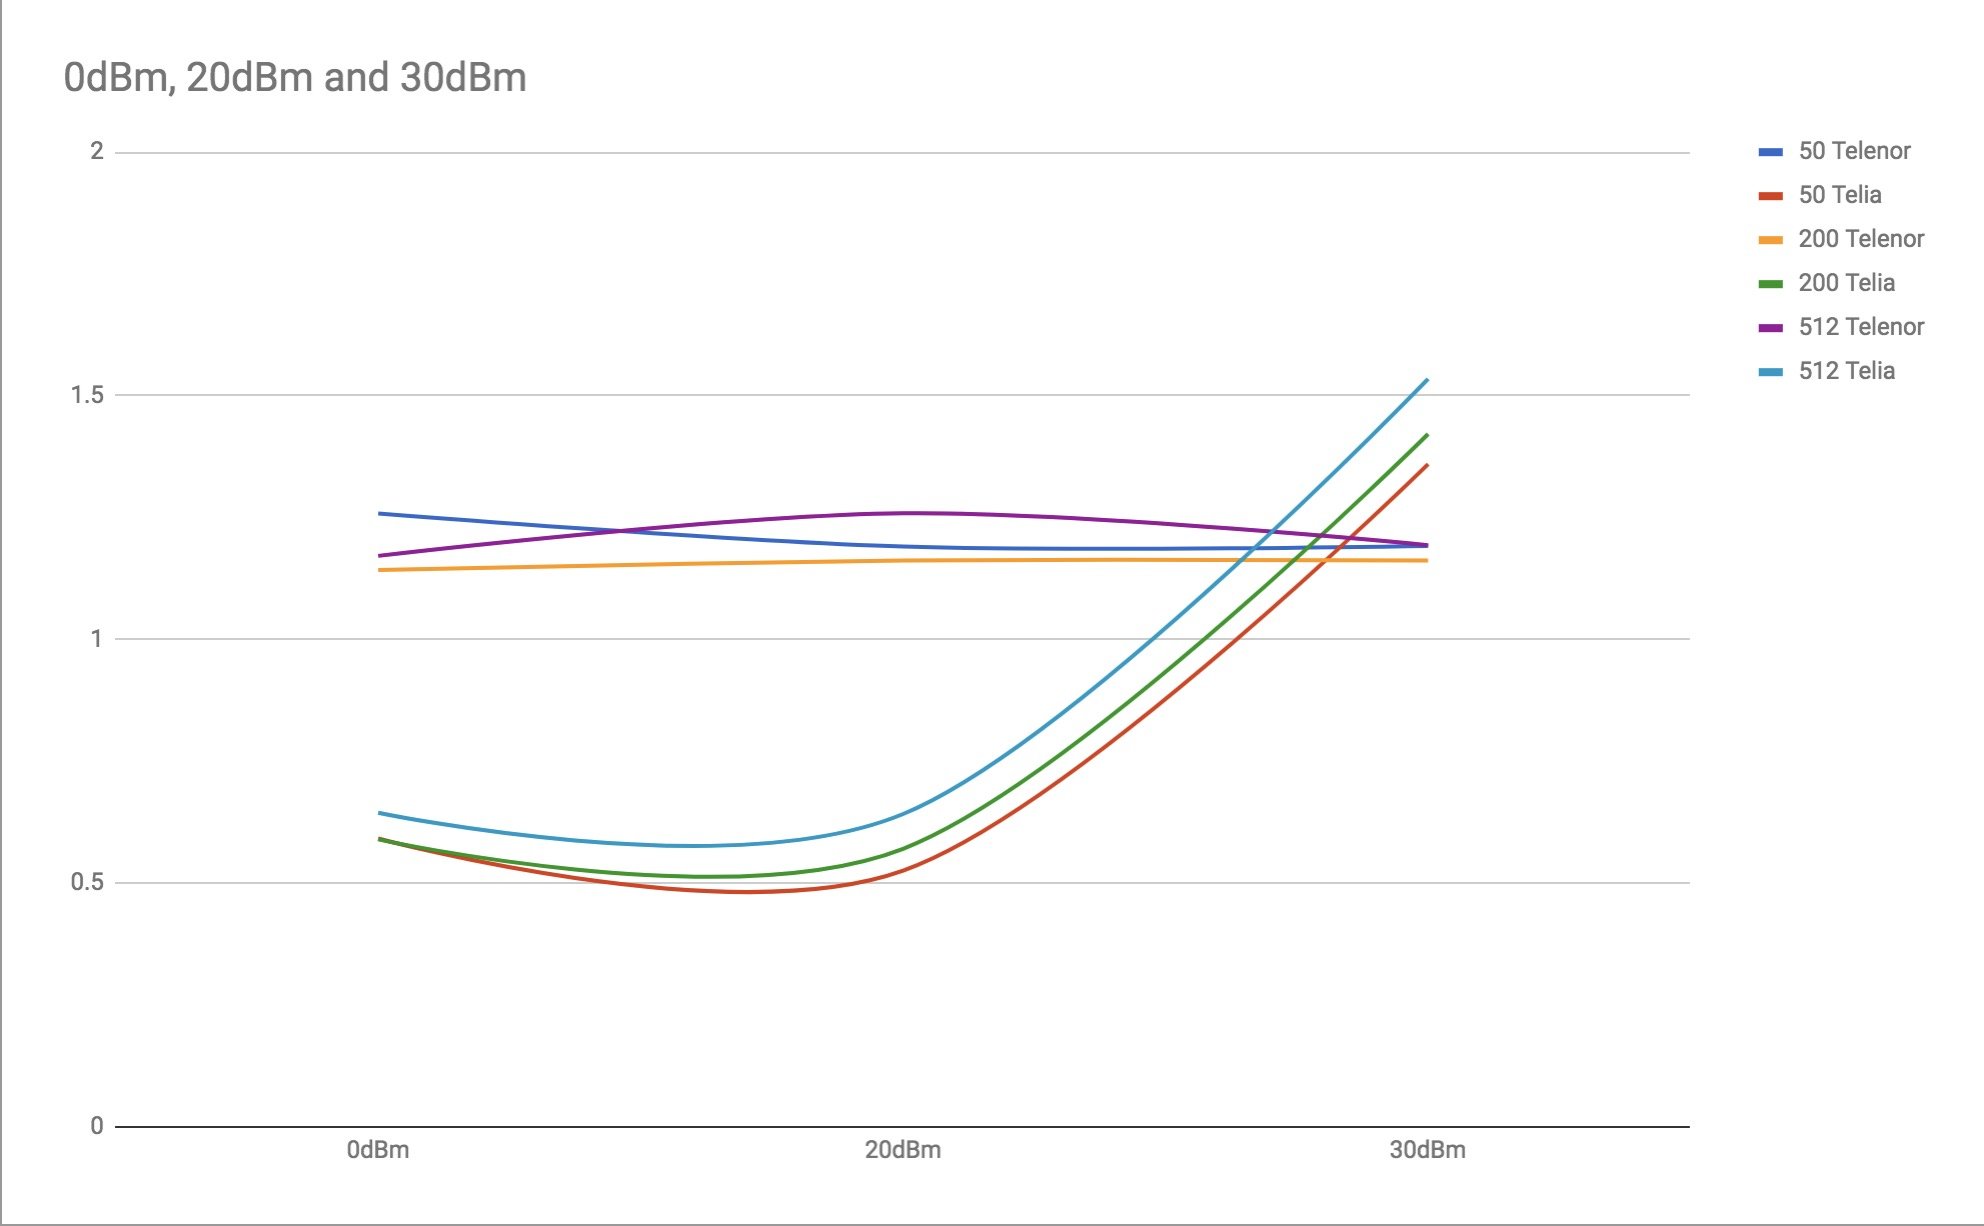
\includegraphics[width=\textwidth,height=8cm]{/Users/henninghakonsen/Dropbox/Masteroppgave/thesis/latex/images/transmitcomparison_0}
  \caption{Transmit comparison without \acrshort{rai}}
  \label{figure:transmit_comparison_0}
\end{figure}

\begin{figure}[H]
  \centering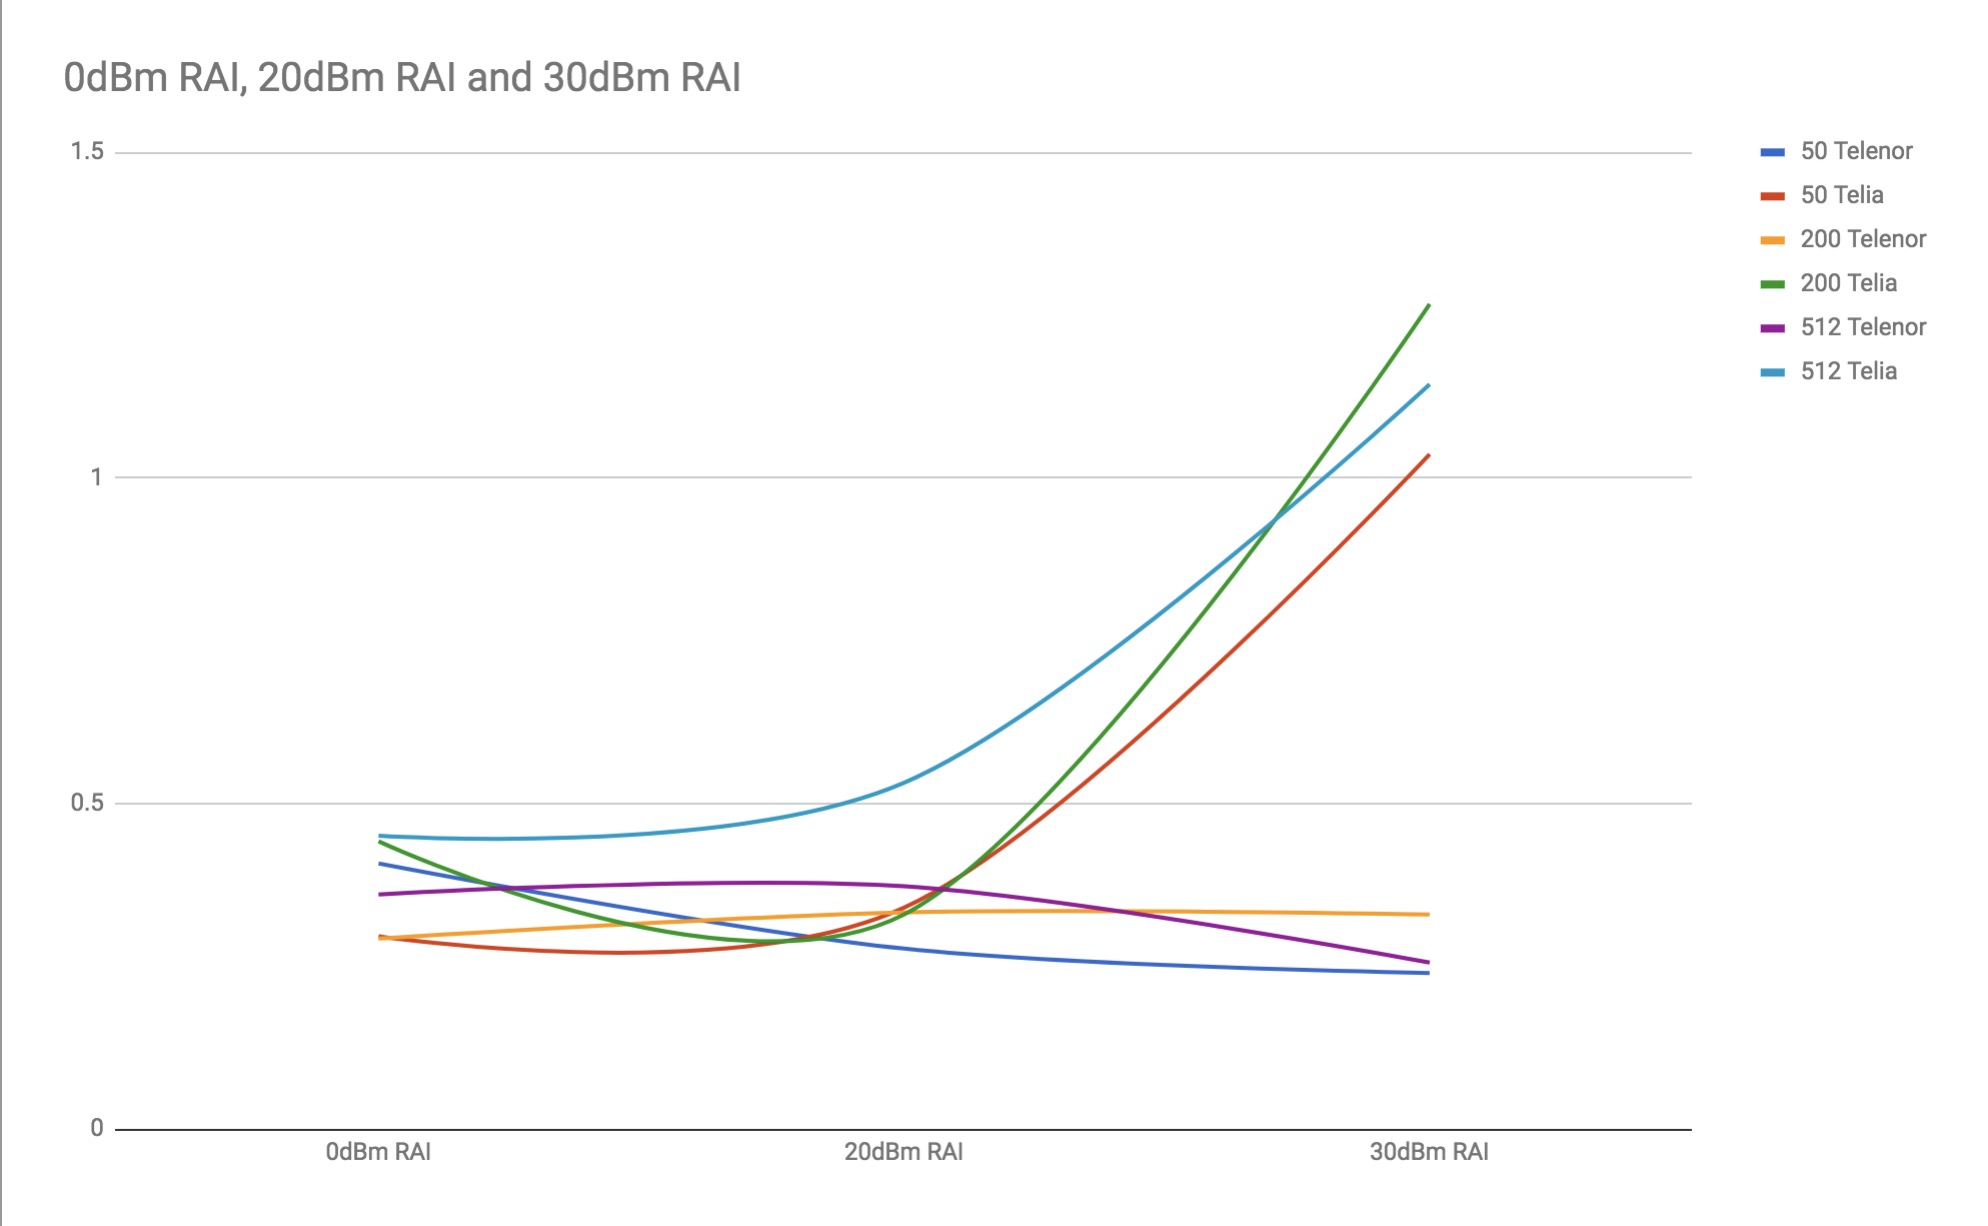
\includegraphics[width=\textwidth,height=8cm]{/Users/henninghakonsen/Dropbox/Masteroppgave/thesis/latex/images/transmitcomparison_1}
  \caption{Transmit comparison with \acrshort{rai}}
  \label{figure:transmit_comparison_1}
\end{figure}

\subsection{Packet size} \label{ssection:packetsize}
The typical packet size for an \acrshort{iot} device is often small, typically under 100 bytes, but for some cases bigger packets might be required and we have performed a specific test to see what the packet size does with a transmit. The test is performed with the program \textbf{nbiot\_labtest\_details.py} and a list of parameters is described in table, \vref{table:labtest_details_parameters}.

\begin{table}[H]
\centering
\resizebox{\textwidth}{!}{%
\begin{tabular}{|l|m{10cm}|}
  \hline
  \textbf{Parameter} & \textbf{Description} \\ \hline
  -gn & Output graph name. The supplied name will lead the heading, followed by a list of the rest of the parameters. \\ \hline
  -d & Set the desired delay between each iteration. Default: 5 \\ \hline
  -i & Set the desired iterations. \\ \hline
  -r & Set \acrshort{rai}. Default: false \\ \hline
\end{tabular}%
}
\caption{\textbf{nbiot\_labtest\_details.py} parameters}
\label{table:labtest_details_parameters}
\end{table}

Depending on the parameters passed to the program it will transmit a number of packets with different sizes - 25, 50, 100, 200, 400 and 512. After all transmits are finished the program will produce two graphs, one with all transmits on the left and another on the right with statistics about all transmits. We have included average, sum, min and max of all transmits, categorized by packet size. This is the graph which you should focus on, since this is displaying aggregated data which gives us a better overview of the transmit process. We have included two figures in section, \vref{figure:details_0} and \vref{figure:details_1}, which displays two executions of the program - one with \acrshort{rai} and one without. We needed to test both transmit modes to see how much the transmit process with different packet sizes costs in terms of power usage.

We begin looking at the first figure - transmits without \acrshort{rai}. The whole transmit process without \acrshort{rai} endures approximately 20-30 seconds, while the actual transmit process only takes 0.5-2 seconds depending on the coverage level. Looking at all aggregated lines to the right it is easy to see that the bigger part of the power consumption comes from overhead of the RRC process. There is a slight increase in power usage while increasing the packet size, but it is clear that if your application transmits packets without \acrshort{rai} flag the packet size is not crucial to the power usage.

Moving over to the next graph we see a noticeable difference. Not surprisingly there is a general decrease in power usage when using \acrshort{rai}. If we look at the average aggregated value of packets transmitted with 25 bytes, there is a decrease of 240\%. This results in less overhead from other processes related to the transmit, hence the power usage from the transmit has bigger influence on the graphs. Looking at the average line in pink there is a steady increase in power usage related to the packet size. Comparing 25 and 512 bytes, there is a power increase of 217\% which sounds logical since a bigger payload required several data packets. It is interesting to look at the aggregated sum of each byte size category. According to, \cite{online:rohde}, the \acrfull{mps} is 680 bits, which is 85 bytes. Looking at the aggregated sum line we see two spikes which is likely to be related to the \acrshort{mps}. We can see the start of a spike at 100 bytes, which is directly after the \acrshort{mps}. There is another spike from 400 to 512 bytes, which also may be related to the maximum transmit size of the chip which is 512 bytes.

\begin{figure}[H]
  \centering
  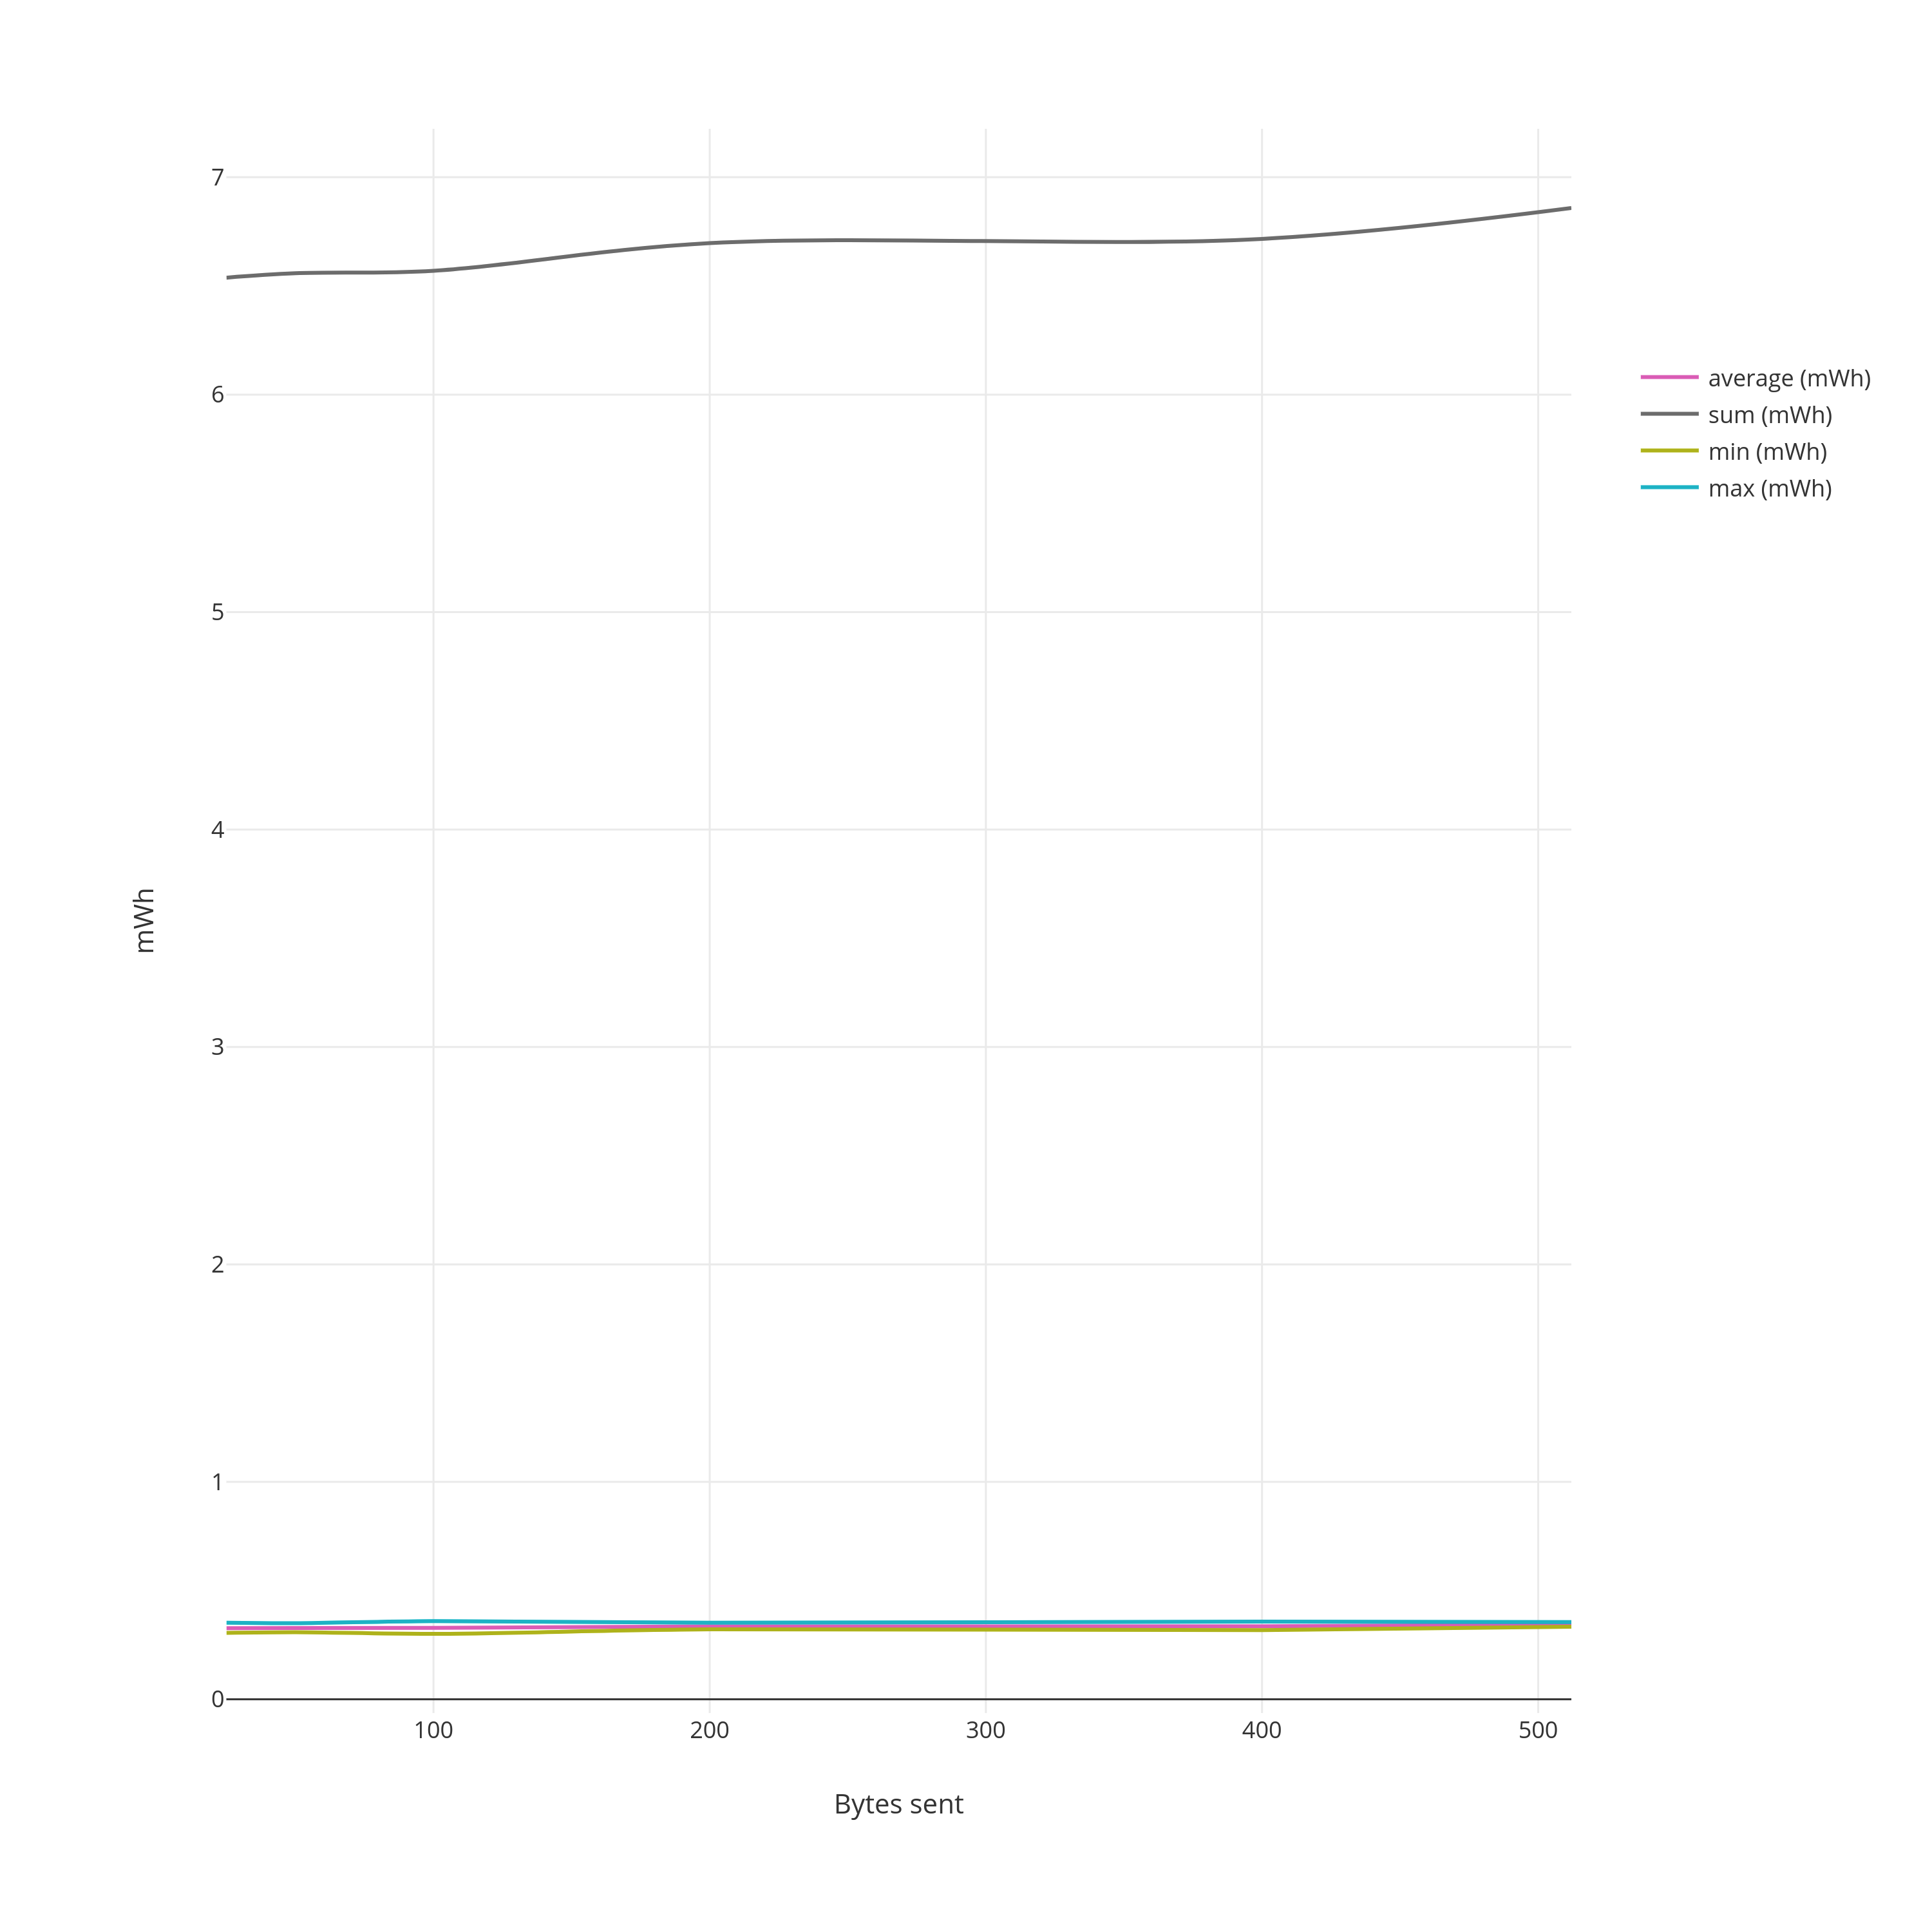
\includegraphics[width=0.9\textwidth, height=0.4\textheight]{/Users/henninghakonsen/Dropbox/Masteroppgave/thesis/latex/images/details_0.png}
  \caption{Details - \acrshort{rai} unset. Visit, \href{http://158.39.77.97:9000/\#/results/UiO\_TELIA\_long\_term\_2018-03-22\_0x0\_30\_20}{webapp} \cite{online:result7}, for more details.}
  \label{figure:details_0}
\end{figure}

\begin{figure}[H]
  \centering
  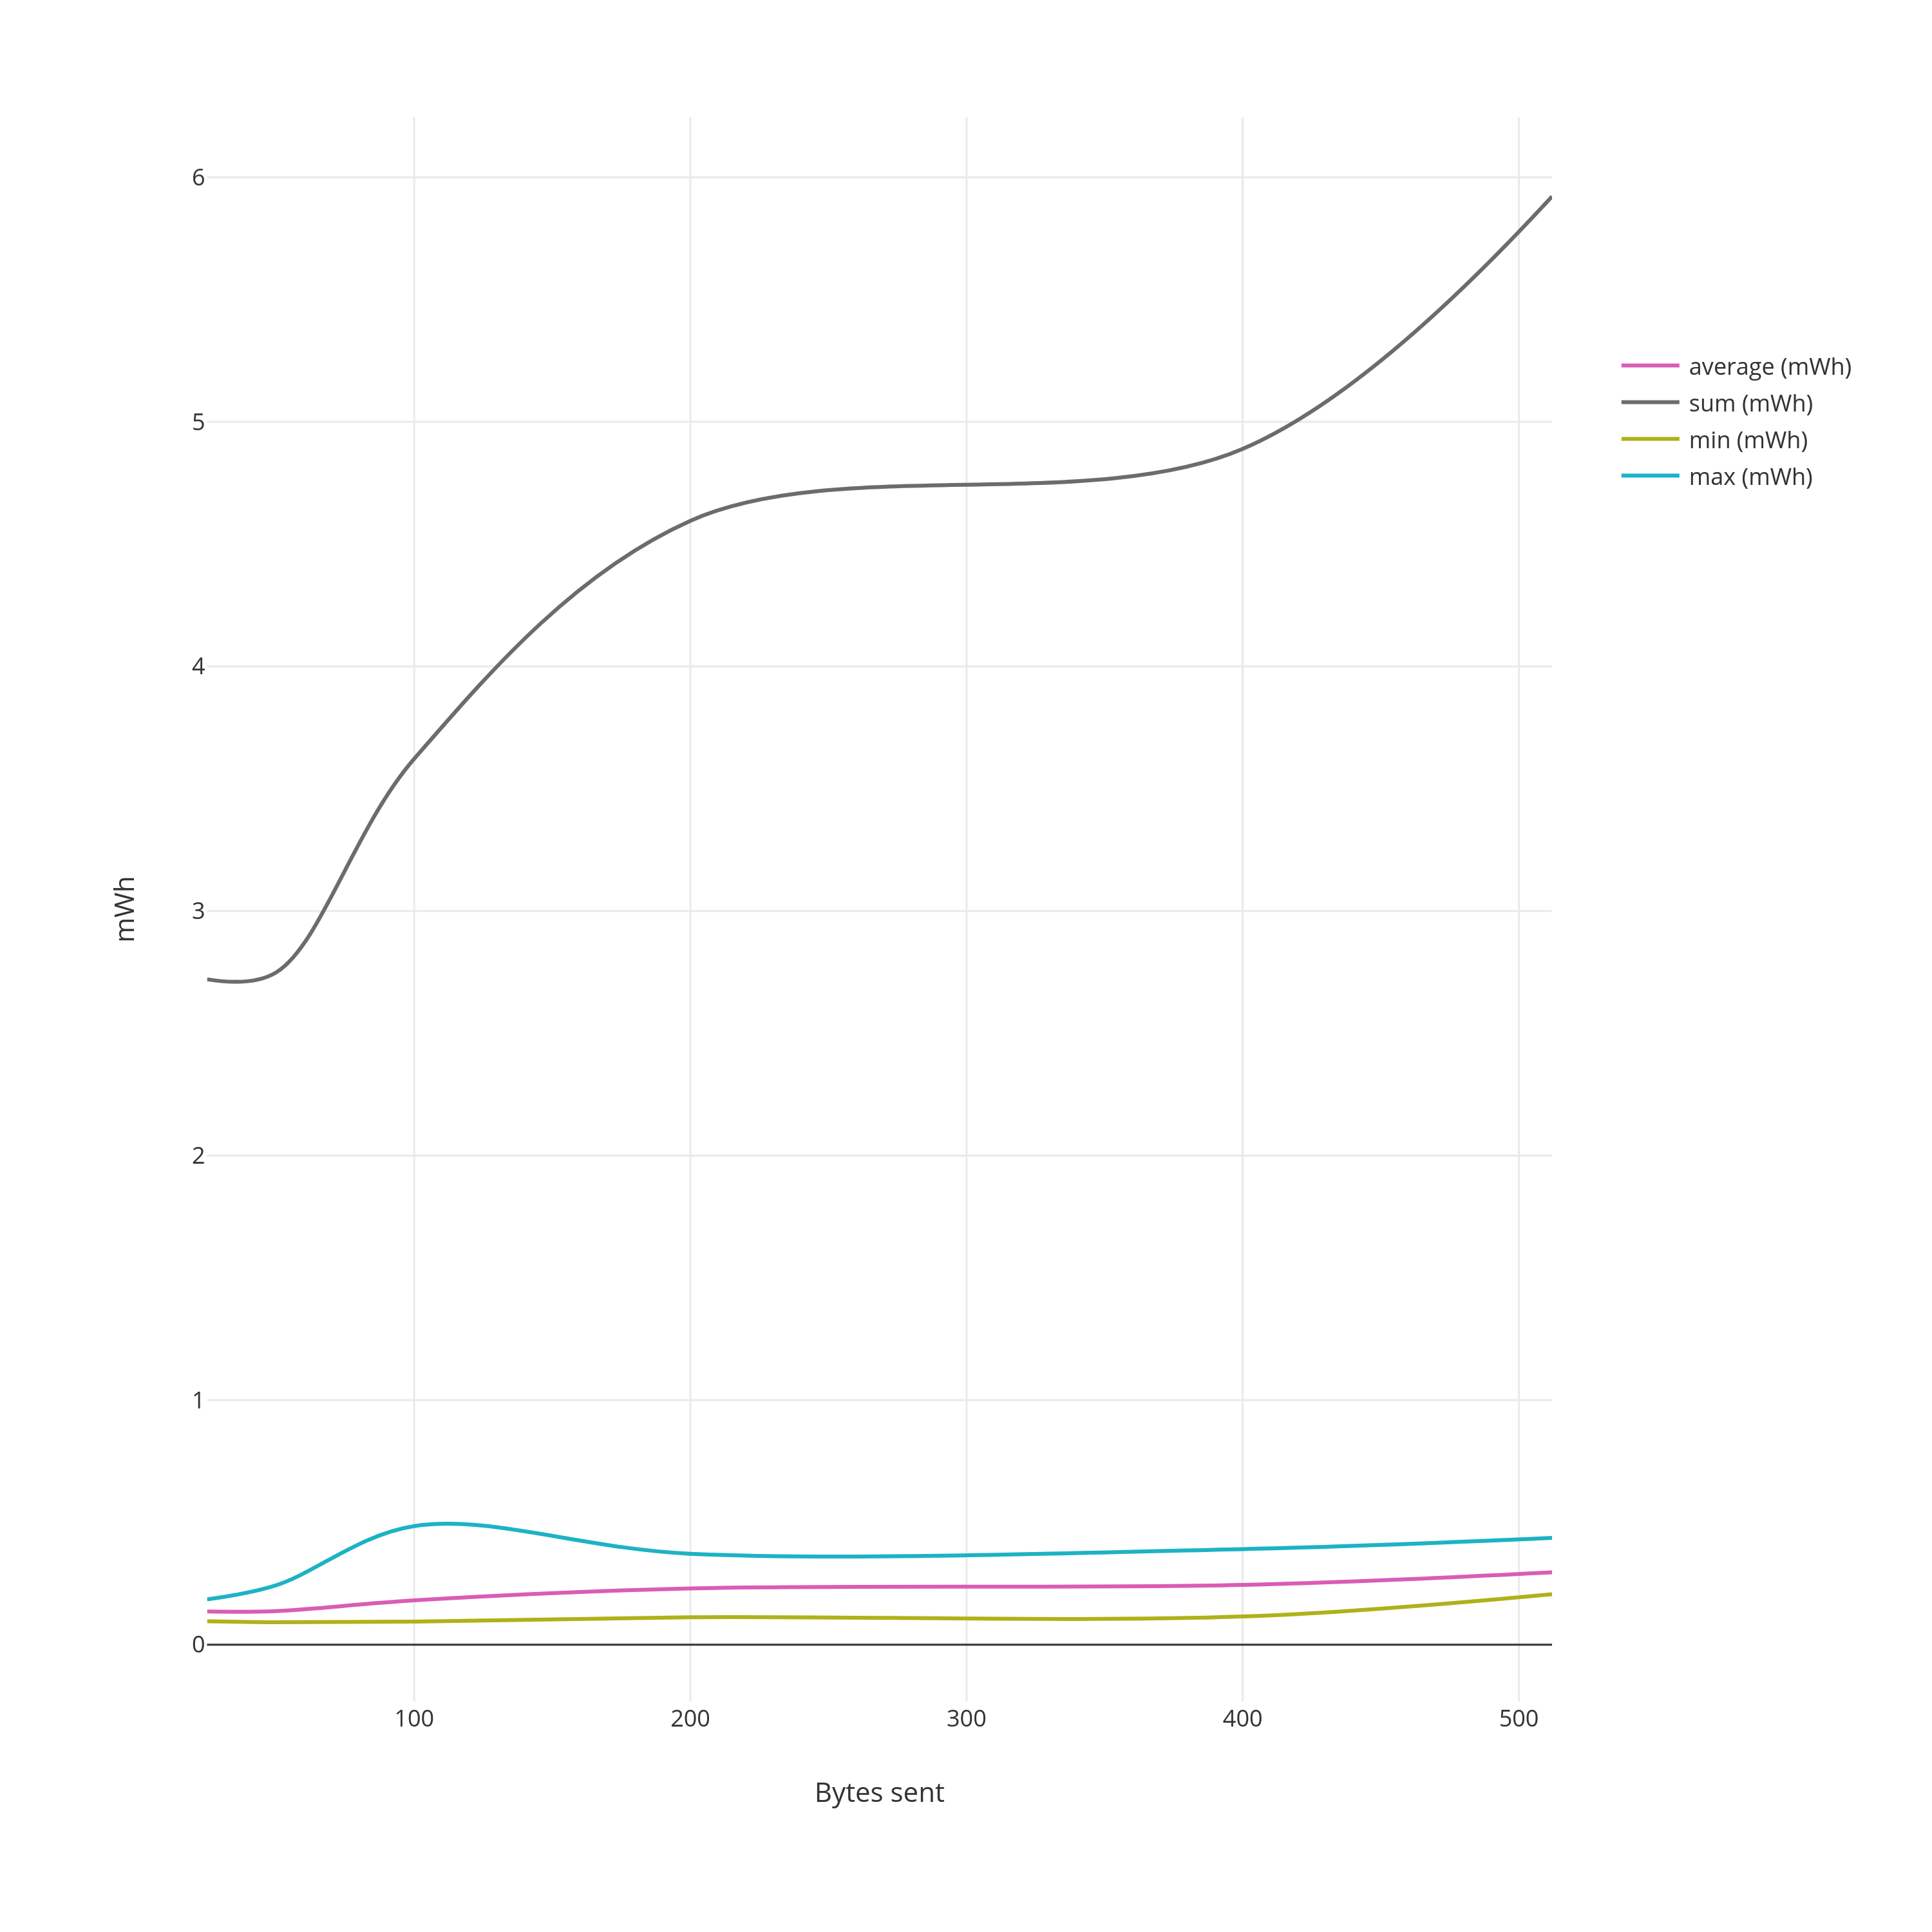
\includegraphics[width=0.9\textwidth, height=0.4\textheight]{/Users/henninghakonsen/Dropbox/Masteroppgave/thesis/latex/images/details_1.png}
  \caption{Details - \acrshort{rai} set.  Visit, \href{http://158.39.77.97:9000/\#/results/UiO\_TELIA\_long\_term\_2018-03-22\_0x2\_30\_20}{webapp} \cite{online:result8}, for more details.}
  \label{figure:details_1}
\end{figure}

\subsection{Sensor reboot} \label{ssection:reboottest}
There are a number of reasons why the device would perform a reboot, especially if the application is long term over several years. One reason for a reboot is because of some software or hardware fault, which could occur even though it should not happen. Another reason is that the developer reboots the device if it has stalled or some logic kicks in. The main reason to investigate what happens in a reboot is to see how long to network connection takes. If this process is long and cumbersome it will affect the power usage, hence the battery lifetime decreases. We will elaborate why and when your application should consider rebooting the device in section, \vref{section:guidelines}.

We performed several reboot tests - with both network providers and with different coverage levels. We have included two results, one from Telenor and one from Telia. The results supplied are very similar to the other tests we did with less good reception. The only difference was a slight increase in power consumption.
Since the device reboots we are not able to log the status of the device with \textbf{NUESTATS} so you will only be able to see the power usage in this test.

We will begin looking at Telenor's result without any attenuators - see figure \vref{figure:telenor_reboot}. The graph displays 120 seconds which includes the whole process of rebooting and connecting to the network. The first thing we see is a long period of what looks like RRC mode. Following is what looks like the actual connection process about half way into the graph and ending with a RRC period until the timer runs out and the device enters \acrshort{psm} mode. The whole process uses ${~5.1 \acrshort{mwh}}$, which if we use the results from the test about packet sizes is the same as around 28 transmits with 100 bytes payload with \acrshort{rai} set. If we assume that we transmit a packet every hour this reboot process uses approximately the same amount of power as a days worth of uptime uses.

Moving over to Telia's result without any attenuators, figure \vref{figure:telia_reboot}, you might notice that this result only covers 60 seconds. This is because the reboot process using Telia's network was much shorter and since we only want to look at the reboot process the log duration is kept to the minimum. Directly after reboot the device performs a set of transmits, followed by a period with RRC mode. After this process the device enters \acrshort{psm} and the device has connected to the network. The whole process uses ${0.55 \acrshort{mwh}}$, which is around ten times less than with Telenor's network. It is interesting to see the differences the network provider introduces to the network connection process, since this is mainly due to network configurations. One explanation of the lower power consumption is likely related to the power consumption during the RRC period. We saw in section, \vref{ssection:generaltest}, that Telia used around 60\% less time in RRC mode, hence reducing the power consumption drastically. In addition we see that the duration of the connection process is twice as long with Telenor. The results are consistent throughout all reboot tests and gives an indication that Telia has used the configuration to reduce the power consumption on reboot and in these RRC periods.

\begin{figure}[H]
  \centering
  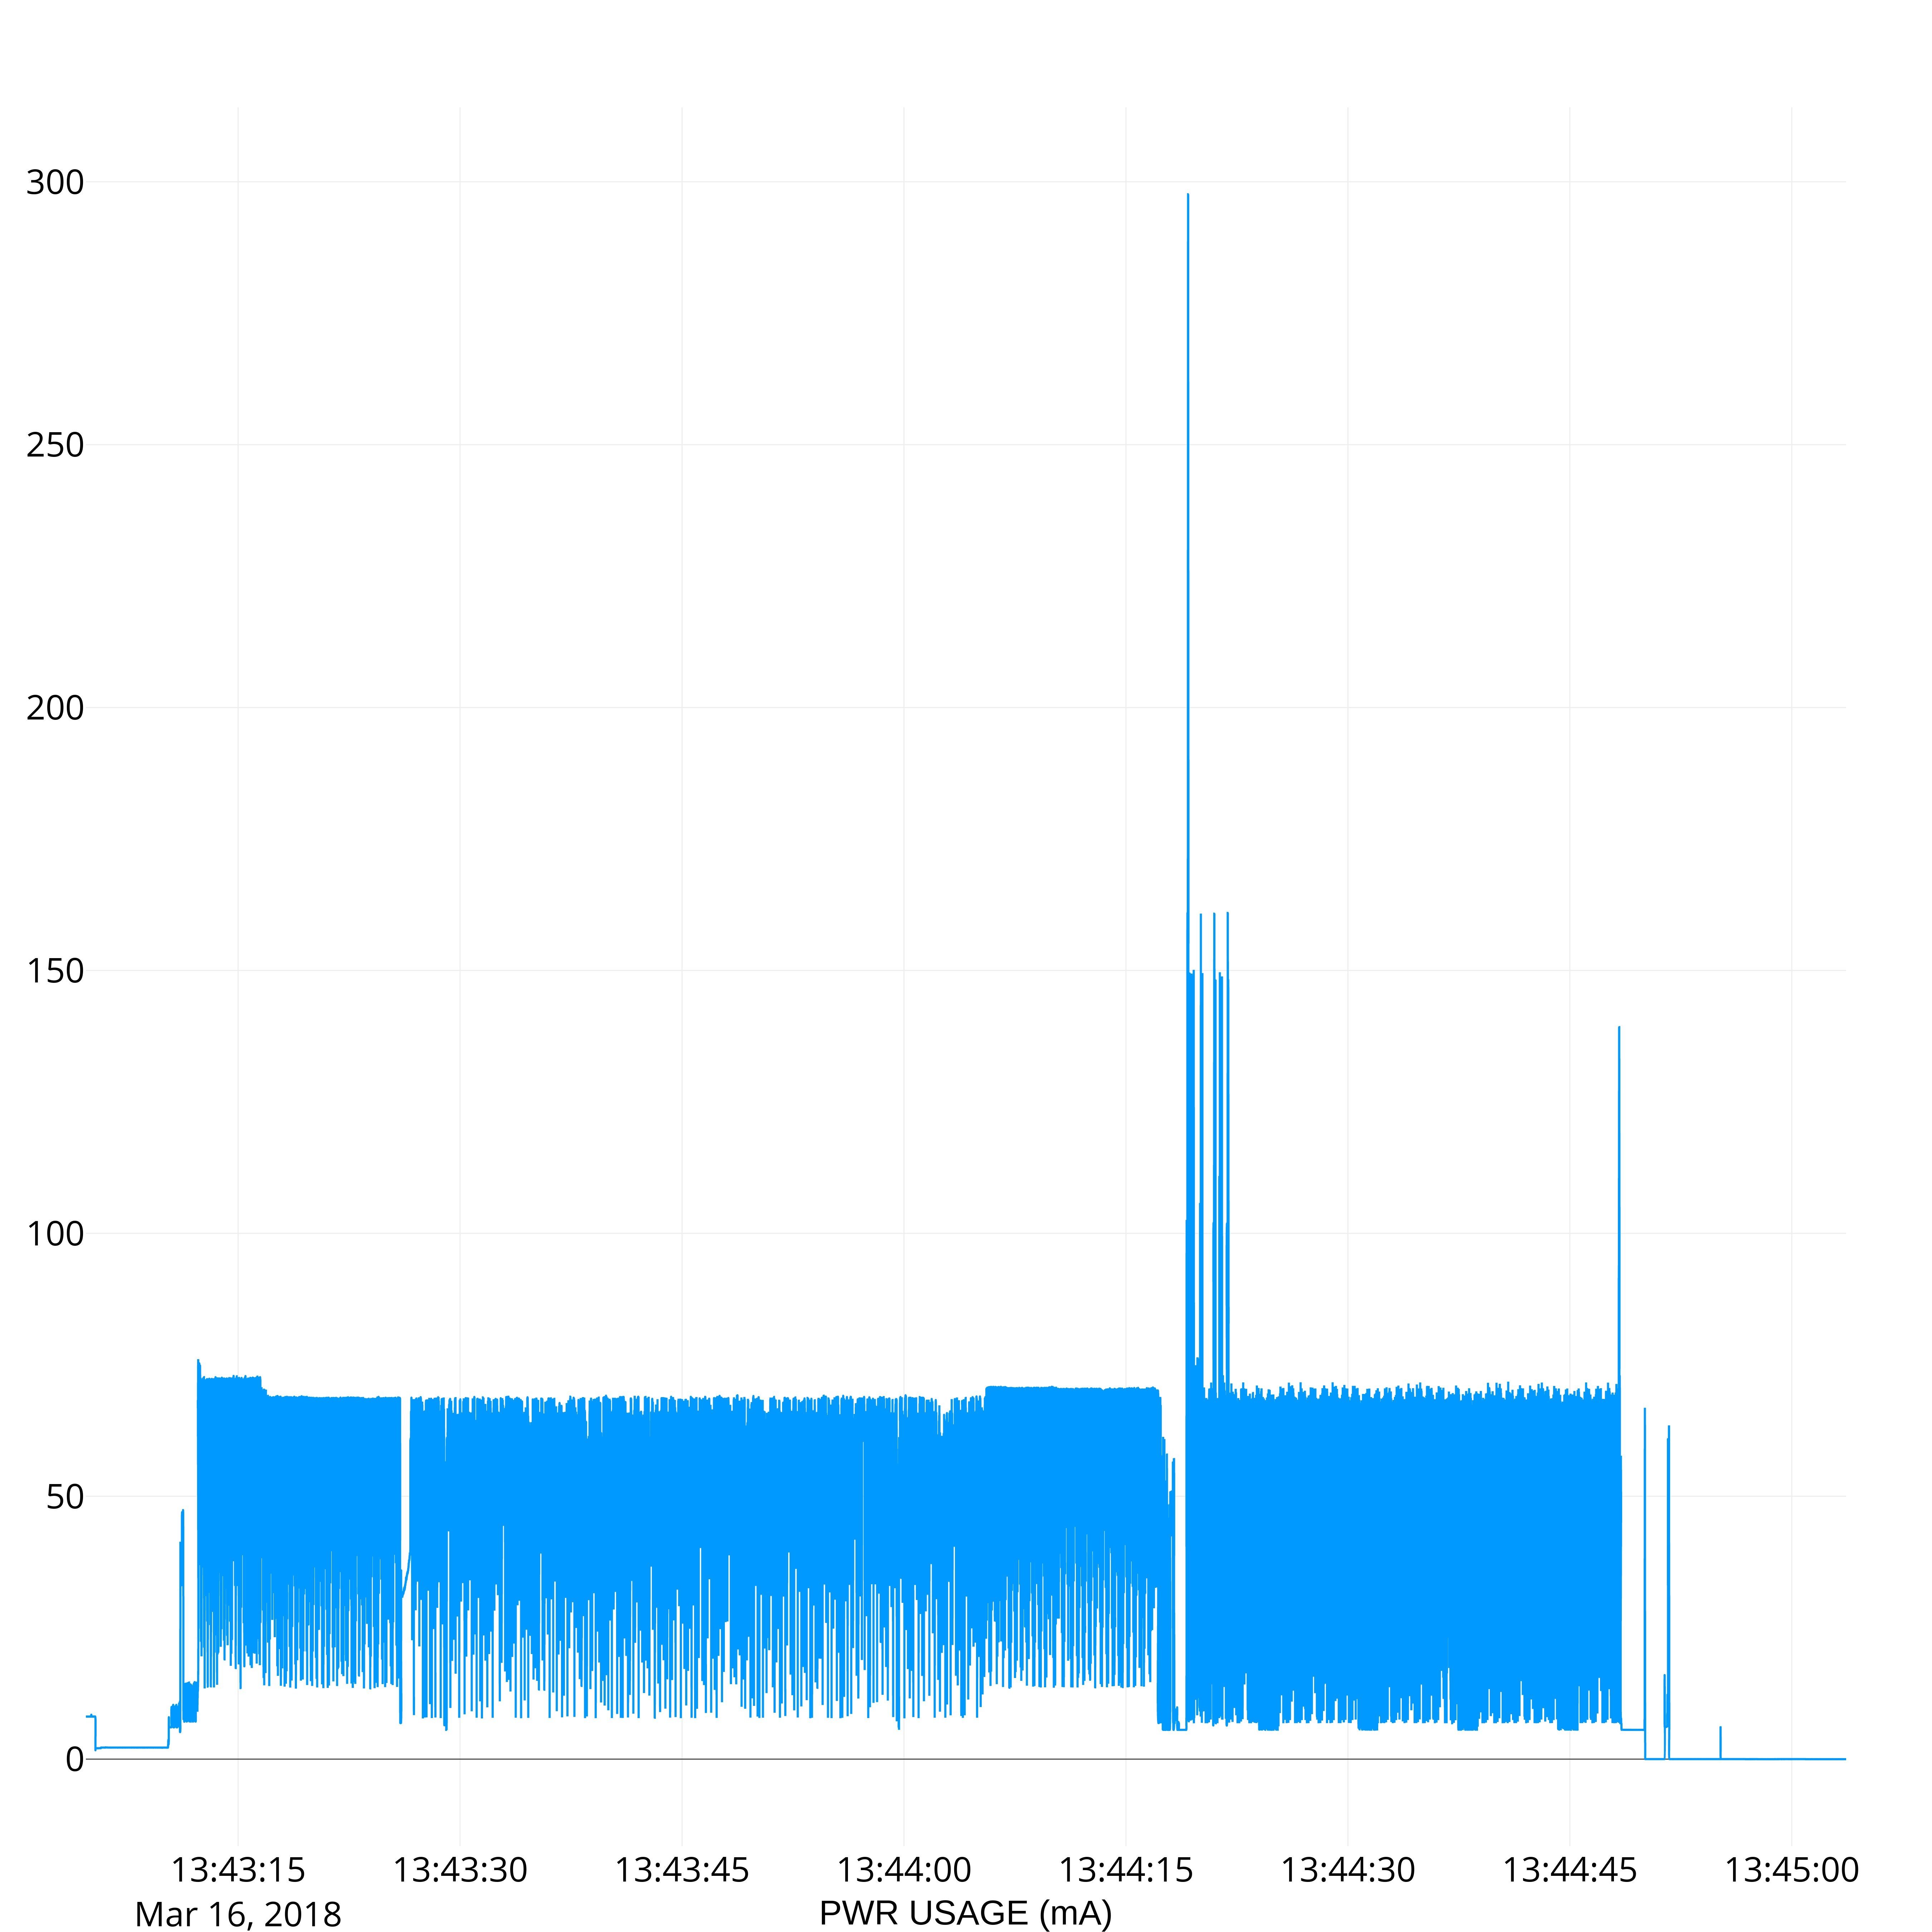
\includegraphics[width=0.9\textwidth, height=0.4\textheight]{/Users/henninghakonsen/Dropbox/Masteroppgave/thesis/latex/images/short_UiO_TELENOR_5_02_precision_reboot_2018-03-16_0_0x0_120_1_0.jpeg}
  \caption{Telenor reboot. Visit, \href{http://158.39.77.97:9000/\#/results/UiO\_TELENOR\_5.02\_precision\_reboot\_2018-03-16\_0\_0x0\_120\_1\_0}{webapp} \cite{online:result9}, for more details.}
  \label{figure:telenor_reboot}
\end{figure}

\begin{figure}[H]
  \centering
  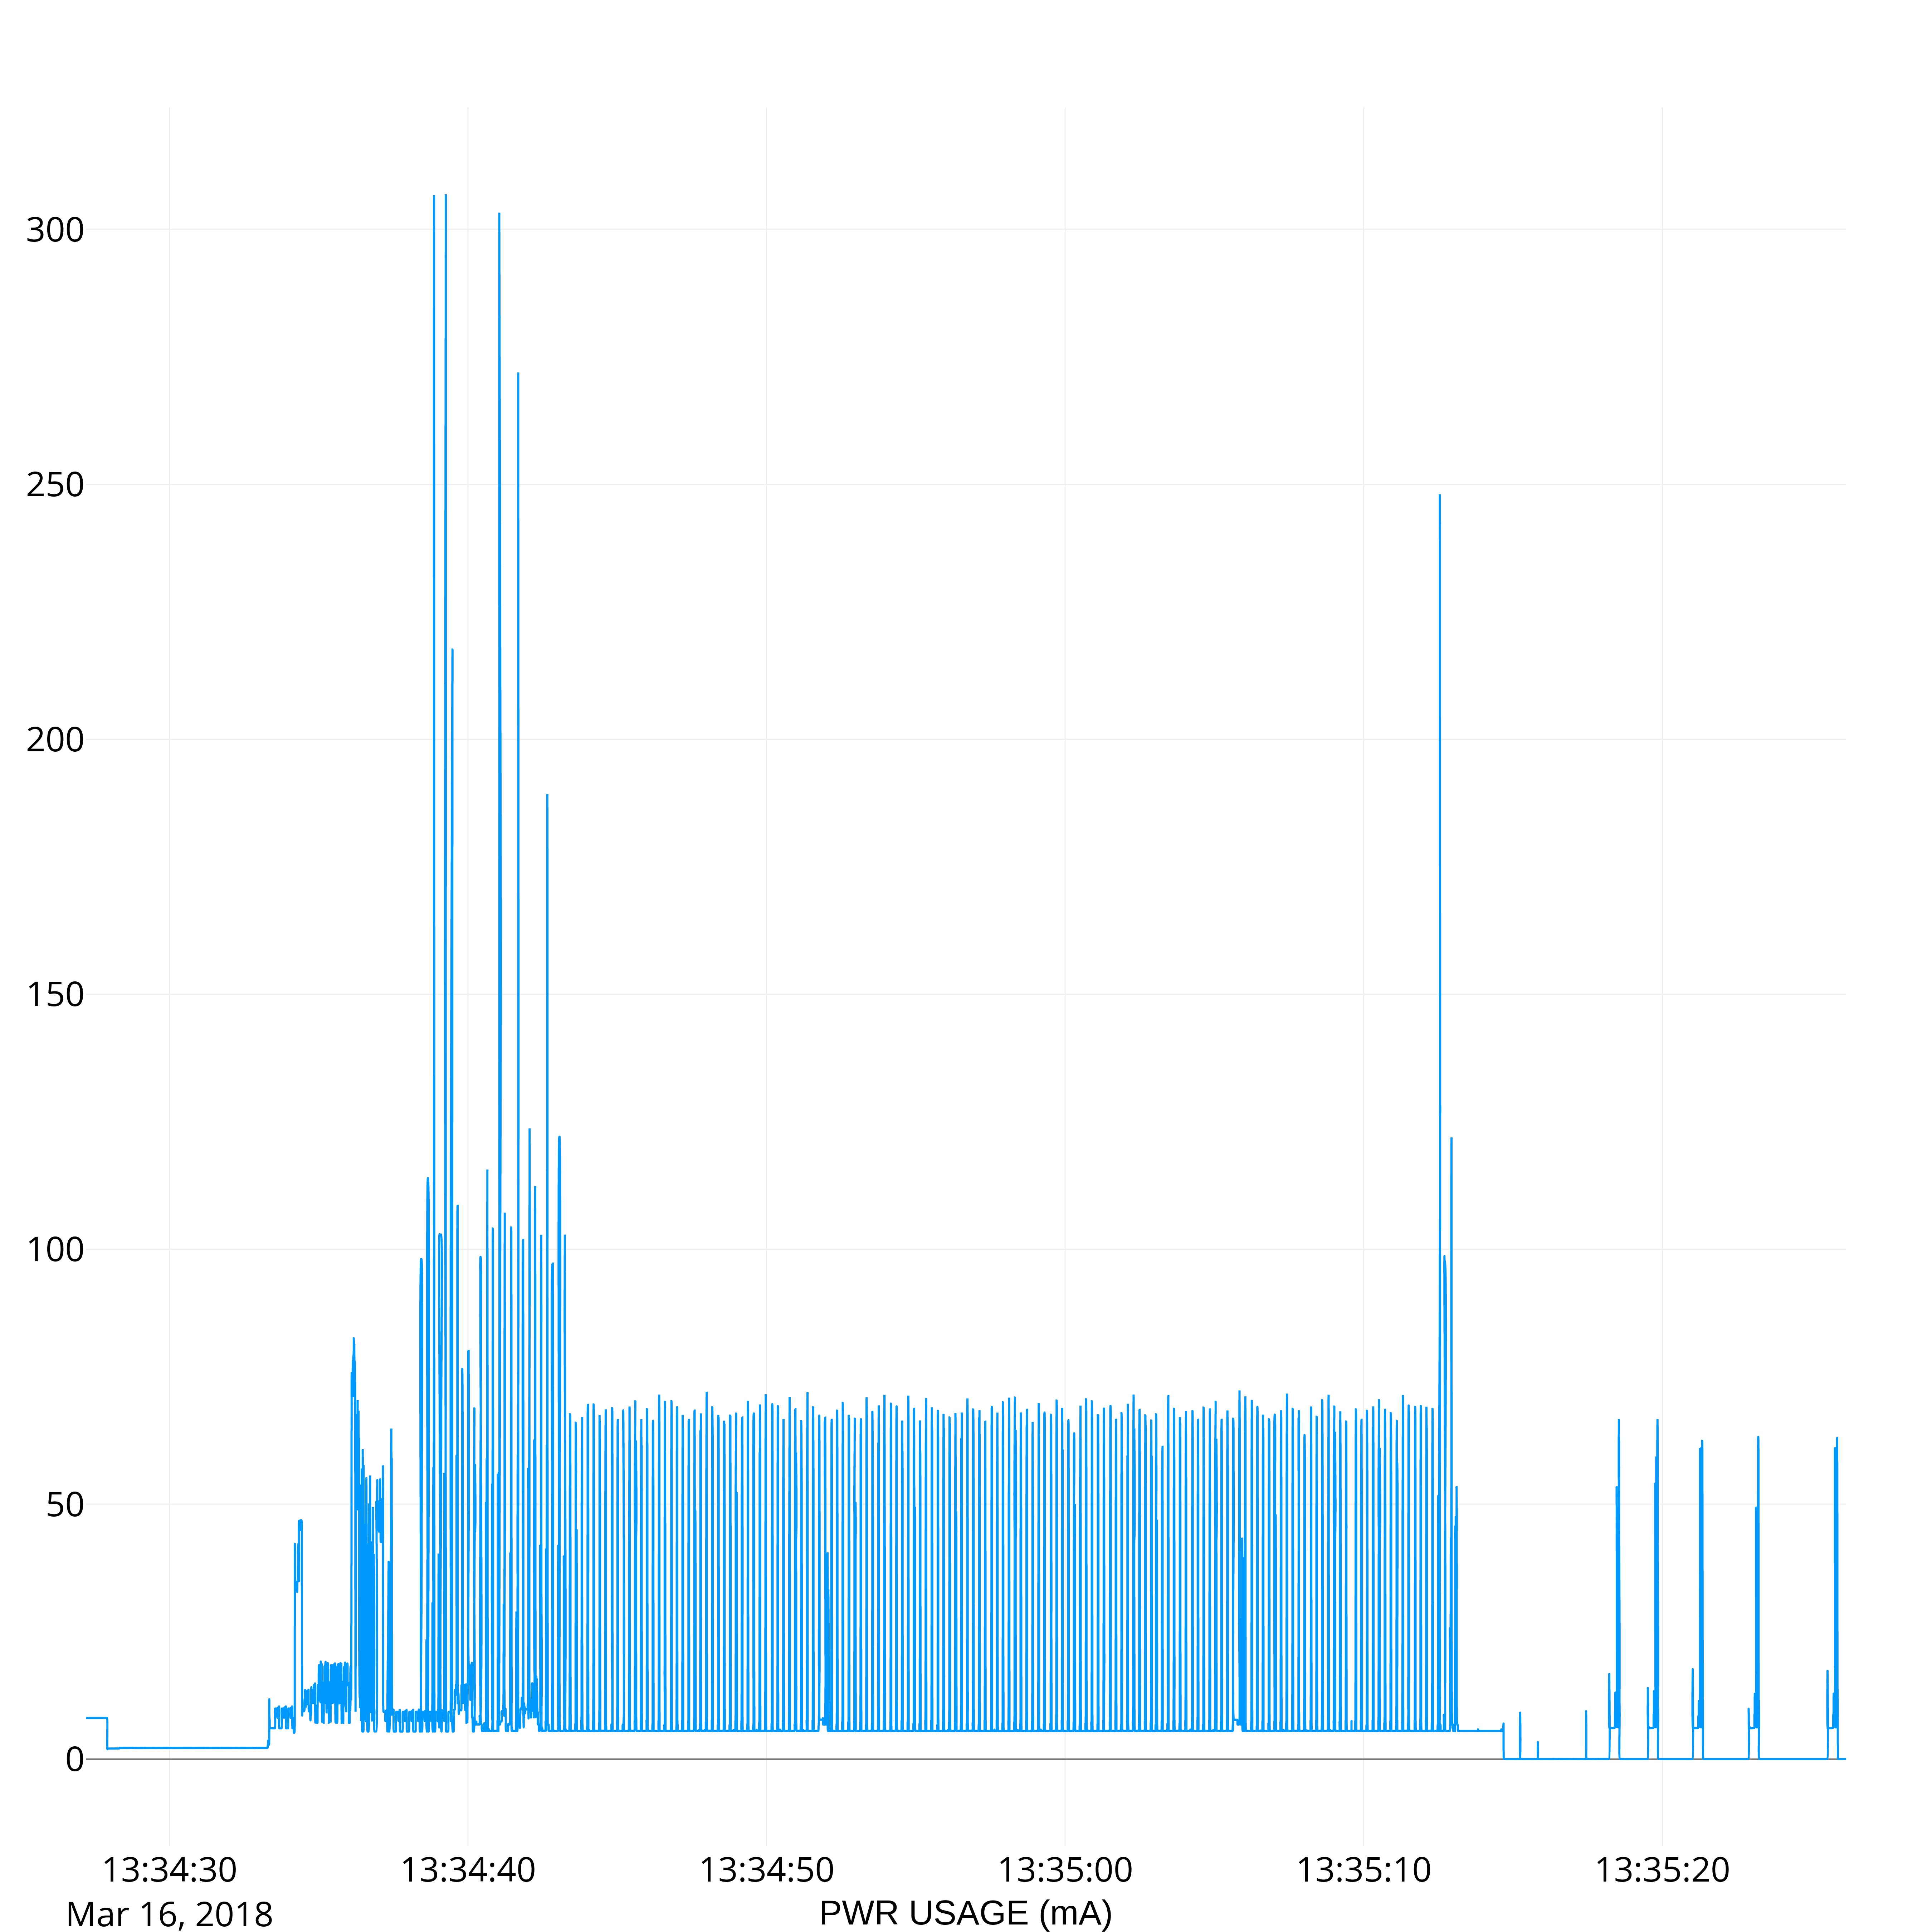
\includegraphics[width=0.9\textwidth, height=0.4\textheight]{/Users/henninghakonsen/Dropbox/Masteroppgave/thesis/latex/images/short_UiO_TELIA_5_02_precision_reboot_2018-03-16_0_0x0_60_1_0.jpeg}
  \caption{Telia reboot. Visit, \href{http://158.39.77.97:9000/\#/results/UiO\_TELIA\_5.02\_precision\_reboot\_2018-03-16\_0\_0x0\_60\_1\_0}{webapp} \cite{online:result10}, for more details.}
  \label{figure:telia_reboot}
\end{figure}

\subsection{Downtime test} \label{ssection:downtimetest}
If the network is down because of a power outage or similar breakdowns the \acrshort{ue} might be disconnected from the network if there are no other \acrshort{enb}'s in the close proximity. We had a period where the device actually lost connection to the network, even though the signal strength showed otherwise. In figure, \vref{figure:downtime}, you can see a longer monitoring sequence. At first the device transmits data, but after a short while it is disconnected and the subsequent results gives us an indication of what happens if the device looses connection. We see that the receive/transmit timers does not change, hence we believe that the device does not use any effort trying to reconnect to the network. We will discuss different approaches to this problem in section, \vref{section:guidelines}.

\begin{figure}[H]
  \centering
  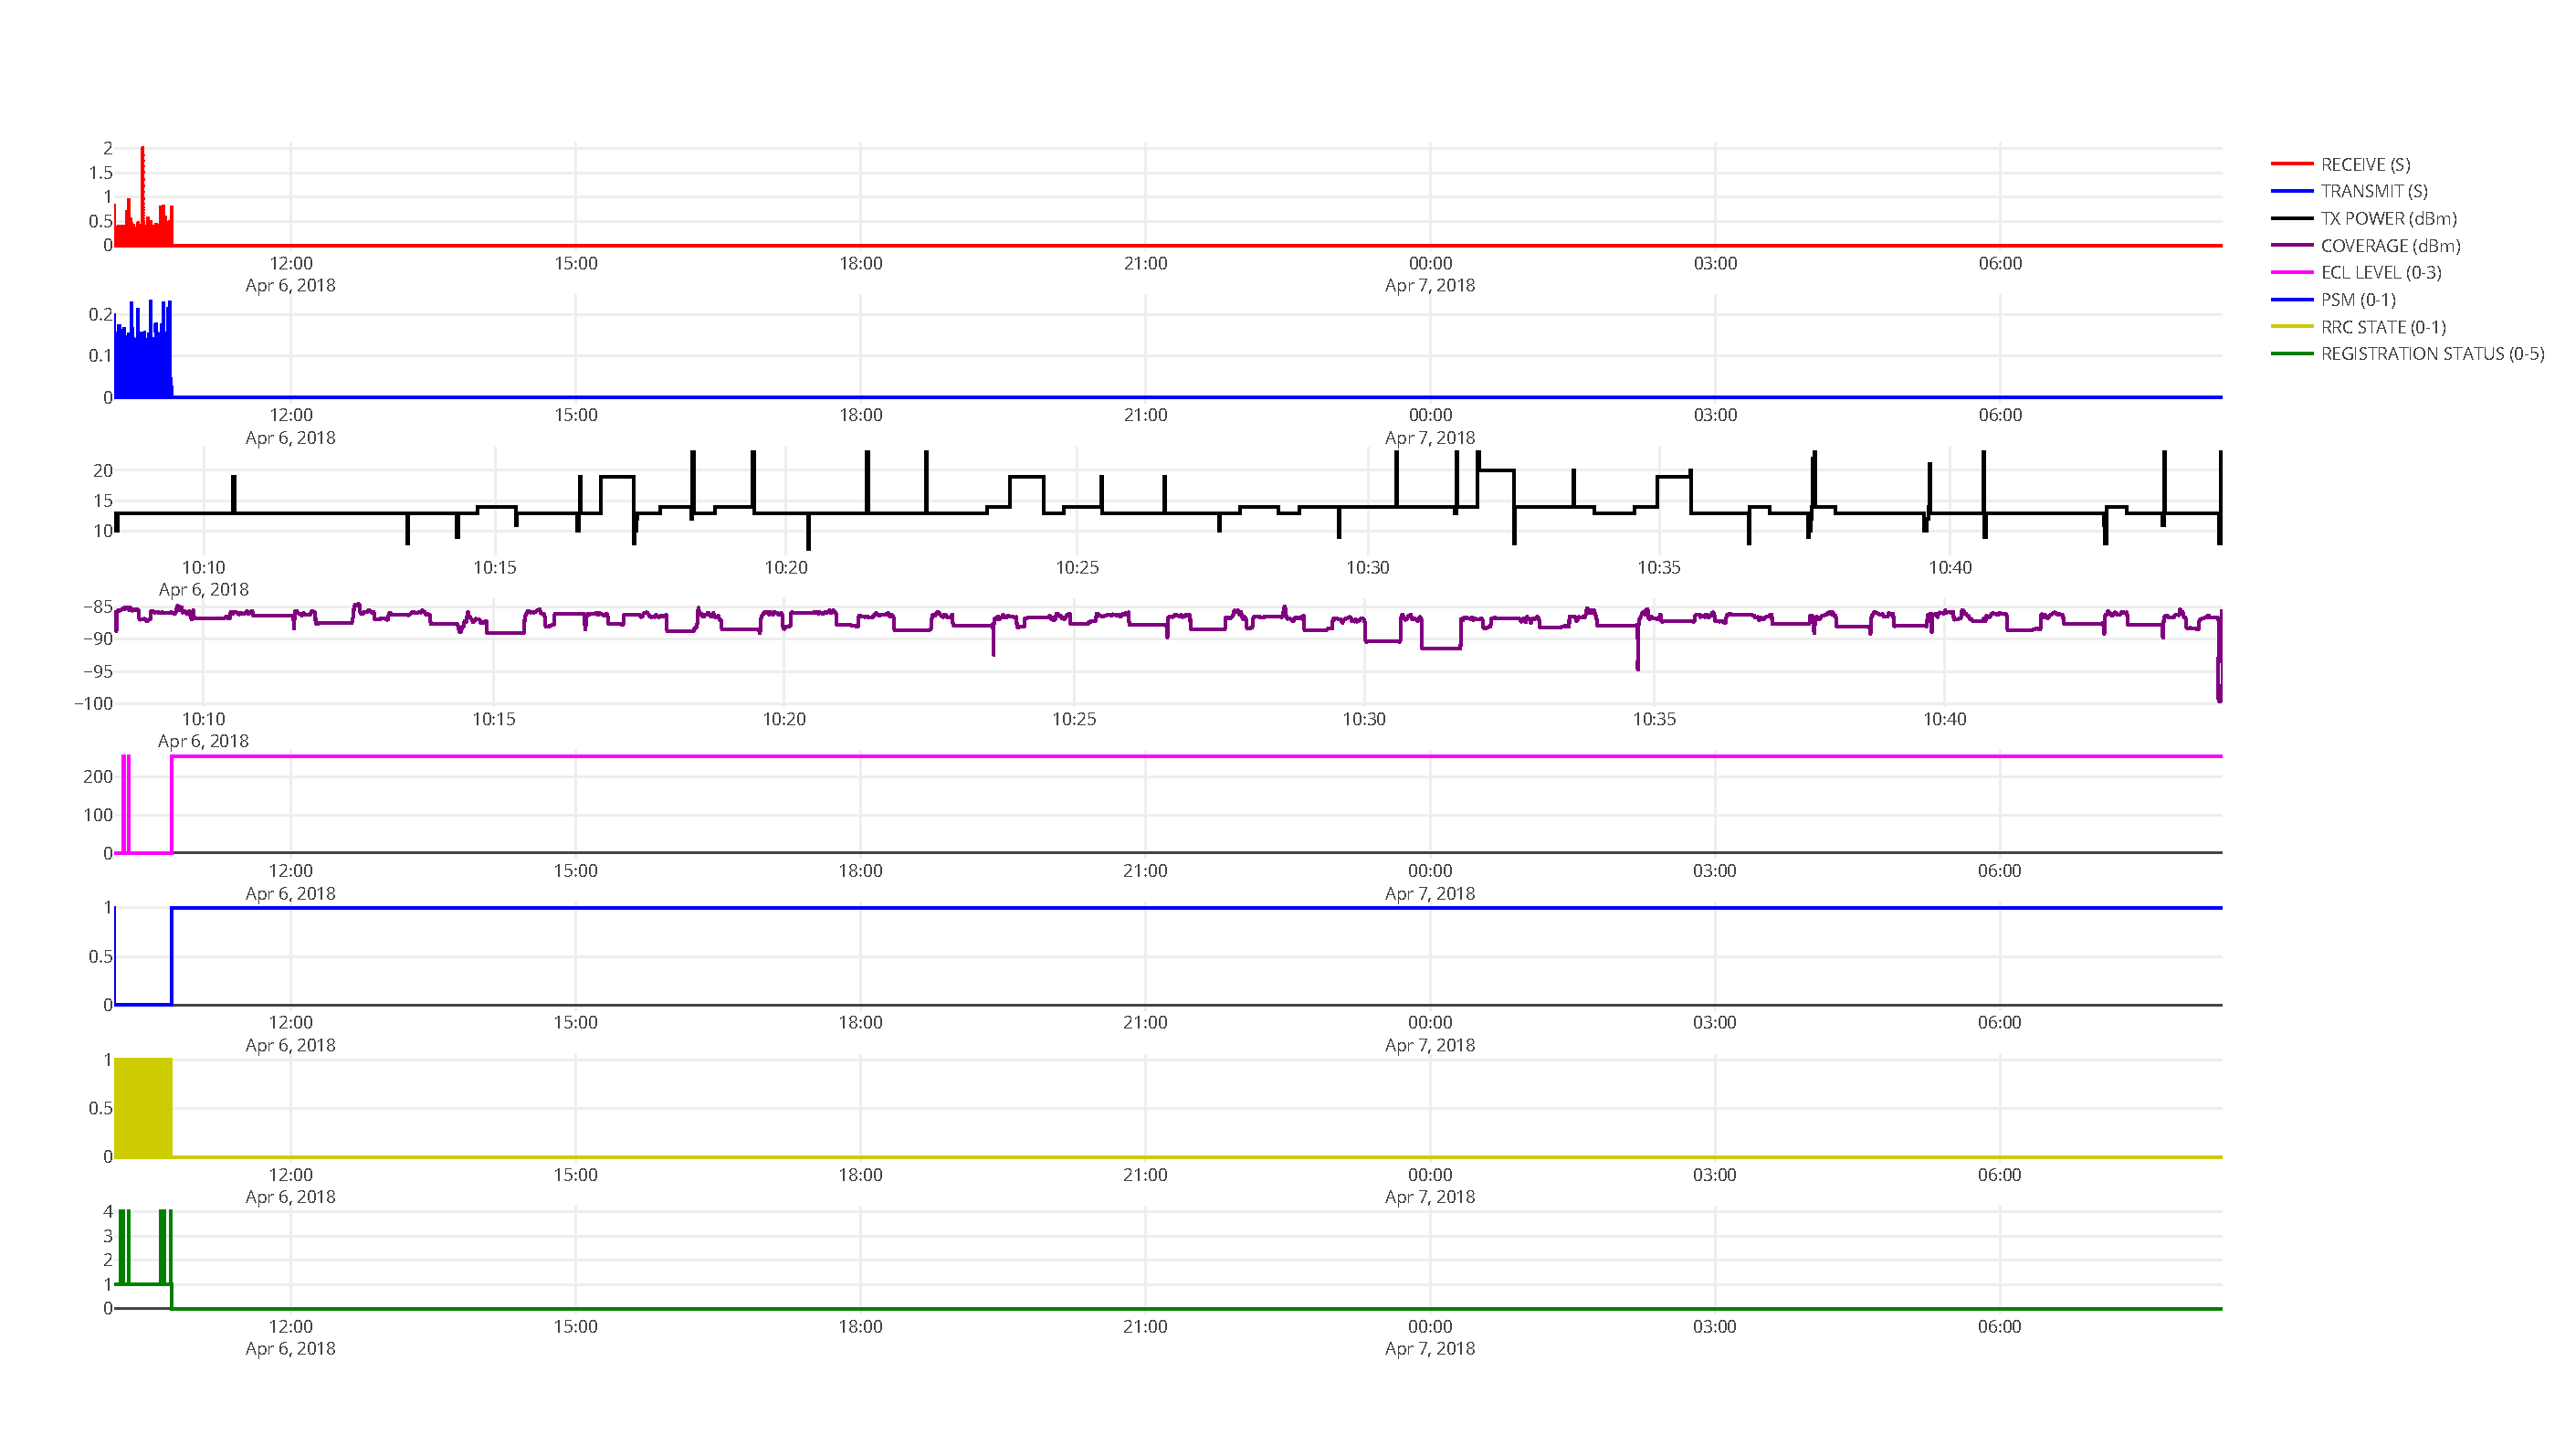
\includegraphics[width=0.9\textwidth, height=0.4\textheight]{/Users/henninghakonsen/Dropbox/Masteroppgave/thesis/latex/images/downtime.pdf}
  \caption{Example of disconnection from the network}
  \label{figure:downtime}
\end{figure}

\cleardoublepage
\section{Short term figures}
\subsection{General} \label{ssection:general}
\begin{figure}[H]
  \centering
  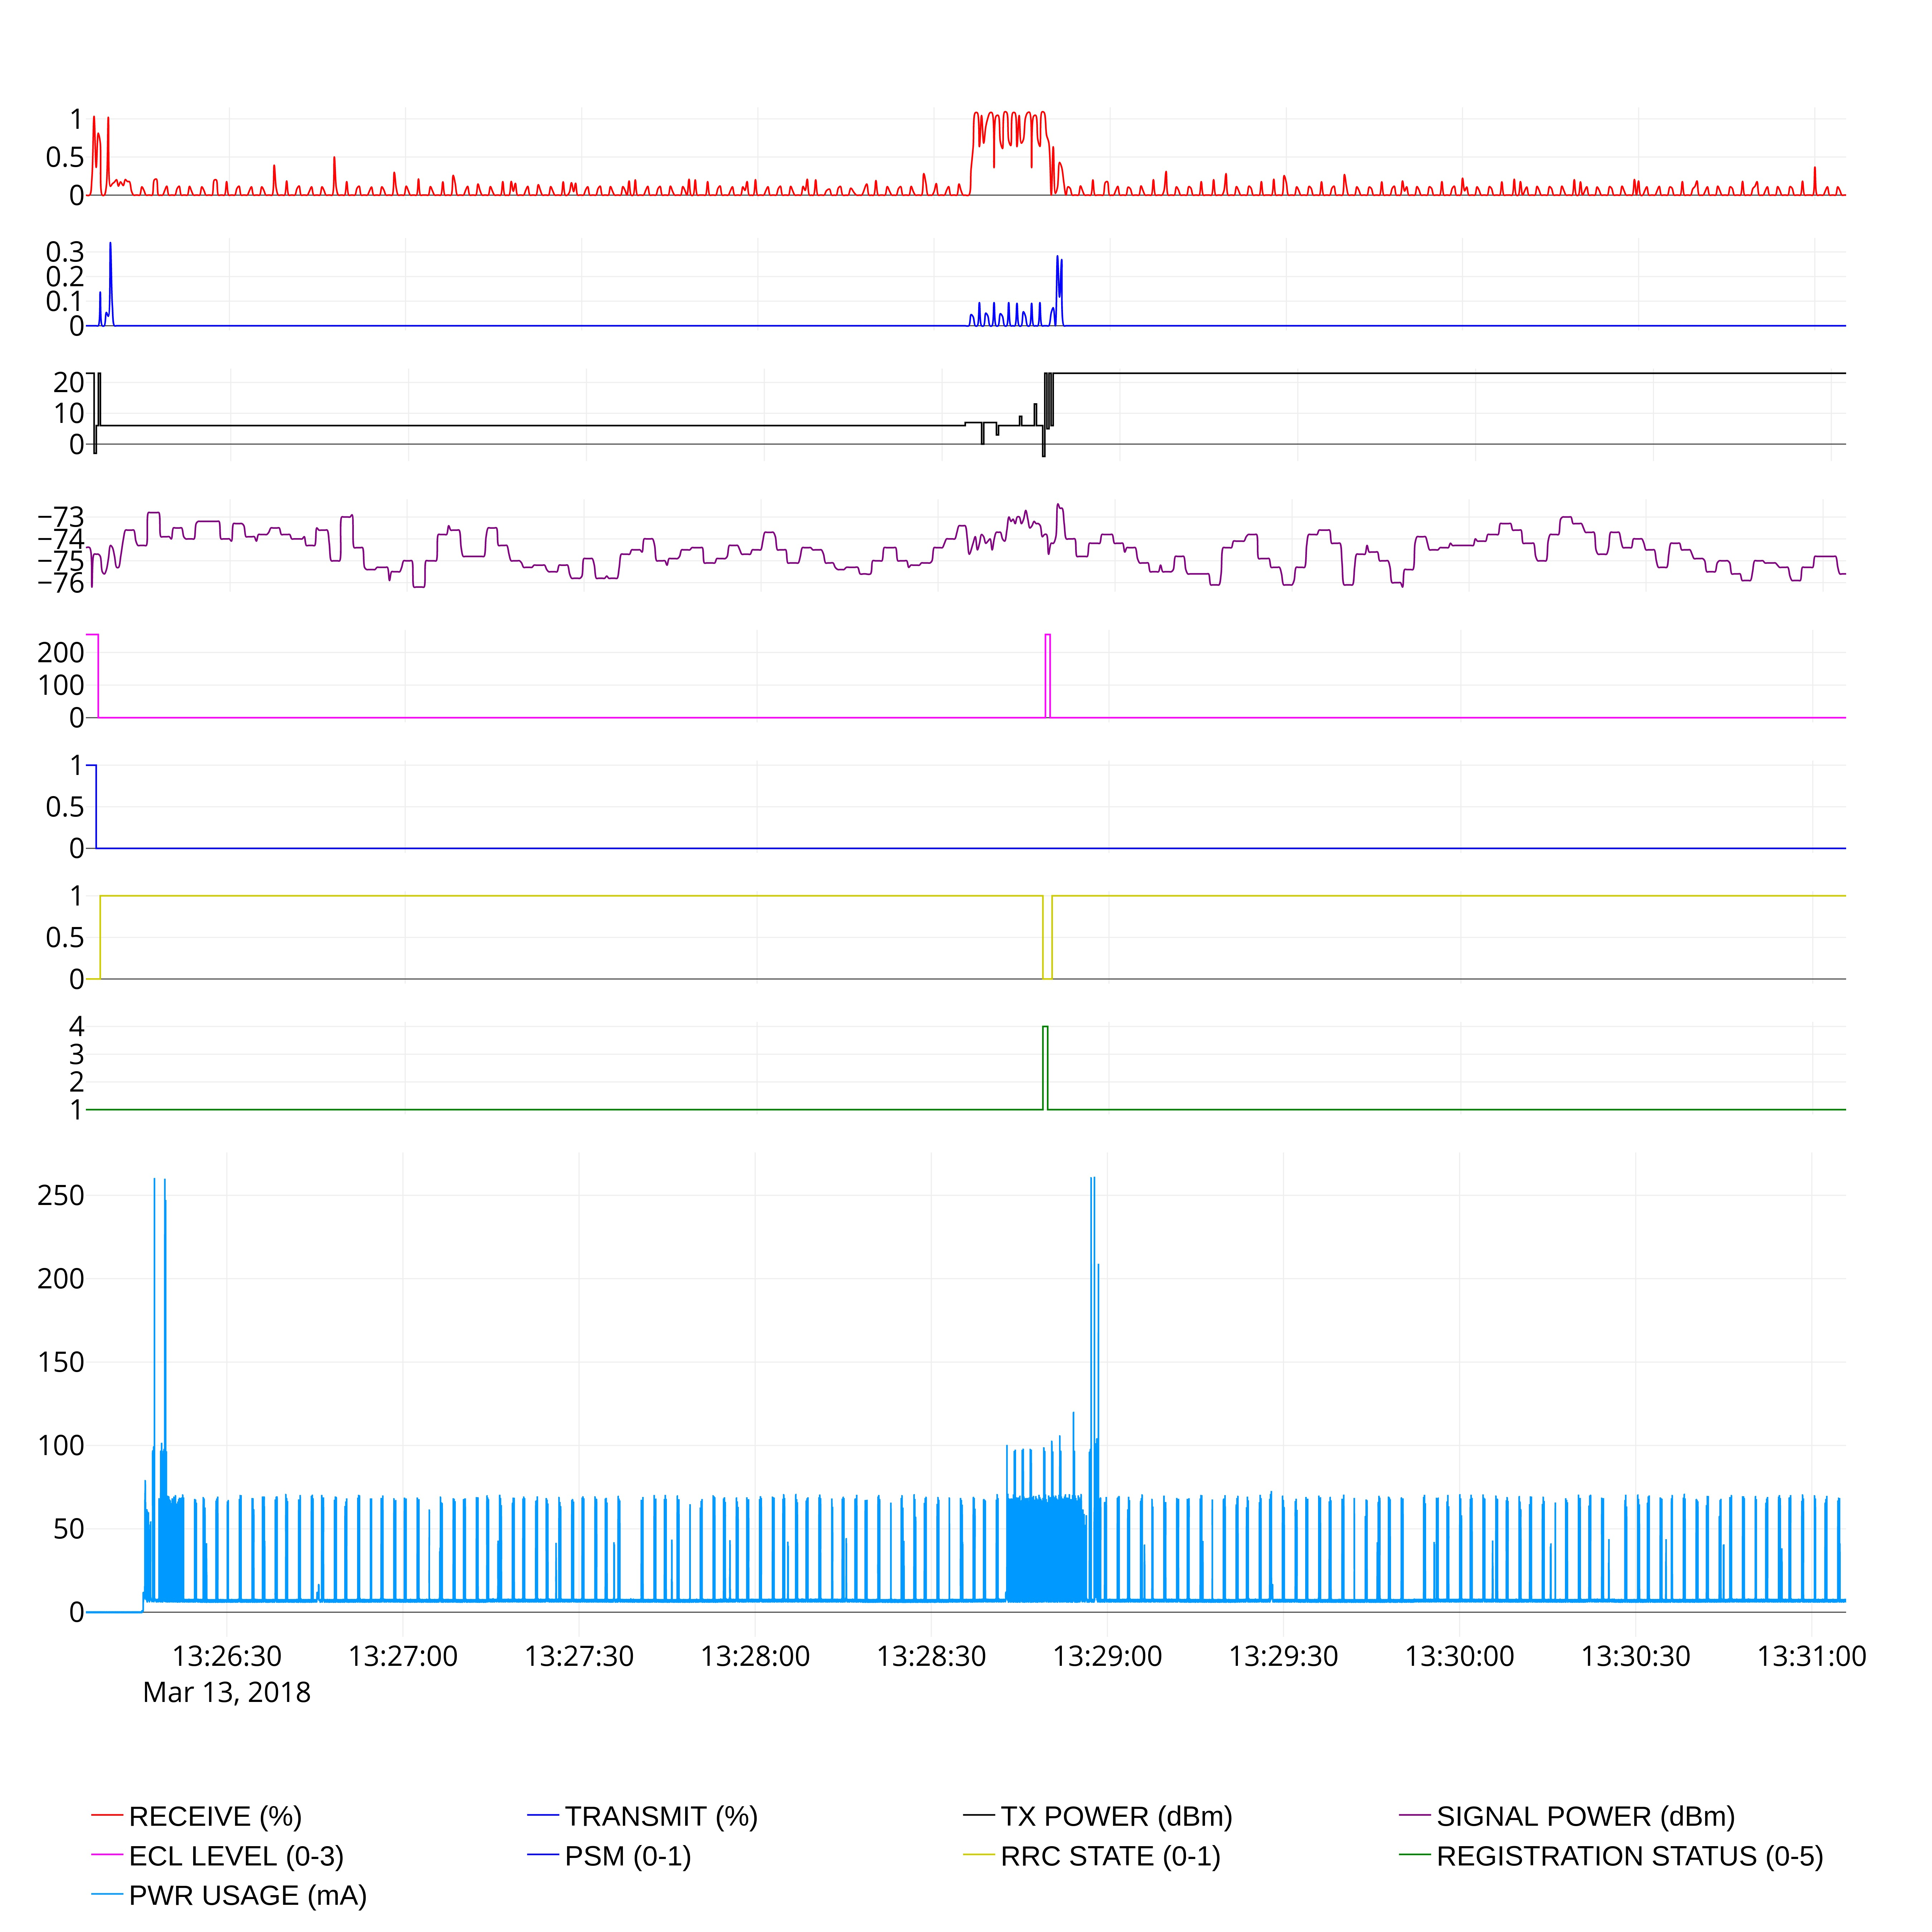
\includegraphics[width=0.9\textwidth, height=0.8\textheight]{/Users/henninghakonsen/Dropbox/Masteroppgave/thesis/latex/images/full_Q-FREE_TELIA_5_02_precision_2018-03-13_1_0x0_150_2_100.jpeg}
  \caption{Weird behavior, 2 x 150, Telia.}
  \label{figure:2x150_QFREE_TELIA}
\end{figure}

\begin{figure}[H]
  \centering
  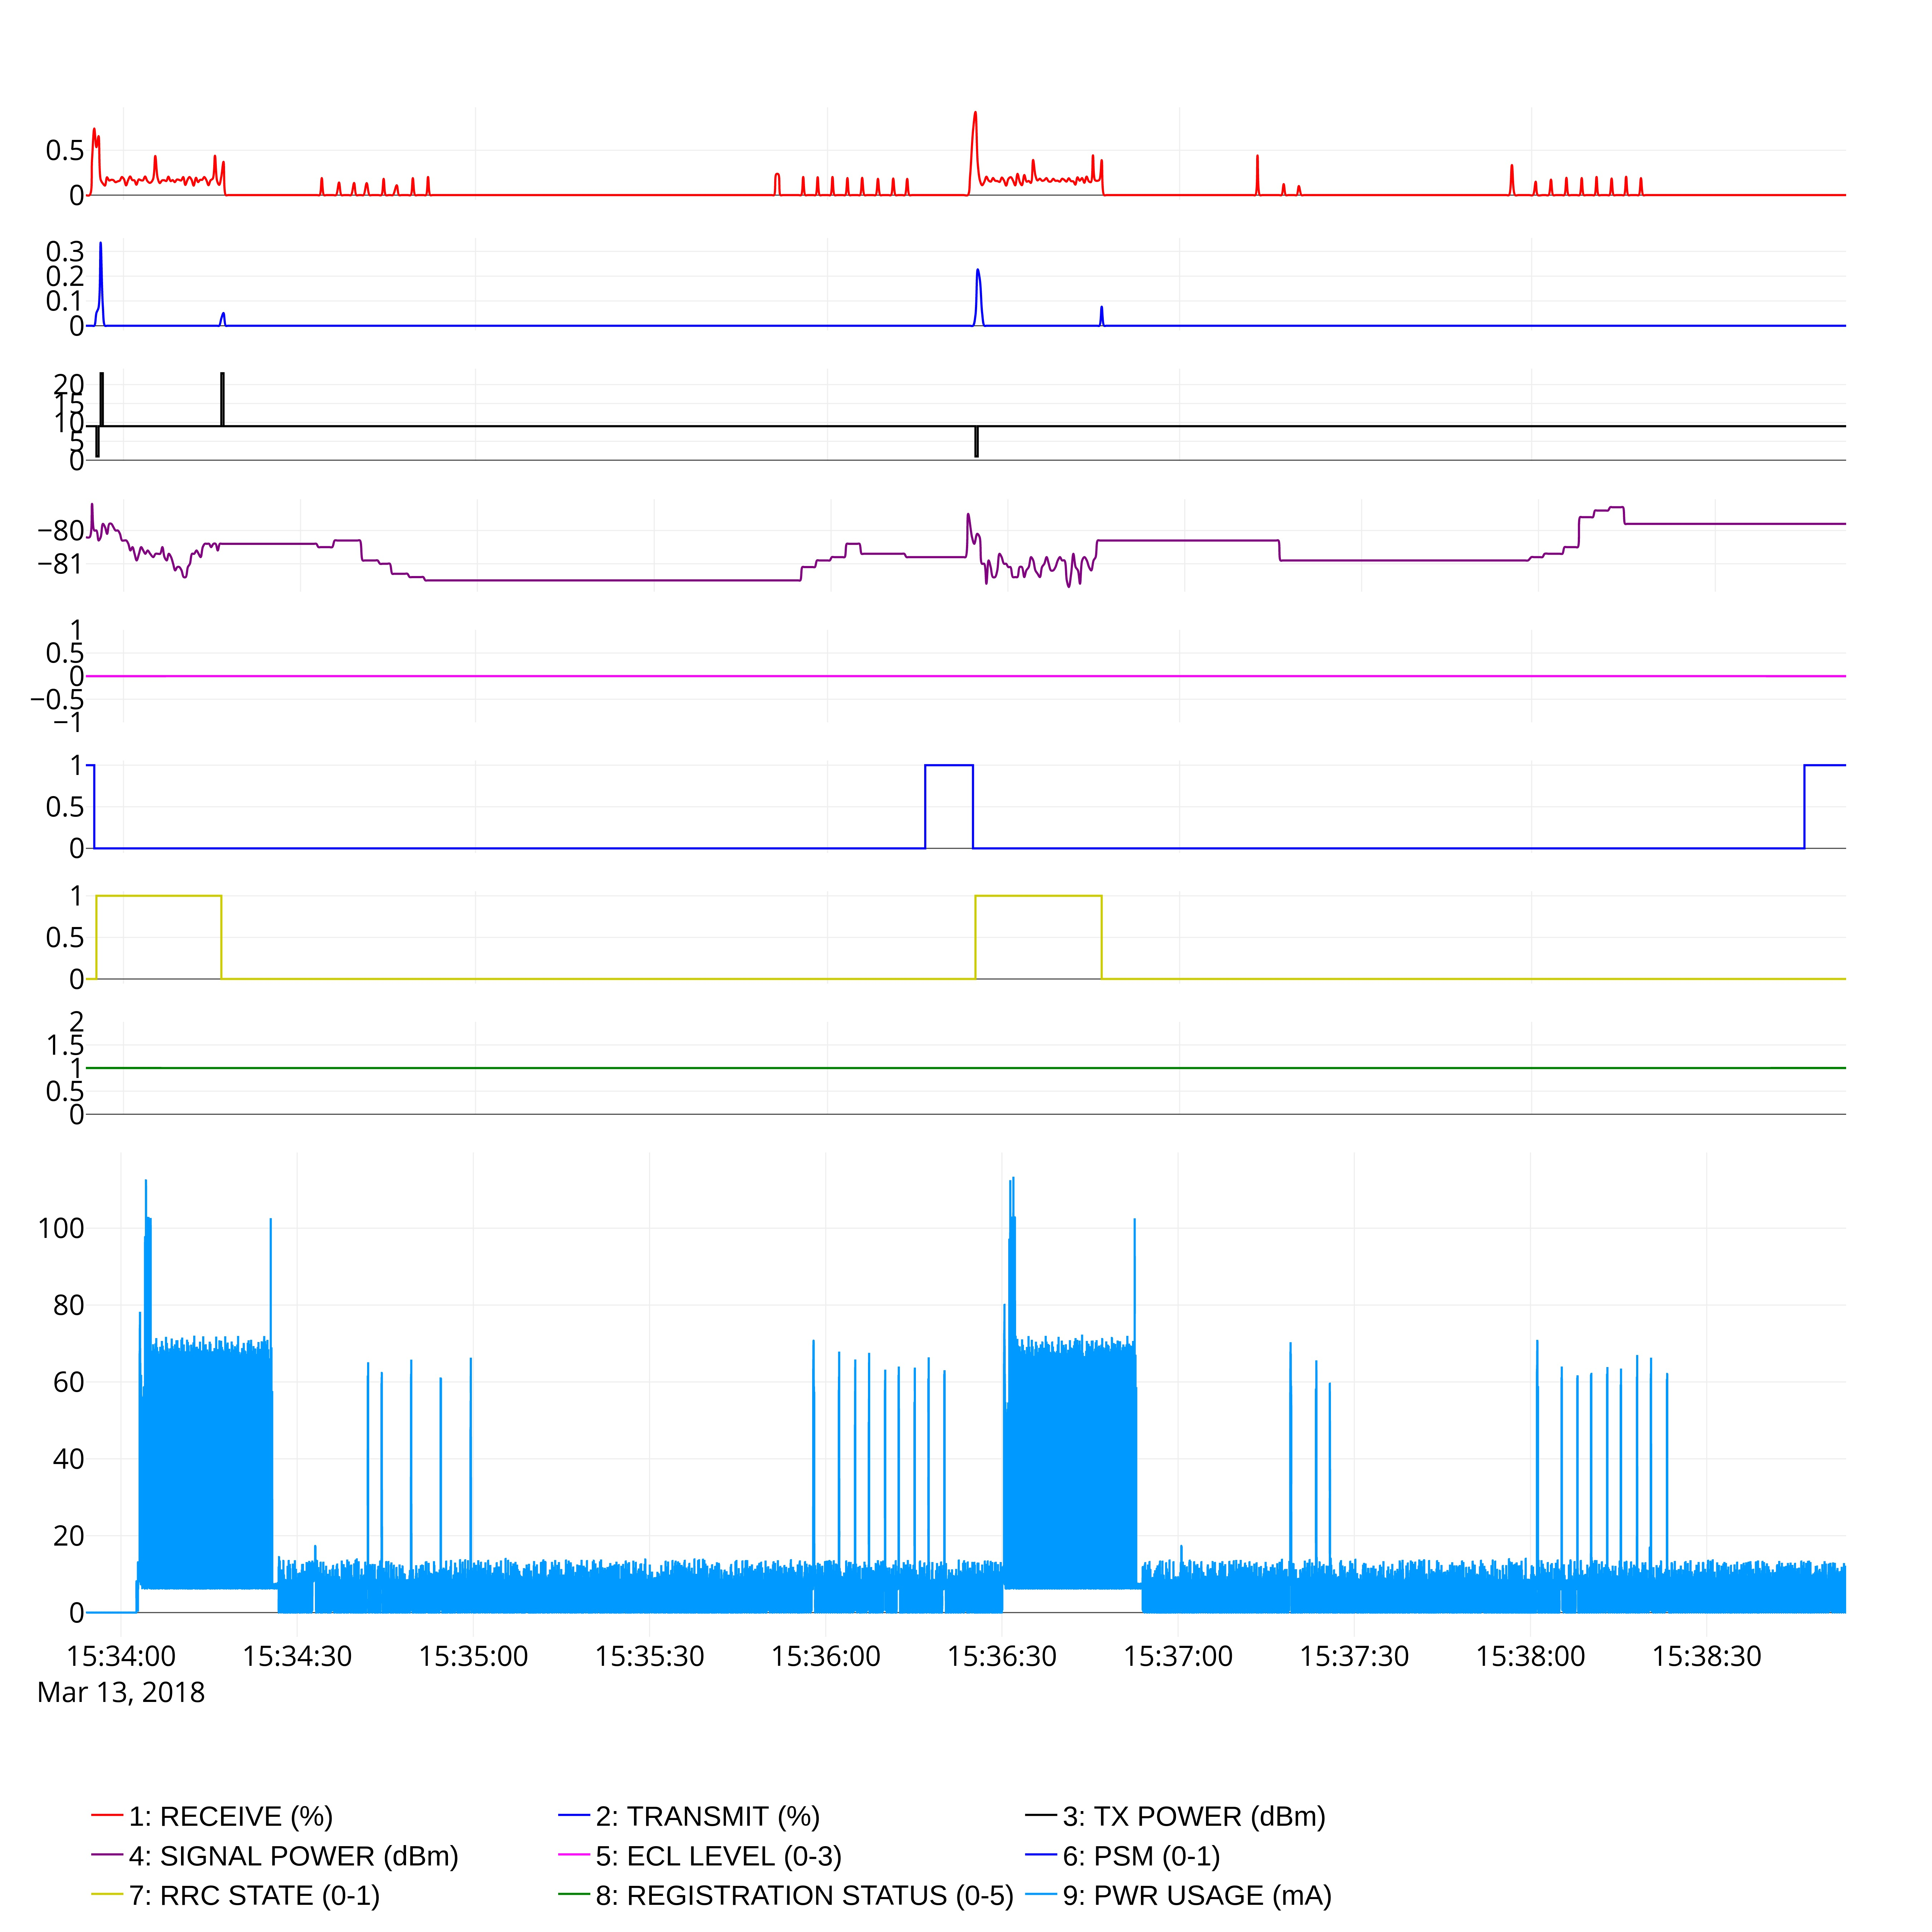
\includegraphics[width=0.9\textwidth, height=0.8\textheight]{/Users/henninghakonsen/Dropbox/Masteroppgave/thesis/latex/images/full_UiO_TELIA_5_02_precision_2018-03-13_1_0x0_150_2_100.jpeg}
  \caption{Normal behavior, 2 x 150 UiO, Telia.}
  \label{figure:2x150_UIO_TELIA}
\end{figure}

\begin{figure}[H]
  \centering
  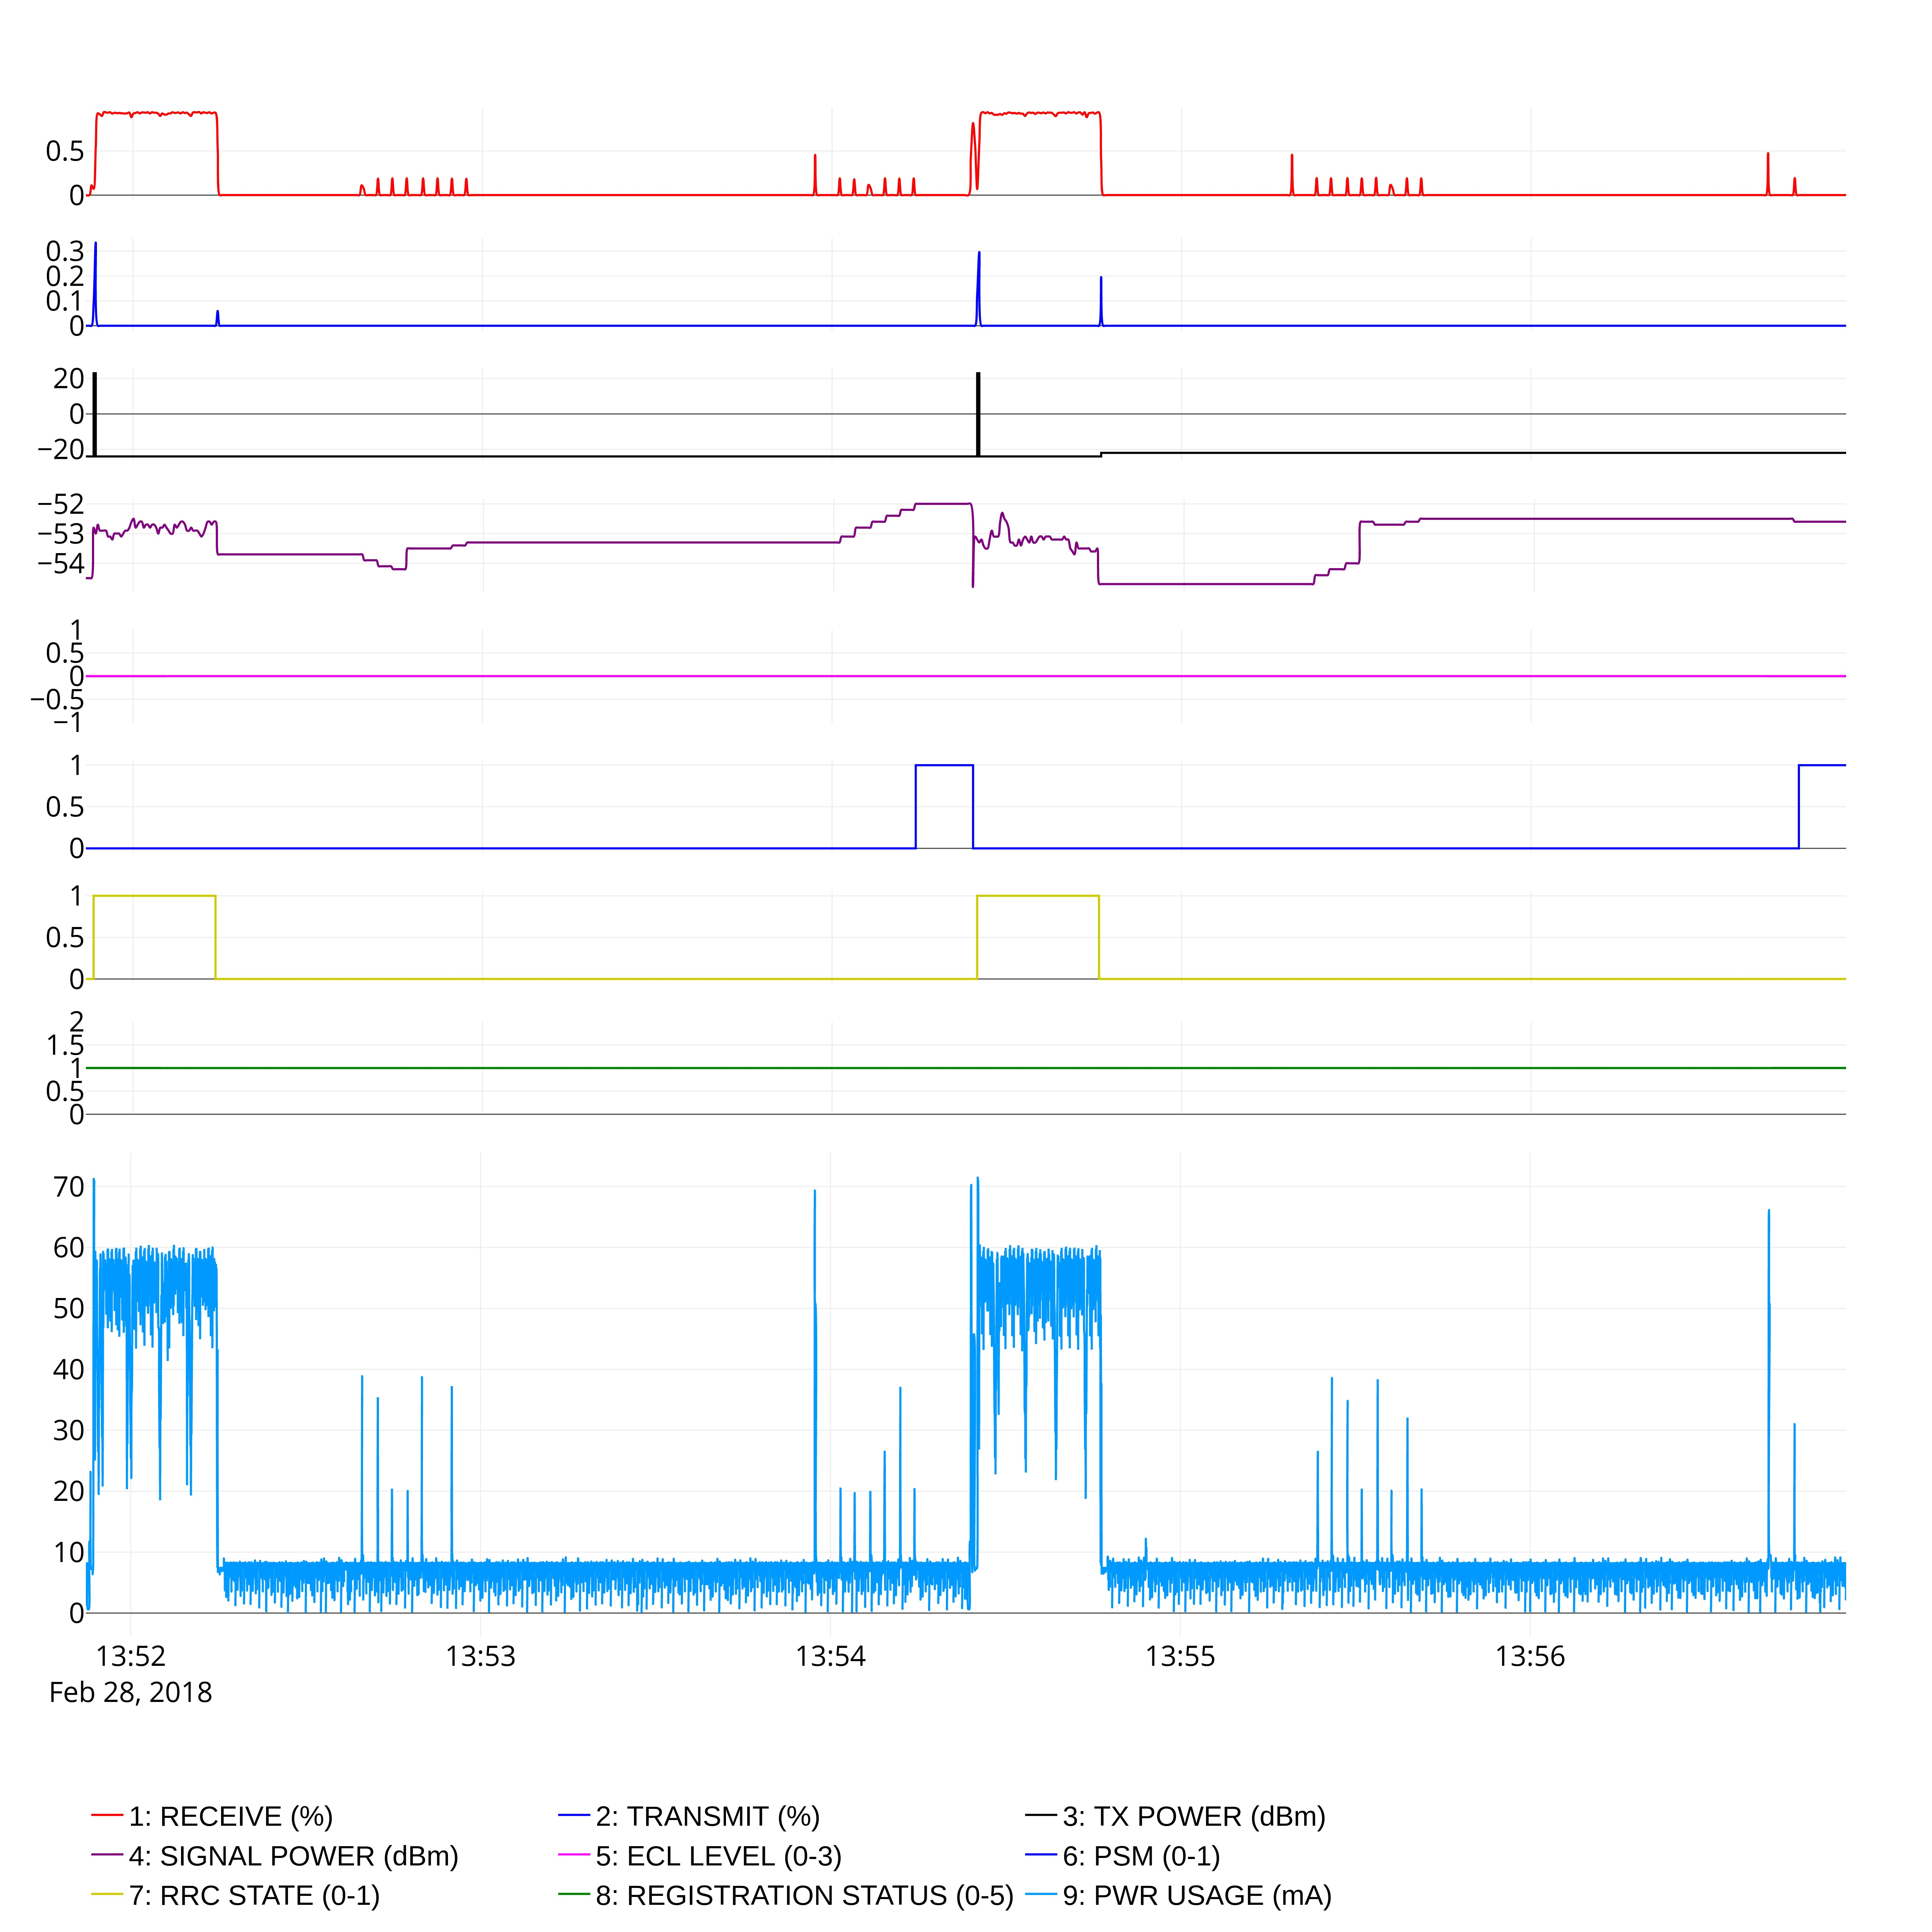
\includegraphics[width=0.9\textwidth, height=0.8\textheight]{/Users/henninghakonsen/Dropbox/Masteroppgave/thesis/latex/images/full_Q-FREE_TELENOR_2018-02-28_1_0x0_150_2_100.jpeg}
  \caption{Normal behavior, 2 x 150 Q-FREE, Telenor.}
  \label{figure:2x150_QFREE_TELENOR}
\end{figure}

\subsection{Downtime prior to transmit} \label{ssection:downtimeprior}
\begin{figure}[H]
  \centering
  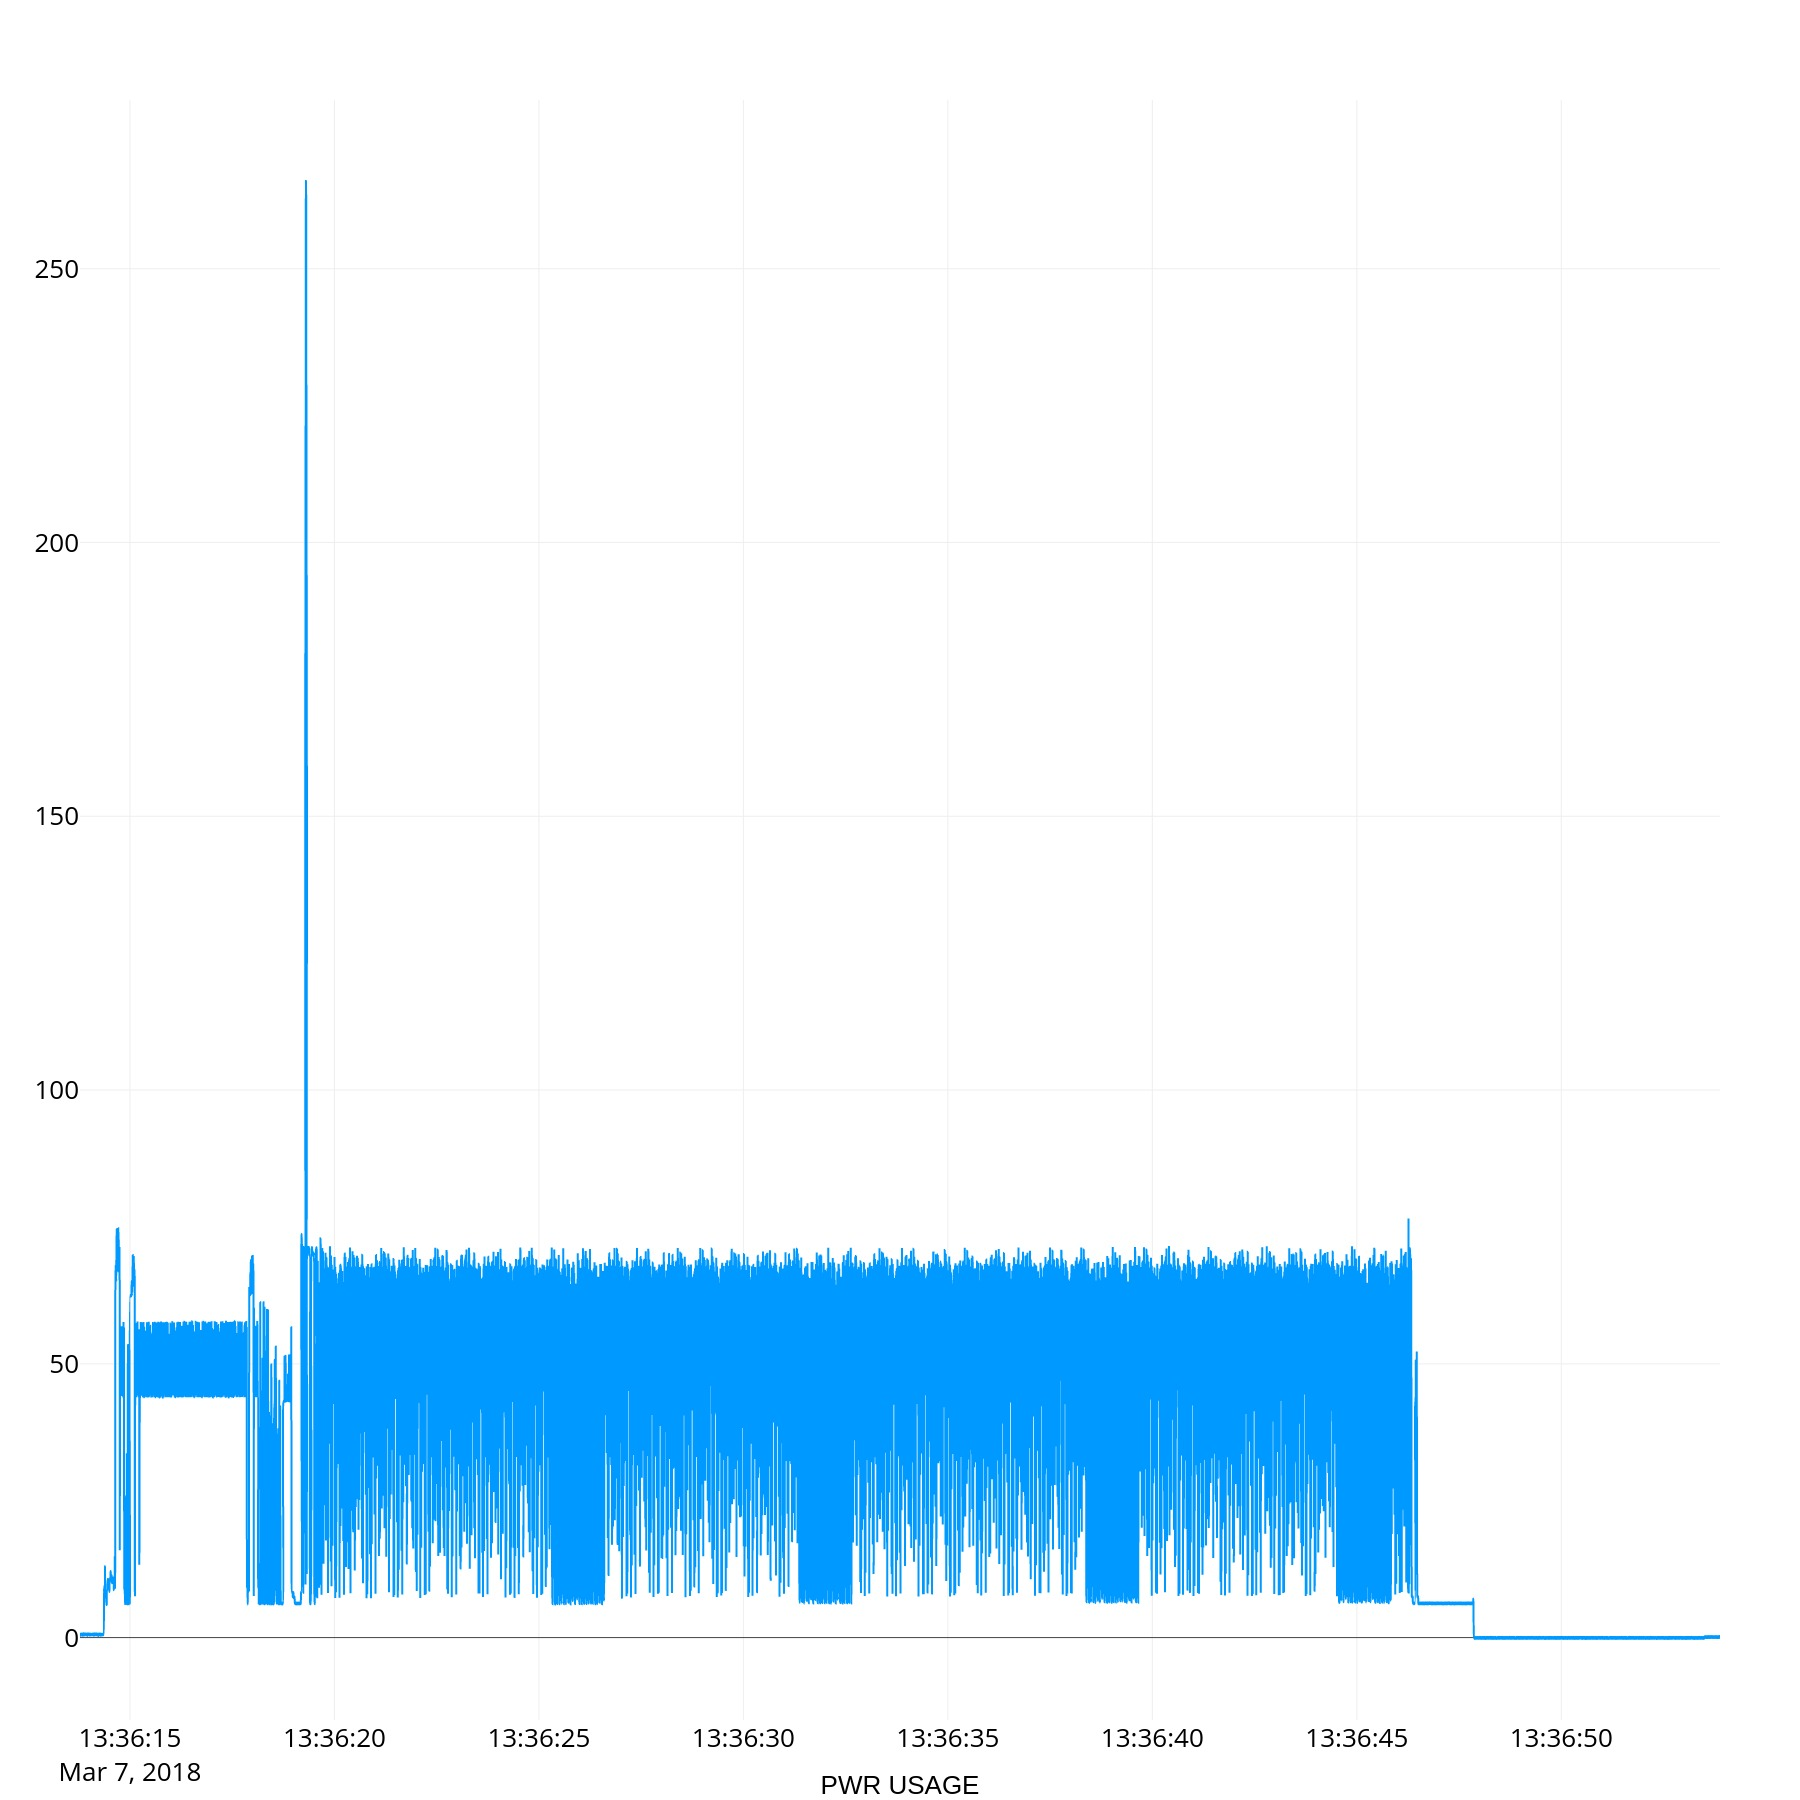
\includegraphics[width=0.9\textwidth, height=0.8\textheight]{/Users/henninghakonsen/Dropbox/Masteroppgave/thesis/latex/images/short_Q-FREE_TELENOR_5_02_2018-03-07_0_0x0_40_1_200.jpeg}
  \caption{1 x 40 Q-FREE, Telenor - no device logging.}
  \label{figure:1x40_QFREE_TELENOR_0LOG}
\end{figure}

\begin{figure}[H]
  \centering
  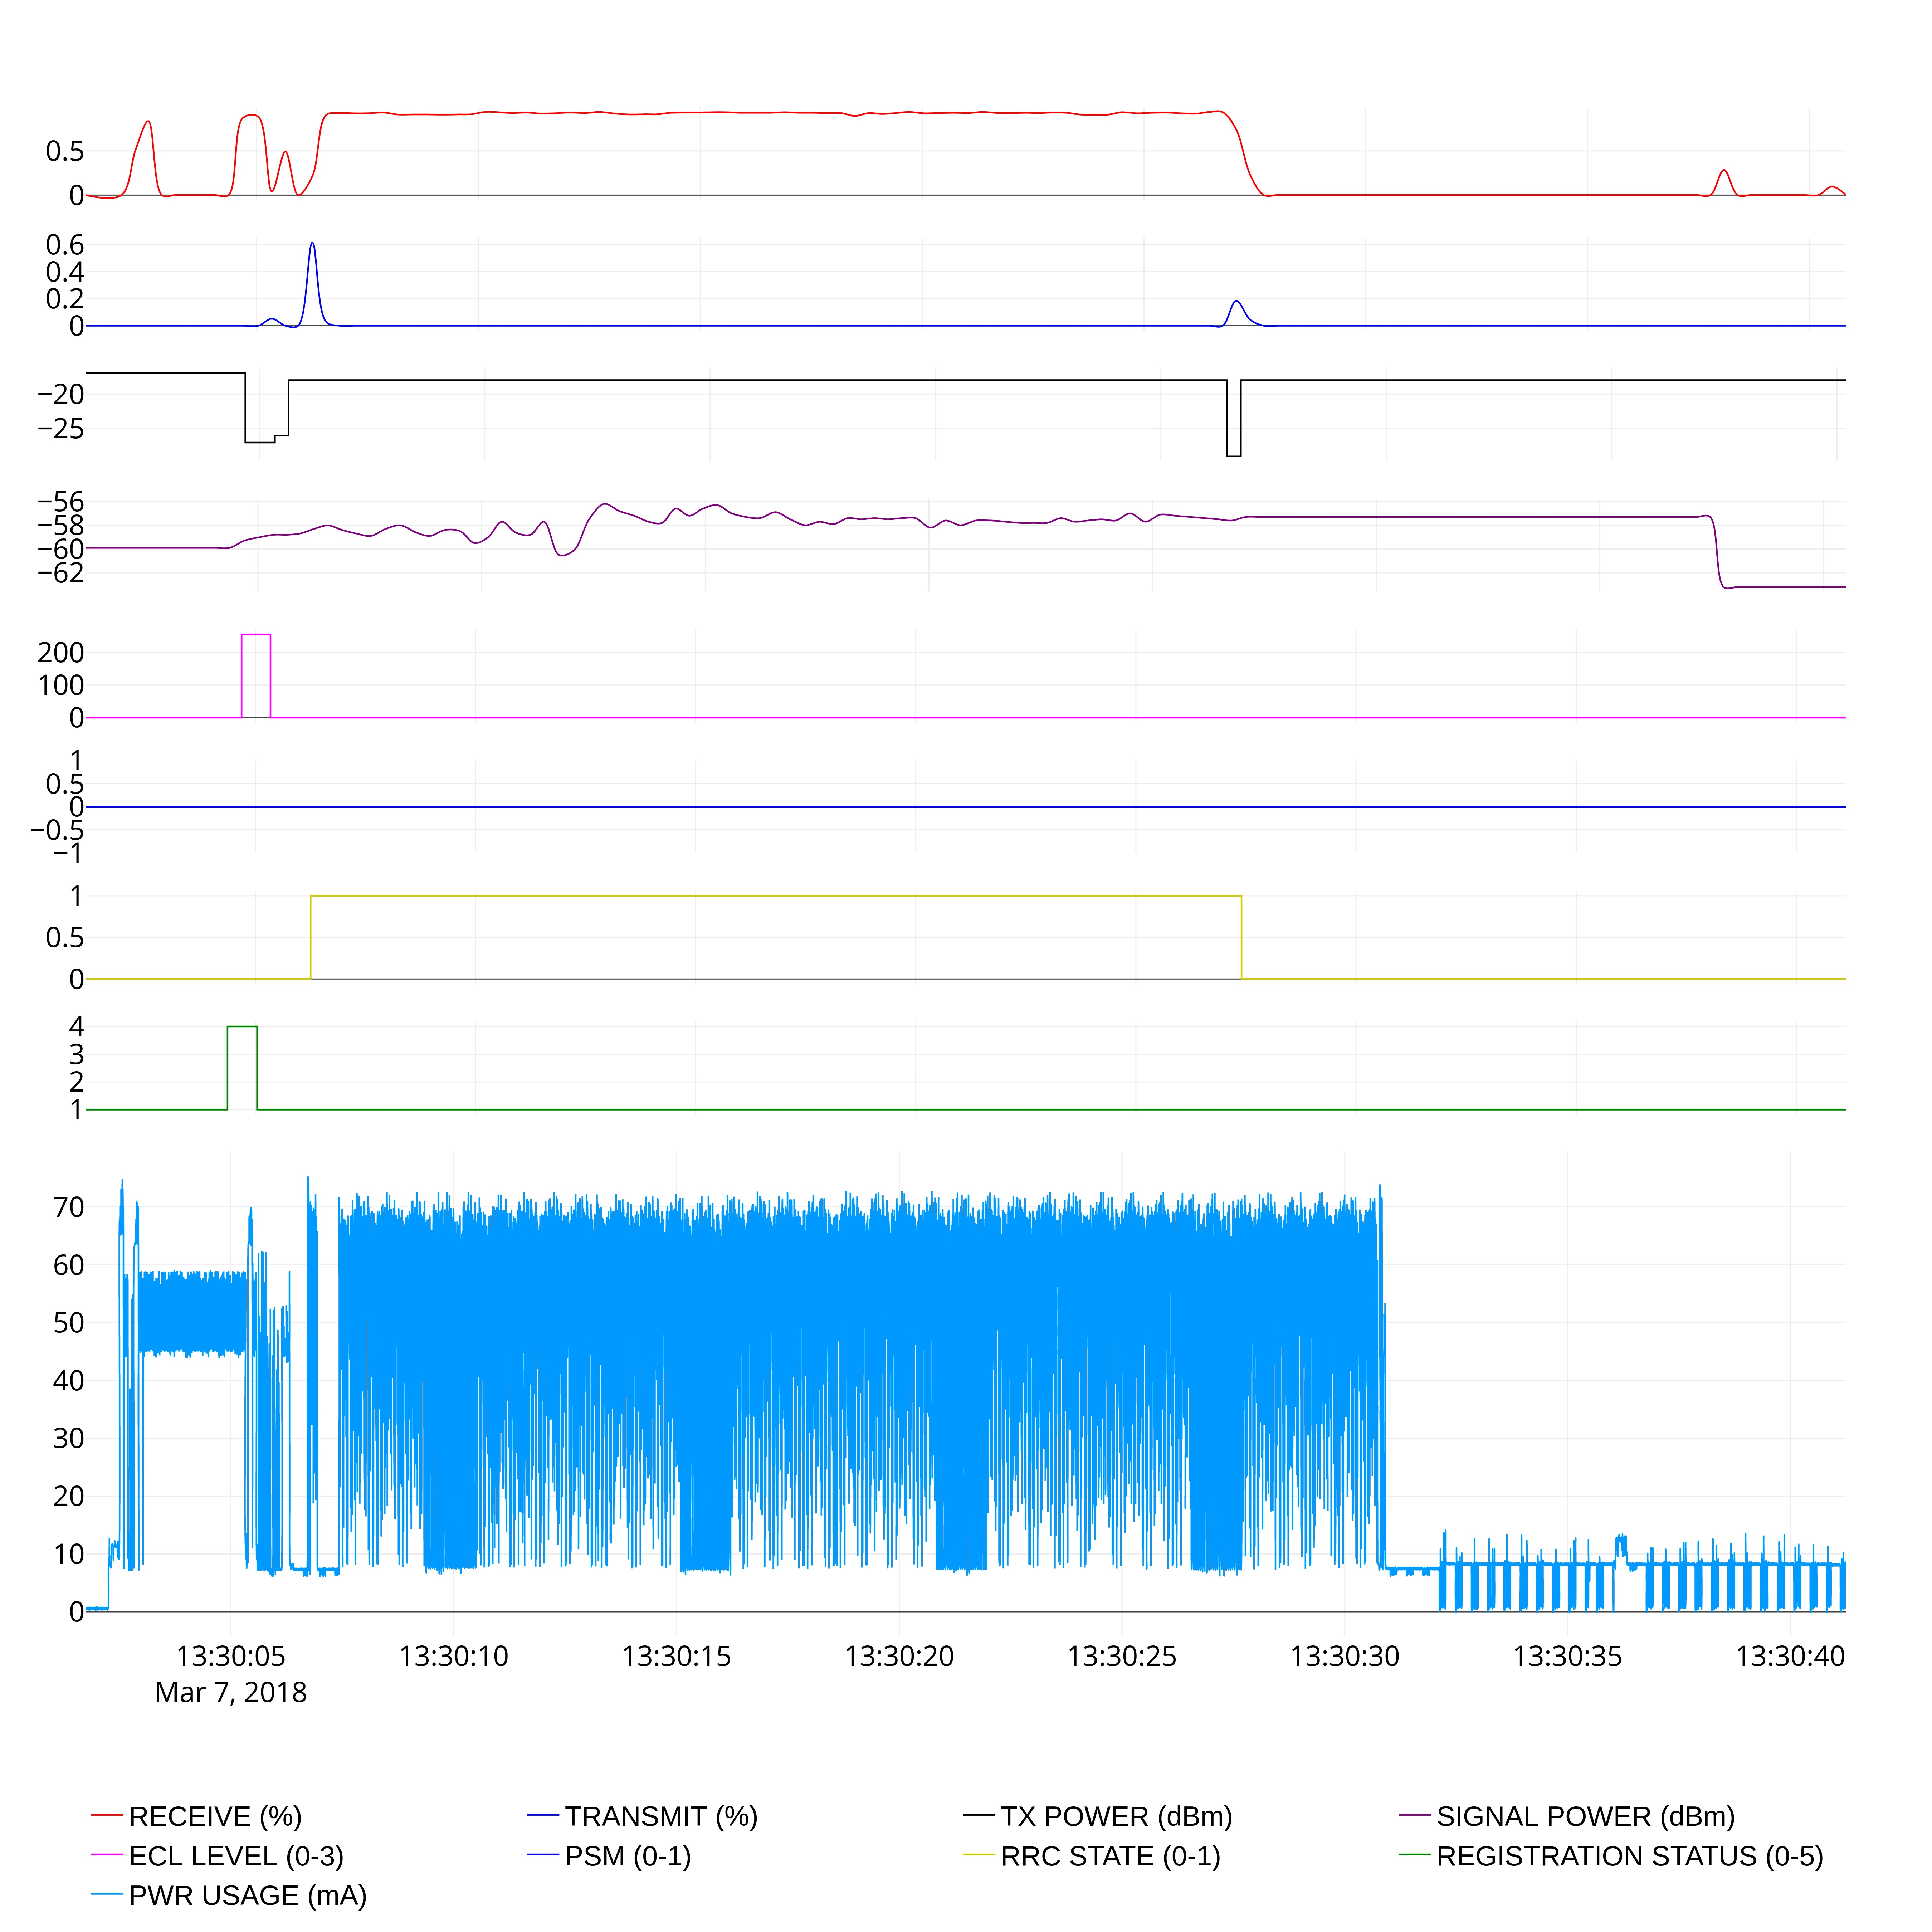
\includegraphics[width=0.9\textwidth, height=0.8\textheight]{/Users/henninghakonsen/Dropbox/Masteroppgave/thesis/latex/images/full_Q-FREE_TELENOR_5_02_2018-03-07_1_0x0_40_1_200.jpeg}
  \caption{1 x 40 Q-FREE, Telenor - device logging.}
  \label{figure:1x40_QFREE_TELENOR_1LOG}
\end{figure}

\subsection{\acrshort{ecl} level} \label{ssection:ecllevel}
\begin{figure}[H]
  \centering
  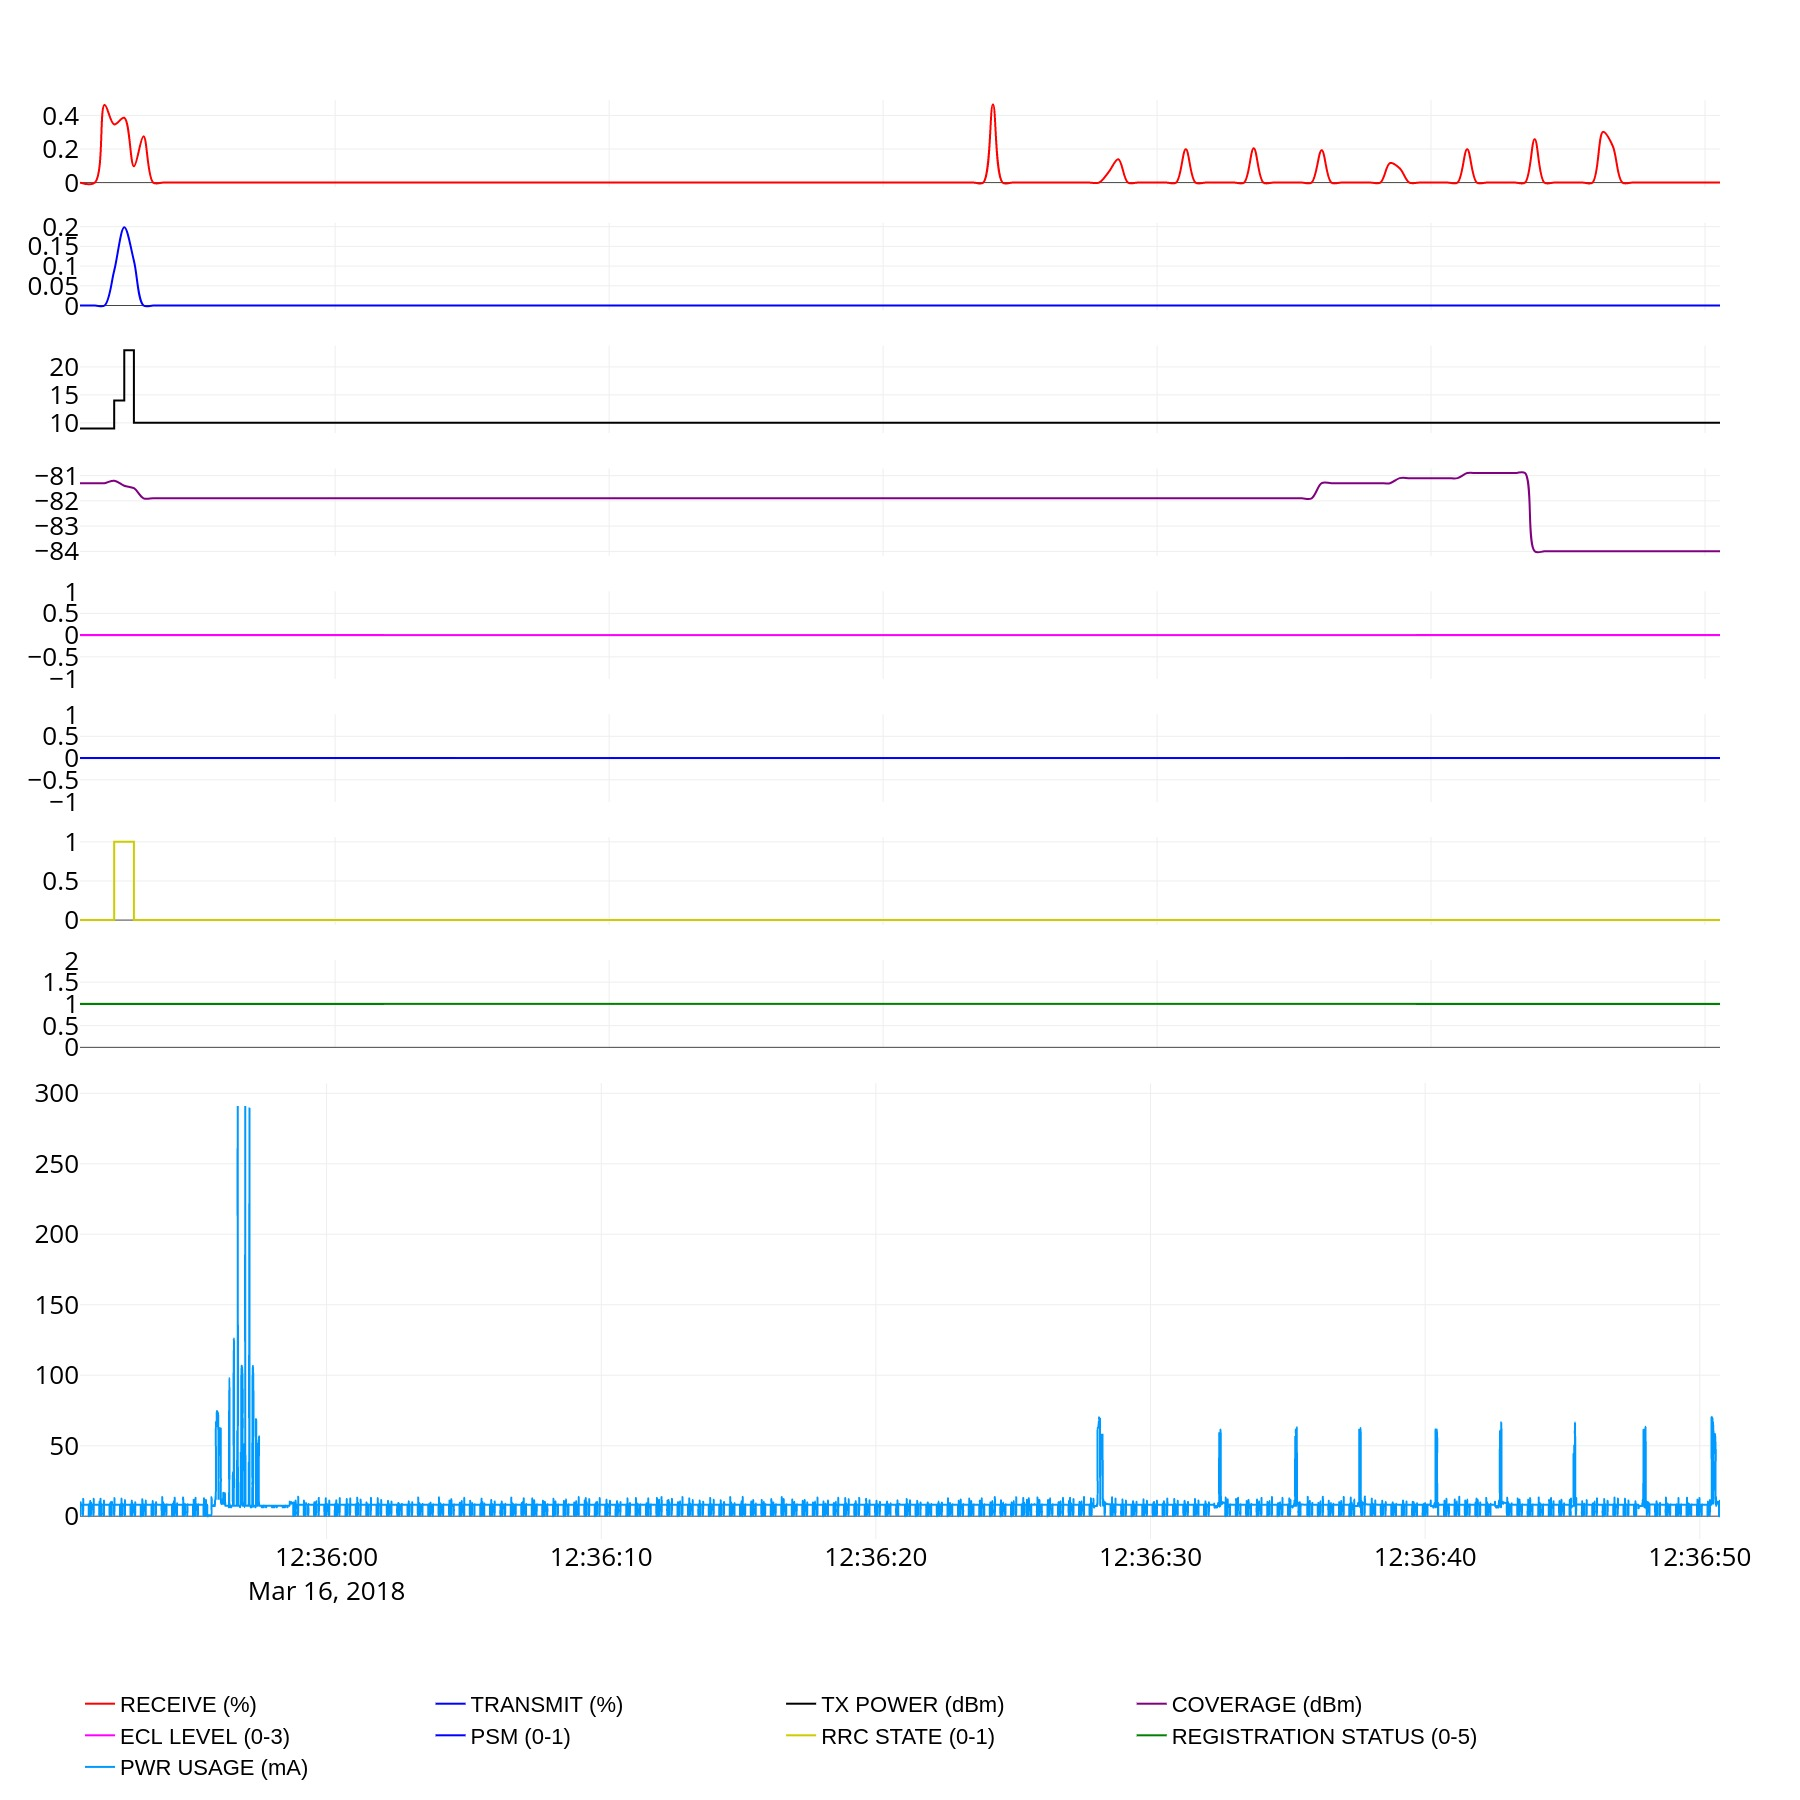
\includegraphics[width=0.9\textwidth, height=0.8\textheight]{/Users/henninghakonsen/Dropbox/Masteroppgave/thesis/latex/images/full_UiO_TELIA_5_02_precision_2018-03-16_1_0x2_60_1_50.jpeg}
  \caption{1 x 60 UiO, Telia - \acrshort{ecl} 0.}
  \label{figure:1x60_UIO_TELIA_ECL_0}
\end{figure}

\begin{figure}[H]
  \centering
  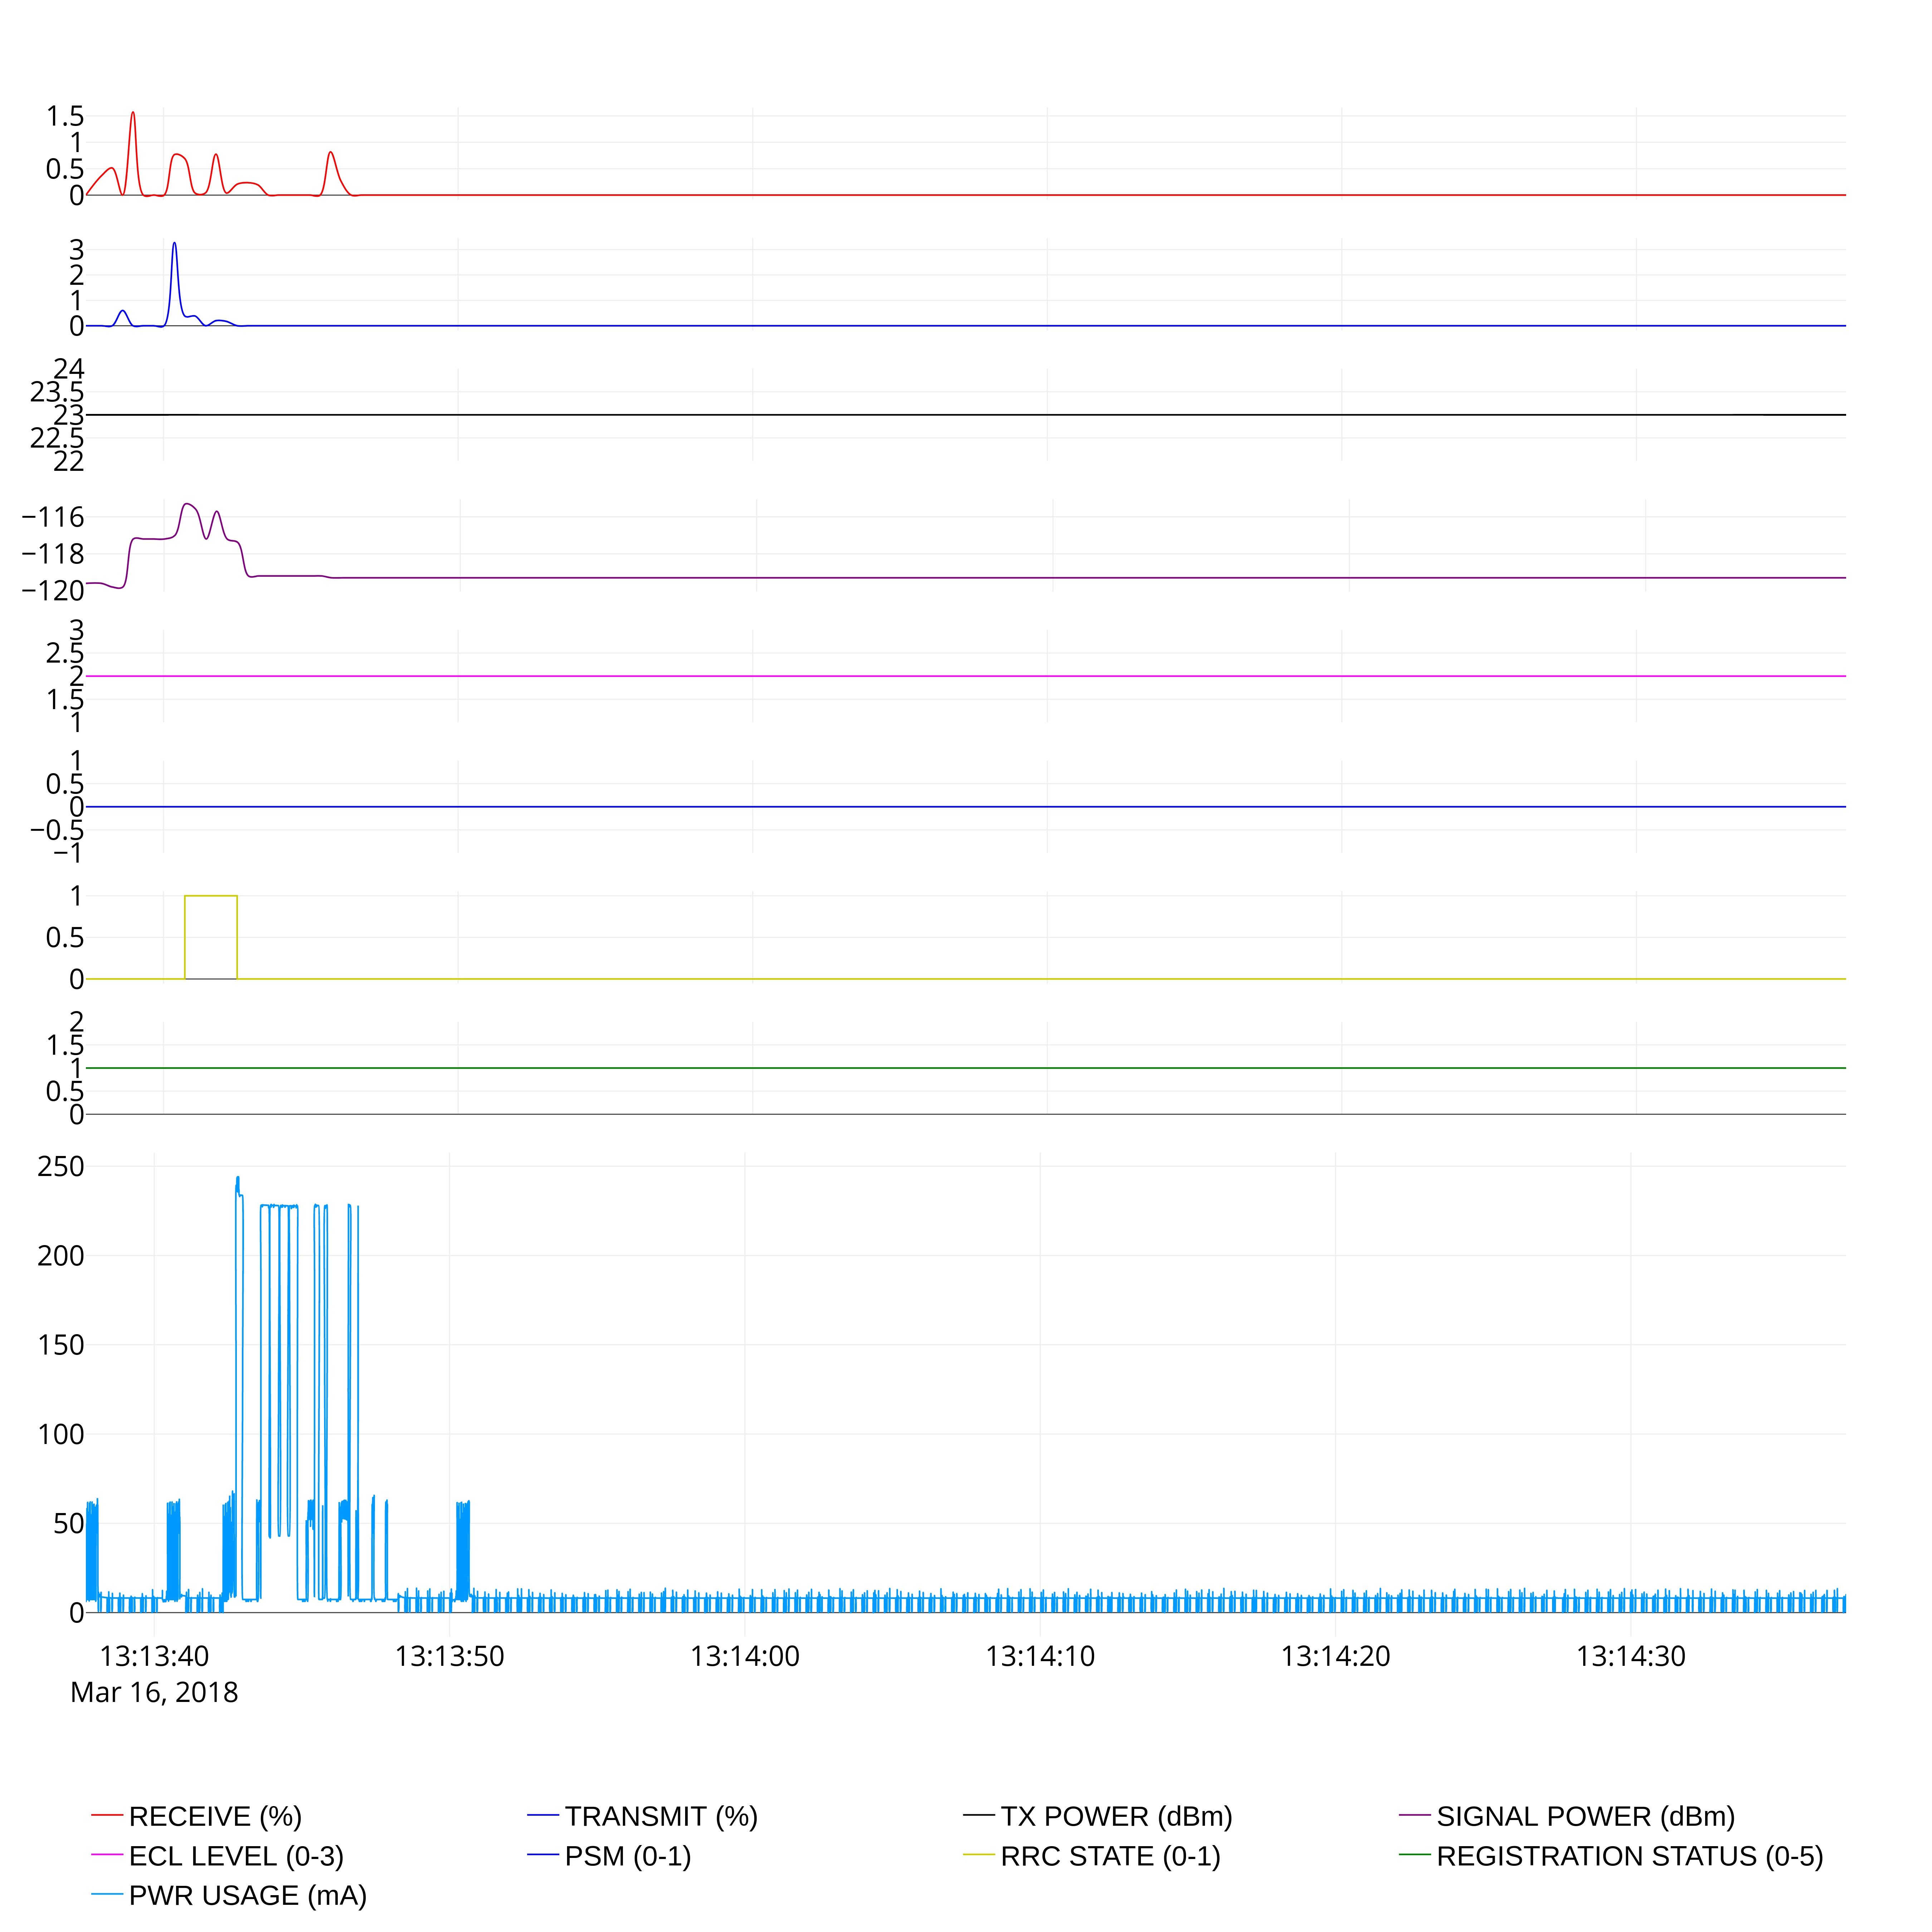
\includegraphics[width=0.9\textwidth, height=0.8\textheight]{/Users/henninghakonsen/Dropbox/Masteroppgave/thesis/latex/images/full_UiO_TELIA_5_02_precision_+30dBm_att_2018-03-16_1_0x2_60_1_50.jpeg}
  \caption{1 x 60 UiO, Telia - \acrshort{ecl} 2.}
  \label{figure:1x60_UIO_TELIA_ECL_2}
\end{figure}

\section{Long term tests} \label{section:longtermtest}
A device operating over long time is prone to many bugs and the quality of the software is essential. In this section we will give you an overview of how the network handles continuous transmits over a longer period. We have tested the device at all locations with both network providers where the device managed to connect to the network. We define long term test as a set of operations over a long period compared to the detailed tests, typically one or several days. When trying to test many scenarios, the test period per network provider and location is limited. However, the results are comparable to the short term tests and there are clear indications of the networks pros and cons. The reason for the long term tests is to monitor the normal behavior of the chip over a longer period, which would give us statistics at a more abstract level and combine the results with the short term tests. With this relation we will give you an overview of the most common states of a device and how different aspects reflect the behavior. We have had some problems logging correct behavior of the device over a long period. It seems that at random points in time it looks as if the device looses connection to the network resulting in \acrshort{ecl} level set to 255, and receive/transmit timers are reset. It is at this stage unclear what evokes this behavior, but one reason might be related to \acrshort{psm} periods as the device shuts down all internal processes only keeping the clock and some logic alive. We had some progress to this problem in late March when we used the program, \textbf{nbiot\_labtest.py}, for our long term tests. This program constantly pulls the chip for statistical data, hence we might assume that the device is more active. Even with this program we saw signs of the same behavior and because of this abnormality some of the results are harder to make sense of, especially receive/transmit time. However the results we got were very much like the results from the short term tests and we will use the good results to describe how the network performs.

Since the transmits towards the server contains all aspects of the long term process we will try to include more information about the specific periods in this test, rather than to split the results into categories. We think that you will gain more knowledge by seeing relations between coverage, latency and other statistical perspectives at the same time. Most of the figures included in this section is taken from the web application so if you are unfamiliar with the format please refer to section, \vref{sssection:layout}, for a more detailed description of the graphs. For the best experience we advice you to use the web application to view the data, but we will include the most interesting findings in each apprioriate section.

\subsection{Coverage and latency}
One of the key features of \acrshort{nb-iot} is the extended coverage. Devices should have good reception in normally bad coverage areas, such as tight city areas and far away mountain sides. The transmit power is ${+23 \acrshort{dbm}}$ which is very good, considering that a theoretical ${+3 \acrshort{dbm}}$ step is actually doubling in power output. The coverage is not only related to the distance between the \acrshort{ue} and the base station, but also the obstacles between. By looking at the map, \vref{figure:map_qfree}, we can see that the distance between the \acrshort{ue} and base station at UiO and Q-Free is low, but the reception was quite different. At Q-Free, with Telenor, the reception was normally at ${-60 \acrshort{dbm}}$, while at UiO with Telia, the reception was normally at ${-80 \acrshort{dbm}}$.
The main reason for the big difference is due to what lies between the sender and receiver. At Q-Free there are very few obstacles, hence the signal is passed directly to the base station. At UiO there are several builds between the \acrshort{ue} and the base station, resulting in lower reception. It would be interesting if Telenor also had a \acrshort{nb-iot} enabled base station at the same location at UiO so that we could compare the two network providers more closely. We might assume that the two network providers use the same technology to offer \acrshort{nb-iot}, but it is probably not from the same producer which might explain the big difference in reception as well.

In the following two sections we will give you insight in two longer transmit sequences. Because of the issues we have had with the long term test we have focused mostly on one of the sequences with Telenor since their network is the most stable of the two. In section, \vref{ssection:ecl_255}, we discussed what happened on the device at the occurrences of these reconnection periods.

\subsubsection{Telenor}
We will begin looking closely at a transmit session over 5 days, 23.03-28.03, from UiO with Telenor's network. We have included two figures taken from the web application, \vref{figure:uio_telenor_lc} and \vref{figure:uio_telenor_stat}, which we will use to point out certain aspects of the normal transmit process. Looking at the first section we see a steady line for both coverage and latency. The coverage is around ${-95 \acrshort{dbm}}$ and the latency ranges from 1.5 seconds to 3.5 seconds on average. We classify this as quite good coverage and resembles normal behavior. A thing we noticed is the flow of the latency line. We can see a clear interval between the high latency spikes and the low. We have not been able to find the origin of this behavior, but it most likely has something to do with the process in the core network since both the server and the client in this setup behaves the same way at all times. Another indication that it originates from the core network is that my supervisor, Q-Free's R\&D manager, Ola Martin, also has seen this behavior in his tests \cite{person:ola}. Another interesting thing to view is receive/transmit time in the second figure. Looking at the transmit graph we can see that a normal transmit uses approximately 0.3 seconds which is relatable to the short term tests. Also looking at the receive time graph the normal receive time between two transmits are around 21 seconds since these transmits were not using the \acrshort{rai} flag. This is also very well in terms of what we saw in the short term tests. This is useful information since we now know that this is not only a one time occurrence, but is actually the normal behavior of a receive/transmit process without \acrshort{rai} set.

Looking at the same period we can see three clear latency spikes up towards 10 seconds without any indication of bad reception. However at each latency spike we can see a similar spike in receive time and this indicates that something happened in the network which the device needed to listen in on, hence the transmit towards the server is delayed. The specification states a maximum latency of 10 seconds, so these transmits are on the edge of what is normal behavior. After a while, around 16:00 23.03, we see that the trend shifts. The coverage is the same, but the latency suddenly fluctuates up towards 5-6 seconds and this happens with the same interval flow as previously. To try to see if the behavior is related to the test program we tried to restart the program at, 20:36 25.03, now with \acrshort{rai} flag set. The same behavior continued until I restarted the development kit at 14:00 26.03, where we can see that the coverage and latency normalizes to what we classify as normal behavior. A thing you might have noticed is the drop in receive/transmit time. There is a noticeable behavior change in receive time when \acrshort{rai} is set and this is very logical since the device goes to sleep directly after the transmit process has finished. Even though the transmit process only covers \~0.3 seconds there are still some overhead related to the transmit process so the typical receive time for Telenor is 2-3 seconds, which is approximately ten times lower than with \acrshort{rai} not set. It is hard to see from the figure, but the transmit time is also reduced to some extent while using the \acrshort{rai} flag. This is related to lowering the network communication overhead of a transmit. The average transmit time with \acrshort{rai} set is approximately 0.15-0.2 seconds, which is around 50\% less than without \acrshort{rai} set. Since the transmit process involves higher power usage a decrease in time usage is valuable.

From 10:00 to 12:00 26.03 we can see three spikes in the receive time, which might indicate trouble with the connection towards the \acrshort{enb}. If the device thinks it looses connection it will remain in RRC mode, hence receive data on a regular basis. This is not something we want happening since it consumes very much power. We will elaborate what could be done at such events in section, \vref{section:guidelines}.

At 12:14 27.03 we added a ${-20 \acrshort{dbm}}$ attenuator to the development kit hence the coverage spiked up to around ${-120 \acrshort{dbm}}$. The reason to why we add attenuators is because it is interesting to see how the network performs in these conditions, even though it will hopefully not be the case of most applications. First of all we can see that the base latency is around the same, but the interval we saw earlier is not as clear as before and the overall latency is higher. More interestingly is to watch the receive/transmit time graphs, as they show a whole different operation than earlier. We begin looking at the graph for transmit time, where we can see that the device retransmits packets very often. We see that many transmits uses around 2 seconds, while others are between 4-8 seconds. This is close to what was described in section, \vref{ssection:transmitprocedure}, meaning that in addition to time spent in transmit mode the transmit it self also uses maximum power for each transmit. This behavior is extremely battery deficient and will cause poor lifetime. There is one spike of transmit time at 23.5 seconds with a related latency at 24.25 seconds.

Moving over to the graph with receive time we can see that the minimum receive time is still 2-3 seconds, but now the line is not very stable. We see more tendencies to spikes as the device has to use more time communicating with the network because of the poor reception. However the receive time is not affected to the same degree as the transmit time and is kept under 10 seconds for most of the transmits. Looking at the two graphs the transmit time increased with approximately ${2.5S / 0.2S = 12.5}$, while receive time only increased with approximately ${5S / 2.5S = 2}$. This is not surprising since we know that at \acrshort{ecl} level 1 and 2 the device retransmits packets frequently to achieve higher receive rate at the \acrshort{enb}.

\begin{figure}[H]
  \centering
  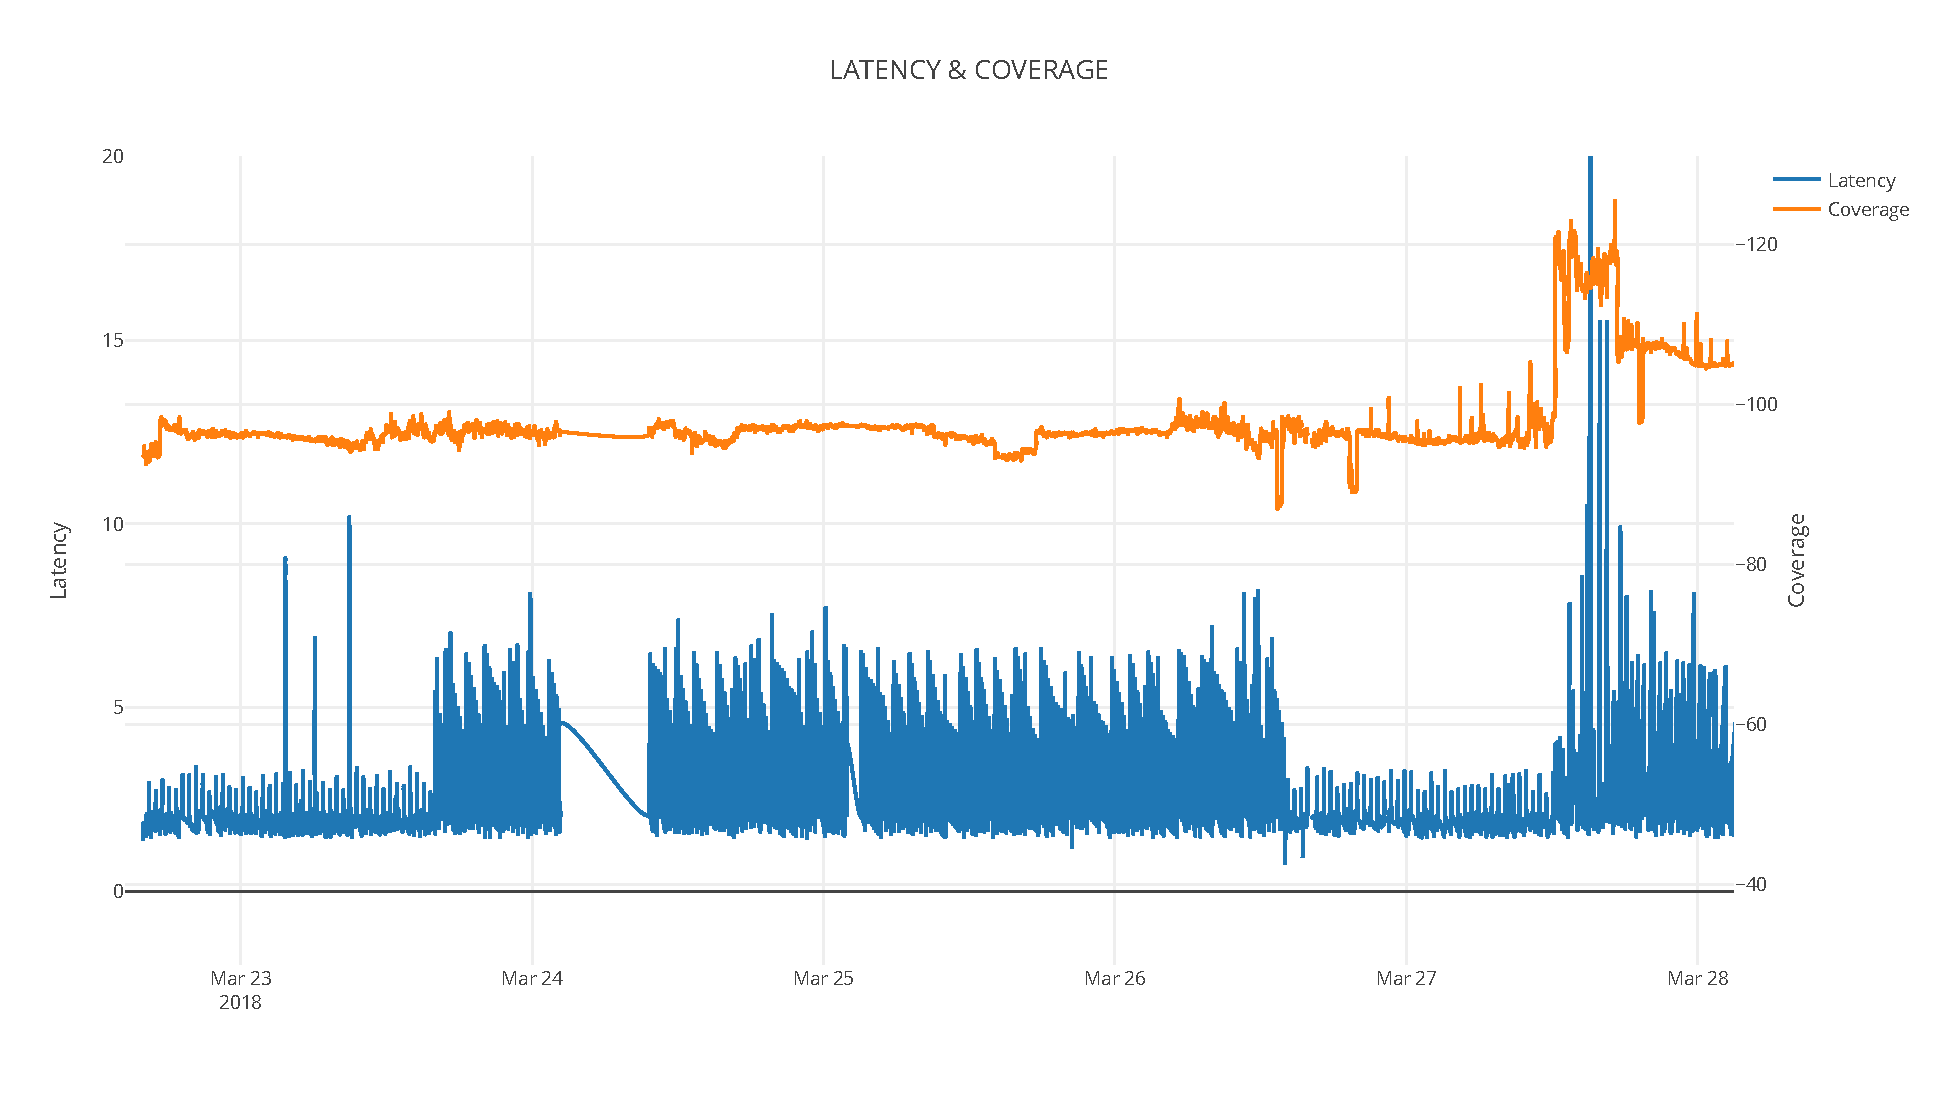
\includegraphics[width=0.9\textwidth, height=0.4\textheight]{/Users/henninghakonsen/Dropbox/Masteroppgave/thesis/latex/images/uio_telenor_lc.pdf}
  \caption{Telenor - latency and coverage. Visit, \href{http://158.39.77.97:9000/\#/nodes/id2}{webapp}, for more details.}
  \label{figure:uio_telenor_lc}
\end{figure}

\begin{figure}[H]
  \centering
  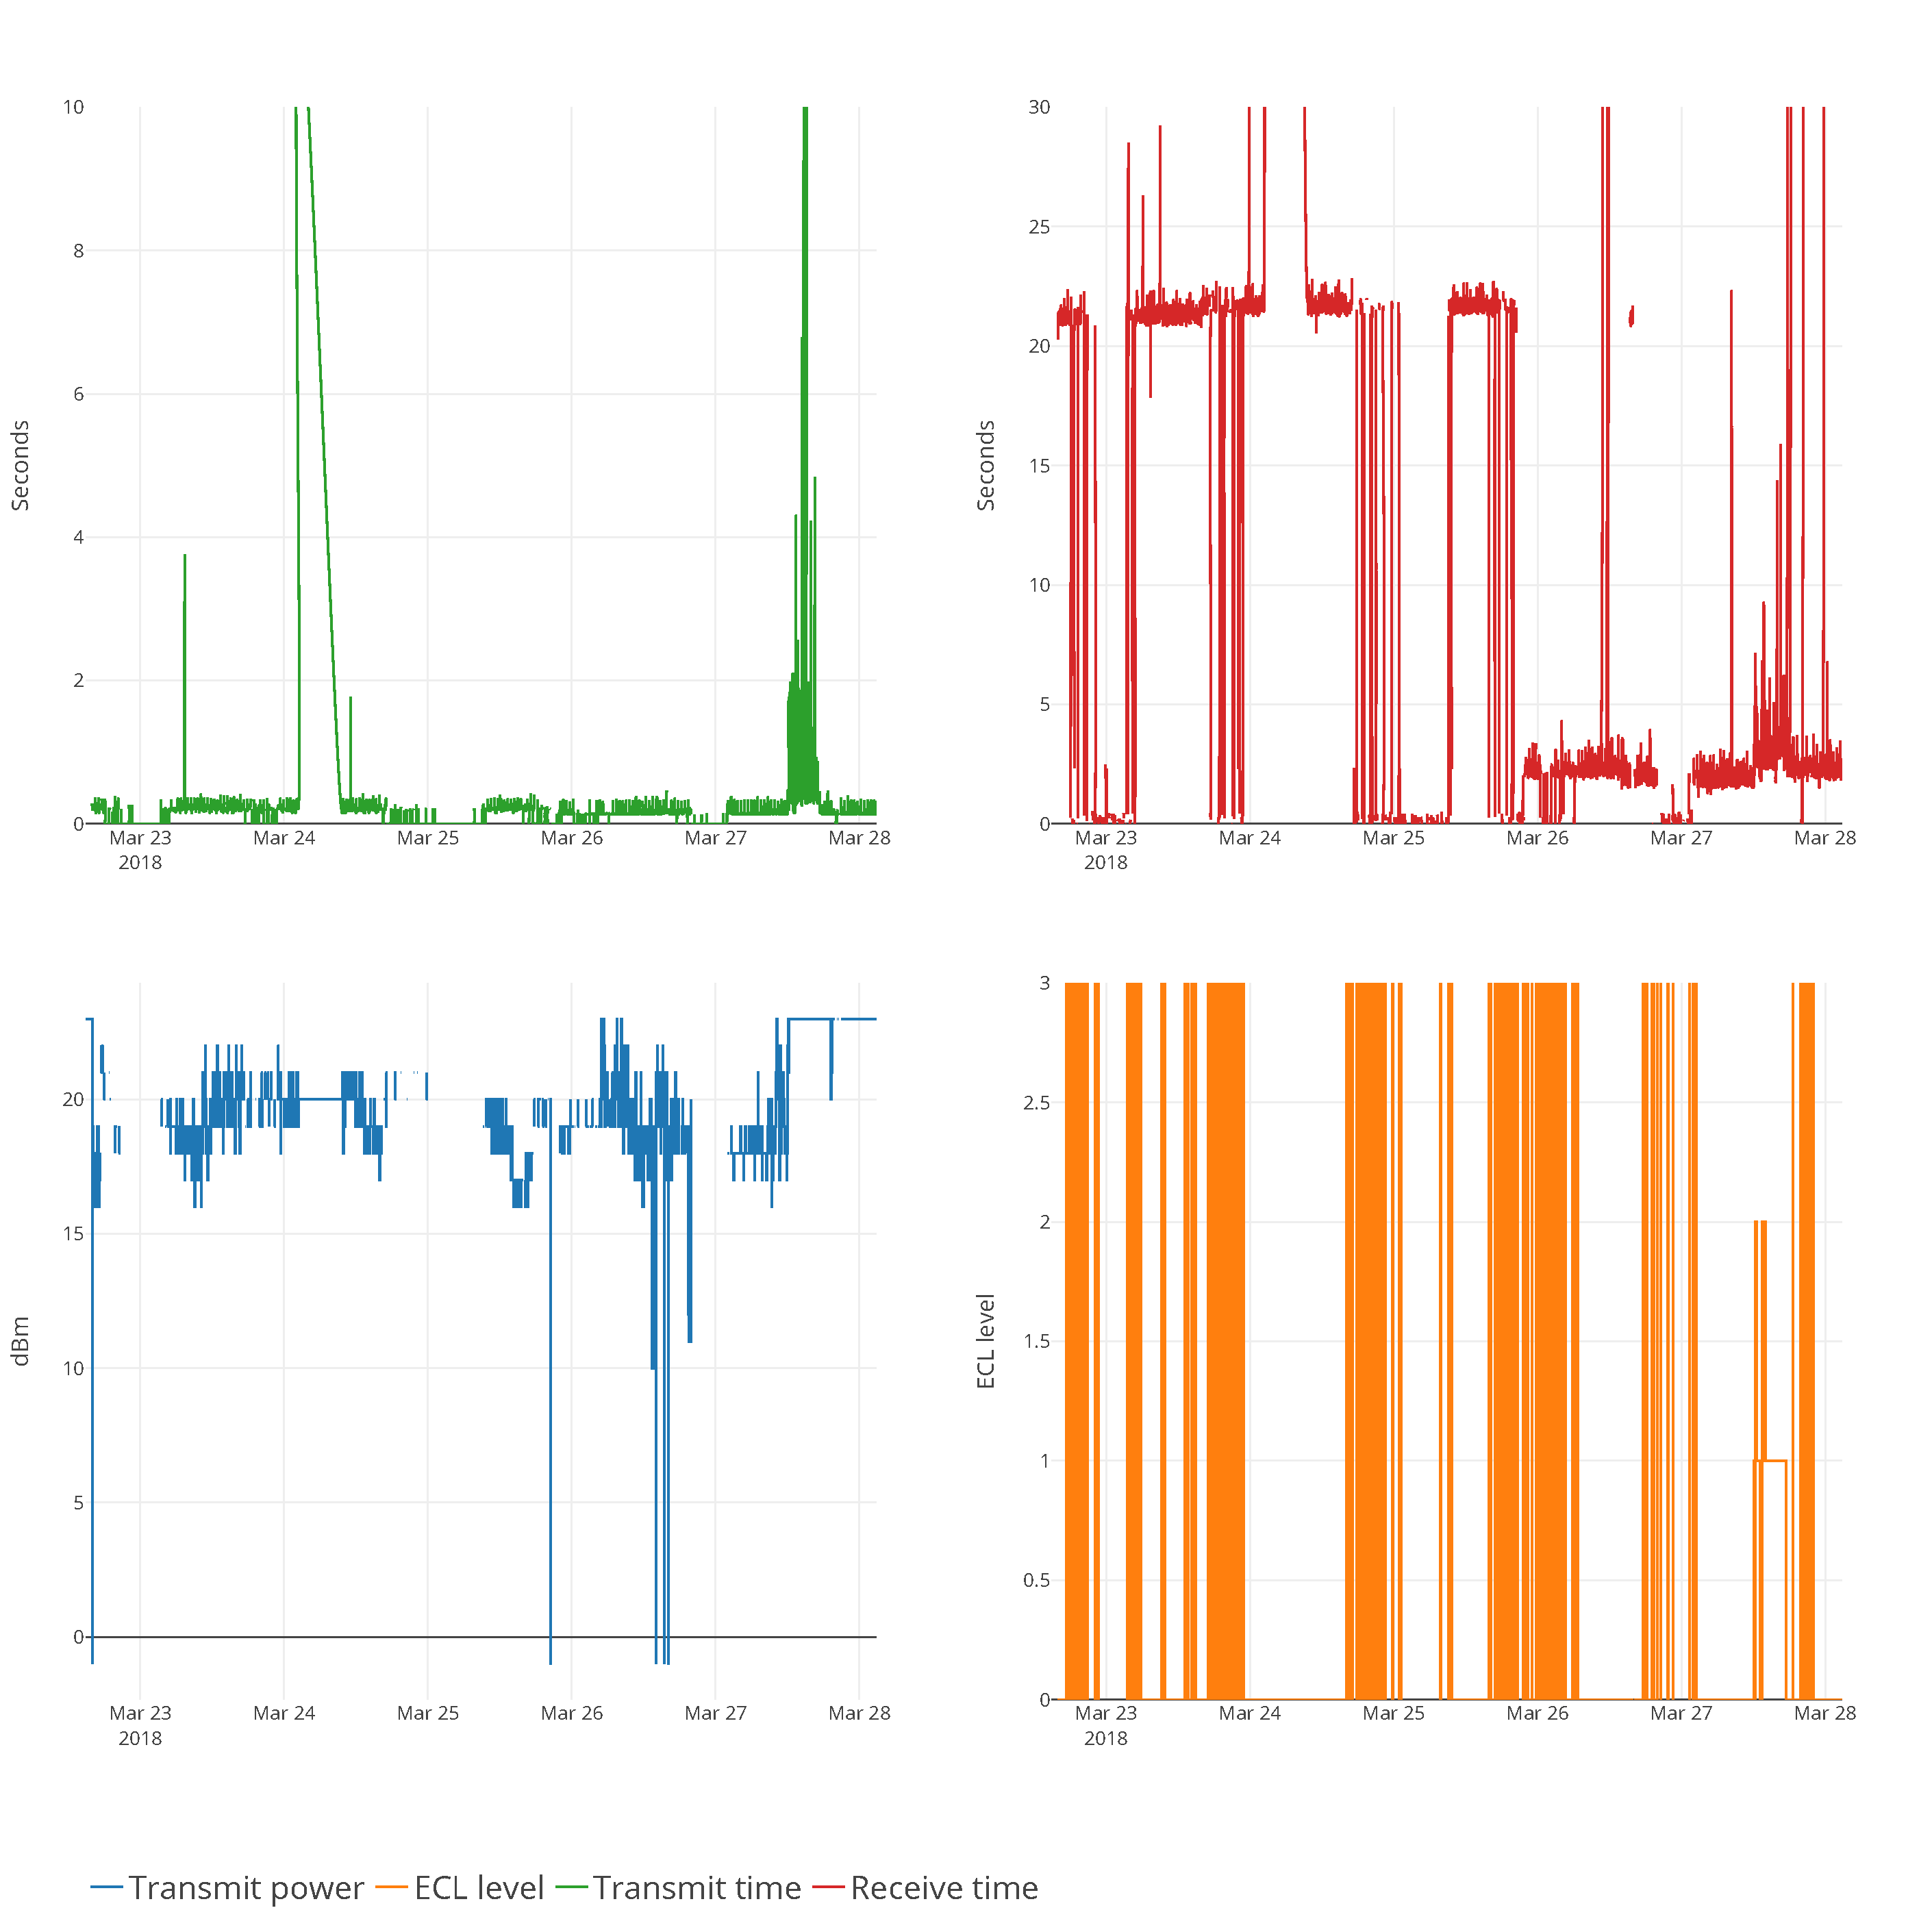
\includegraphics[width=0.9\textwidth, height=0.4\textheight]{/Users/henninghakonsen/Dropbox/Masteroppgave/thesis/latex/images/uio_telenor_stat.pdf}
  \caption{Telenor - statistics. Visit, \href{http://158.39.77.97:9000/\#/nodes/id2}{webapp}, for more details.}
  \label{figure:uio_telenor_stat}
\end{figure}

\subsubsection{Telia}
Transitioning over to Telia we will look closer at one of the sequences recorded with Telia's network at UiO, from 20.03.18 to 23.03.18. The setup is similar to the one discussed in the section over and there are obvious differences as we have seen earlier. We have included two figures to illustrate the result, \vref{figure:uio_telia_lc} and \vref{figure:uio_telia_stat}.
Looking at the beginning of the first figure we see that the graphs are comparable to Telenor's result. However, as you might have noticed most of the transmits are less stable, which affects the results. Since we don't get any feedback from the network it is hard to state the reason for this instability, but referring to section, \vref{section:market}, we know that Telia deployes \acrshort{nb-iot} in-band within their \acrshort{lte} deployments. We know that if there are many users in a certain area, this can cause poor reception and latency \ref{ssection:operationmodes}, hence our results reflect what might be this kind of behavior.

In addition the problem with reconnection is worse with Telia's network. This is probably related to the instabilities we have seen. Since the results are degraded we want you to keep in mind the results from the previous section as a kind of benchmark to what we believe is the closest to stabile behavior at this moment. However, the results from Telia shows an improvement in time spent in receive mode with \acrshort{rai} not set. Looking closer at the last part of the graph we see a steady sequence without reconnections. This show us that when the transmit process behaves properly the device spends around 6 seconds in receive mode between each transmit. As stated in section, \vref{ssection:generaltest}, Telia uses approximately 60\% less time in RRC mode resulting in lowered power consumption. At first we thought that this was the reason for the instabilities we saw, but we see the same behavior with \acrshort{rai} set. When \acrshort{rai} is set the two networks perform more or less identical if we only consider transmit and receive time.

\begin{figure}[H]
  \centering
  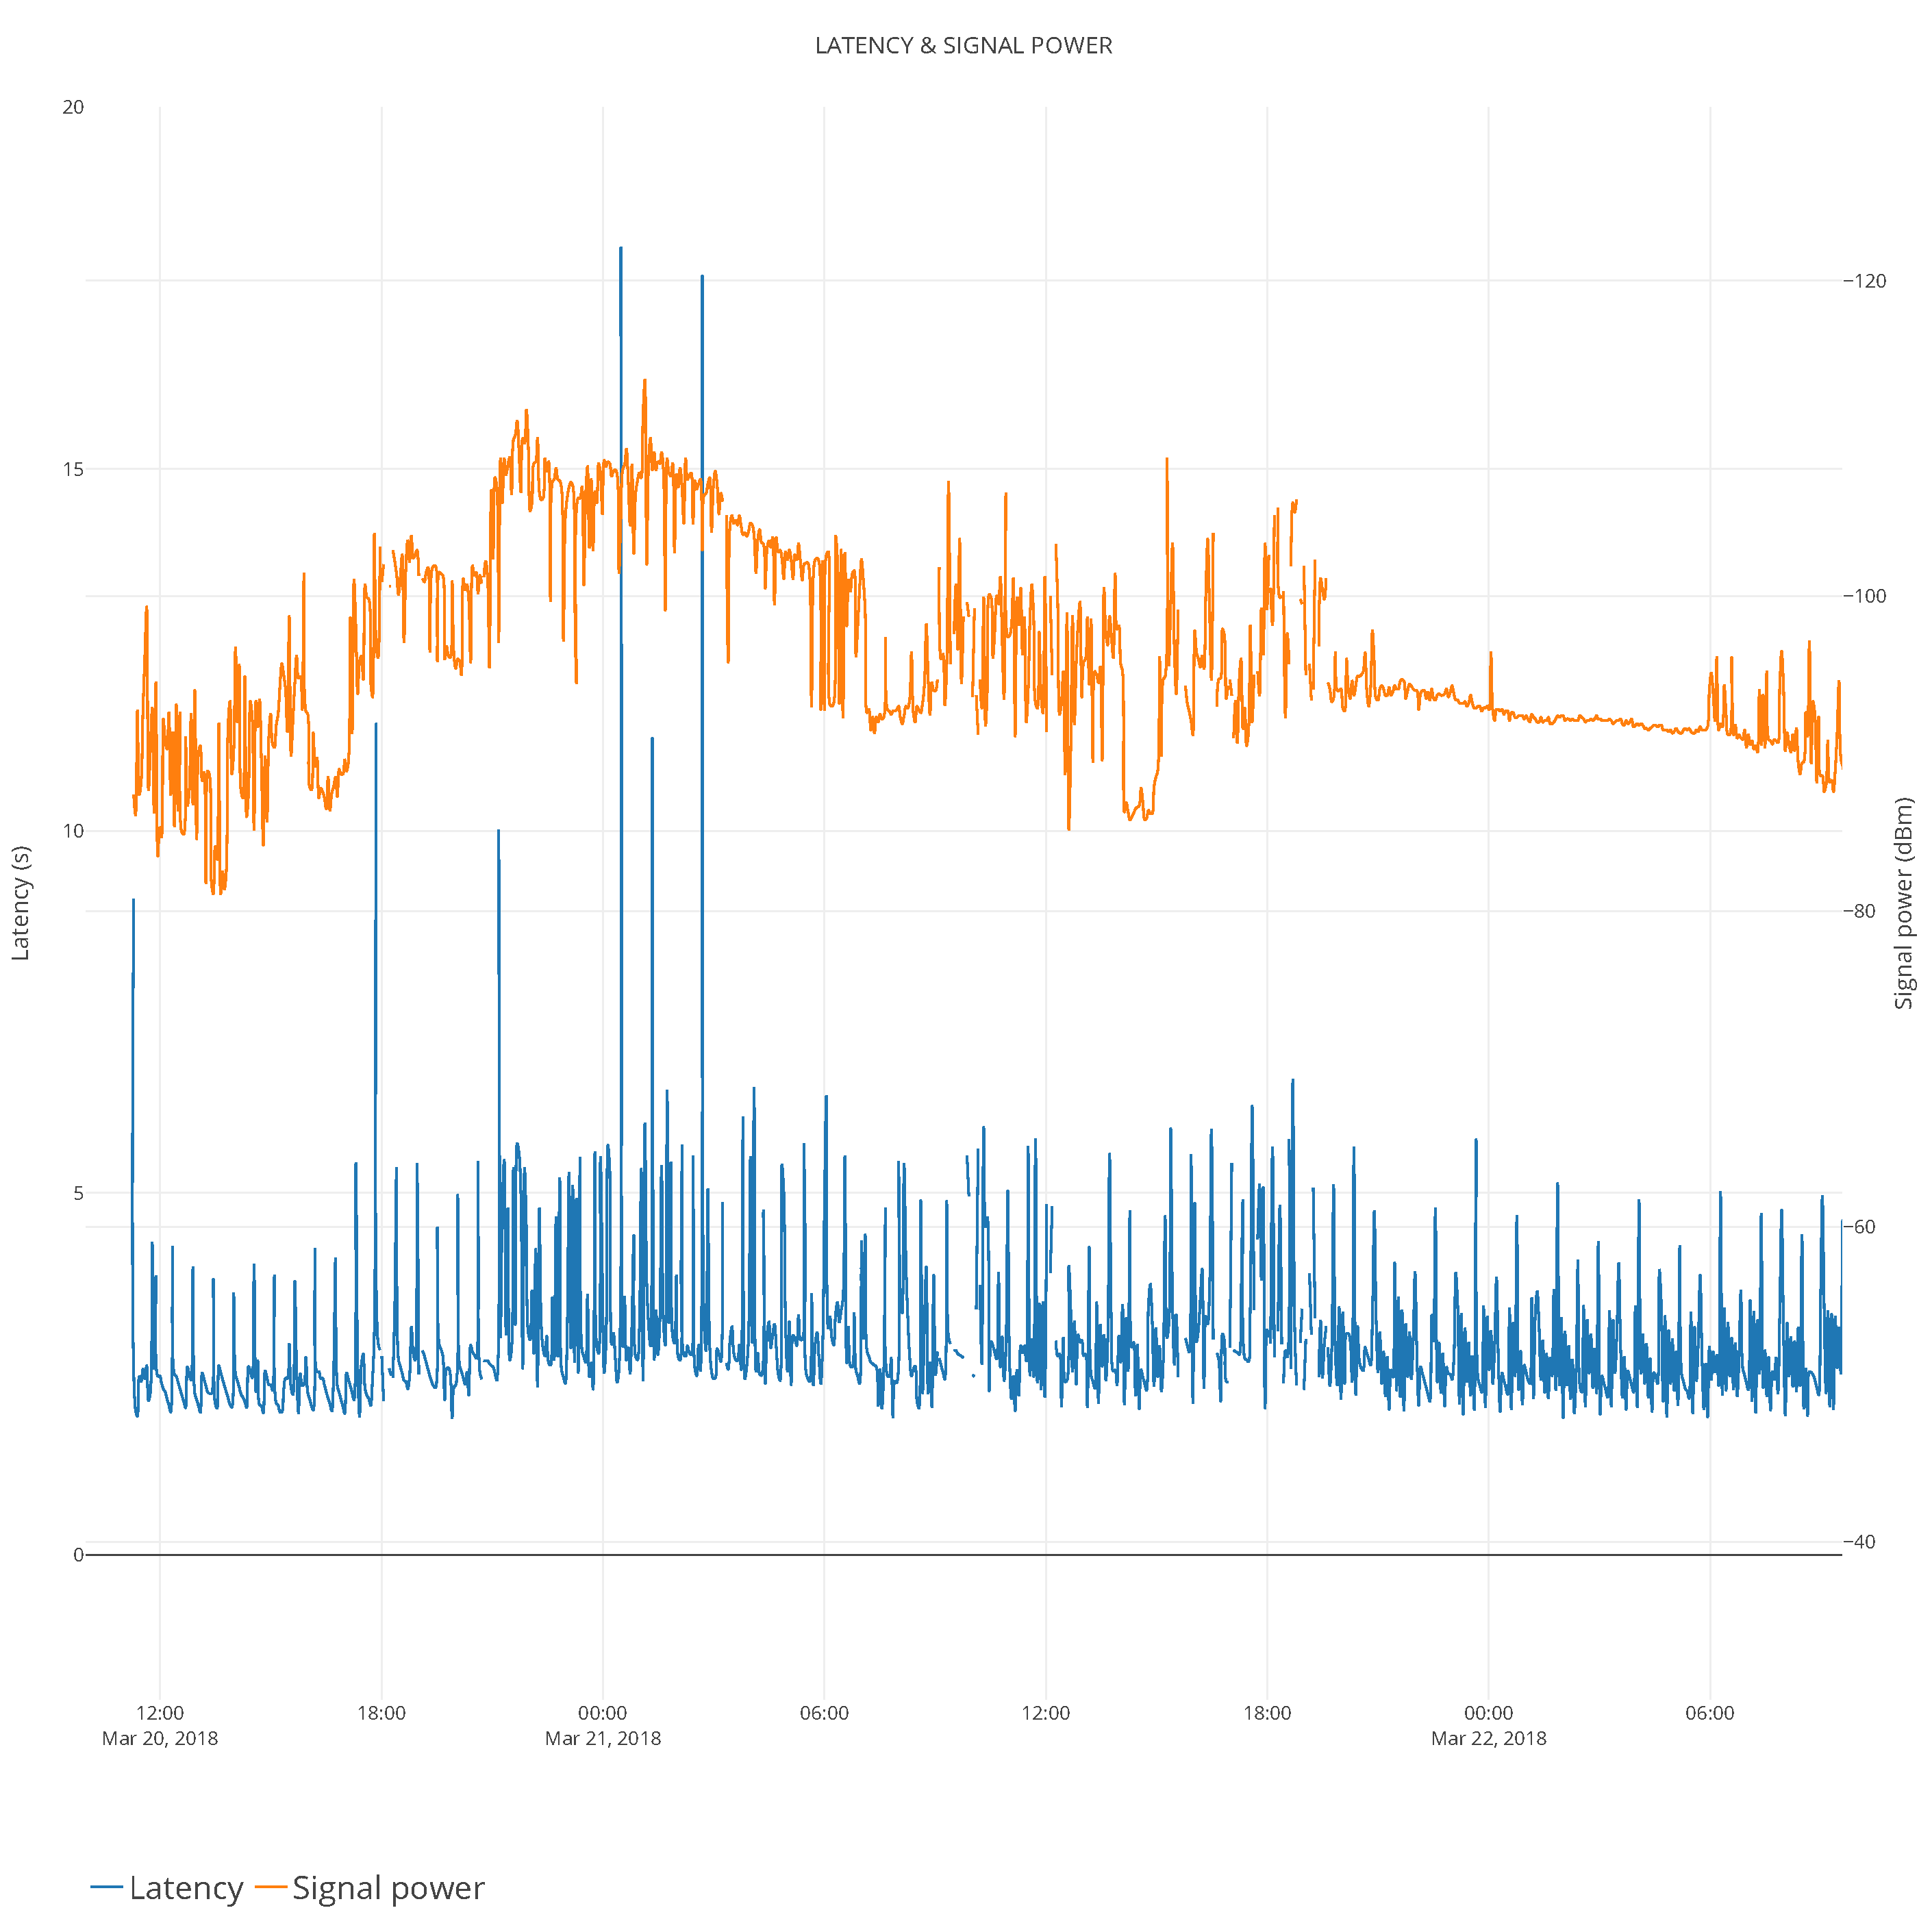
\includegraphics[width=0.9\textwidth, height=0.4\textheight]{/Users/henninghakonsen/Dropbox/Masteroppgave/thesis/latex/images/uio_telia_lc.pdf}
  \caption{Telia - latency and coverage. Visit, \href{http://158.39.77.97:9000/\#/nodes/id1}{webapp}, for more details.}
  \label{figure:uio_telia_lc}
\end{figure}

\begin{figure}[H]
  \centering
  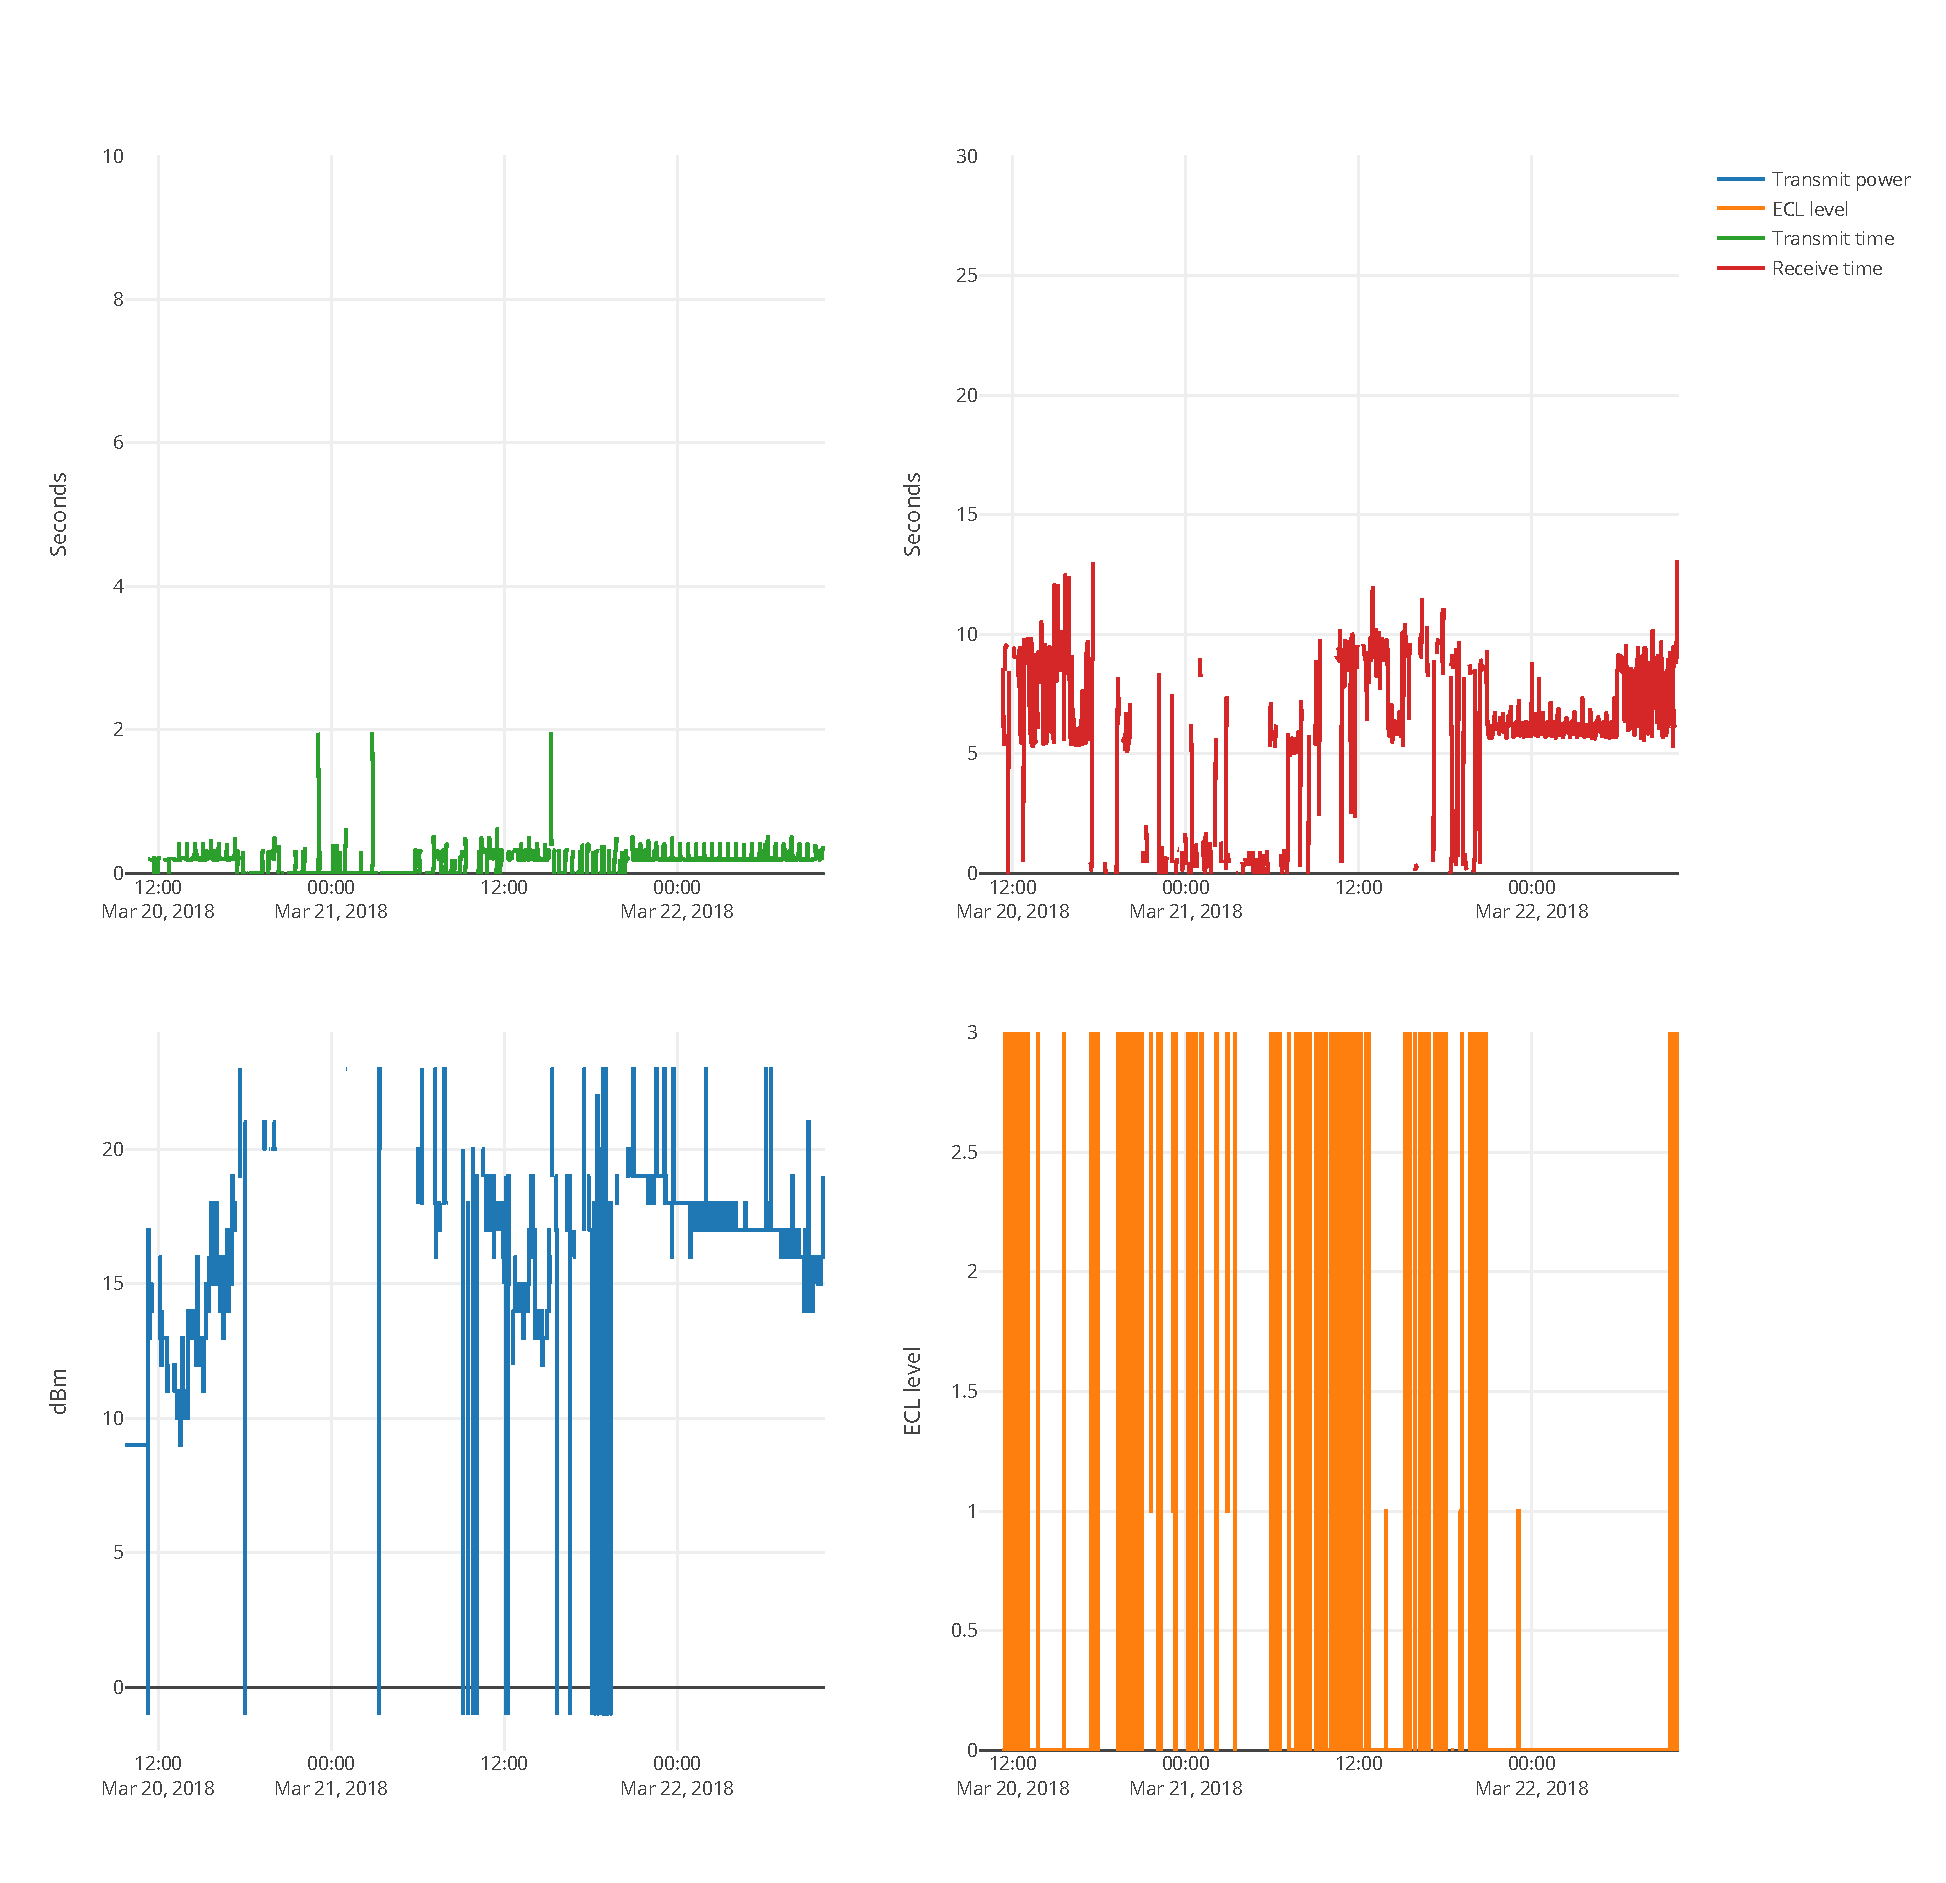
\includegraphics[width=0.9\textwidth, height=0.4\textheight]{/Users/henninghakonsen/Dropbox/Masteroppgave/thesis/latex/images/uio_telia_stat.pdf}
  \caption{Telia - statistics. Visit, \href{http://158.39.77.97:9000/\#/nodes/id1}{webapp}, for more details.}
  \label{figure:uio_telia_stat}
\end{figure}

\subsection{Cell selection}
When the device has bad reception it will try to reselect which cell it is connected to. We wanted to test how this affects the battery lifetime since this might happen frequently if the device is located equally far from two cells with approximately the same signal power. It might then jump back and forth between these cells which could drain the battery. However, because of the limited \acrshort{nb-iot} enabled \acrshort{enb}'s we were not able to test this hypothesis. We know that an attempt to connect to a network leads to higher power usage [\ref{ssection:reboottest}], hence reconnecting to a new \acrshort{enb} will probably use a similar amount of power.

\subsection{\acrfull{tsr}}
For an \acrshort{iot} application receive rate is not a priority, but it is important with stability and high uptime. All transmits towards the server includes a message id and we have used this to generate statistics about the transmit success rate. The program \textbf{uptime.py} takes in three parameters, node id(-c), start date(-start) and end date(-end). If you specify the start and end dates the program will only include data within the given period. This option came handy due issues related to the hosts of the server some of the sequences has interrupts even though the device has continued transmitting data to the server.
The program calculates the transmit rate for sequences with a total number of transmits higher than 5 for the given period an prints a summary of the results. We have investigated all continuous sequences and used that to base our results upon. In listing, \vref{code:uptimerun}, you can see the output of one of the results, which displays data for id3 between \textbf{2018-03-13T15:00:00+02:00} and \textbf{2018-03-15T20:00:00+01:00}. Here we can see that in this period we found one sequence with a total transmits of 438 and actual received transmits of 426, which results in a \acrshort{tsr} of 97.26\%.

\begin{lstlisting}[caption={uptime.py example}, label={code:uptimerun}, language=Bash]
  Statistics about collection:  id3
  Transmits:  438
  Received transmits:  426
  Uptime:  97.26027397260275
  Total uptime:  [438. 426.  97.26027397]
\end{lstlisting}

We have looked at the sequences from UiO and can see that the \acrshort{tsr} for Telenor and Telia is pretty similar to the listing example. We see that some packets are lost, which surprised us. Considering the number of devices connected to \acrshort{nb-iot} at the point of the tests, we should have seen a higher \acrshort{tsr}. A packet loss of \~3\% is not very high, but if we imagine devices located in cities with device density of the technical specified limit of 50 thousand, the packet loss will probably increase resulting in degraded quality of service. We don't want the developers to have to implement retransmit logic in their applications so it will be interesting to see how the \acrshort{tsr} changes as more devices connect to the network.

\section{Deviations} \label{section:deviations}
\subsection{Imprecise clock}
With the command \textbf{AT+CCLK?} we get the time from the network. The timestamp is normally precise, but we did see that after a while that the time skewed and the latency on the server became negative. The first hours of transmits were however precise and we saw that the time fetched from the network was good enough for some applications. With the hardware and software of our test chip it was not possible to sync the clock at specific intervals, but this would be necessary if you wanted to use the internal clock.

\subsection{Imprecise \textbf{NUESTATS}}
We believe that \textbf{NUESTATS} has given us great feedback about the behavior of \acrshort{nb-iot}. As stated, the command is not 100\% accurate and we did also see certain issues related to \acrshort{ecl}, receive/transmit time, but in the end, when we combine the results from our test applications it is clear what the device actually does. As stated in sections, \vref{ssection:manufacture} and \vref{section:longtermtest}, the short term tests gives the best picture of the state of the network at the time of the testing phase.

\subsection{Network load}
Since the \acrshort{nb-iot} network was not in production at the time of the tests, the network was not heavily loaded. This means that the latency could be a bit higher with more general activity on the network. When the network is available the latency should be low and that is our impression on the \acrshort{nb-iot} network as well.

\subsection{Network density}
Since the network was not in production, the density of the cell towers with \acrshort{nb-iot} were limited. In the future all cells will implement \acrshort{nb-iot}, meaning that the uptime will increase. The coverage will probably also increase since we could possibly connect to a closer cell tower if the density is higher.

\subsection{Theoretical vs. practical power usage}
We have seen that the theory behind conversion between \acrshort{dbm}, \acrshort{ma} and \acrshort{mwh} does not apply to the expected extent. We believe that calculating power usage based on the theory gives an indication of the power consumption, but it is only when using the appropriate tools that you will achieve the best understanding of power usage. In addition we know that if a transmit uses ${+23 \acrshort{dbm}}$ it only uses maximum power for a fraction of the actual transmit time.

\chapter{Conclusion}                     %% ... or Konklusjon
In this chapter we will try to sum up the most important features of \acrshort{nb-iot} and give a status report on the current situation. We will also give a short introduction to best practice guidelines, as well as combining the results we have.

\section{Combining the results}
We have discussed many aspects of \acrshort{nb-iot} and tried to test them with Telenor and Telia, which produced results indicating the state of \acrshort{nb-iot}. In this section we will try to highlight the pros and cons of \acrshort{nb-iot} in general and give examples from our results. As stated in section, \vref{section:challenges}, our long term results are affected of early stage hardware and software, hence the main focus will still be at the short term tests. We have split this section into subsections, each focusing on a specific \acrshort{nb-iot} feature.

\subsection{Transmit process}
We have seen many transmit examples and in general all are very much like the specifications state. The transmit starts with a period of negotiation process, followed by the actual transmit and a optional RRC period. With \acrshort{rai} set, Telenor and Telia performed very similar and according to the specifications. However with \acrshort{rai} unset, Telia increases battery lifetime by using what we believe is \acrshort{drx} within the RRC period. This resolves in approximately 60\% reduced power usage and can affect your application if the transmits do not use \acrshort{rai}. For most application this will not be a problem since it is recommended to use \acrshort{rai} for transmits unless really necessary.

In genera the results related to the transmit process are promising. We did see power spikes up to ~250\acrshort{ma} in many transmits when having good or excellent coverage. The spike was not present at every transmit, which leads us to believe that this is a network related issue. However the spike is very short and only happens once per transmit and will probably not be a major problem even though the chip uses more power than necessary.

\subsection{Coverage and latency}
Coverage and latency is closely related and our results show that \acrshort{nb-iot} meets the requirements of good coverage and latency below ten seconds. The specification states a coverage up to 35 kilometers, but this is without any obsticles, hence the coverage rate falls in city areas.

\subsection{Connection time}
In section, \vref{ssection:reboottest}, we showed the results from the reboot tests. These tests showed us what happened during the connection period and we noticed that there were big differences between Telenor and Telia. Telenor used a lot longer time to connect to the network, hence increasing the power usage. We did not manage to find the reason for the long connection time, but it is worth noting the difference, since this might affect the battery lifetime in certain areas where reconnection or reboots will occour often. This is neither a big concern, since the network should be stable and there is potentially no need to reboot the device.

\subsection{Uptime}
Through our long term tests we have tested the stability of the networks and at that time the results were poor. The uptime was not as good as expected and the device needed to be rebooted to reinitiate normal behavior. We saw that Telenor's network was more stable than Telia, but not by much.

\section{Real world application guidelines} \label{section:guidelines}
The testing phase has given us great overview of what we can expect of \acrshort{nb-iot}. There are many possiblilites and with our results we will give you a short introduction to what we believe are best practive guidelines for \acrshort{nb-iot} in regard to a real world application. We will use Q-Free's parking sensors specifications to estimate power usage. The sensor is equipped with two 3600\acrshort{ma} batteries at 3.6 volts, which adds up to a maximum 25 920\acrshort{mwh}.

Many developers will have a hard time deciding the transmit interval because it is difficult to predict the battery usage without doing any tests. Before calculating the power usage we need to specify what packet size we recommend. We saw in section, \vref{ssection:packetsize}, that there was a steady power usage increasement when we increased the packet size, which is logical. By lowering the packet size you will be able to increase the transmit interval if it is necessary. We recommend that your application normally transmits small packets, around 50 bytes, and if necessary have an alternate packet, between 100-200 bytes, which the device can transmit from time to time. If we use packets of 100-200 bytes and with \acrshort{rai} set as a basis, the device consumes around ${0.2 \acrshort{mwh}}$\cite{online:result8}. We have seen and tried different transmits intervals and have concluded that one transmit per hour is a good tradeoff. This results in a total power consumption of, ${ 0.2\acrshort{mwh} * 24 * 365 * 10 = 17 520 \acrshort{mwh}}$, and gives the device battery for normal operations, transmits and edge case handling.

The alternate packet may contain a more detailed overview of the state of the device so that the server knows the state of each sensor. This is useful for maintenance and gives an indicator if something is wrong. When transmitting this larger packet you may also unset the \acrshort{rai} flag to allow for downlink communication. If your application only uses \acrshort{rai} it will never know if there is downlink data from the network, so by using the opertunity with the alternate packets your application will be able to receive downlink data which might be useful in some cases. A good example of a downlink message is for configuration purposes. Maybe you want to add data properties to your applications, or change the transmit interval, you can do this if your application supports it and you disable \acrshort{rai} regularly. Keep in mind that the application can't be changed after installed, so you are better of with many safety mechanisms in case of errors.

Another dilemma related to an application running for several years is network downtime. There will be periods where the device will loose connection to the network, either because of a power outage or because of unexpected behavior. Your application will need to handle these situations and we belive there are a couple of approaches to this problem. If the application detects network failure we believe it should go into a configured reconnection period. This period will cover one day and do a number of things. Firstly the device will try to reconnect to the network before a set of transmits. We believe it is wise to reconnect at an exponential rate, so you will reconnect at a rate equal to the power of 2. Say you loose network connection at 10:05, we recommend trying to reconnect to the network a set period prior to the following transmit. If the connection is not up at the time of the transmit we recommend trying to reconnect at the second following transmit, and then the fourth following transmit. In addition your application can reboot the device after a number of reconnection attempts. Rebooting the device will be a last resort option and should not be reattempted many times since it drains the battery. If the device does not manage to reinitiate connection towards the network after a day your application can restart the reconnection period, but you might want to reduce the number of reconnection attempts to prehibit more energy waste.

\section{Final remarks}
It has been a rewarding period working with \acrshort{nb-iot}. We believe that this is a promising new technology which will affect many applications to the better. \acrshort{iot} is growing as we speak and there are companies waiting for a good \acrshort{lpwan}. As stated in section, \vref{section:market}, there is a higher demand for \acrshort{lte-m1} in USA which will postpone the production of \acrshort{nb-iot} hardware to around 2019. The good thing is that Telenor and Telia will hopefully have their \acrshort{nb-iot} implementations in production by 2018 so that all developers keen to use this network once the hardware is available can use their network. We believe there is one major drawback in the network today, which is the ability to investigate what happens when the device fails. The networks are very much like a black box without any indication of the status, which can be frustrating for developers. Hopefully the network providers will have documentation related to \acrshort{nb-iot}, thus the developers might have an easier time configuring their application to meet their requirements. Currently we believe there are to many unknown states and bugs in the networks, and this needs to be handled before the network providers put their implementation in production. In addition most companies will have to wait for the next generation hardware to increase the stability and at this point we can start to create solid applications which are battery efficient and easy to maintain without the high level of logic currently needed.

\backmatter{}
\printbibliography
\printglossary[type=\acronymtype]
\end{document}
